\documentclass{Tiqqunazo}

% \makeatletter
% \if@todonotes@disabled
% \newcommand{\hlfix}[2]{#1}
% \else
% \newcommand{\hlfix}[2]{\texthl{#1}\todo{#2}}
% \fi
% \makeatother

\graphicspath{{images/}}
\usepackage[backend=biber,style=numeric,autocite=footnote]{biblatex}
\addbibresource{plantar.bib}

%%%%%%%%%%%%%%%%%%%%%% VALORES DE LA CARÁTULA %%%%%%%%%%%%%%%%%%%%%%%%%%%%%%
\title{LEE ESTO PARA HACER UN CAMBIO REAL} % Cambia el título del documento
\author{La Partida} % Cambia el nombre del autor
%\project{Plantar cara al pasado para imaginar el futuro} % Cambia (u omite) el nombre del proyecto
%\date{} % Cambia el valor de la fecha mostrada por defecto
%\imagefolder{./imagenes} % Cambia de carpeta para buscar imágenes
%\logo{} % Añade la imagen del logotipo a la portada
\version{Versión 1.2} % Cambia el número de versión

%%%%%%%%%%%%%%%%%%%%%%% AJUSTES GENERALES %%%%%%%%%%%%%%%%%%%%%%%
%\footertext{}{} % Cambia los valores del texto del pie de página
%\nofootertext % Oculta el texto del pie de página.
%\imageref{} % Referencia de dónde proceden las imágenes de cabecera si
             % las hay (aparecen en la última página como nota a pie de
             % página).
%\drafting % Comentario para ocultar las secciones \temp y \crit
%\sectionnumbers % Las secciones son números mayores, las subsecciones
                 % menores, etc.
%\subsectionnumbers % Secciones no numeradas, sólo comienzan en las
                    % subsecciones e inferiores.
\setcounter{tocdepth}{1} % Establece la profundidad del índice en portada.
%%%%%%%%%%%%%%%%%%%%%%%%%%%%%%%%%%%%%%%%%%%%%%%%%%%%%%%%%%%%%%%%%%%%%%%%%%
\begin{document}
\clearpage
\begin{sloppypar} % Start of general sloppy environment
No vivimos por sino a pesar del capitalismo \emoji{factory}, toda relación social está mediada por las mercancías \emoji{shopping_bags}. Y el capitalismo ganó hace mucho \emoji{money_bag}.

¿Cuáles son las posibilidades de actuar en en el momento más incierto \emoji{confused_face} y más absurdo \emoji{zany_face} de la Historia desde mi circunstancia específica?

Mientras cientos de activistas marchan religiosamente exigiendo al gobierno \emoji{classical_building} (como si hubiera, de hecho, algo ahí que responda al llamado) un mundo más libre \emoji{dove_of_peace}, más justo \emoji{balance_scale}, más ecológico \emoji{deciduous_tree}, los males propios de nuestro tiempo están presentes en todo momento en nuestra vida. Se trata de una configuración tecnológica de la realidad \emoji{computer}, una disposición de las cosas para que la gente actúe y responda frente a ellas de cierto modo. En la era de información, el rostro del totalitarismo se confunde en un virus capitalista \emoji{face_with_medical_mask} que ciertamente ha dominado la nuda vida: en la sociedad no hay vida así sin más. Corporaciones \emoji{office_building}, máquinas \emoji{robot} y aparatos ejercen su poder sin ninguna resistencia organizada capaz de proponer una alternativa universal al estado actual de las cosas.

Vivimos una imperceptible guerra civil \emoji{globe_with_meridians} en la que el enemigo a vencer no está ni siquiera en el montón de idiotas que rigen las corporaciones y los gobiernos nacionales \emoji{school} sino en una religiosidad \emoji{folded_hands} que profesa simpatía por la dominación mercantil \emoji{shopping_cart}.

\end{sloppypar} % End of general sloppy environment
\tableofcontents
\clearpage

\part{Plantar cara al pasado para imaginar el porvenir}
\hypertarget{pruxf3logo}{%
\section{Prólogo}\label{pruxf3logo}}

Esto es un (pre)texto, una provocación. Algunas aristas en nuestro
imaginario. Golpetear los horizontes personales y empezar a cultivar
visiones comunes.

\#yosoy132 fue otra de las explosiones que muestran la fragilidad e
ilegitimidad de un régimen del Estado criminal, que ha oprimido
sistemáticamente a la gente que menos tiene y que asesina a cualquier
inconforme. Wikipolítica es uno de los frutos de una generación que está
cansada de repetir fórmulas dogmáticas y deseos priístas. Somos las que
quieren atreverse a vivir, a soñar, a combatir.

La revolución que queremos es la que parte del deseo. Se trata de
recuperar la capacidad de soñar, de imaginar en un mundo en el que el
Espectáculo dicta lo que queremos, lo que necesitamos y cómo debemos
amarnos.

Las breves intervenciones de este documento no pretenden, sino crear,
destruyendo, a la par de advertir algunos fantasmas que amenazan cómo
apagar, una vez más, la llama por un cambio radical en la historia.

Todavía nos faltan 43 pero muchas más\ldots{}

\hypertarget{manifiesto-de-la-partida}{%
\section{Manifiesto de La Partida}\label{manifiesto-de-la-partida}}

\emph{``Aquel que en la guerra civil\emph{ }no tome partido será
golpeado\emph{ }por la infamia y perderá\emph{ }todo derecho político.
Solón''}

Constitución de Atenas

Hablamos desde las sombras.

Somos nuestra circunstancia y la ecocatástrofe que gira en torno a ella.
Somos burgueses ilustrados, despiertos, que quieren volver a soñar.
Somos el patriarcado, la colonia, el opresor.

En este mar de contradicciones y morales escolásticas, somos los
cínicos, amos de la técnica y policías del futuro. En nuestras manos
está siempre la posibilidad de renunciar y volver a la búsqueda de la
corona del rey.

Otra persona me salva. Su miseria me recuerda cuán cómplice soy de su
opresión, pero siento también un grato regocijo verle sufrir
\cite{Wikipedia2023}. A veces llamamos humanidad a su regocijo, otras
veces, deseo, pero ellos llaman resentimiento de clase a nuestra mirada.
La que necesitan para vivir.

\emph{¡Cuán compleja es la experiencia de acontecer!}

``Hablemos de lo imposible porque de lo posible se ha dicho demasiado'':
Un mundo donde quepan muchos mundos es ya una declaración de guerra.
Contra esta máquina devoracuerpos, contra la industria
farmacopornográfica, contra nuestras relaciones mutiladas por todas las
circunstancias que nos hacen.

``Ganemos el futuro'': Nosotros, los que ya sabemos que deseamos, los
cínicos, no queremos tal cosa como ganar nada. El fin de la guerra está
en un porvenir, imagen crítica y humilde del mundo a partir de sabernos
todos policías, todos asesinos, todos un engrane de la máquina.

Criticar es operar un distanciamiento radical sobre uno mismo. Es un
duelo del sentimiento contra el cientismo, es una campaña contra ``lo
real''. En este mundo donde me elijo al elegir mi mercancía, hemos
decidido operar la escucha, dar al otro el grado sagrado de realidad que
tienen mis convicciones, y transgredirme.

Somos piratas, hackers, chamanes, payasos. Somos los enemigos del
radicalciudadanismo, de la fantasía liberal, de invisibilizar los
géneros, las diferencias de piel, las formas-de-vida. Somos enemigos de
la civilización, del cosmopolitismo urbano.

Como en la Atenas, en esta guerra quien no toma partido es cómplice de
la desidia. Nosotros queremos cimbrar la historia, devenir real en
simulacro, queremos El Partido. Una singularidad con campos de
patatas \cite{Wikipedia2023a}.

\begin{center}
    * *
\end{center}

La naturaleza de El Partido es ser el territorio de la crítica. El
Partido, sin la antropología positiva (tatuada en nuestras vergas), no
es más que un juego.

Por este movimiento de desmodernización, de devenir residuo, El Partido,
con sus aspiraciones a conformar un nuevo Estado, es disuelto por el
ácido de su propia ambición \cite{Tiqqun2013a}. De sus
cenizas surge un ethos político al que llamamos La Partida.

La Partida es lo que quieran.

Una provocación,

el enemigo,

la policía.

Las piratas, sabias curanderas.

Incluso la Pitonisa.

O tú.

La división, el inicio.

El juego, la lucha sin mi rostro en la historia.

Una improvisación \cite{Icle2009}.

Las que tenemos miedo (de la voluntad de poder, de nuestras sombras),
las que somos jardineras silenciosas de ese porvenir, somos las que
hacemos de la crítica un compromiso, una forma de vida.

Vivimos sin futuro, sin tiempo.

La autonomía, nuestra bandera.

La técnica, aquello que hay que hacer común.

La libertad, el horizonte por el que nos cuestionamos cada paso que
damos.

LA PARTIDA, órgano de la tecnocrítica en Wikipolítica Mx

\hypertarget{ser-o-tomar-partido}{%
\section{¿Ser o tomar Partido?}\label{ser-o-tomar-partido}}

El final del capitalismo es inminente. Nos guste o no, el capitalismo
acabará. El grado de catástrofe planetaria va a provocar un proceso de
extinción masiva en el que el sistema termine por tragarse todo.
Paralelamente a ese proceso, existe la posibilidad de que en cualquier
momento experimentemos la singularidad.

México está en guerra. Ninguna fórmula reformista ha funcionado. Debemos
pensar en una alternativa radical. Nosotras, wikis, creemos y actuamos
por una Wikipolítica que actúe en el presente y cree imágenes del
porvenir que inviten a todas a co-crear. Ahora que la gente confía en
nosotras, necesitamos construir un imaginario de ese futuro que
prometemos.

La juventud experimenta un cambio radical en la interacción con su
realidad en medio del caos. Sufrimos porque somos conscientes de que
prevalece el cinismo ilustrado en el espíritu universitario, porque
sabemos que tenemos el potencial técnico para vivir en un mundo abierto,
libre, pero no sabemos cómo crearlo. Nuestra cabeza está saturada de
imágenes, de doctrinas subliminales. Eso es el Espectáculo.

En este panorama tan desolador, compartimos con las teorías populistas
la idea de que es una lucha hegemónica. Por ello, creemos que tenemos la
responsabilidad de crear una alternativa para que las masas se percaten
de que pueden desconectarse de la Matrix y crear su propia cultura.

Debido a esto, abogamos por feminizar la hegemonía. Por eso somos La
Partida. Nuestra radicalidad se manifiesta en nuestra vocación de
máquina de guerra nómada \cite{Negri2013}. Estamos
plenamente conscientes de que la experiencia de las sombras es tan
importante para la revolución como la apertura de las instituciones
políticas y económicas.

Hoy en día estamos en condiciones de desarrollar una cibernética del
deseo, arte y ciencia del des-control de nuestras pasiones.

Des y reconfigurar aquello que mueve nuestra voluntad.

\begin{center}
    * *
\end{center}

Ser wiki es sabernos colectivas, una inteligencia común, una cuerpa
política. Nos cuestionamos constantemente cómo vamos a reaccionar ante
la catástrofe, cómo hacemos algo en medio de esta guerra. Sentimos que
la filosofía wiki también es una práctica de la horizontalidad, se basa
en la idea de que todas aportamos y que es necesario aprender a escuchar
con empatía a otras personas.

¡Veámoslo, wikis, la tecnología es nuestra! Vivimos en un momento
histórico en el que se ha demostrado el poder de la piratería y de los
movimientos \emph{open source}, que cuestionan las formas de conocer a
través de castigos y disciplina, desarmando los dispositivos de control
del Imperio \cite{Amin2005}.

Sabemos que otras resistencias de izquierda más radical no han podido
mantener un impacto, pero sí tecnologías de lucha avanzadas. No
subestimemos sus esfuerzos. Estamos aquí porque hubo un Atenco, hubo una
\emph{otra campaña}, hubo un Syriza. Esas luchas tienen que lidiar con
el enemigo, que en todo momento busca despojarle de su terreno, de su
patrimonio natural o de su vida misma.

Ellas nos han enseñado que la autogestión no significa informalidad.
Significa comprometernos a cultivar y entrelazar los saberes necesarios
para que la gente pueda organizarse autónomamente con sus locales, con
quienes comparte una vida común. De ese modo hacemos efectivo el
principio de localismo.

Vemos una wiki que innova para nosotras. Ella organiza bancos de tiempo,
sale al Legislativo a propugnar por una economía social para buscar un
pretexto que nos ayude a encontrarnos, a organizarnos, a crear nuevos
mundos juntas.

\begin{center}
    * *
\end{center}

Nosotras tomamos Partido. Lo escupimos.

\emph{Nosotras somos wikis, somos La Partida.}

\hypertarget{la-lucha-institucional}{%
\section{La lucha institucional}\label{la-lucha-institucional}}

Estamos en guerra. Desde 2016, por modificaciones al artículo 29
constitucional, vivimos en un estado de excepción.\cite{ElUniversal2016}
No basta con observar el despliegue de las fuerzas del orden y la
militarización para darse cuenta de que a la partidocracia, dirigida por
machos profundamente alienados e inhumanos, no le importa nada. Ni
nuestras vidas, ni las de cientos de miles que han estado enfrentados en
un conflicto bélico que sigue invisibilizado. Ellos no tienen intención
de encontrar soluciones, viven del dinero ensangrentado de las
operaciones de extracción de los recursos del país. Realmente vivimos en
la emergencia nacional.

Frente a la situación mundial, necesitamos desarrollar una política
exterior que podamos promover y difundir en la opinión pública. Abrir
líneas de estudio y establecer conexiones con los diferentes sectores
con los que estemos presentes. No necesitamos hacerlo, solamente debemos
crear las condiciones de posibilidad para que suceda. A esto nos
referimos con la idea de abrir espacios.

El porvenir al que aspiramos no es progresista. La historia no tiene un
motor, el momento político e histórico único es el ahora y la única
forma de \emph{creer} es \emph{asiendo} (aser: del juego ser-hacer).
Nosotras tenemos fe en un mundo donde quepan muchos
mundos \cite{Redaccion2023} porque peleamos por ello,
peleamos. Nuestra guerra siempre es en el presente, territorio de la
presencia.

Para llevar a cabo una transformación histórica, necesitamos ser un
espacio de encuentro entre academia, sociedad civil, empresarios,
medios, sindicatos, organizaciones de base y opinión pública.
Concentremos nuestros esfuerzos en hacer que la agenda sea un conjunto
de compromisos a largo plazo -\/-junto con nuestras líneas de acción-\/-
mientras conformamos un proyecto político bien organizado y con
plataformas tecnológicas chidas.

Creemos en una política de muchos frentes, multilateral. Desde la
izquierda y la derecha, desde arriba y desde abajo.

No olvidamos, sin embargo, que la guerra siempre ha estado. El problema
es hacer de la guerra una práctica bélica de muerte. Otra violencia, la
imagen, el arte. Crear-nos, desnudarnos, transgredirnos, son solo
algunas formas más de combatir. Necesitamos reconocer que deseamos, que
una animalidad nos habita y a partir de ello replantear.

Nosotras no queremos terminar la guerra en aras de una paz artificiosa.
Nosotras queremos que todas podamos luchar. Hay una diferencia abismal
entre la violencia total, necropolítica, y otra violencia, mucho más
vital y espontánea, que hace que un átomo se una o se separe de otro.

**

La estrategia ha consistido en abrir los Congresos. Esto nos brinda
ahora la posibilidad de escribir la Historia \cite{HegelFilosofiaHistoria2023},
pues la toma del Poder Legislativo nos permitirá ser un puente de
diálogo con distintos sentires, como lo señaló Kumamoto en su campaña a
la Diputación del distrito 10 en
Zapopan \cite{Gutierrez2016}.

De manera que la toma legítima del Congreso es un puente para la
co-creación popular de un porvenir común. Esto se trata de crear
imágenes que la gente haga suyas sobre cómo activarse, cómo participar
desde su circunstancia particular en la creación de un programa común de
gobierno.

En consecuencia, la cuestión del programa de gobierno también abrirá un
debate social en torno a cuestiones éticas que hasta ahora habían sido
relegadas a los espacios privados. Podremos escapar al relativismo
posmodernista que tanto nos impide imaginar más allá de lo que el
\emph{mass media}, el Espectáculo, nos muestra.

Nuestro programa de gobierno tiene que ser un medio, estar
\emph{mediatizado.} Para lograrlo necesitamos implementar operaciones de
inteligencia sobre el tráfico de la red, entender de qué modo, bajo qué
significantes, opera el \emph{statu quo}. Es decir, cuáles son los
conceptos que están en disputa para que llevemos nuestra visión de cómo
\emph{nos} gobernamos en dirección no solo a las urnas, sino a la calle,
a la acción cotidiana.

La clave está en socializar, sistematizar y compartir nuestras
experiencias mientras luchamos.

\emph{**}

El problema tiene algo que ver con que la política ha sido encantada por
una magia oscura: la economía. Nuestra apuesta ética regresa a la
política, al mundo de las preguntas, a lo íntimo, a las situaciones
particulares. En ese sentido, nuestra Wikipolítica se aleja de este
mundo de luces y espectaculares al discreto para asirse de \emph{la
pregunta}, posición fundante de la crítica.

Nuestro código tiene que pensar en las instituciones a través del Diseño
social. El resultado será mecanismos que incentiven la participación más
allá de la lógica utilitarista, fundamento de la magia negra. La única
restricción serían las manifestaciones de totalitarismo, tales como la
intolerancia, el autoritarismo o la intransigencia. Los discursos que
atenten contra la libre y voluntariosa determinación de la persona deben
ser contenidos y este es un límite al que no estamos dispuestas a
renunciar.\footnote{El mejor remedio para los fascistas de sonrisa
  cínica y espíritu perverso es molerlos a palos. Pero nos conformamos
  con que sean expulsados.}

El hecho de tener como recursos de interpretación de las normas una
serie de preceptos que guían nuestra conducta y acompañan nuestras
decisiones paso a paso, potencia la apuesta ético-política de muchas de
nosotras al interior de la wiki.\footnote{Nuestra normativa se
  fundamenta en buscar las expresiones mínimas a través del retorno a la
  casuística, más allá de la pretensión universalista de los sistemas
  jurídicos legalistas que dan fundamento al Estado en la actualidad. El
  retorno a los principios y valores como guías de conducta ética son
  fundamentales para rescatar a la política, que se quedó atrapada en
  las garras de la magia negra
  contemporánea \cite{Tiqqun2013}.}

Nosotras creemos que Wikipolítica se funda en la empatía. Este
sentimiento nos permite reconocer que la diferencia radical de las
formas de vida nos obliga a reconocer que el mundo de la otra persona es
nuestro mundo, en la medida que representa la posibilidad de contemplar
el mundo desde una perspectiva única.

\hypertarget{nuestro-sentir-pensar}{%
\section{Nuestro sentir-pensar}\label{nuestro-sentir-pensar}}

En la wiki, al menos dos facciones se han diferenciado por la naturaleza
de sus posicionamientos: piratas y populistas. Tal parece que existe una
rivalidad en cuanto a las prioridades de acción que siembra el
equilibrio entre las divisiones. Las cuestiones son: ¿deseamos la
revolución o deseamos un partido? ¿Qué tipo de instituciones queremos?

La tarea se torna complicada. Queremos establecer lazos de confianza
entre nosotras mientras nos preparamos para abrir masivamente el
movimiento. Para lograrlo, necesitamos analizar las impresiones de la
juventud. Una pregunta común:

\emph{¿Cómo podemos empoderar a la ciudadanía con herramientas
prácticas?}

Para nosotras, la revolución política consiste en abrir, en permitir la
autonomía de las personas en una era en la que es técnicamente posible
hacerlo. Por ello queremos abrir espacios en la wiki para crear
herramientas desde el movimiento. Esto significa reducir los costos
mediante filosofías como la de Open
Spaces \cite{Wikipedia2023b} para permitir que todas las
wikis seamos co-creadoras. De este modo, la wiki podría funcionar con
una base mínima de responsables y, al mismo tiempo, generar una cultura
que \emph{okupa} territorios en disputa.

La democracia liberal parte de asumir que somos iguales. Pero lo somos
parcialmente. Jamás podremos entender otra subjetividad, porque su mera
existencia parte de condiciones materiales e incluso espacio-temporales
únicas. Partir de ese hecho fundamental implica que tenemos un ego, un
interés individual que nos hace tener un instinto de satisfacer la
voluntad propia más que alcanzar un consenso.

Para lograr articular esta parte pirata, que okupa las estructuras de
poder, necesitamos una biblioteca multimedia común, así como fomentar
una cultura de la Inteligencia, para operar saberes comunitarios que
hagan cada vez menos necesaria la intervención de agentes armados.

Sobre el papel de la Inteligencia, nuestra labor es abrir y operar los
saberes estratégicos y tácticos, con el fin de constituirlos como un
territorio común para todo el pueblo que pertenece a nuestra nación,
pero especialmente para nosotras.

Muchas de nosotras ya fuimos integrantes del Partido Internacional de la
Juventud, pero todavía no lo sabemos. Fuimos yuppies antes de ser
tecnócratas \cite{BBC2002}. Abrimos tecnologías. Ya
hackeamos el deseo de muchos conservadores, pero la dictadura del
Espectáculo nos condujo de vuelta a las sombras.

Hay que darnos cuenta de que mucho de lo que alimenta un sentir contra
la partidocracia tiene que ver con su capacidad de hacer siempre
efectivas sus potencias. En ese sentido, es importante preguntarnos: si
estuviéramos en su lugar, ¿crearíamos otras formas de poder? ¿Por qué
desearíamos renunciar a nuestros privilegios? ¿Podemos hablar de hackeos
a la burocracia a través del deseo, de la imagen? ¿Qué papel juega la
\emph{clase} en esta lucha?

\emph{¡Nunca más una Inteligencia a la orden del patriarcado!}

La tarea puede vislumbrarse nuevamente a través de los principios. La
cuestión está en tratar de que todo lo común a nosotras (espacios,
recursos, expresiones) tengan mecanismos efectivos de implementación
local. Queremos que cualquier persona con Internet pueda acceder a
nuestros recursos y organizarse. Llegado ese momento seremos tantas
habitando la inteligencia colectiva de Wikipolítica que el problema de
cómo ir más allá de la infraestructura satelital será tan fácil como ir
a compartir con tu vecino una suerte de red local global, configurada
por una cantidad infinita de nodos interconectados, que no dependan del
poder tecnológico del Imperio.

Creemos que las instituciones deben funcionar no a través de la coerción
sino de la comprensión de la diferencia en el desarrollo de tratamientos
contra el autoritarismo. Imaginemos una apertura escalonada de
información, según lo que la gente quiera compartir y lo que la wiki
haya ganado por su mérito de honorabilidad. Programar la gestión de
responsabilidades orgánicamente. Nosotras queremos que la mediación sea
un proceso más íntimo, casi místico. Una confesión.

Nuestra visión del gobierno es comprensiva. Creemos que jugar el rol de
jefas comunitarias es para hacer una política a través de la empatía y
de la escucha. Para eso nos preguntamos constantemente ¿cómo empatizas
un problema? ¿Cómo abres los dolores o el goce de una a la otra? Como
parte de las tecnologías desde y para nosotras, pensamos que un taller
para aprender a trabajar en equipo debe incluir dinámicas para decirnos
las cosas, hablar desde nuestras experiencias de vida, confiando en que
está bien sentirse vulnerable. ¡Aquí no se vale ser
machín! \cite{SailorFag2018}

**

El proletariado del que escribe Marx no puede ser entendido nunca como
una clase porque el proletariado es la no-clase por excelencia. Son los
nadie, los que, citando a Galeano, cuestan menos que la bala que los
mata \cite{Galeano2015}. Es el niño que te vende chicles
o la embarazada que te vende cigarros afuera del antro. El proletariado
se caracteriza por no jugar ningún papel en la historia más que el de
superviviente.

Decimos que el equivalente al proletariado en la sociedad mexicana del
espectáculo es el naco. La naquez es la cualidad de ser nadie en la
cultura, de verse reducido a espectador puro, a consumidor sumiso.

\emph{En relación con el proletariado, nosotras somos la
intelligentsia.}

\emph{Somos hackers y policías del futuro.}

La ciencia o arte del control es el regalo del dominio policíaco de la
técnica. Ese es el privilegio que poseemos por ser la clase más
exquisita de todas, la clase que conoce la cultura, la
\emph{intelligentsia}. Nuestra cualidad de tecnócratas deriva de la
capacidad de operar en este dominio.

\emph{Esta potencia es circunstancia común a nosotras.}

\emph{El dominio tecnológico es poder tecnopolítico, trans-formador.}

\emph{El dominio de la técnica está formalizado en el
diseño.}\footnote{Este saber en particular plantea el problema de cómo
  aterrizar una idea a una implementación material. En este sentido, el
  diseño es una técnica de la presencia.}

\emph{Robocop dice:} ``Quiero el control del deseo para la libertad: los
policías usaremos estas tecnologías para liberarles, pero con algunas
omisiones en el proceso.''

El mismo espíritu de esta nueva forma de procesar lo real ha dado origen
a la antítesis de la cibernética y es \emph{devenir
hacker} \cite{Swartz2011}. Esta actitud ha permitido
desarrollar espacios de teorización sobre problemas
por-venir \cite{Williams2017}.

\hypertarget{saber-hacer}{%
\section{Saber hacer}}\label{saber-hacer}

\hypertarget{saber-tuxe9cnico}{%
\subsection{Saber técnico}\label{saber-tecnico}}

Wikipolítica es conocida por la imagen buenaonda que presenta
actualmente. Al buenaondismo teórico nosotras lo denominamos
\emph{ciudadanismo radical}. Recordemos que el Wikipartido, antecedente
a la Wikipolítica, era un proyecto político de naturaleza radicalmente
pirata.\footnote{Aaron Schwartz, por ejemplo.}

Uno de los problemas más graves que enfrentan las resistencias es la
articulación con otros esfuerzos. Las redes de movimientos de base,
activistas, defensores de los derechos humanos, deben colaborar con la
sociedad civil, sociedades que están un poco más regidas por lo
académico. Esto puede llegar a generar roces por la posición desde la
que nos aproximamos a los problemas. De modo que es necesario que
abracemos el dolor de quienes están en luchas más peligrosas y que
generemos un ecosistema que les dé un estatus más digno para enfrentar a
sus enemigos, que por lo general son empresas mineras extranjeras que
compran representantes mexicanos.

En este contexto, la práctica populista busca rebajar el lenguaje,
hablar al nivel del idiota porque este no es capaz de entablar un
diálogo tan rico como el del ilustrado. En este sentido, el
representante es el que salva al pueblo, intercediendo por él.

Nosotras, piratas, queremos que la \emph{masa idiota} se organice y
conforme nuevas multitudes, nuevas cuerpas políticas. Pugnamos por la
autogestión. Por eso creemos en la apertura de las herramientas.

Estamos en contra de la urbanización de la vida cotidiana y vemos esta
apertura de los saberes como una forma de crear territorios rizomáticos
comunes, siguiendo la idea deleuziana de \emph{Mil mesetas.} Nuestra
lucha cotidiana es por la autonomía.

Estamos en contra de la noción de ``conocimiento'' por considerarla un
discurso totalmente racionalista, que ignora otro tipo de saberes, como
la sensibilidad artística, la salud\footnote{Salud como buen vivir, por
  encima de la concepción ``capitalista'' clásica que define la salud en
  sentido negativo, como ausencia de enfermedad, como lo mínimo
  necesario para que las personas estén aptas para
  producir \cite{Balch2013}.} o la relación con la
tierra, la memoria y la conciencia sobre el territorio. Es decir, que
una militancia activa y consciente requiere que recuperemos la historia
como la principal fuente de testimonios y experiencias, y que estemos
conscientes de que el lugar que habitamos es una parte esencial de
nuestra identidad. Por ello, tenemos derecho a defenderla frente a los
desplazamientos forzados por megaproyectos y otras imposiciones
estatales.

Se requiere competencia técnica y claridad discursiva y representativa
para cuidar nuestro proyecto electoral y abrir el sistema de partidos.
Además de esto, también vemos un horizonte pedagógico donde una
institución tenga como objetivo la apertura de sus saberes. Que nos
enseñe crear, a escuchar y a cooperar. Así vemos la wikiescuela.

\hypertarget{saber-uxe9tico}{%
\subsection{Saber ético}\label{saber-uxe9tico}}

Reiteramos que un principio medio olvidado ha sido la empatía. Es
importante tener presente que las cosas que hacen otras personas tienen
algún sentido, al menos para ellas. En pocas palabras, no hay ninguna
forma de vida que sea intrínsecamente más valiosa que otra.

Observamos con pena que entre la banda prevalece una atmósfera de
rectitud moral, como si fuera evidente que lo que están haciendo es lo
correcto. Creemos que una de las formas de combatir esta actitud, que
lejos de permitir el diálogo, lo diluye en identidades rígidas y
alejadas entre sí, es negando cualquier intento de esencializar nuestras
luchas políticas. Después de todo, el diálogo no es más que una forma de
comunicación, y como tal, es imposible si se niega la posibilidad de
ejercerlo; por otra parte, la libertad solo existe en el momento en que
somos capaces de tomar una decisión, y la lucha política que es una
decisión, nunca es evidente.

Intuimos un desarrollo no impositivo, sino una cultura de cultivar
buenas prácticas a través de interpretaciones habituales de los
principios. Queremos resaltar que sentimos mucha cercanía axiológica con
el budismo zen, el taoísmo y el zapatismo.

Sin embargo, somos enemigas de la correctitud política que invisibiliza
las circunstancias particulares y que nos impide hablar desde lo que
sentimos y pensamos, apelando a una objetividad universal que siempre es
interpretada por algún hombre blanco, heterosexual, el único que goza
efectivamente del ideal de la ciudadanía cosmopolita.

Hay que tomar en cuenta que la autonomía y las filosofías comunes que
propugnan por la autogestión, luchan por el derecho de cada parte a
determinarse y definirse. Mientras tanto, los marxistas más dogmáticos
ven a la teoría como algo en sí misma, casi como una doctrina religiosa
de trabajo.

El dogmatismo será el enemigo en todo momento; no así la persona
dogmática. La teoría nos compromete a desarrollar prácticas y nuestras
prácticas tienen que dar siempre alguna luz respecto a lo que opinamos.
En ese sentido, también retomamos la impronta que una de nosotras
compartía sobre Hannah Arendt y el
totalitarismo \cite{Roiz2002}.

La postura provisional que por cuestiones estratégicas reconocemos como
el espíritu actual de Wikipolítica, a lo que hemos llamado
\emph{ciudadanismo radical}, consiste en abrir espacios para la sociedad
civil, asumiendo un papel como promotora del proyecto postideológico
burgués o de las clases inferiores a la dominante, para crear las
condiciones de posibilidad para debates de agenda. Es decir, debemos
abrir el gobierno a la sociedad civil para \emph{reemplazar} a la clase
burocrática, para terminar con la guerra.

\hypertarget{hacer}{%
\subsection{Hacer}\label{hacer}}

Creemos que nuestra comunicación política y el poder simbólico que ha
generado el proyecto electoral no han sido aprovechados para plantear un
programa político alcanzable bajo un \emph{ethos} distinto. Abrámonos al
sufrimiento de quienes no tienen nada. Aprendamos a ver cómo el dolor
para muchas es el motor de su voluntad para luchar y construyamos para
las pobres, para el proletariado.

No queremos gobernar, queremos que la gente pueda gobernarse maximizando
la eficiencia de sus recursos y brindándoles nuevas herramientas.
Resetear los símbolos culturales que existen alrededor de las
herramientas.

Una de las cosas que debemos tener en cuenta es que una escuela política
que impulse la colectividad debe hacer de la supresión (y gestión) del
ego una práctica cotidiana. De nuevo, en este sentido, nuestra escuela
política debe configurar un \emph{ethos.} No se trata de compartir un
canon ilustrado, sino de descubrirse como manifestaciones concretas de
la humanidad.

Wikipolítica, entendida como La Partida, puede conjugar dos herramientas
que son la escuela política (salir a la calle, al diálogo y a la guerra
de la imagen) y la reapropiación de las tecnologías para la democracia.
Nuestra Partida no debe ser más que una vía para la construcción del
movimiento de apertura tecnológica de nuestra Historia. Su compromiso es
con el paradigma interseccional, que parte de la idea de los
conocimientos situados.\cite{Haraway1988}

\hypertarget{estrategia}{%
\subsection{Estrategia}\label{estrategia}}

Necesitamos comprometernos con sentar un precedente operativo basado en
nuestro potencial tecnológico. Si lo hacemos bien, la necesidad de abrir
otras asambleas políticas en el país se esparcirá como un meme (virus
cultural), que permitirá que todas tengamos los saberes necesarios para
organizarnos en torno a lo común.

Dentro de nuestro programa político está la urgencia de abrir hasta el
último dispositivo que perpetúe, bajo la servidumbre, un grado de
opresión tal que imposibilita que una vida particular no pueda
desarrollarse como potencia. Bien claro está que la guerra contra la
Metafísica totalitaria de Occidente se encuentra en una nueva ciencia de
los dispositivos, como lo señala
Tiqqun \cite{Tiqqun2015}.

La cuestión, como la vemos, se trata de acercar el marxismo a la calle,
a la no-clase proletaria, a las indígenas, a las putas, a las trans, a
las empleadas domésticas y con mayor urgencia a las mujeres negras, cuyo
papel en la historia de este país ha sido radicalmente
invisibilizado.\footnote{Para eso están Franz
  Fanon \cite{Fanon1965} y las feministas
  afros \cite{Jabardo2008}.}

Una vez que logremos consolidar una infraestructura común y dinámicas
para comunicarnos, es necesario que abramos canales de comunicación.
Para lograrlo, podemos recurrir a estrategias muy antiguas pero
igualmente efectivas bajo una gran organización técnicamente capaz de
hacer una democracia efectiva: Periodismo popular, repartido en lugares
de resistencia a través de estructuras distribuidas por todo el país,
donde los contenidos puedan enlazar realidades locales con la nacional.

\emph{La tarea:} Crear una contraestructura que nos permita organizarnos
mejor como un todo, darle mayor poder a nuestras luchas como una
confederación de colectivos o algo así. Esta tarea no es sencilla y
descansa, en última instancia, en la confianza que exista en las otras,
todo el tiempo.

Es necesario que las clases o identidades reconocidas ellas mismas como
una subjetividad, sean capaces de oponerse materialmente a sus
opresores. Solamente es combate si el opresor no cede a la presión.

Dentro de nuestras estrategias de guerra, abogamos porque quienes
oprimen de algún modo, tengan la experiencia de la otredad en el
encuentro. Hasta ahora, solo de esa forma estamos de acuerdo con Mouffe
sobre el agonismo.

\hypertarget{tuxe1ctica}{%
\subsection{Táctica}\label{tuxe1ctica}}

Para lanzar una campaña de crecimiento dirigida al territorio
necesitamos despliegues de profesionales en Trabajo social, en
Comunicación. Por ello es vital que la wikiescuela sea capaz de
funcionar como una plataforma líquida que genere saberes comunes, pero
que también aprenda de las experiencias locales para nutrir los
protocolos operativos de las redes. Nunca bajo la intención de
reemplazar, siempre con la de proponer nuevas formas de hacer.

Convoquemos dinámicas abiertas donde estén presentes distintas formas de
vida. La Estética y el Arte tienen el potencial de ayudarnos a entablar
diálogos con diferentes grupos en una lucha común, la necesaria para
hacer de Wikipolítica ya no el Partido, sino La Partida.

Es nuestra tarea echar abajo el capitalismo, tanto el que nos habita, en
cuanto ego, como el hambre voraz de los inversionistas trajeados que
buscan extraer utilidad de cada rincón del planeta hasta dejarlo seco,
vacío, muerto. Nota: para lograrlo tenemos bien presente que las
relaciones de intercambio capitalista están sujetas a cambios que nos
obligan a estudiarlo con profundidad, tanto en su dimensión económica
como afectiva.\footnote{Brigitte Vasallo hace algo de esto en sus
  \emph{Amores, redes afectivas y
  revoluciones} \cite{Vasallo2014}.}

Pero al final, si los que se joden no pueden defenderse sin necesidad de
que un opresor tenga el cuidado de advertir que está siendo un mal amo,
entonces ahí hay un problema.

No queremos condenas a los oprimidos a buscar su liberación a través de
su enemigo. No queremos un opresor que diga ``yo debo ser quien defienda
a estas pobres mujeres''. Lo que le decimos es que si realmente es un
compañero sororo, que nos cuente todo lo que sabe sobre el enemigo y que
vuelva por donde vino. En todo caso, que se ofrezca como mártir, pero
nunca como el buen amo que, al representarnos, afianza su rol de opresor
en la Historia.

\hypertarget{muchas-izquierdas-una-derecha}{%
\section{Muchas izquierdas, una
derecha}\label{muchas-izquierdas-una-derecha}}

Somos pragmáticas. No nos importa pertenecer al espectro de la izquierda
y la derecha, pues miramos a lo más urgente, una existencia material
garantizada para todas, y para lograrlo necesitamos tecnologías
divulgadas y experiencias compartidas. La Partida ha nacido con el
objetivo de luchar por esas necesidades. Nosotras queremos construir los
espacios de encuentro para que todas puedan decidir con la libertad qué
desean.

No somos de izquierda porque no queremos representar a nadie, ni
gobernar, queremos que la gente recupere su propia voz, que ella misma
pueda defender sus batallas, no queremos más paternalismos. Wikipolítica
proviene de la izquierda, sí, sentimos a las vencidas y estamos aquí
porque compartimos su dolor, porque su lucha nos habita. Compartimos la
lucha de la gente que pugna por una libertad radical, pero no queremos
ser gobierno. Queremos dar voz, pero no partimos del dolor, partimos de
la crítica como fe en la acción.

Lo que queremos es la horizontalidad del poder. Esa es nuestra causa.
Esto es un movimiento agónico que demanda consenso. El movimiento
reconoce la importancia de construir, de abrir espacios para reinventar
el sentir de la izquierda con una agenda interseccional. Esto podría
configurarse como una sociedad internacional de análisis y cooperación
que pretende incidir más allá de los medios institucionalizados.

En ese sentido, Wikipolítica sí está más allá del espectro de la
izquierda y de la derecha, lo que significa que lo que puede hacer como
un avance más allá de lo ideológico es proporcionar el aparato técnico
necesario para eficientar diferentes
luchas \cite{Tiqqun2014}.

\begin{center}
    * *
\end{center}

La izquierda también es un sentir, una gran cantidad de luchas, requiere
de herramientas como la teoría populista. En nuestra encomienda está el
desarrollo de recursos comunes para alcanzar la autonomía tecnopolítica.
La diferencia que tenemos con movimientos de izquierda es que nosotras
no tenemos esperanza.

No esperamos. Ya nos han arrebatado la idea de un futuro, lo único que
nos queda es el ahora, una práctica constante de la autonomía.
Recuperemos el valor de himnos de revolución\footnote{Parte del
  sentimiento localista nos llama a poner atención al folclor
  tradicional de cada territorio.} como el SKA, apropiémonos del perreo
y no dejemos que el Espectáculo nos diga cómo y para quién debemos mover
nuestros culos. Luchemos por combatir el amor Disney, alimentado de
fantasías y abracemos un amor de entrega, de incertidumbre, de
complicidad y de lucha \cite{Vasallo2014}.

El sentir de la izquierda es afín a la wiki. No nos representa en cuanto
parte de la misma impronta ilustrada que ignora y continúa reprimiendo
las sombras que nos habitan. Parte de nuestra filosofía del encuentro
debe propugnar por hacer frente a las sombras, las nuestras.

\hypertarget{advertencias}{%
\section{Advertencias}\label{advertencias}}

Wikipolítica actualmente es capaz de hacer frente a problemas más
complejos en lo que respecta a nuestro futuro en la(s) historia(s).

Para ganar la guerra, necesitamos ganar sensibilidades, siempre tratando
con dignidad todos los esfuerzos de otras luchas. Debemos nuestras
libertades al trabajo de otras personas que nos han precedido y que han
logrado conquistas de a poco a lo largo de la Historia.

Es un error pretender imponerse a la gente, tomar nuestra ideología como
algo evidente, con un vocabulario cerrado. A medida que aprendemos a
compartir, socializar y hacer un ejercicio mayéutico que le permita a la
banda darse cuenta por sí misma de lo que queremos hacerle ver, la lucha
será más eficaz. En este sentido, la militancia requiere aprender a
escuchar a las personas para tener una aproximación más o menos clara de
sus creencias y comprender que la persuasión se fundamenta en la
apertura misma al diálogo.

Una de nosotras nos hizo recordar la importancia de la alegría rebelde.
Gocemos que todavía estamos de pie, luchando y reconozcamos que si no
nos entendemos todavía es porque tenemos que crear un lenguaje común, no
neutralizado\footnote{Dado que neutralizar el lenguaje significa cederlo
  a la comprensión conceptual de la derecha. Mouffe sobre
  Wittgenstein: \cite{Mouffe2009}}, sino deliberado.

Disentir a través del diálogo y no de la necropolítica. Organizar
subjetividades históricas en cuerpos políticos. La ultraderecha adopta
posturas económicas de la socialdemocracia keynesiana. Si no nos
preocupamos por abrir las élites, nuestro poder se verá cada vez más
reducido. Las élites detentan el dominio material frente a los oprimidos
mediante las herramientas tecnológicas.

La técnica es el principal instrumento de dominación, los recursos
físicos se transforman a través del dominio objetivo de su uso y
distribución. El conjunto de significados que conforman el mundo de una
subjetividad dan sentido a su experiencia de vida y a su capacidad de
acatar los despliegues de poder de los dispositivos imperiales.

La experiencia fenoménica de un conjunto de significados subjetivados
constituye la realidad del mundo de esa forma-de-vida. Esta puede ser
una persona, pero ¿por qué no también un alien, o una inteligencia
artificial? La subjetividad siempre se produce en una relación
dialéctica con la otredad. Fomentar el reconocimiento de las diferencias
por encima de la construcción de pisos mínimos.

El macho consciente de su pecado diría: que se haga en mí lo que ellas
digan, que mi cuerpo soberano no sirva, sino para hacernos más libres a
todas. Solo mediante la crítica puedo intentar construir un mundo más
libre desde mi propio privilegio. Para nosotras, la crítica es un
compromiso con la destitución del policía que vive dentro de mí, es un
performance, una puesta en tela de juicio de toda palabra que sale de
mí. Toda omisión mía puede ser un acto consciente de privilegio. Solo
hacer libre a una hermana puede hacerme libre, porque en su mirada yace
mi humanidad, los arquetipos, el universo entero.

\% Used to have a page break

Nuestra tarea no es otra que unir al pasado y al futuro a través del
presente. Compartimos la filosofía oscura de anti-ilustrados como Nick
Land. Planeamos conjuros para que la gente vuelva a imaginar y hacemos
ingeniería inversa de todo dispositivo al servicio del Capital.

El macho utilitarista dirá: otro panfleto político.

Su imprudencia ignora que la puesta en escena de la presencia se muestra
en su mayor radicalidad en el texto. Hemos dado ya un paso al mostrarnos
como una práctica que hace historia en cuanto se sabe.

Entre las sombras, nos acercamos a las compañeras de Wikipolítica para
invitarlas a crear una wiki de sus saberes personales. A partir de este
momento, la impronta de este movimiento ha sido rebasada por cualquier
limitación, por cualquier argumento. A partir de ahora declaramos:

La Partida está en guerra.

Nuestras balas son imágenes.

Co-crearemos un medio.

Compañera, hoy toca mediatizarnos.

Hackear todos los dispositivos que nos impiden

imaginarnos libres.

No somos sabias filósofas que construimos con el compás y la escuadra.
Nuestro mundo se cultiva, requiere de cuidado, de escuchar la tierra, de
florecer.

La Partida es un compromiso por imaginar lo imposible, para crear
porvenires.


\part{Lee esto para hacer un cambio real}
\chapter{\emph{Wiki} = Rápido}
\label{cha:wiki}

Esta reflexión escrita nació de notas, discusiones y lecturas entre fundadoras e integrantes de la organización. Aquí sistematizamos alrededor de cinco años de investigación de nuestro compromiso por transformar la forma de hacer política. En el texto se integran visiones desde y sobre Wikipolítica pero también sobre otros movimientos autónomos de vanguardia política, en diferentes latitudes y temporalidades.

Antes de comenzar, es preciso explicar qué es lo wiki y qué significa la wikipolítica. Wiki viene del hawaiano \emph{wiki wiki} que significa rápido. Es un concepto popular entre la comunidad del software libre para referirse a una visión colaborativa de la tecnología. Se popularizó gracias a Wikipedia, la enciclopedia libre. Fue usada por el programador Ward Cunningham a mediados del siglo pasado. Esta filosofía también está inspirada en actores como Aaron Schwartz, Richard Stallmann y de ella derivan proyectos de corte político pirata, como Library Genesis y Science Hub.\footnote{El manifiesto de estos dos proyectos se puede consultar en \url{custodians.online/spanish.html}.} Wikipolítica tuvo como precedente el Wikipartido. Surgió como algo parecido a un Partido pirata. \hlfix{Herederas}{¿por qué en femenino? hay que añadir una nota que lo explique} del \#YoSoy132, nos desarrollamos en una cultura de la colaboración, de la inteligencia colectiva y de visiones como el movimiento OPEN,\addref{} que busca fuentes o código, cultura y espacios abiertos. El mayor acierto desde nuestro punto de vistas fue considerar la tecnología como un componente central de la construcción contemporánea de lo político.

\begin{figure}[htbp]
	\centering
	
\includegraphics[width=\textwidth]{wikipartido.png}
	\caption{Logo del Wikipartido en Jalisco}
	\label{fig:wikilogo}
\end{figure}

Fuimos influenciadas por las metodologías de diseño y negocios, como el \emph{Design thinking}, \emph{Scrum} o \emph{Agile}, y modelos de gobernanza participativa, como la sociocracia. Irónicamente, también aprendimos de las visiones locales como el \hlfix{municipalismo libertario}{sugiero resaltarlo} de Murray Bookchin\addref{} y reflexiones sobre el derecho a la ciudad.\addref{} Uno de los pilares comunicacionales de nuestra organización fue la política del encuentro. Desafortunadamente, la magnitud del problema de porqué la gente saldría a la calle a dialogar, cuando vive en la certidumbre del espectáculo (es decir, del deseo de consumir creado por los medios informativos), hace estériles todos nuestros esfuerzos por crear una posición política sobre cualquier cosa.

Según nuestros documentos oficiales,\addref{} nuestros principios incluyen democracia real y participativa, derechos humanos, localismo, rendición de cuentas, justicia social, innovación disruptiva, inteligencia colectiva, pedagogía política, apertura e inclusión y feminismo. Por otro lado, nuestros valores son honestidad, solidaridad, comunidad, deliberación, \hlfix{resiliencia}{Es un término de moda, pero ¿es necesario usarlo?} y sustentabilidad. Sin embargo, este marco ético tiene problemas importantes como establecer criterios para hacer interactuar los principios, porque su interpretación depende de la posición desde la cual se concibe el fenómeno político, o de las capacidades, de las motivaciones de quienes participan y de muchas otras cuestiones.

La construcción de este proyecto político ha sido señalada por intelectuales y personas de la crítica como un simulacro \hlfix{buena onda}{se debe resaltar esto en cursivas} del juego político partidista. Pese a reconocer que nuestra organización no habla desde conocimientos situados sino desde las abstracciones universalistas que caracteriza a la política tradicional de \emph{onvres}, no creemos que el \hlfix{buenaondismo}{Ibid.} de quienes tuvieron el mando informalmente fuera un gesto descuidado. Cada vez que alguien evadía la pregunta de en qué posición del espectro político nos encontrábamos, hacía una posición estratégica pero también intelectual, al hablar sobre una entidad política en formación que requiere responder ciertas cuestiones para poder presentarse públicamente a distintas audiencias que la legitiman. Muy probablemente se ha dicho poco sobre nuestras posiciones por la incapacidad de reconocer un hecho fundamental de toda política del futuro y ese hecho es que nuestras posiciones intelectuales son necesariamente estratégicas en la medida en que hasta el más mínimo pronunciamiento contiene en sí una visión del mundo que requiere ser justificada si quiere ser considerada como una alternativa seria.

Al titubeo público de nuestra fuerza política nosotras le decimos \emph{ciudadanismo radical} por plantear al ciudadano común como la subjetividad, como \enquote{la persona},\revquotes{} en disputa contra la partidocracia, \hlfix{un}{entendida como\ldots} conjunto de ratas corruptas cuya existencia supone la raíz de todos los problemas. Esta visión fue la predilecta entre varios hombres y algunas compañeras, por ser la ideal para justificar la pretensión de algunas personas para construir una plataforma política electoral, como lo hiciera Podemos después del 15M o movimiento de los indignados. El hambre poco disimulada de quienes lideraban se apoderó muy pronto de la organización aunque el Wikipartido, antecedente de la Wikipolítica, era un proyecto político un poco distinto a la grilla burda, era un proyecto de naturaleza \hlfix{radicalmente pirata}{¿y esto qué significa}.

\begin{figure}[htbp]
	\centering
	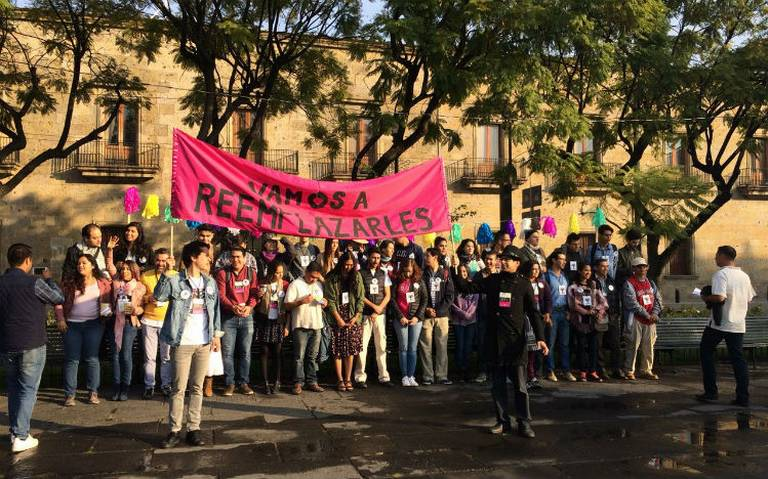
\includegraphics[width=\textwidth]{reemplazarles.jpg}
	\caption{¡Vamos a reemplazarles!}
	\label{fig:reemplazo}
\end{figure}

Para muchas de nosotras era inconcebible que un protopartido pirata se convirtiera en otro partido electorero aunque las personas que lo convirtieron en el fracaso electoral que fue, usaron diversas técnicas de la \hlfix{Ciencia Politica}{¿necesita las mayúsculas?} para conducir a toda la asamblea hacia su propio interés. El cambio de piratas a populistas se explica si pensamos que una organización es un juego con reglas formales e informales. En este caso, las personas más capaces decidieron renunciar a la consigna política que crearon, para usar el poder que les da pertenecer a una élite (familias poderosas, alta educación académica, carisma, estatura, capacidad para hablar, habilidades de negociación o de ciertas jergas populares y agendas consensadas en el movimiento \#YoSoy132) para perseguir su beneficio personal con una justificación mediática suficiente: \emph{somos las personas indignadas que se levantaron en México para denunciar todos los problemas y encontrar todas las soluciones.} Quizá muchas de estas personas ignoraban (y quizá todavía lo hacen) el aura de capital social que les rodea y que las hace prácticamente intocables frente al asedio de corporaciones económicas y partidistas, además de agencias de inteligencia que a lo largo de los últimos sesenta o setenta años se han dedicado a asediar e incluso asesinar a la oposición popular organizada (o sea a las organizaciones sin integrantes de abolengo) en México.

Para quienes nos posicionamos por la pregunta de cómo hacer efectiva y concreta esa otra forma de hacer política, lo primero que aprendimos fue
\begin{enumerate}
	\item que en México toda forma política es corporativa y está programada en nuestra psique a un nivel \hlfix{casi}{queda mejor decir \emph{prácticamente}.} inconsciente,
	\item a pensar en los problemas de responsabilidad individual como problemas que se pueden atacar cultivando nuestras potencias, fortaleciendo nuestras capacidades y reconociendo nuestras necesidades.
\end{enumerate}

No creemos en lo que mucha gente dice, que en México la gente es apática y apolítica. El espíritu agachado, arrabalero y huevón de que hablaba la filosofía ---priísta, por cierto--- del mexicano, y que todavía hoy constituye la ideología \emph{whitexican}, es en realidad la abnegación de sabernos sin las armas para combatir, de no querer que nuestras rebeliones no produzcan nada más que muertos y desaparecidos.

Sin embargo, a diferencia de hace unas décadas, hoy estamos en las condiciones tecnológicas para la conformación efectiva de un nuevo poder que cimbre el estado actual de las cosas. Para lograr una transformación real necesitamos accionar desde distintas aristas y facilitando la conexión estratégica entre distintos grupos políticos que buscan abrir y liberar flujos, que aumenten las potencias de las personas. La pregunta pedagógica es:

\begin{quote}
	¿cómo conciliamos todas estas cosas que hemos aprendido desde nuestra experiencia política con acciones articuladas y de gran escala, en diferentes niveles?
\end{quote}

Hay que darnos cuenta, por ejemplo, de que el rencor contra la partidocracia puede venir inconscientemente de desear el derroche, el exceso y el poder que esa gente tiene. En ese sentido, es importante hacernos \hlfix{la pregunta}{son más de una pregunta, sugiero ponerlo en plural}: si estuviéramos en sus zapatos, ¿cómo crearíamos otras formas de poder? ¿Por qué desearíamos renunciar a nuestros privilegios? ¿Cómo vamos a crear una cultura del encuentro y no del consumo?

La construcción de esta organización política es una metáfora del diseño de una nueva configuración del Estado que permita encontrar un más allá a la catástrofe, que reina a escala micro, \hlfix{molecular}{¿por qué molecular?}, local, y macro, \hlfix{molar}{¿por qué molar?}, \hlfix{global}{¿no será mejor usar el término en español mundial en vez de este falso cognado del inglés?}. Es necesario pensar cómo lidiar con los intereses de actoras individuales, cómo vamos a desarrollar todas nuestras capacidades orientadas hacia un cambio multidimensional, desde dónde lo haremos y cómo conseguiremos recursos.

Estas necesidades se pueden sintetizar, por ejemplo, como infraestructura tecnológica, para innovar con las herramientas que conocemos, gestionadas por \hlfix{geeks}{En cursivas, por ser anglicismo.} por ejemplo; cartografías del poder a través de visualizaciones, organigramas y diagramas de flujo desarrollados por economistas, abogadas y disenadoras; y documentación sobre los protocolos que dan vida a una organización resiliente, a través de procesos y patrones de trabajo.

Así, este texto pretende dar algunas luces a la cuestión de la crisis y la catástrofe, delinear algunos juegos de ficción utópica y posibilidades para empezar a configurar esos territorios imposibles. Desarrollamos algunos síntomas de la crisis política contemporánea, proponemos un modelo para tratar de navegar entre los múltiples factores que causan la opresión de las formas de vida, tanto en su relación con los gobiernos como con sus propios cuerpos. Esta posición escritural es \textbf{La Partida} y podríamos bien señalarla como especulaciones estratégicas, como una corriente de la táctica política. La pregunta central que guiará nuestras reflexiones es \emph{cómo nos organizamos} para un más allá de la catástrofe, cómo creamos un nuevo horizonte. Para nosotras, la estrategia consiste en acciones para visibilizar y combatir las asimetrías de oportunidades y capacidades de las personas y la táctica en configurar prácticas y patrones para las operaciones concretas en el territorio y fuera de él, partiendo del reconocimiento de las circunstancias de cualquier persona que actúa, de cómo en ella se entrecruzan múltiples fuerzas de captura a distintas velocidades.

\chapter{¡Estos son los problemas reales!}
\label{sec:probreals}

\section{El estado actual de las cosas}
\label{sec:stateart}

Aunque \hlfix{usted}{Siento que este recursos de formalidad rompe un poco con el tono usado hasta ahora.} no lo crea, no vivimos por sino a pesar del capitalismo. Se calcula que el ritmo de producción de la \hlfix{economia global}{economia mundial mejor, en español} necesita de aproximadamente \hlfix{cuatro planetas Tierra}{Recuerdo que el dato era de 7.5 para poder vivir de acuerdo al estándar norteamericano.} para ser sostenible.\addref{} La producción de imágenes para capturar el deseo de todas las personas y orientarlos a la acumulación de mercancías a través de la industria cultural nos hace desear el dinero para cumplir con un montón de estereotipos sociales impuestos por la publicidad. ¿Cómo? A través del miedo y la promesa de algún día estar por encima de las demás personas. Mientras, el trabajo se vuelve más precario conforme la optimización y automatización, administrativa y de procesos, se desarrolla en la \hlfix{economia global}{economia mundial mejor, en español}. A los desempleos masivos hay que sumar la incapacidad de los Estados de solventar las deudas sociales, de garantizar algún mínimo de estabilidad o de responder por la gente viviendo en la miseria. Nadie se da cuenta de que se enferma por el cambio climático porque no hay responsables aparentes para la contaminación y deterioro acelerado del planeta y de los recursos disponibles. El \emph{mainstream} tiende a asociar a la enfermedad con el azar o a la voluntad de Dios, una creencia azarosa que solo hace que las personas sigan aguantando las injusticias, para que sigan trabajando y comprando cosas que las hagan sentir valiosas.

A nuestros padres y a algunas personas historiadoras les encanta señalar que el mundo tiene un cauce definido. Sin embargo, saber cómo han sido las cosas en el pasado no significa que estemos condenadas a vivir lo mismo. Reconocer nuestro pasado es el mejor punto de partida para dar forma a un porvenir. Nuestra generación vive cada vez más la tecnología como una cuestión política. La potencia de la piratería y de los movimientos de código abierto (\emph{open source}) son ejemplos de cooperación más allá del mero lucro. Este es un punto de partida que nos da la fuerza para crear un movimiento que nos ayude a ocupar y abrir diferentes espacios. Las personas \emph{millennial} hemos nacido en una tensión histórica. Por un lado, tenemos acceso a un montón de información y un anhelo de libertad que nos impulsa a salir a la calle para encontrar una alternativa al presente. Por el otro, somos presas de la economía de la atención, personas adictas a interacciones virtuales y a códigos publicitarios cada vez más seductores.

\begin{figure}[htbp]
	\centering	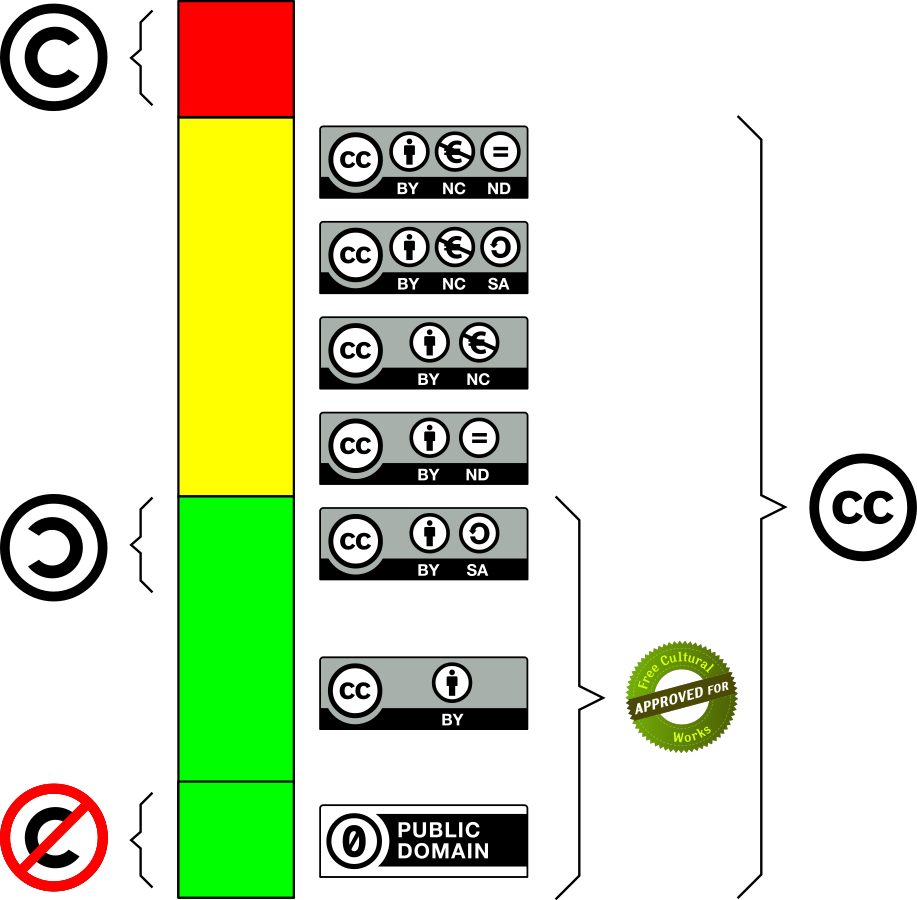
\includegraphics[width=0.8\linewidth]{creative-commons.png}
	\caption{Semáforo de licencias de Creative Commons.}
	\label{fig:CCsignal}
\end{figure}

Aunado a ello, las formas de violencia a las que son sometidas las personas son múltiples y complejas. Una apuesta política transformadora tiene que permitir reconocer estas violencias y dar herramientas para poder combatir. Queremos que todas podamos luchar.

Hay una diferencia abismal entre la violencia total, mutilante, hacia un enemigo abstracto (los criminales, las drogas, \enquote{el enemigo}\revquotes{}) y el roce propio del conflicto en la palabra, a través del habla y la escucha, mucho más vital y espontáneo, donde somos cuerpos que resuenan, que se transmiten. El problema es que nos enseñan que la violencia física, el poder del Estado, es la única manera de lidiar con nuestras diferencias, con nuestros deseos y con el desacuerdo. Para una transformación real, tenemos que \hlfix{hacer ingenieria inversa la caja negra}{O dices \emph{hacerle ingenieria inversa a la caja negra} o \emph{hacer ingenieria inversa a la caja negra}} y tratar de entender cómo se configuran las relaciones de poder y las reglas que dan sentido al Estado. Vivimos en una era en la que, con internet, robots y un sinfín de tecnologías, es técnicamente posible hacerlo. Se trata de permitir que todas las personas seamos co-creadoras de la realidad, que seamos potentes.

\section{Wikipolítica, ¿partido?}
\label{sec:wikipartido}

En 2018, Wikipolítica apostó todo por ocupar el Poder Legislativo en diversos estados de la República mexicana. Si bien no negamos que este es un paso necesario para proyectos de cabildeo estratégico, al no tener una visión de largo plazo, es decir, un programa de gobierno, nuestro experimento creó una red de voluntarias para salir calle a costa de reproducir las mismas dinámicas de explotación que cualquier trabajo o forma de activismo tradicional. Nos encontramos frente a un problema muy grave porque la energía de todas las personas decayó con nuestra terrible derrota en la contienda.

Frente a ello, la respuesta de algunas personas ha sido iniciar otro aparatoso e incierto proceso para crear un partido electoral. Desafortunadamente, el contexto del país es apremiante y la burocracia electoral es un camino de picar piedra. Vivimos una guerra que ha dejado cientos de miles de personas muertas y desaparecidas. Esto nos obliga a pensar en una alternativa radical al modelo extractivista, dependiente de los capitales financieros internacionales. Para muchas de nosotras esta guerra es invisible, pues, en efecto, es difícil reconocer que vivimos en una guerra por la fortuna de vivir en zonas seguras que están lejos de las huellas de la pobreza y la miseria, ya sea en otro país, en otra ciudad o simplemente en otro barrio. Nuestra incapacidad de verlo no significa que la crisis sistemática de derechos humanos, el exterminio feminicida, el auge del totalitarismo tradicionalista y el creciente poder de los capitales extranjeros no exista o vaya a terminar por sí solo.

La situación de nuestro país nos coloca frente a un problema de asimetrías de poder muy claro. Aunado a eso, desde 2016 este país se encuentra en un Estado de excepción. El despliegue y la militarización de las fuerzas del orden tienen como propósito hacerse del control territorial que el narco ha arrebatado al Estado mexicano, pero también para identificar, vigilar y repeler con hostilidad mortal a quien se oponga a los reptiles que pagan a las corporaciones armadas para velar por sus intereses.


\begin{figure}[htbp]
	\centering
	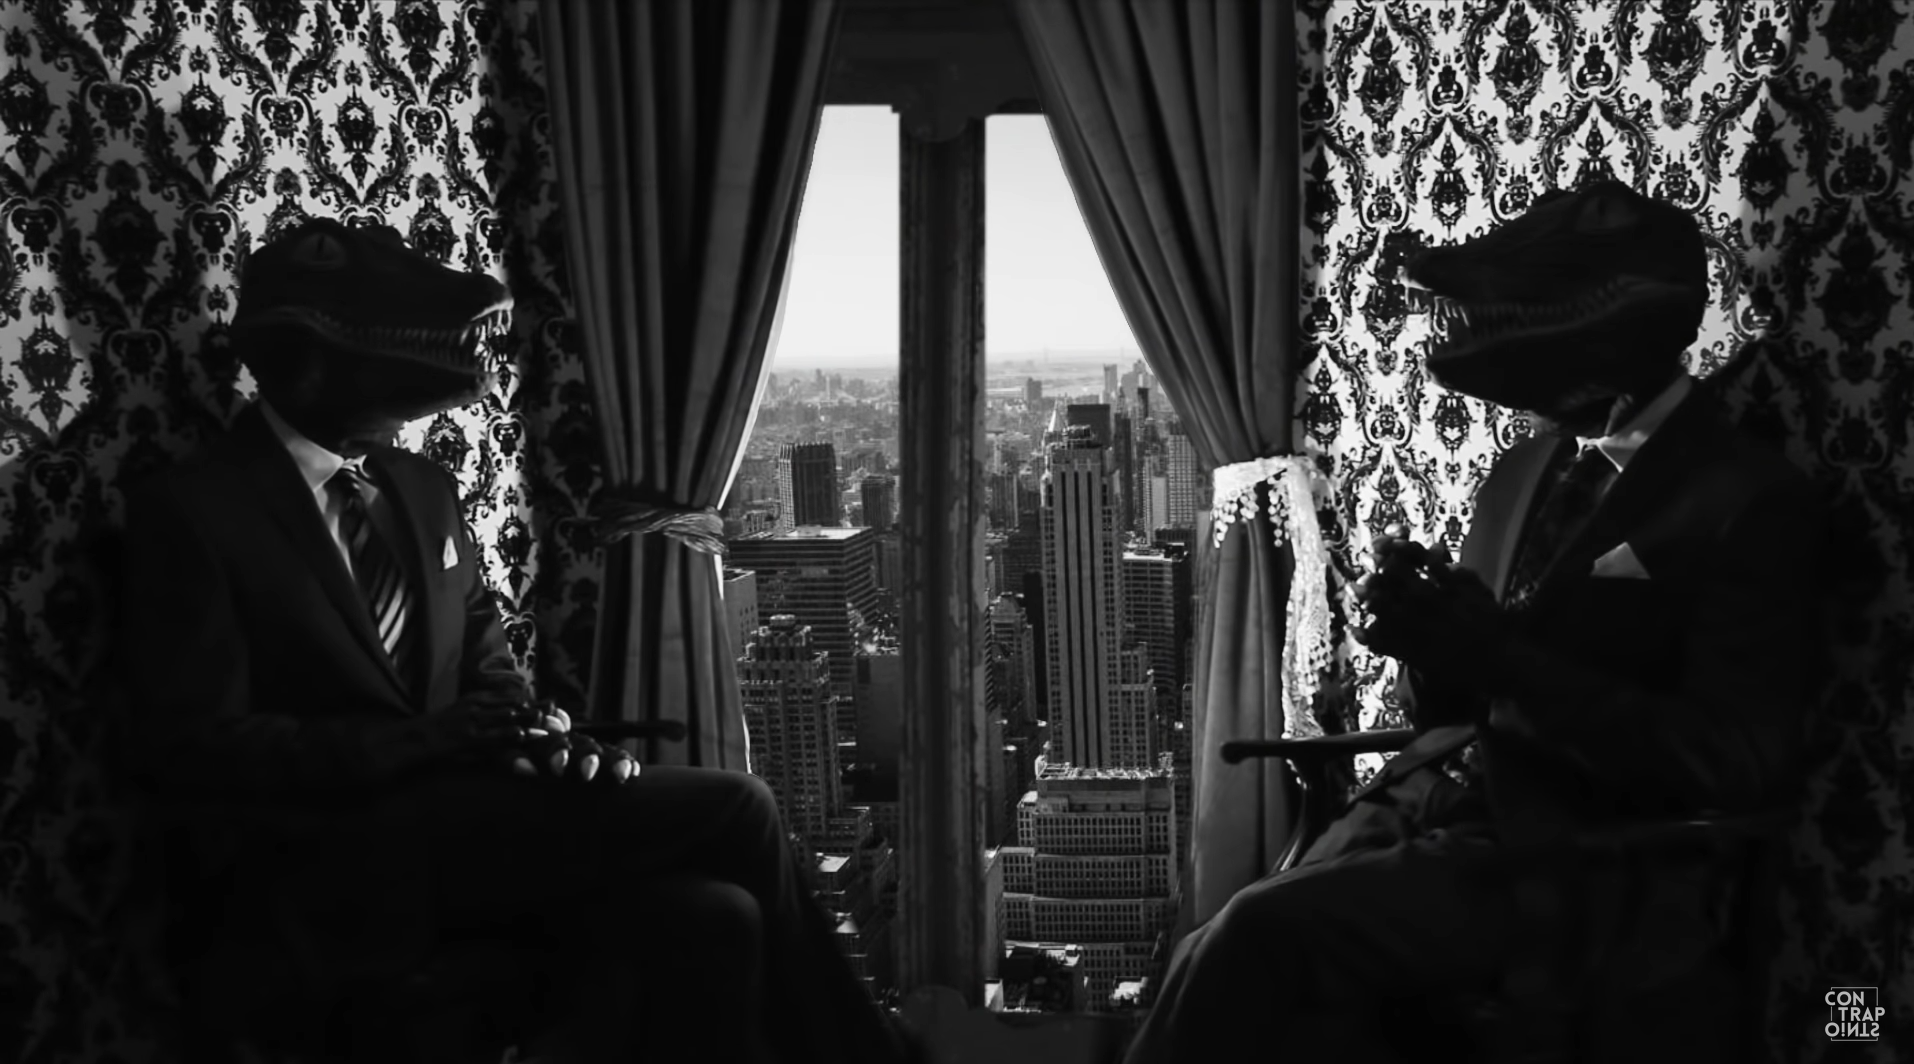
\includegraphics[width=.9\linewidth]{reptilianos.png}
	\caption[Reptilianos conspirando.]{Reptilianos conspirando. Mira \enquote{Lo malo del capitalismo} en ContraPoints de YouTube.}
	\label{fig:reptilianos}
\end{figure}

Ya, en serio, los reptilianos quizá no sean lagartos pero sí agentes de la utilidad, del plusvalor, es el 1~\% que siempre están buscando especular con su dinero para generar más dinero, a costa de quien sea y de cualquier daño al ambiente.

Volviendo al tema, la idea de un Partido meramente electoral es poco eficiente y bastante proclive al corporativismo patriarcal. Muchos machos adeptos a la disciplina del Partido hegemónico son también virilistas, amantes de la disciplina y el sometimiento al falo (al sacerdote, al patriarca), de la camaradería \emph{buenaondita} que invisibiliza las incapacidades de quienes asumen el papel de soldado \hlfix{razo}{Es \emph{raso} en realidad.} en un ejército de activistas. Como si de la disciplina y el control fuese posible producir otra cosa que no sea represión y esquizofrenia.

La historia no tiene un motor y cada cambio lleva consigo una posición sobre el presente, sobre el ahora. Lo único que nos permite creer en nuestra posición como \emph{La Partida} es la tecnocrítica, que significa que a cada instante nos cuestionamos cómo hacer cosas efectivas. Recuerden que la pregunta que nos hace pensar en el porvenir es cómo nos organizamos estratégicamente sobre los problemas estructurales que originan más formas de violencia. Si no pensamos así, seguimos en una cultura de la inmediatez que niega la magnitud y complejidad del problema, que sigue la corriente de los medios de señalar que no hay alternativas sistemáticas que nos muestren imágenes de otra sociedad.

Nos encanta la posición feminista que no encuentra sentido en la necedad electoral y en el deseo de Estado que late en la representación política. Nos parece que más allá de conquistar la hegemonía sobre \hlfix{UN}{hay que resaltarlo tal vez de otro modo} sentido común, se trata de crear canales por donde naveguen ríos de una multiplicidad de sentidos. Para nosotras, se trata de ir más allá de la vieja dicotomía izquierda y derecha. No queremos representar a nadie, ni gobernar, pero sí que nos preocupa la representación y el gobierno. Queremos que la gente recupere su propia voz, que ella misma pueda defender sus batallas, no queremos más paternalismos. Compartimos la lucha de la gente que pugna por una libertad radical, queremos dar voz, pero no partimos del dolor, partimos de la alegría y de la tecnocrítica como fe práctica, como creencia en la acción. Queremos que la gente pueda gobernarse maximizando la eficiencia de sus recursos y brindándoles nuevas herramientas. Sentimos que se trata de \hlfix{resetear}{Mejor decirlo en buen español: reiniciar} los símbolos culturales que existen alrededor de las herramientas que nos permiten gestionarnos. A lo largo de estos años, nos hemos dado cuenta de que es muy probable que las cosas que \hlfix{se te ocurran}{Contradicción con el tono usado al principio del capítulo que aparece en la primera nota del mismo.} para hacer un cambio suenen demasiado obvias, o sean muy difíciles o ya existan. En ese sentido, creemos que la tarea está en descubrir cómo hacerlas fáciles o que, si existen, sean conocidas por la gente que quieres que lo conozca, es decir, en crear una práctica de \emph{mainstreaming politics} (políticas sobre canales masivos).\footnote{Hemos pensado en estas prácticas como transversalización, basado en el criterio de la ONU sobre \emph{gender mainstream}.}\addref{}

\section{¿Qué tan efectivo es el activismo?}
\label{sec:activismo}

\begin{figure}[htbp]
	\centering
	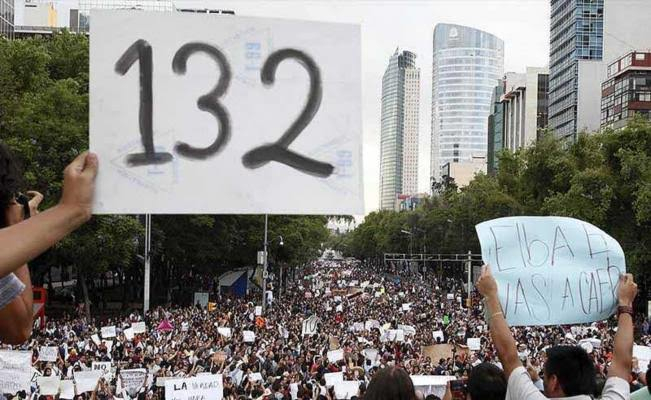
\includegraphics[width=.9\linewidth]{132.jpg}
	\caption{Asambleítis.}
	\todo[inline]{Mejorar la leyenda de la figura.}
	\label{fig:132}
\end{figure}

Los análisis de muchos activistas intelectuales de izquierda presuponen conspiraciones globales elaboradas, como si la estupidez global contemporánea fuera algo planeado. Ni siquiera los reptilianos en sus reuniones en Davos piensan en controlar al mundo. La modernidad es un discurso al cual aferrarse cuando en verdad el Medioevo nunca acabó. La aristocracia, la burguesía, la gente en el poder, son solo idiotas a quienes les gusta tener pisos de mármol, comer en restaurantes caros, vestir ropas caras y mirar sus números crecer.

\begin{quote}
	La verdadera tragedia del presente es lo que alguien llamaba la \emph{banalidad del mal}.\addref{}
\end{quote}

Mientras, nosotras vemos que el problema más grave que enfrentan las resistencias de calle es \emph{articularse} con otros esfuerzos. Muchas redes de movimientos de base, de activistas defensores de DD.HH., etc., tienen que trabajar con la sociedad civil, otra casta de aristoburguesía que actúa desde una clase privilegiada. Aunque no lo parezca, incluso en las resistencias pervive la lucha de clases.

A veces parece que entre las personas activas políticamente prevalece una atmósfera de rectitud moral, como si fuera evidente que lo que están haciendo para tratar de cambiar el estado de las cosas es lo correcto. En términos prácticos, resulta poco atinado querer imponernos frente a la gente, tomar nuestra visión política como algo evidente, con un vocabulario cerrado, cuando es una cosmovisión de clase (es decir, condicionada por nuestros hábitos de consumo y poder adquisitivo). La lucha es más eficiente entre más aprendemos a compartir, a socializar, a hacer un ejercicio mayéutico que le permita a la banda darse cuenta por ella misma de lo que quieres hacerle ver.

En este sentido, la militancia requiere aprender a escuchar a las personas para tener una aproximación más o menos clara de sus creencias para entender que la persuasión está en la apertura misma al diálogo. Después de todo, la libertad sólo existe en el momento en que somos capaces de tomar una decisión, y la lucha política es una decisión, nunca es evidente. Para empatizar, una tiene que posicionarse con \hlfix{ternura radical}{¿es esto un concepto acaso?} frente al otro. Hay que tener presente que las cosas que otras personas hacen tienen sentido de algún modo, al menos para ellas. En pocas palabras, no hay ninguna forma de vida que sea intrínsecamente más valiosa que otra. La clave está en reconocer los afectos como parte de la racionalidad política.

Mientras tanto, las personas afines al liberalismo (a la \hlfix{buenaonda}{en cursivas}, a la omisión del conflicto, a quienes reconocen que la única posibilidad es institucional) se retuercen frente a un momento de posverdad y de noticias falsas. No se explican qué llevó al mundo a semejante \enquote{irracionalidad},\revquotes{} no entienden que jamás la hubo y que los síntomas contemporáneos son también una oportunidad de crear un nuevo horizonte político. En medio de la crisis que vivimos diariamente, nuestra experiencia de la realidad como flujos de información (\emph{links, chats, shares}\ldots{}) nos da una capacidad que antes era imposible, para producir efectos en el mundo. Pero nuestra generación sufre porque somos conscientes del cinismo ilustrado que prevalece en el espíritu universitario, porque sabemos que tenemos el potencial técnico para vivir un mundo abierto, libre, pero no sabemos cómo (¿o realmente no queremos?) crearlo.

Nuestra visión de la estrategia simpatiza con una corriente conocida como xenofeminismo interseccional\addref{} y considera que las subjetividades están atravesadas por el género y por otras categorías que causan opresión en distintas dimensiones. La novedad radica en concebir estas categorías como dispositivos, es decir, como tecnologías que han sido diseñadas por alguien con fines en particular. El costo de nuestros fracasos al momento de actuar políticamente no es solo organizacional. Se trata, ni más ni menos que de una complicidad con el deterioro ecológico y la violencia interseccional (cuyo punto de culminación es la muerte) sobre las formas de vida, además del perfeccionamiento incesante y los procesos interactivos del parásito capitalista.

\begin{figure}[htbp]
	\centering
	
\includegraphics[width=0.9\linewidth]{xf.jpg}
	\caption{}
	\todo[inline]{Agregar una leyenda a la figura.}
	\label{fig:xf}
\end{figure}

\section{El cinismo es otra estrategia}
\label{sec:cinismo}

Hemos visto con tristeza que muchos movimientos políticos cargan con la melancolía de los vencidos, un estado de ánimo muy común a las izquierdas. Los hombres que lideran usualmente dan la apariencia del príncipe bucólico y carismático, como arquetipos del Che Guevara o de otros guerrilleros revolucionarios. A veces parece que el folclore que forman entre los grupos obedece más a su necesidad de sentirse abrazados por una comunidad de seguidores, a su incapacidad de superar sus traumas familiares o simplemente a cosas muy básicas como impulsos de destrucción o de tener sexo. Hemos visto muy pocas personas con un deseo genuino de crear una alternativa real, de actuar estratégicamente. Como lo vemos, los líderes machos se entregan al cinismo porque les es más cómodo usar la razón como instrumento para su beneficio. Estas personas se convierten en ideólogas, argumentan siempre en favor de lo que les conviene. Su postura es anacrónica, es decir, que no considera la evolución histórica ni las coyunturas que dan forma a las sociedades a través del tiempo, mucho menos considera que vivimos en una sociedad extremadamente compleja donde el capitalismo se manifiesta a través de algoritmos e instrucciones programadas en los comportamientos de las personas. Hay una estrecha relación entre esta posición de comodidad, de desvarío y de hipocresía irónica, y la crisis de fe contemporánea que hay que enfrentar para poder construir una alternativa. Por supuesto, el cínico reprimirá estos síntomas para seguir gozando de los beneficios materiales de hacerse pendejo, al costo de invisibilizar un montón de normas violentas necesarias para afirmar su identidad de macho ilustrado. Pero su posición significa varias cosas.

\begin{quote}
	Nota mental: \emph{El patriarcado no tiene género}.
\end{quote}

Por una parte, es la muestra de que vivimos un profundo vacío espiritual que necesitamos entender a través de sus síntomas para lograr crear una alternativa a la religión del Yo. Así como la teología de la liberación sirvió en su momento para la articulación política de subjetividades despojadas de su tierra, hoy necesitamos crear una nueva teología pop que haga frente a la falsa conciencia ilustrada contemporánea, que plantee un horizonte hacia la libertad a través de diferentes visiones religiosas, traduciendo ideas a través de significantes equivalentes.

\begin{figure}[htbp]
	\centering
	
\includegraphics[width=\linewidth]{century.jpg}
	\caption[\emph{The Century of the Self}]{El documental \emph{The Century of the Self} de Adam Curtis trata sobre cómo nació esa religión del yo.}
	\todo[inline]{Mejorar la resolución de la imagen.}
	\label{fig:century}
\end{figure}

Por otro lado, el peligro de estos hombres representantes es que su aliento heroico parece ignorar que vivimos en una guerra y que es absolutamente imprescindible tomar posición por acciones estratégicas que ataquen transversalmente varios problemas. Necesitamos entender que la evolución del capitalismo de \enquote{modo de producción}\revquotes{} a \enquote{modo de consumo}\revquotes{} y el paradigma de informatización de la economía, rompieron con la articulación de movimientos de clase, al estructurar la sociedad de tal modo que la identidad se configura a través de las mercancías consumidas y no de los vínculos afectivos entre personas. Accionar hoy requiere ser consciente de la lógica de la dominación contemporánea y no solo de las instancias tradicionales de incidencia.

\subsection{\emph{La verdad} es un instrumento}
\label{sub:verdadinstrumental}

\begin{quote}
	Hoy parece más fácil imaginar el fin del mundo que el fin del
	capitalismo.\\ \emph{Fredric Jameson}.
\end{quote}

El mundo no se acaba, se acaban las sociedades. Específicamente, se acaban quienes padecen las sociedades. Se acaba el hábitat de quienes solo tienen la tierra. La ecocatástrofe es la tragedia del exterminio de quienes viven en el margen, en las periferias. No es una lucha por la conservación del planeta sino por la vida de quienes padecen los residuos contaminantes del capitalismo. En medio de esta ecocatástrofe, la noción de \emph{verdad} tiene sentido para pensar en cómo se configura la memoria y la validez de los argumentos para un grupo de personas en particular. La verdad es el filtro con el que se mira, aquello que se considera valioso. Está relacionada con el recuerdo y está mediada a través del lenguaje, que articula nuestras experiencias en imágenes. La verdad siempre es a través de un observador, la verdad nunca está en el acto. En el acto hay presencia, realidad.

\begin{figure}[htbp]
	\centering
	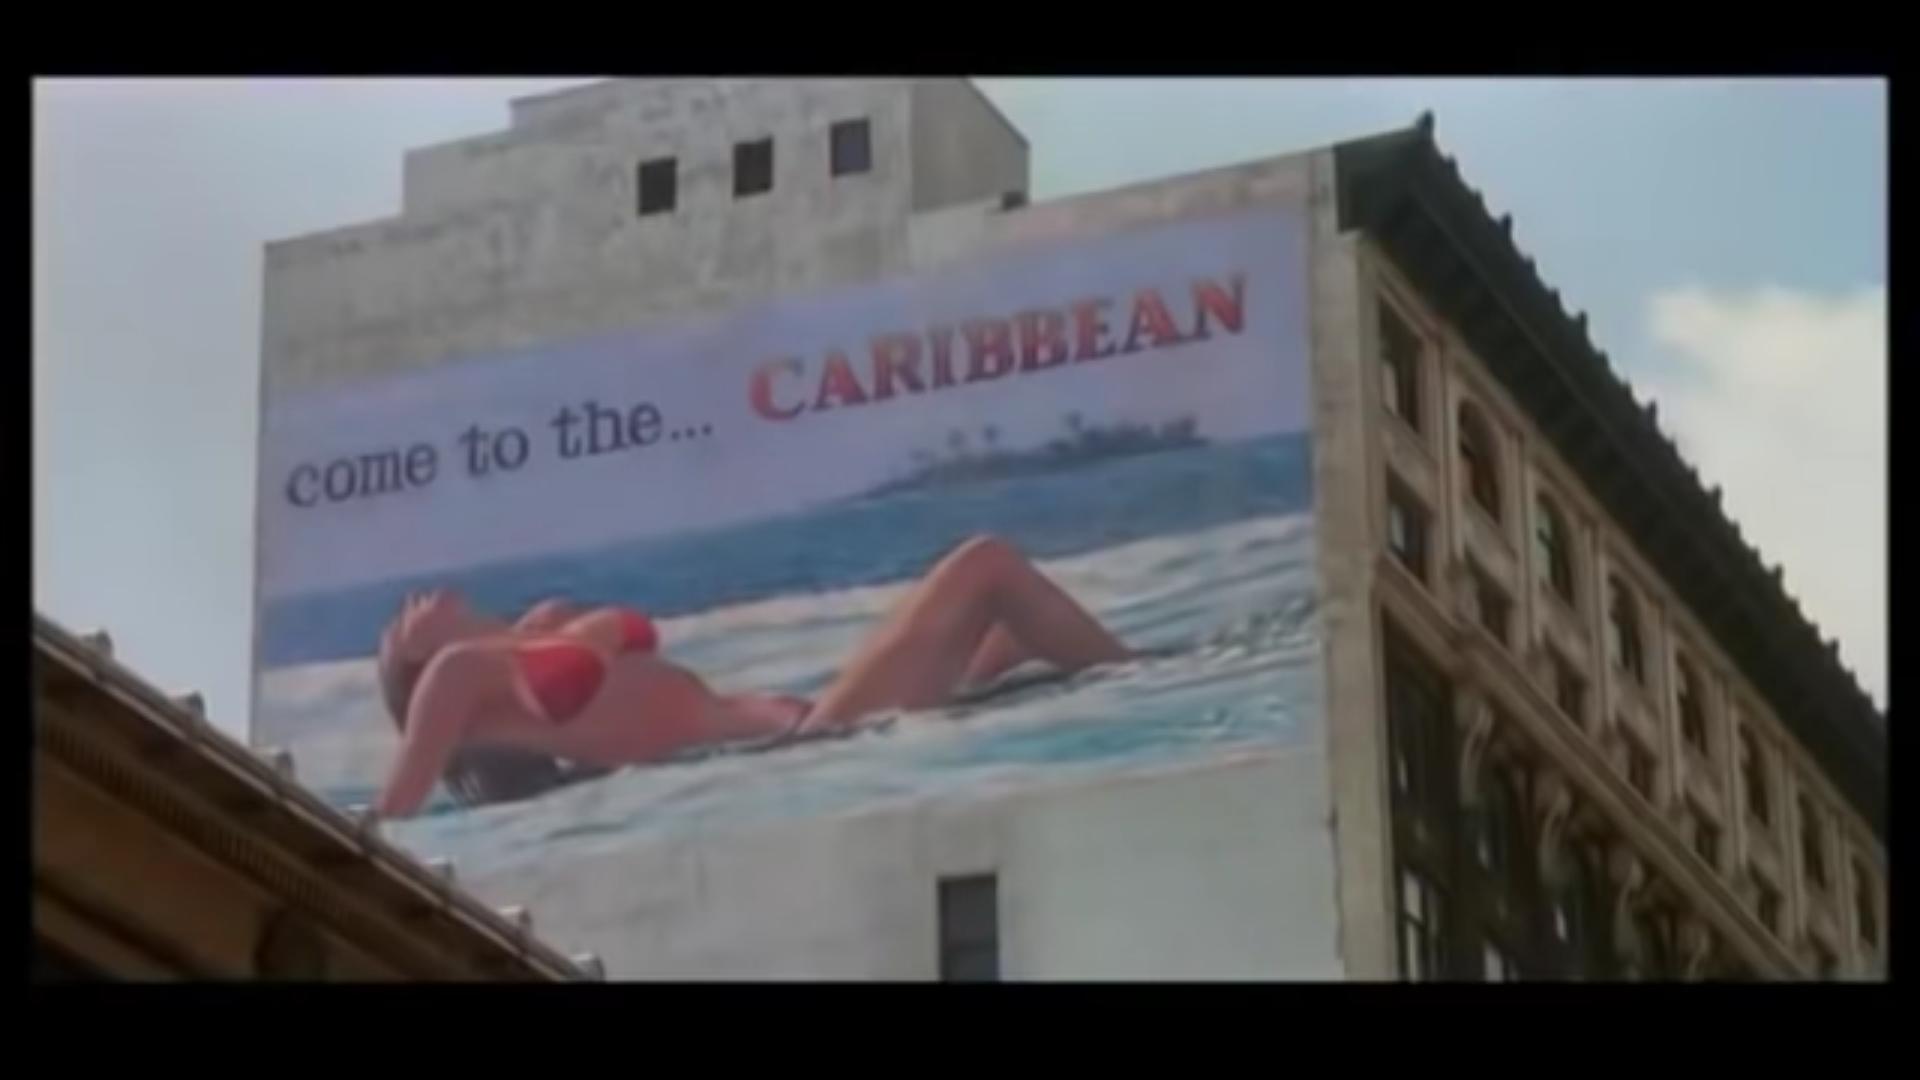
\includegraphics[width=.8\linewidth]{images/ideology1.png}
	\caption[Anuncio sin filtro.]{Anuncio sin filtro. De Slavoj Žižek en el documental \enquote{The Pervert's Guide to Ideology}}
\end{figure}

\begin{figure}[htbp]
	\centering
	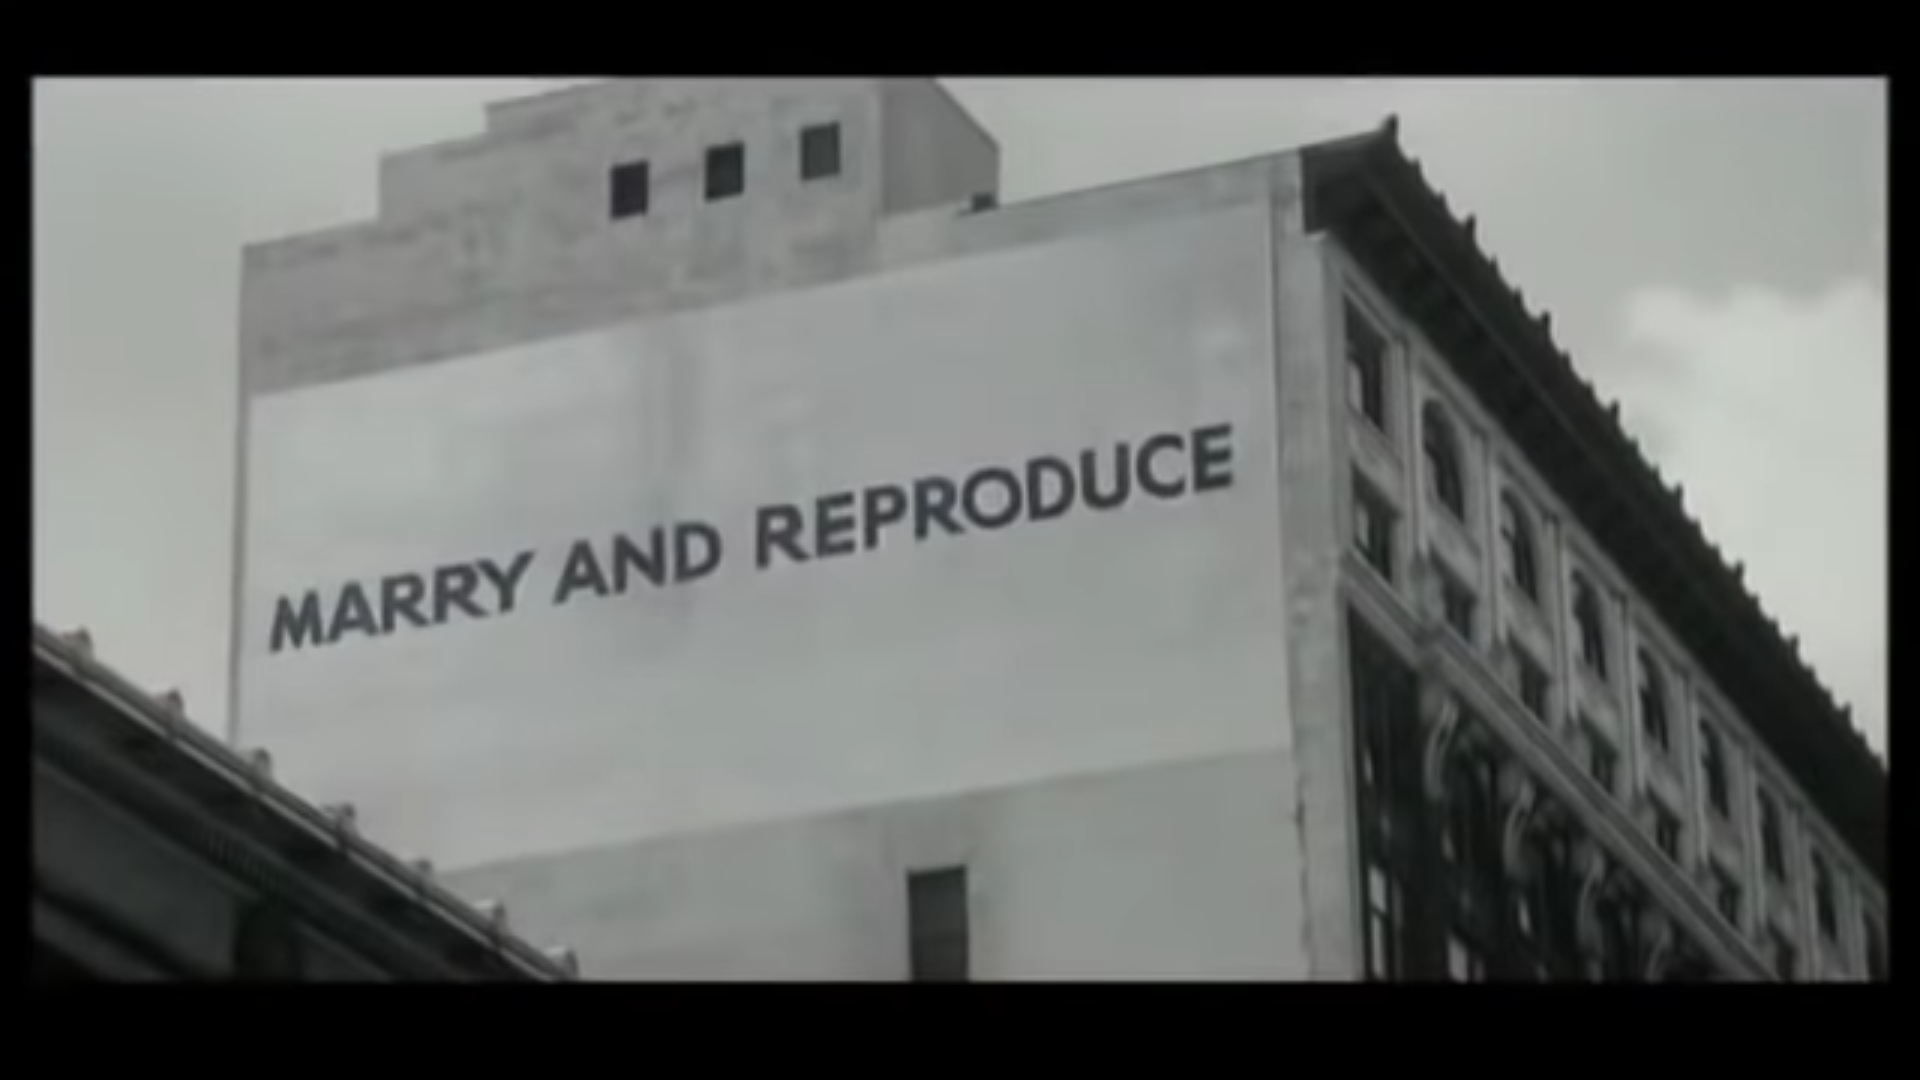
\includegraphics[width=.8\linewidth]{images/ideology2.png}
	\caption[Anuncio con filtro.]{Anuncio con filtro. De Slavoj Žižek en el documental \enquote{The Pervert's Guide to Ideology}}
\end{figure}

La noción de \enquote{conocimiento} proviene de una tradición de pensamiento que ignora otro tipo de \emph{saberes}, como la sensibilidad artística, la salud\footnote{Salud como buen vivir, por encima de la concepción que define la salud en sentido negativo, como ausencia de enfermedad, como lo mínimo necesario para que las personas estén aptas para producir. \url{https://www.theguardian.com/sustainable-business/blog/buen-vivir-philosophy-south-america-eduardo-gudynas}} o la relación con la tierra, la memoria y la conciencia sobre el territorio. Una militancia crítica, efectiva y consciente requiere la capacidad de comprender cómo se configuran los procesos históricos, testimonios y experiencias, de personas que hablan desde el lugar que habitan y cómo esa relación configura una identidad, no desde la historia oficial, de sucesiones de reyes y héroes grandiosos. Para lograrlo, es necesario renunciar a las pretensiones de verdad absoluta y a la culpa producida por la cultura del \emph{deber ser}. No hay una verdad por la cual luchar, hay verdades situadas según intereses. La tecnociencia es una herramienta transformadora, que puede servir para terminar con la escasez de alimento tanto como para perfeccionar un ejército. Es necesario asumir una posición en la que nada es evidente y todo acontece en la apariencia, obligándonos a estar atentas a nuestros juicios. El xenofeminismo nos permitió bosquejarlo como algo parecido a una pedagogía de la complejidad del mundo, que requiere una actitud casi estoica, contemplativa, de aceptación que hay que tener frente al mundo, como una postura de diálogo con la alteridad, con todo aquello que no es lo que creemos que somos nosotras individualmente.

La derecha alternativa (\emph{alt-right}) ha sabido bien utilizar la verdad como un arma. Dentro de este movimiento se critica mucho la idea de que la izquierda vive en una Catedral, haciendo alusión a una política dogmática y sectaria. Sabemos que esta postura no es otra cosa sino el partido del resentimiento total pero son, al mismo tiempo, tan básicos que nos han dado una buena idea, la de crear espacios como las Iglesias lo son para sus adeptos, pero para que las personas podamos hablar con libertad y recuperar vínculos entre nosotras. Si la derecha se vale de artimañas pos-ideológicas y adopta posturas económicas de la socialdemocracia keynesiana, nada nos impide reconocer que la justificación sobre el uso de determinada estrategia se construye después de que se ha obtenido una victoria. Por eso, si no pensamos en abrir las élites, en infiltrarnos, nuestro poder se verá reducido cada vez más. Las élites detentan el dominio material frente a los oprimidos a través de tecnologías como los códigos culturales del género, la raza o la clase. Sabemos que otras resistencias de izquierda más radical no han podido mantener un impacto, pero sí tecnologías de lucha avanzadas, como procesos, metodologías y códigos de programación que han resultado de distintas luchas de autogestión. No subestimemos sus esfuerzos. Estamos aquí porque hubo un Atenco, hubo una \emph{otra campaña}, hubo un Syriza. Esas luchas tienen que lidiar con el enemigo, quien en todo momento busca despojarle de su terreno, del patrimonio natural o de la vida misma. Ellas nos han enseñado que la autogestión no significa informalidad. Significa comprometernos a cultivar y entrelazar los saberes necesarios para que la gente pueda organizarse autónomamente con sus locales, con quienes comparte una vida común.

Sin embargo, la velocidad con la que la catástrofe ambiental y el cambio de lógicas de segregación a lógicas de gentrificación como forma de exterminio, devoran cada espacio donde es posible vivir, nos obliga a desarrollar tecnologías a gran escala que permitan conectar las resistencias locales a plataformas globales, con el propósito de atacar transversalmente estos problemas. Por ello creemos en una política de muchos frentes, multilateral, estoica y pragmática. Desde la izquierda y la derecha, desde arriba y desde abajo.

Hay que recordar, sin embargo, que muchas resistencias provienen de organización popular frente a los desplazamientos forzados por megaproyectos y otras imposiciones estatales. Frente a estas necesidades, es prioritario que pensemos el activismo político tratando de articular proyectos, siempre desde el territorio, creando vínculos comunes con gente que comparte agendas, o fungiendo como líderes comunitarias para resolver algún problema en común con los vecinos. Es decir, crear una base social de simpatizantes a través de la participación real en la comunidad. Una buena forma de hacer esto es, por ejemplo, analizando el código (los memes) que configuran una experiencia concreta de lo real para un grupo de personas y crear imágenes que la gente haga suyas sobre cómo organizarse, cómo participar desde su circunstancia particular, partiendo de comprender las motivaciones y necesidades de las personas. Saul Alinsky, un organizador comunitario muy importante en Estados Unidos durante la primera mitad del siglo XX, insiste en tener una ética basada en principios interpretables, no universales sino en tensión. A grandes rasgos, esto significa jugar un rol de mediador a través del reconocimiento de las diferencias y con entrenamiento para crear consensos y resolver disputas. Pero, sobre todo, reconocer que el \emph{trabajo} y la forma en que \emph{deseamos} son cuestiones clave para encontrar una alternativa a la crisis.

\section{Un trabajo político efectivo}
\label{sec:org0d34f13}

En términos concretos, necesitamos aprender a trabajar en calidad de iguales, a escucharnos y a delegar. La tarea es compleja y requiere acciones multidimensionales, desde distintos frentes. Por ejemplo, frente al panorama mundial, necesitamos dialogar con distintos movimientos alrededor del planeta, desarrollar una política internacional que podamos empujar y difundir en la opinión pública, abrir líneas de estudio y tender puentes con los diferentes sectores con los que estemos presentes. No necesitamos ser protagonistas de la lucha, como lo demandaría la ideología de la representación política, sólo crear las condiciones de posibilidad para que suceda. A esto nos referimos con la idea de abrir espacios para que todas podamos ocuparlos. Tenemos que ser estratégicas y usar con precisión herramientas de redes sociales pensando en hacer sexy el activismo/militancia política para más personas. Estas cuestiones nos abren preguntas de comunicación y mercadotecnia como:

\begin{itemize}
	\item ¿cómo nos diseminamos estratégicamente?
	\item ¿con quién queremos crear lazos?
	\item ¿cómo nos hacemos visibles para otras simpatizantes?
\end{itemize}

En función de nuestra capacidad de acercarnos a la gente que nos apoyaría, podemos encontrar alternativas de financiamiento, como la creación de un ecosistema de cooperativas donde las personas puedan ser consumidoras y productoras. Para lograrlo, podemos hacer labor política en nuestras redes para identificar prácticas y proyectos útiles, como los de sistematización de metodologías de organización o lo que ayude a que todo sea más democrático y eficiente.

La cuestión está en tratar de que todo lo común a nosotras (espacios, recursos, expresiones) tengan mecanismos efectivos de implementación local, que cualquier persona pueda acceder a nuestros recursos y organizarse. Esto es posible con una pedagogía de organización personal y comunitaria a partir de hábitos y prácticas. No se trata de compartir un canon ilustrado sino de descubrirse como manifestaciones concretas de la humanidad y trabajar entre todas para vivir alegres. Para ello tenemos que plantear del principio de que las organizaciones se planean y diseñan desde sus usuarias y desde sus operadoras. Esto significa que nuestros procesos también deben estar diseñados para \emph{nosotras, las personas} que los operamos. Con la intención de ser siempre una organización diseñada para la hospitalidad, para atraer la atención de todo el mundo y poder acercarle una vía para interactuar con la organización y participar políticamente desde su circunstancia.

\begin{figure}[htbp]
	\centering
	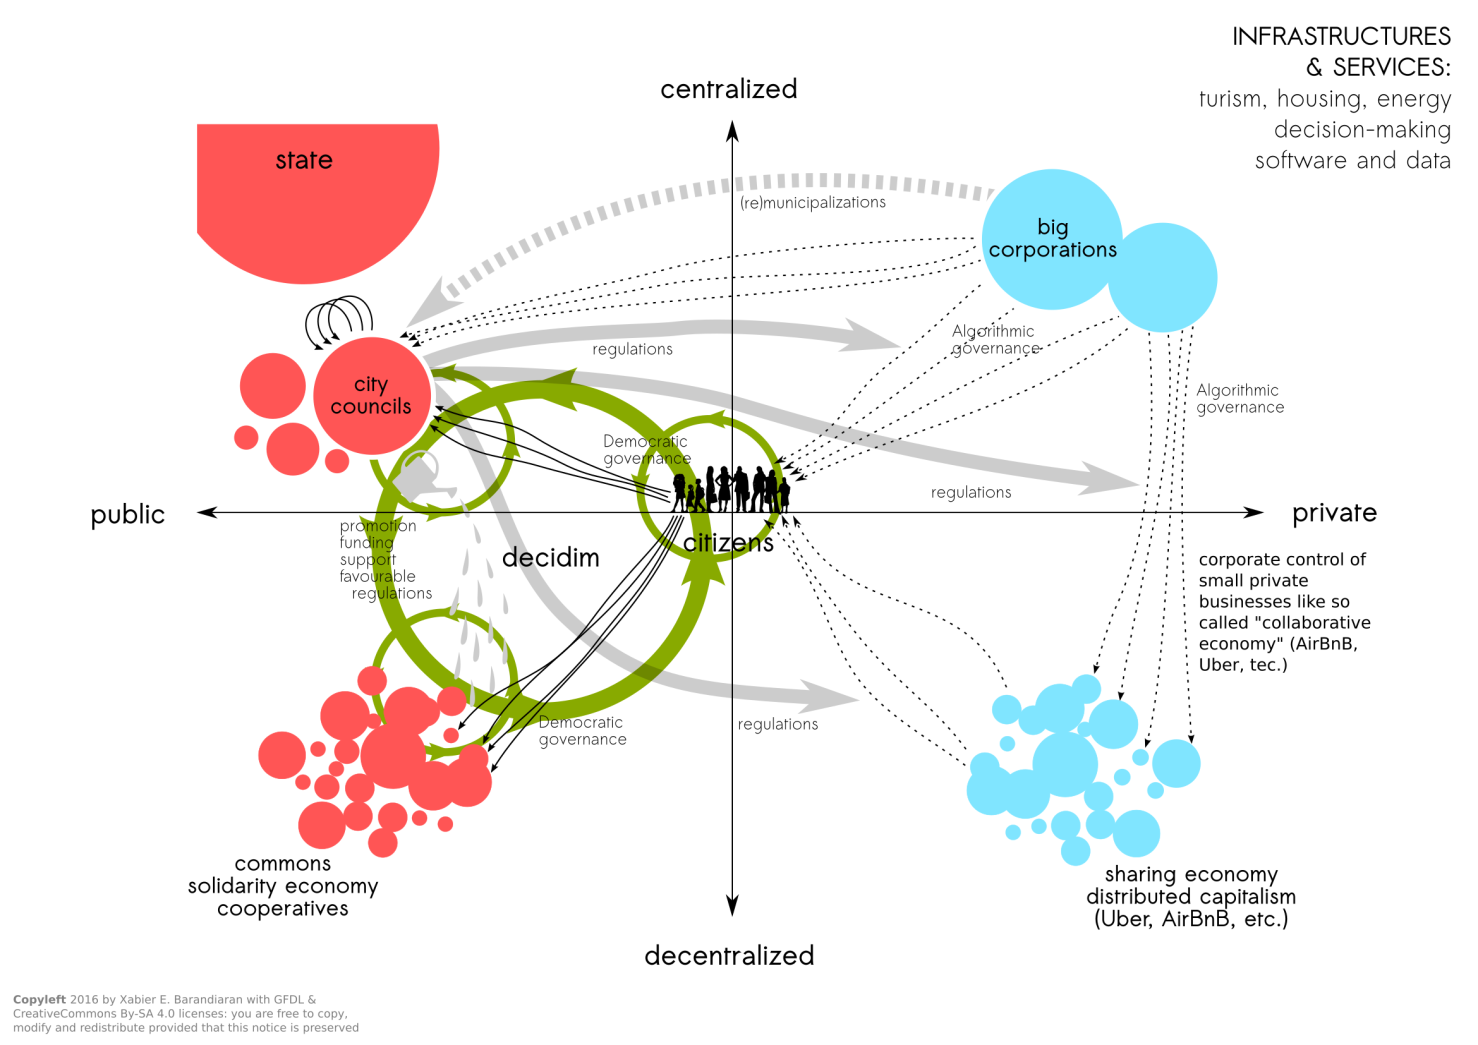
\includegraphics[width=.9\linewidth]{decidim-context.png}
	\caption[Proyecto Decidim.]{Un ejemplo de formas de organización social y el aporte del proyecto Decidim.}
	\label{fig:decidim}
\end{figure}

También necesitamos procedimientos de creación colectiva.\footnote{El proyecto \url{decidim.org} es un buen ejemplo de plataformas de organización colectiva.} Crear dinámicas, herramientas y saberes comunes, además de hacer un reconocimiento explícito de posturas ideológicas para que cada grupo pueda desarrollar su agenda y así crear un plan de trabajo global donde cada representación temática se encargue de desarrollar su agenda. En este sentido, vemos al liderazgo como encuentro y mediación que necesita que desarrollemos tecnologías de la presencia para diseñar espacios donde se pueda gestionar adecuadamente el conflicto. Se trata de construir desde nuestras diferencias y no a pesar de ellas, de reconocer que los qués se resuelven en los cómos, es decir, que los grandes conceptos abstractos se vuelven tangibles a partir de los detalles de implementación. Hay tribus donde los jefes de tribu son únicamente las personas que consultan y toda su autoridad se basa en opinar la manera más acertada de hacer algo sobre lo que deciden en concreto las personas que saben cómo hacerlo. Sería bueno que cada persona que integra una organización supiera un conjunto de habilidades mínimas, como liderazgo, comunicación, gestión del trabajo o programación, para poder crear equipos realmente transdiciplinarios ajenos a la necesidad de tener la razón, de tener \emph{la verdad}.

\section{¿Cómo crear una alternativa?}
\label{sec:alternativa}

El deseo de Estado es realmente el problema que más nos preocupa, por eso pensamos que la crisis de nuestro tiempo es una crisis de la imagen. A grandes rasgos, el deseo opera como una respuesta activa de nuestra psique a la impresión que las imágenes producen en nuestros cuerpos. El Estado reproduce el Patriarcado y funciona de maneras muy sutiles, desarrollando tecnologías que transforman nuestro deseo en un canal para la transmisión de mercancías, para que nuestras respuestas sexuales sean capitalizables como grandes masas de tráfico de información. Si la sensibilidad ha sido durante mucho tiempo una mera disposición pasiva al sufrimiento, ahora tiene que volverse el medio mismo del combate, ser una ciencia de la transmisión de imágenes y del hackeo de significados, ser la ciencia de los memes. El arte político de redirigir el sufrimiento en fuerza, el odio hacia uno mismo y los impulsos de autosabotaje en rabia hacia las normas impuestas por el mundo exterior, y la desesperanza en coraje para luchar por seguirnos encontrando y construyendo, aunque a veces sea difícil. Tenemos que aprender a reconocer nuestros deseos y a hackear el resentimiento de clase,\footnote{El resentimiento de clase es, por ejemplo, la envidia que te produce tener que usar transporte público todos los días y estar expuesta a asaltos mientras que la persona de al lado, o de la otra colonia, viaja con chofer privado en un automóvil particular.} así como darnos cuenta de nuestros privilegios y de la importancia de nuestra historia y de nuestra clase para la organización política.

La maquinaria estatal se encarga de orientar todas nuestras voluntades a proyectos que sirvan para construir un orden donde todas las personas son ciudadanas, sí, pero también son soldadas, consumidoras y espectadoras de lo que es producido como lo real. Necesitamos pensar el modo de generar un sentimiento de creación que no se sienta como el sentimiento de los débiles de la izquierda, que no se sienta como revolución permanente sino como un mundo nuevo que surge de las cenizas pero no tiene el martirio de la filosofía existencialista porque es un sentir comunitario, porque no tiene la característica del abandono que veían esos filósofos individualistas, un mundo que está vivo y presente, alegre.

Una verdadera alternativa es la creación de un nuevo poder, de comenzar a construir un mundo donde efectivamente quepan muchos mundos. Desde el contexto político latinoamericano, la construcción de un proyecto de país es parte de lo que llamamos \emph{poder constituyente}, una articulación política para un nuevo contrato social. Una coalición de fuerzas progresistas para una agenda de innovación estratégica cuyo fin sea hacer efectivo el buen vivir o bienestar para todas las personas. Esta multitud se articularía alrededor de agendas, sectores y esferas de acción basadas en recursos comunes y en la visión FLOS (\emph{free, libre and open sources}), un concepto que desarrollaremos más adelante. Esto significa desarrollar una base social a través de una plataforma que permita que la gente se organice, un imaginario común del futuro y un repositorio de tecnologías que permitan a la gente \emph{saber hacer}.

\setchapterpreamble[u]{%
	\dictum[Christiane Taubira refiriéndose al presidente Macron.]{Los fracasos políticos son temporales, pero las derrotas semánticas y
	culturales son dramáticas porque tardan más en revertirse.}
	}
\chapter{Lee esto antes de \emph{hacer} algo}
\label{cha:antesalgo}

El nuestro es un mundo de redes, navegable a través de teorías de la complejidad y del caos. Muchos procesos automáticos alimentan diariamente el flujo de operaciones de las infraestructuras (redes de abasto de combustibles, electricidad para servidores, satélites, líneas de internet) sin que haya realmente un responsable. Las funciones están programadas y los destinos predeterminados. Miles de variables interactuando entre ellas a partir de distintos nodos que envían información diversa y que demandan u ofertan certificados, \emph{requests}. La idea de la cibernética es dispersar para crear un caos gestionable, incluso automatizable.

\begin{figure}[htbp]
	\centering
	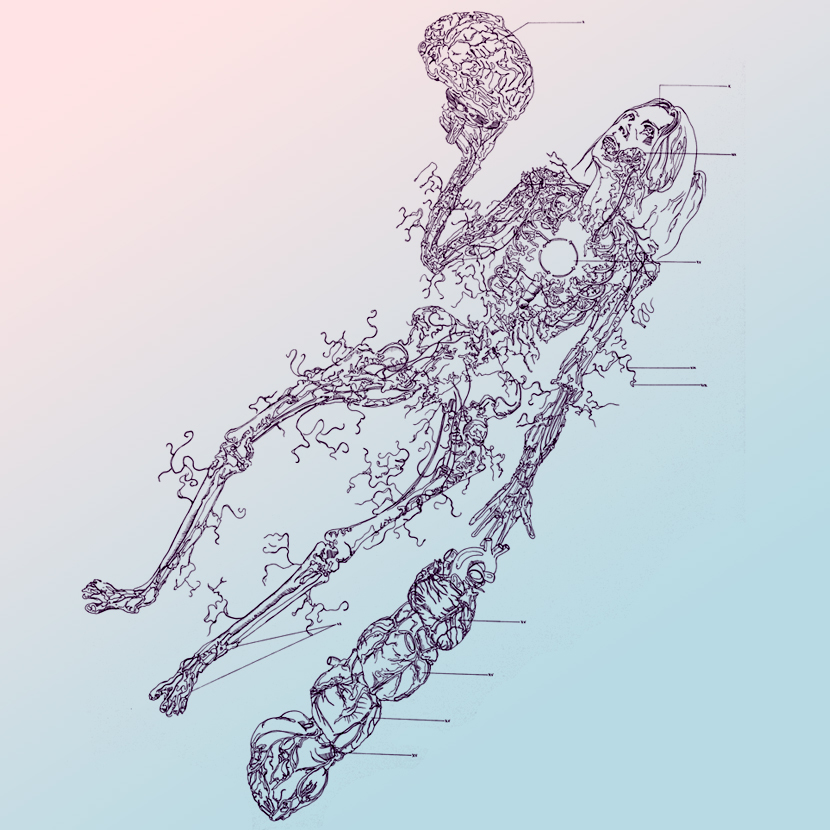
\includegraphics[width=\linewidth]{zombie.jpg}
	\caption{¿Cyborg o zombi?}
	\label{fig:cyberzombie}
\end{figure}

Al mismo tiempo, tenemos lo necesario para implementar una economía \emph{postescasez},\footnote{\url{es.wikipedia.org/wiki/Economía\_post-escasez}} sólo se trata de intervenir estratégicamente en esas redes de información, que también son flujos de sentido, producciones de deseo. La utopía robótica es una de las aristas de distintos escenarios posibles planteados por el texto de Peter Frese titulado \emph{Four Futures}, donde señala que viviremos en un mundo materialmente condicionado por dos aristas, una de igualitarismo-estamentalismo (o sea, donde las jerarquías manden) y otra de abundancia (por la automatización tecnológica) o escasez (por nuevas formas de los patrones para crear valor explotable). De esos casos, los más extremos parecen ser el mundo donde quepan todos los mundos, sostenido por una infraestructura tecnológica común, y el exterminio, que es prácticamente lo mismo, pero solo para el 1~\% de la población global.\footnote{A ello habría que sumar el problema del deseo, pensar en los desarrollos cibernéticos de las economías libidinales o economías del deseo.}

\begin{table}
	\caption{}
	\todo[inline]{Añadir una leyenda a la tabla. Se hizo flotante para poder asignarle una referencia cruzada y vincularla a la sección~\ref{sec:viruscapitalista}, donde se le cita.}
	\label{tab:Aristas}
	\centering

	\begin{tabular}{lll}
		\toprule
		 & \textbf{Abundancia} & \textbf{Escasez}\\
		\midrule
		\textbf{Igualdad} & Comunismo & Socialismo\\
		\textbf{Jerarquía} & Rentismo & Exterminismo\\
		\bottomrule
	\end{tabular}
\end{table}

Según Natalie Wynn\footnote{Famosa por ContraPoints, su vlog en YouTube.}, la derecha de internet pinta una caricatura de la izquierda, con el marxismo posmoderno como la supuesta ideología. Esto es muestra de que una de las operaciones más efectivas del parásito capitalista es poner a pelear a las resistencias en torno a cosas pequeñas y concretas,\footnote{Freud se refiere a esto como el narcisismo de las pequeñas diferencias.} cuando es más aquello en lo que estamos de acuerdo pero tenemos la necesidad de encontrar coherencia teórica en modelos ideales y no en especulaciones sobre la realidad. Esta posición que renuncia a la necesidad de certidumbre intelectual ---es decir, que no va más allá de una pregunta sobre instancias, sobre cómos--- se conoce como realismo especulativo y es cercana a una teoría del conocimiento (y filosofía del ser) llamada \enquote{ontología orientada a objetos}. Es importante recordar que probablemente las civilizaciones humanas han sido injustas desde el principio de los tiempos, pero la posición que tomamos respecto a la explotación de los patrones, de los propietarios o de los banqueros depende en buena medida de dónde estamos paradas.

Como reza el lema del xenofeminismo:

\begin{quote}
	\textsf{\textbf{Si la naturaleza es injusta, ¡cambiémosla!}}
\end{quote}

Podemos hablar desde el arte, generando consensos en torno a acciones comunes en distintos grupos. A veces parece más fácil actuar desde los medios que desde la militancia de izquierda. Nuestras aliadas han repetido ya varias veces la necesidad de hacer un posicionamiento estético sobre el discurso. En nuestros tiempos, en la política rige el principio de que fondo es forma. Y sin embargo, son las cuestiones estructurales como el género, el color de piel, la nacionalidad, el acceso a educación, salud, el dinero, etc, las que más afectan, por una cuestión de origen, de diseño, sobre las tecnologías que configuran nuestra realidad.

Al ser un concepto y no el nombre de un objeto concreto, la influencia del capitalismo se toma por la derecha como un mero principio económico que brinda todas las mercancías necesarias para vivir cómodo. He aquí una de las partes más importantes del problema. Para entenderlo, tenemos que comprender las diferencias entre Estado y Capitalismo en la historia, y cómo funciona a grandes rasgos el espectro político a partir de estas diferencias. Sin embargo, el pensamiento del \emph{status quo} es realmente poderoso pues el Estado dispone de manera muy particular de las armas que reproducen el modo de producción capitalista, las orienta siempre a la eficiencia y optimización que produce valor intercambiable.

\section{¿El enemigo es el capitalismo, el Estado o los mercados?}
\label{sec:enemigos}

Ahora vamos a profundizar en algunas distinciones que sirvan para hacer cosas que generen cambios reales. Sabemos que en este análisis hemos hablado poco del patriarcado, pues lo asumimos como parte de la ideología primigenia del capitalismo. Ponga usted mucha atención porque ahí vamos:

El capitalismo, desde una \emph{visión de ingeniero}, se trata básicamente de un modo de producción de bienes materiales. Este modo de hacer cosas parte de factores de producción que tradicionalmente han sido resumidos como tierra, capital y trabajo. El marxismo fue importante porque nos mostró un análisis mucho más extenso del capitalismo, al entenderlo como una configuración de las relaciones sociales a través de los procesos productivos, donde las mercancías tienen un valor por sí mismo y tan poderoso que configuran la identidad misma de las subjetividades.

Para nosotras, además de lo que le aprendimos al marxismo clásico, el capitalismo es un modo de producción, pero en este momento de la historia también es una \emph{velocidad sobre los flujos de información}. Para sostener lo anterior, es necesario que comprendamos que el viejo escenario económico donde la fábrica jugaba el rol predominante en la producción de valor ha sido reemplazado por una lógica de trabajo que pulveriza y divide en diferentes espacios la línea de producción, de manera que sea más eficiente y barato producir. Y lo que genera más valor en la economía contemporánea no es ya la mercancía como un objeto físico, sino la información que producen las relaciones entre las cosas. A esta era de la economía algunas personas la llaman \emph{posfordismo}, y entre otras cosas, es más una forma de producción regida por el consumo, es decir, la demanda de bienes, que por la producción, como lo fue en las revoluciones tecnológicas pasadas.

El mercado es un conjunto de transacciones. Es la infraestructura del intercambio mercantil y su acontecer capitalista tiene más que ver más con el cobro del impuesto, origen de la financiarización del valor,\footnote{Garzon Espinosa, Alberto. \enquote{¿Qué es la financiarización?} en \emph{Economía Crítica y Crítica de la Economía}. Disponible en:~\url{www.economiacritica.net/?p=144}.} que con el comercio. El capitalismo es un parásito cultural que paraliza el trabajo y subsume los recursos y hábitats del planeta mientras mercantiliza bienes primarios (\emph{raw materials}) en abstracciones virtuales, a través de una economía del deseo. Se in-corpora (es decir, configura una respuesta física, corporal) en las relaciones de las personas y crece sin límites hasta que mata al huésped. Además, es contagioso. Se ajusta a afectos y deseos de los huéspedes, mientras que se adapta a esa lógica en particular. Su funcionamiento produce un ecosistema. Imagina que además de una configuración sobre las velocidades, el capitalismo es un parásito que infecta los grupos sociales, una suerte de falla en la naturaleza que nos impide relacionarnos directamente.\footnote{Para ello, recordemos que la experiencia humana es tan antinatural, tan \emph{cyborg}, como una ciudad, como el internet o como la resina que implantan en tus dientes cuando tienes caries. Y que hablar de lo natural no implica de ninguna manera que algo sea justo. De ahí una frase que retoma el xenofeminismo: si la naturaleza es injusta, cambiémosla.} El propósito de este parásito es acumular cada vez más. La inteligencia del parásito reproduce la lógica de un virus informático. Es decir, hoy en día el capitalismo como parásito vivo es concretamente un algoritmo. Si la sociedad funciona como un sistema vivo, el capitalismo es el virus que infecta las relaciones sociales para convertirlas en relaciones mercantiles, con la única intención de mantenerse como necesario. En ese sentido, juega un rol parecido al Estado en la medida en que actúa como intermediario de toda relación social. Sin embargo, si el mercado es el medio del capital, \emph{el Estado es el soporte de información del mercado}, es el medio de almacenamiento y transmisión de la información del mercado que no puede ser retenida en la contabilidad. El Estado es una expresión de tecnologías del poder, con instancias materiales concretas. Más allá de la ideología, el poder se despliega a través de un conjunto de tecnologías.

El gobierno justifica la recaudación de impuestos al proveer servicios que hasta el momento consideramos que los mercados no podrán proveer (en buena medida por el control del capital). En términos de dinámicas de toma de decisión, el Estado es la masa personificada o \enquote{agenciada}, es decir, una entidad que puede trabajar como un agente. De ahí la necesidad de sistemas de recaudación en red que partan de una reconfiguración de las subjetividades y, por tanto, de la comprensión de lo público, lo privado y lo común.

\begin{figure}[htbp]
	\centering
	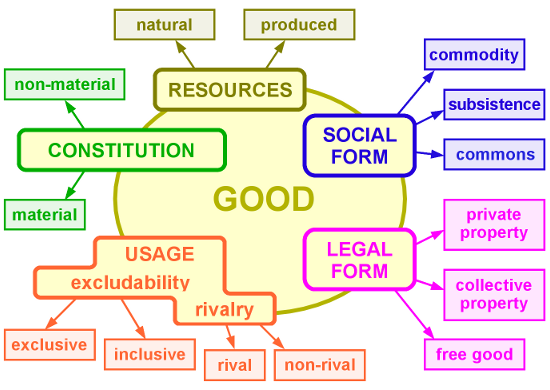
\includegraphics[width=.9\linewidth]{taxonomy-of-goods.png}
	\caption{Taxonomía de bienes o recursos.}
	\todo[inline]{¿Es necesario que el diagrama aparezca en inglés?}
	\label{fig:taxres}
\end{figure}

Volvamos a los factores de producción (tierra, capital y trabajo). El capitalismo necesita disponer de cada uno de ellos de forma que permitan producir más valor para generar más dinero y reproducir el ciclo de acumulación. Ahora bien, para que esto ocurra, necesitamos algo que muchas personas llaman contrato social, pero que nosotras preferimos llamar \enquote{reglas del juego}. Llamemos Estado a la entidad encargada de hacer valer las reglas del juego capitalista a través de las instituciones y de una maquinaria que garantice derechos de propiedad. El Estado proporciona lo que podríamos llamar \emph{aparato de captura} de los factores de producción para el ciclo económico del capitalismo.

Este aparato de captura se compone de tres subjetividades principales: el propietario (que posee la tierra), el banquero (que dispone del capital) y el patrón (que explota el excedente del trabajo). Estas personas (en su mayoría hombres, agentes directos de la estructura social patriarcal del ciudadano) son las cómplices humanas del parásito capitalista y se encargan de perpetuar su existencia garantizando la base material de la producción capitalista. Es decir, son los principales agentes vivos del capital y de su existencia depende estructuralmente la supervivencia del algoritmo. Hemos sido particularmente atentas en explicar estas cuestiones porque entre diferentes posiciones de izquierda (desde marxistas hasta anarquistas, pasando por feministas radicales y ecologistas) resulta extremadamente complicado distinguir al Estado del capitalismo o del mercado, y no podemos pensar en crear una fuerza política que produzca transformaciones radicales sin que entendamos de qué manera se implican estos sujetos en la configuración del estado actual de las cosas.

Hay una dimensión psicosexual de la producción, además de sus componentes materiales, a través del deseo. Todas las mercancías son un poco fetiches y actúan como mediadores sociales entre las personas. Las mercancías reflejan lo que las produjo: trabajo y deseo. La relación entre el parásito (capitalismo) y el Estado es simbiótica y no parasitaria. El Imperio es la forma que toma el Estado cuando el parásito muta de la fábrica al algoritmo. El parásito requiere al Estado para garantizar los derechos de propiedad de sus propios agentes.\footnote{(añadir de conspiradores y cómplices).} Estos sujetos son los traficantes de medios de producción y configuran el aparato de captura del Estado (lo que en una configuración urbana serían los muros o en una cárcel las cadenas). La forma algorítmica del parásito, a diferencia de siglos pasados, no reprime ni suprime más el deseo, sino que lo recodifica y se deposita en él. Sin embargo, la mutación del capitalismo produce fluctuaciones en el mercado, creando ciclos económicos donde el parásito es más fuerte pero también donde toca fonda antes de volver a mutar.

\begin{figure}[htbp]
	\centering
	\includegraphics[width=.9\linewidth]{algorithm-capitalism.png}
	\caption[El algoritmo virulento del capitalismo.]{El algoritmo virulento del capitalismo y sus conspiradores humanos.}
	\label{fig:algoritmo}
	\todo[inline]{Valdría la pena rehacer este esquema en español.}
\end{figure}

El parásito infecta a las personas a través de mercancías que producen interacciones sociales a través del intercambio. La persona asalariada, trabajadora, accede a intercambiar su fuerza de trabajo física, intelectual, sexual o la que sea, por la potencia abstracta del dinero y este por un objeto valorado socialmente que transforma la abstracción del dinero en reputación o prestigio, con el trasfondo del miedo a ser rechazada, a estar fuera del \emph{socius} si una no reproduce la transacción constantemente. De ese modo es que el capitalismo produce subjetividades a partir de la explotación de las trabajadoras, que en realidad no tienen una conexión real con lo que producen. En todo el planeta, aunque a diferentes escalas, esta forma de organización social produce al Gobierno y a sus súbditos: subjetividades caracterizadas por la fórmula \emph{ciudadano-soldado-consumidor-espectador}.

No hay posibilidad de una ciudadanía tal y como se concibe hoy en día al concepto dentro de los Estados liberales democráticos. La subjetividad del ciudadano (soldado, consumidor y espectador) presupone condiciones de clase, etnia y género muy particulares que básicamente se reduce al Señor blanco, heterosexual y cisgénero, que posee propiedades, es patrón de alguien y tiene acceso al crédito y a instrumentos más complejos en el sistema financiero. Además de que esta subjetividad plantea una relación con el cuerpo propio que niega su propia castración,\footnote{Toda mercancía, en la medida en que produce al sujeto como un objeto del valor de cambio de la mercancía, también produce entre sujetos una relación de objetificación. Esta forma alienada, instrumental, de comprender a la otra persona se reproduce en su comprensión de \enquote{lo real}. Es decir, que también produce una idea sobre la naturaleza. De ahí que el capitalismo no produzca otra cosa que hostilidad y desgaste, espacios inhóspitos, pues no concibe al mundo como otro sino como instrumento.} hace creer a la forma de vida que las otras personas son lienzos donde se dibujan sus fantasías frente a otras subjetividades pauperizadas que, entre todas, están construidas para satisfacer los deseos del Señor (¡sí, del Señor feudal, de tu papá y del señor patrón, y del señor de la casa y del Señor que reina en los Cielos, la palabra \emph{Señor} tiene toda esa semántica en tu cabeza!). Entender la realidad de ese modo, y en consecuencia, la Naturaleza (y a Dios, y a la Ciencia, y al progreso), solo reafirma el poder del Estado capitalista. Por ello, cualquier movimiento político que pugne por \emph{corregir al Estado} cuando este es la falla misma, terminará por infectar de deseos señoriales a las formas de vida que resisten a la subordinación del Espíritu que la sociedad moderna produce.\footnote{Aquí, la apuesta del populismo de Ernesto Laclau y Chantal Mouffe se posiciona por la resignificación de estos conceptos en el \enquote{sentido común}.} He ahí la complejidad de la práctica del cambio real.

\section{Más allá del Estado moderno: el Imperio}
\label{sec:imperio}

Desde un punto de vista estratégico, la transformación del Estado moderno, tras la consolidación del proyecto imperialista, es el Imperio. Esta forma se caracteriza por una pulverización del poder y un cambio en los modos de producción, donde se privilegian los procesos industriales pulverizados, sin fábricas ni obreros reunidos en un mismo espacio. El Imperio se caracteriza por el auge de entidades más allá de los Estados nación, como las empresas trasnacionales, que compran representantes políticos para legislar en favor de sus intereses. Aunado a lo anterior, la policía y la publicidad, mecanismos del Estado moderno, se transforman en el Biopoder y el Espectáculo.

El Biopoder consiste en el traslado del orden de La Ley a la regulación a través de normas sin sujeto, interiorizadas. Mientras, el Espectáculo consiste en la apropiación capitalista de la imagen para mercantilizar el deseo. Estos procesos maquínicos, que definen al Imperio como fase posterior al desarrollo e implosión de los Estados-nación, tiene distintos modos de regulación, que constituyen y dan forma a su aparato de captura:

\begin{description}
	\item[Aparato socio-ideológico:] familia, tradición, religión, nacionalidad, etc. Codifica el deseo y la colonización psicológica del sujeto, establece hegemonía, además de producir y mantener el estado actual de las cosas.

	\item[Aparato productivo-comercial:] finanzas, bancos, empresas corporativas, propietarios, etc. Comercialización de la producción, mercantilización del deseo para ligarlo al proceso de producción, monopolización del mercado, el valor de los desvíos que vuelve a los ricos a través de la parasitación de la mano de obra.

	\item[Aparato marcial-carcelario:] los militares, la policía, la inteligencia, el sistema de prisiones. Mantiene el estado actual de las cosas a la fuerza, la disciplina y el control de los sujetos, protege los intereses de los propietarios capitalistas y del Estado, sus fronteras, extrae recursos de otras regiones a través de la fuerza, redirige la riqueza para expandir el brazo militar del Estado e incentiva su investigación y desarrollo.

	\item[Aparato subversivo-periférico:] subjetividades colonizadas, grupos minoritarios, organizaciones criminales, la banda en sombra (\emph{shadow banking}), los mercados negros, etc. Muerte social y necropolítica. Establece la identidad de los ciudadanos mediante la otredad como diferenciación de subjetividades marginales, da un camino al lucro más allá del aparato comercial productivo.

	\item[Aparato legal de la soberanía:] el Estado, el sistema de justicia, los gobiernos, etc. Colonización, el espacio geofísico, establecimiento del territorio y determinación de estratos y jerarquías sociales.
\end{description}

\begin{figure}[htbp]
	\centering
	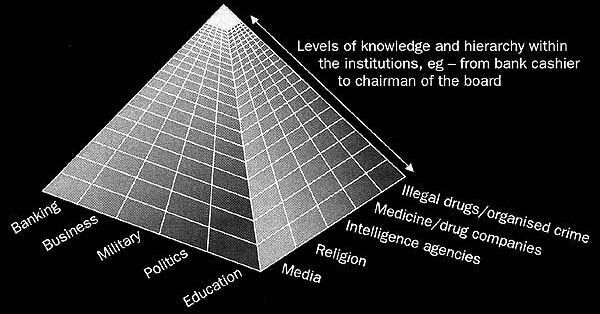
\includegraphics[width=.9\linewidth]{hierarchy-piramid.png}
	\caption{Taxonomía de bienes o recursos.}
	\label{fig:piramide}
\end{figure}

Si le damos una pensada más profunda y concreta, descubriremos que detrás de cada uno de estos dispositivos existen entidades económicas con transacciones y reglas del juego que regulan la vida social en diferentes esferas, pero a dos escalas, una micro (corporal, que corresponde al Biopoder y el Espectáculo) y macro (burocrática, de legislación e infraestructura tecnológica). En principio, podríamos hablar de las cinco grandes empresas que condicionan el desarrollo de las telecomunicaciones: Amazon, Apple, Google, Microsoft y Facebook. Estas son la base material por donde fluyen información y códigos sociales, representaciones del mundo, que son reproducidas en los dispositivos personales para provocar una reacción, un deseo. Esta nueva forma del capital explota reacciones, capitaliza el placer que puede cuantificar en \emph{clics} y \emph{shares}.

Este ciclo se basa en un delicado circuito de excitación, frustración y excitación que regula los hábitos de consumo. Se trata del modelo ideal de empresa neoliberal, un paradigma del negocio pos-industrial. La pornografía es un régimen estético que produce significados y un modo de presentación de las cosas que resulta adictivo, que permite obtener satisfacción del placer masturbatorio sobre la representación de cualquier fantasía posible materializada en videos.\footnote{De cierto modo, que el capitalismo se presente actualmente en su mayor apogeo a través de la industria farmacopornográfica (régimen toxicológico y semiótico-técnico), reproduce una concepción de la subjetividad como no castrable, cuyo horizonte parece ser el de autómatas dependientes del \emph{soma} de Huxley, personas discapacitadas, incapaces de habitar, de subsistir autónomamente.} En los foros de internet para varones adictos a la pornografía existe un nombre para el circuito pornográfico que tiene atados a tantos hombres a una forma particular de desear. Se conoce como: \emph{Porn, Masturbation, Orgasm (PMO)}.\footnote{Reddit. \emph{Don't lie to yourself\ldots P-M-O (PORN\ldots masturbation and orgasm) IS THE PROBLEM. Masturbation is just the symptom.} Disponible en \url{bit.ly/2HuEoem}.} El malestar de estos hombres cada vez más incapaces de vivir y en simbiosis con las comodidades del capitalismo que extienden el poder de sus formas tristes de vivir a otras esferas sociales, son el síntoma de este nuevo rostro de la economía. La excitación, la erección, la eyaculación, el placer y el sentimiento de autocomplacencia y control omnipotente se vuelven materias primas del proceso productivo.

\begin{figure}[htbp]
	\centering
	
\includegraphics[width=.9\linewidth]{nofap.png}
	\caption[Movimiento noFap.]{Movimiento noFap para hombres adictos a la pornografía y a la masturbación.}
	\label{fig:noFap}
\end{figure}

Por esta razón, P. Preciado señala que la pornografía es el rostro desenmascarado de la industria de la cultura y propone el concepto de \emph{farmacopornografía} para referirse al gobierno biomolecular y semiótico-técnico de la subjetividad sexual. Hay, de hecho, empresas que se encargan de regular la producción de contenidos excitantes que funcionan como mercancías con estudios explotadores y personas trabajadoras sexuales explotadas. La explotación mercantil del sexo es paradigmática porque un solo video puede producir millones de orgasmos,\footnote{Vale la pena revisar las estadísticas del tráfico de pornografía en internet. Por ejemplo, la información que libera \href{www.pornhub.com/insights/category/stats}{PornHub}.} lo que contrasta con la industria farmacéutica, donde el desarrollo de un medicamento cuesta muchísimo, pero es fácilmente reproducible una vez que se obtiene y patenta una fórmula.

\begin{figure}[htbp]
	\centering
	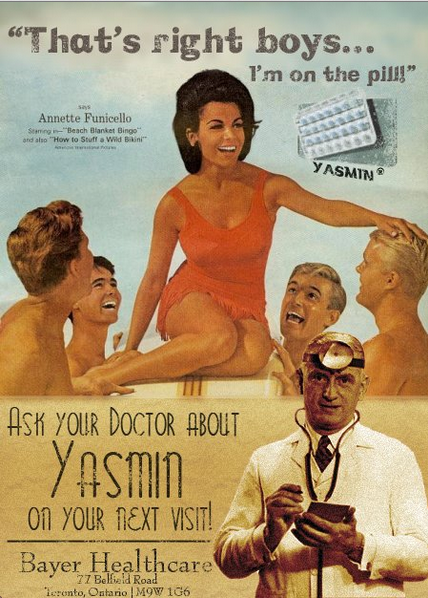
\includegraphics[width=\linewidth]{pillAd1.png}
	\caption{Anuncio de la píldora anticonceptiva.}
	\label{fig:anticonceptiva}
\end{figure}

\begin{figure}[htbp]
	\centering
	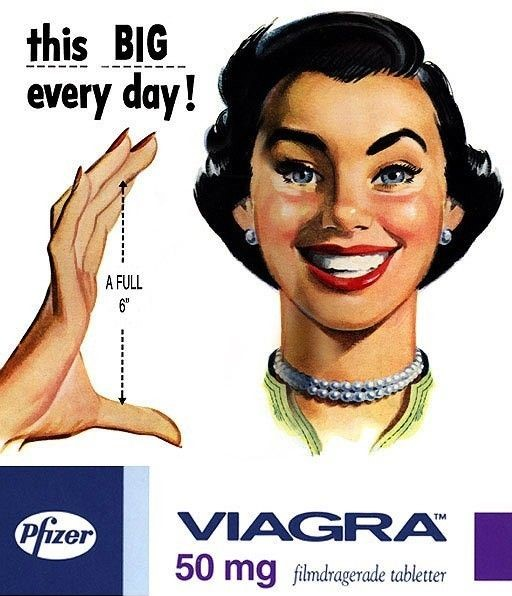
\includegraphics[width=\linewidth]{pillAd2.jpg}
	\caption{Anuncio del viagra.}
	\label{fig:viagra}
\end{figure}

Así, las grandes entidades económicas capitalizan problemas clásicos de la economía como las asimetrías de información, el problema de agencia o los dilemas de acción colectiva. Además, condicionan nuestros deseos imprimiendo en nuestras psiques imágenes de lo deseable, además de crear una erística que nos enseña que esos estímulos que aprendemos a desear los podemos obtener a través de la moneda, de intercambios mercantiles. Estas empresas aprenden, a través de costosas investigaciones sobre el comportamiento humano, para reproducir la servidumbre en los contenidos a través de segmentos de mercado donde se puede insertar el discurso del parásito capitalista bajo distintas situaciones y formas sexuales. PornHub es el paradigma de la industria cultural por su capacidad para producir orgasmos, para \emph{gestionar el género, la excitación, la frustración y el placer}. De este modelo de empresa se pueden extender otras versiones \emph{soft} (o blandas) que operan en otros aparatos sociales. Disney como el dispositivo que reproduce el imaginario de la jerarquía social a través de sus mitos de princesas, reyes y monstruos; MacDonalds y Coca Cola para reproducir la \emph{Resaltar en cursivas.}.\footnote{Es decir, la enfermedad de la impotencia, del cuerpo enfermo, pauperizado, envenenado por las bombas mediáticas que producen la comida rápida o chatarra como lo deseable, como el lugar a donde gastar el salario. Se trata de un régimen alimenticio de productos vacíos, compuestos de harinas, grasas, azúcares y otras sustancias que funcionan bajo el mismo principio de estimulación-malestar y que producen serios daños al cuerpo a largo plazo. El paradigma mercantil de la comida en tiempos del Imperio.}

\begin{figure}[htbp]
	\centering
	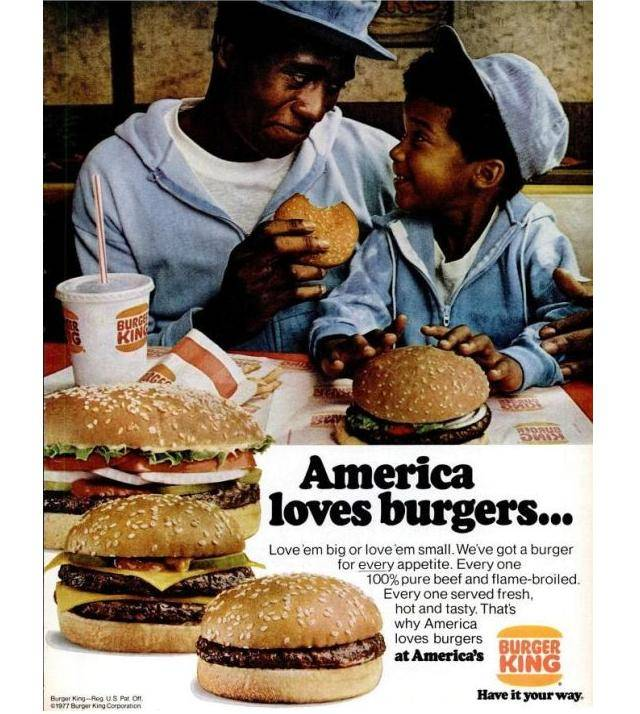
\includegraphics[width=\linewidth]{burguers.jpg}
	\caption{¡América ama las hamburguesas!.}
	\label{fig:burger}
\end{figure}

\section{La vida como trabajo y la producción de subjetividad}
\label{sec:subjetividad}

Un punto importante para comprender la transformación del Estado-nación al Imperio se encuentra en el papel del trabajo. Por ello, en este apartado analizaremos las condiciones de producción del trabajo del hombre-masa en la era cibernética. Para comenzar, tenemos que recordar que la dominación mercantil tiende a expandir sus dominios a toda área de la vida y al hacerlo vuelve trabajo a cualquier acción sujeta de la explotación. Este proceso está relacionado con la transformación de la subjetividad. No por nada el concepto central de las revoluciones de los siglos XIX y XX es la masa, una subjetividad que experimenta la realidad de la misma manera, a través del \emph{consumo estandarizado}. En este proceso, las vivencias en su forma de experiencias cognitivas dan sentido y estructura a la imaginación, es decir, a la máquina deseante que es cada singularidad. Así se configura una idea del pasado (a través de Hollywood que nos enseña a desear melancólica o espectacularmente) y del futuro (el apocalipsis como una finalidad de la historia implícita en las narrativas culturales a través del tecnocapitalismo, donde la explotación se extiende a cada rincón del planeta, deja a su paso desolación y muerte para después reconstruir la \enquote{sociedad}) a través de los medios que producen para las grandes audiencias.\footnote{Que dan forma a la cultura popular y al espectador televisivo en un circuito que lo posiciona como ente pasivo sentado en un sillón consumiendo comida chatarra.}

En términos concretos, la masa es el resultado de un proceso sintético en el que el individuo afronta una situación externa a él, participa en la situación y proyecta la situación en otros individuos que habitan el mismo espacio. Como ejemplo está Disney, que transmite efectivamente el deseo de casta a través de sus figuras de princesas, reyes y caballeros. Para profundizar sobre estos puntos conviene revisar los documentales de Adam Curtis, particularmente recomendamos \emph{The Century of the Self} y \emph{Hypernormalisation}.

\begin{figure}[htbp]
	\centering
	
\includegraphics[width=.9\linewidth]{complicated.jpg}
	\caption[\emph{Hypernormalisation}]{Toma de \emph{Hypernormalisation}.}
	\label{fig:hypernormalisation}
\end{figure}

Nosotras hemos intentado perfilar a la subjetividad ideal del Estado moderno como algo parecido al \emph{ciudadano-soldado-consumidor-espectador.} Solo basta recordar que el antecedente histórico del ciudadano han sido los súbditos, los fieles. Quizá desde ahí se perfila el proceso donde las multitudes devienen siempre masa a través de los aparatos de captura. El lenguaje cotidiano es muy útil para hacernos ver cómo se transmite la deuda en la subjetividad de ciudadano-soldado-consumidor-espectador:

\begin{quote}
	paga tus impuestos\\
	sirve a la patria\\
	no te pierdas el descuento\ldots{}\\
	ni el siguiente show (la siguiente película).
\end{quote}

En esta fórmula todas las personas deben. El deber y la deuda provienen del mismo sentir (y de la misma locución latina \emph{debere}). Sin embargo, la deuda tiene una condición que ha sido entregada antes del nacimiento, como una suerte de fruto por el que hay que pagar con el pecado original durante el resto de nuestras vidas. El ciudadano \emph{debe} pagar sus impuestos, el soldado \emph{debe} honrar a la Patria, el consumidor \emph{debe} comprar y el espectador \emph{debe} mirar.

\section{Hoy en día, el capitalismo se comporta como un virus}
\label{sec:viruscapitalista}

El algoritmo del virus capitalista y el condicionamiento de desarrollo de las tecnologías mediáticas para el excedente configuran lo que se espera de las personas individualmente a gran escala. Si bien los Estados-nación dieron forma a las revoluciones burguesas, fue en parte por la capacidad de leer la prensa escrita como criterio de consumo literario común suficiente para dar forma a una identidad colectiva, a una identidad de clase. Después, la radio y el cine también configuraron el potencial revolucionario de las comunicaciones. Por ejemplo, el radio creó un espacio informacional nuevo (urbanismo y psicogeografía). Esto nos muestra cómo una forma mediática representa poder y nos revela el papel clave de los \emph{medios}. Lo hace configurando el espacio a través de flujos de comunicación. La configuración de estas redes de comunicación es un catalizador para el cambio social (tabla~\ref{tab:Aristas} página~\pageref{tab:Aristas}).

En la actualidad, los modelos de masa donde un grupo recibe una sola transmisión son reemplazados por modelos donde el individuo recibe una transmisión única gracias a algoritmos reactivos que alteran la secuencia del contenido de las redes sociales y de ese modo individualiza y hace única la experiencia de consumo de cultura. La subjetividad ya no es producida como individuos en serie, sino a través de segmentos.

El cambio de paradigma de modelos de gobernanza en masa a modelos en red obedece al desarrollo cibernético del algoritmo. Las sociedades disciplinarias y de control son demasiado complejas para gestionar, por lo que es más fácil fijar protocolos para gestionar redes de manera más eficiente. El espacio masivo está condicionado al número de participantes en un espacio y un momento particulares, mientras que el espacio de redes se extiende y contrae en el espacio-tiempo de acuerdo a las órdenes y necesidades de la red. Es decir, su uso del capital es más eficiente porque se ajusta a las necesidades de cada momento.

Hasta ahora, este capítulo ha sido fuertemente influenciado por textos apócrifos de \#altwoke. Una idea discutida por la wikiPartida (una instancia de la Partida compuesta por gente de Wikipolítica) a partir de lo expuesto es que los modelos de gobernanza en red pueden desarrollar y expandir una cultura a través de \emph{labels}, donde los participantes son suscriptores de esta. Esto para hacer frente al problema de cómo se desplegaría una identidad FLOS que transmita cierta disposición práctica en los logos de organizaciones que la adopten. Por otro lado, nos surgen preguntas referentes a la cuestión de los medios como:

\begin{itemize}
	\item ¿qué ocurre con los gobiernos coloniales con el consumo de medios si hay masas y segmentos conviviendo y entrecruzándose? Nos referimos a medios como Netflix, Spotify y plataformas en línea, además de Disney, DirecTv, Warner o, en el caso de México, Televisa.
	\item ¿Cómo se configura el imaginario de las personas en México entre Facebook, Twitter, Instagram o YouTube, por un lado, y Televisa, como el monopolio de sentido durante el siglo XX, por el otro? Sin mencionar a Bimbo, Walmart, Coca Cola y otros grandes leviatanes.
\end{itemize}

\section{Alternativas económicas para el futuro}
\label{sec:altfutur}

\begin{figure}[htbp]
	\centering
	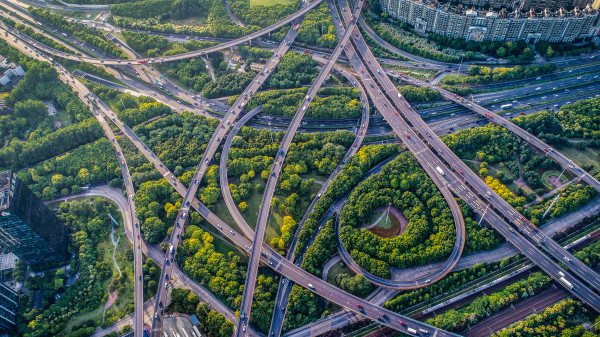
\includegraphics[width=.9\linewidth]{roads.jpg}
	\caption[\emph{Hypernormalisation}]{Toma de \emph{Hypernormalisation}.}
	\label{fig:hypernormalisation2}
\end{figure}

Hemos visto que en el entramado de complejas tecnologías que dan forma al presente, resulta extremadamente difícil accionar sin reproducir la lógica de la sociedad mercantil. El Estado, los mercados y el capital producen en conjunto una sociedad unida por un acuerdo económico donde la ética tiene un papel tan nulo que debe ser enunciada a través de imperativos morales universales porque nadie cree en ella. Y esto porque la sociedad es, en realidad, un arreglo para dar vida a las mercancías. No hay nada vivo ahí. Tiqqun acertó en señalar que la antítesis del comunismo no es el capitalismo, sino la economía, y que lo que es necesario derrumbar es la dominación mercantil, que se asume como realidad última de todas las formas de vida y de todas las cosas. Para concebir acciones efectivas y críticas, tenemos que considerar que nuestras prácticas deben rebasar las estructuras formales e informales que reproducen al parásito capitalista. Para ello es de gran utilidad asumir una visión interseccional centrada en la \emph{interacción entre violencias estructurales (género, raza\footnote{Hemos utilizado la palabra raza para referirnos al discurso de raza, una ideología biologicista que sirve a los patriarcas blancos para justificar la opresión a grupos étnicos o a cualquier forma de vida no-blanca.} y clase), dispositivos sociales, el aparato de captura del Estado, la cadena de producción del capitalismo contemporáneo y el algoritmo del virus capitalista}. Esto en un contexto de complejidad donde la producción económica es comprendida en buena medida como informática, como flujos de datos con potencial de explotación. La visión de la economía neoclásica, que al informatizar la economía, le da forma de cibernética, también puede ser una herramienta de sabotaje si pensamos en los problemas de acción colectiva que necesitamos resolver para combatir la dominación mercantil como problemas de información. Algunos ejemplos que pueden ser analizados bajo esta óptica son:

\begin{description}
	\item[Gobierno representativo:] entender a los representantes como traficantes de información sobre los incentivos de sus representados (lo que en economía se conoce como \enquote{problema de agencia} o \enquote{problema de agente-principal}).

	\item[Burocracia:] cualquier burócrata sabe que una parte importante de la función del gobierno es el procesamiento de certificados y documentos. Una alternativa es pensar que la burocracia sea reemplazada por programadoras que mantengan un modelo de gobernanza como una máquina de información en FLOS.

	\item[Cambio climático:] un sistema de gobernanza efectivo tiene que permitirnos reconocer los costos reales y las externalidades de la producción para administrarlas en un equilibrio de Pareto.
\end{description}

Además de eso, tenemos que plantear una lógica económica para producir redes de economía solidaria que a su vez produzcan otras economías del deseo. Es decir, tenemos que combatir desde el aspecto de la infraestructura y superestructura que dan vida a la sociedad, mientras que generamos otras plataformas para producciones autónomas de deseo. Tanto la lucha por un nuevo poder constituyente como la de prácticas de destitución del Estado capitalista encuentran un entrecruzamiento en las tecnologías que condicionan su desarrollo. En ese sentido, la disciplina que se ocupa por comprender, visibilizar y transformar las relaciones de poder y sus condiciones de posibilidad[\textsuperscript{20}] en este momento histórico bien puede ser nombrada \emph{tecnocrítica}.

\begin{figure}[htbp]
	\centering
	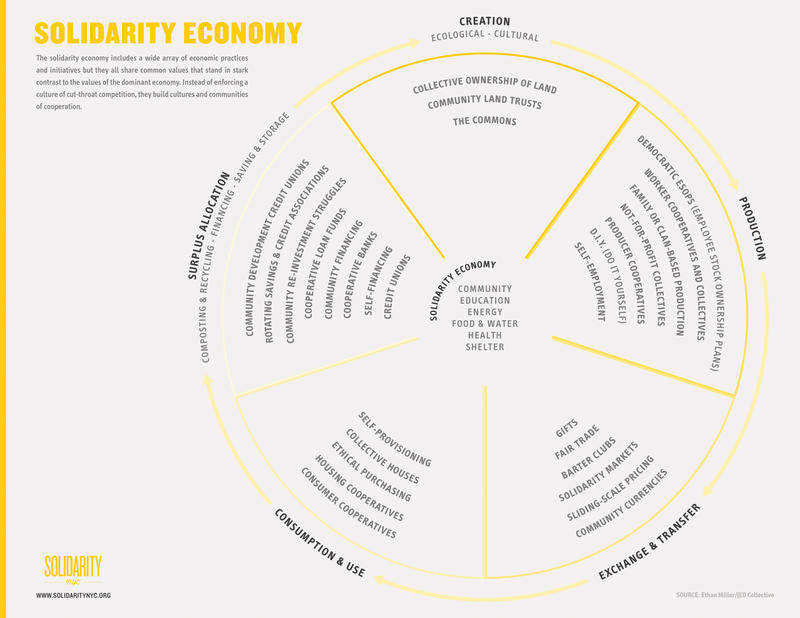
\includegraphics[width=.9\linewidth]{solidarity-economy.jpg}
	\caption{Economía solidaria.}
	\label{fig:solidarieco}
\end{figure}

Una economía tecnocrítica debería basarse en cadenas de producción que sean cíclicas y ecológicas, además de proponer trabajos orientados a la economía de la regeneración para generar empleos que restauren el medioambiente.

\begin{figure}[htbp]
	\centering
	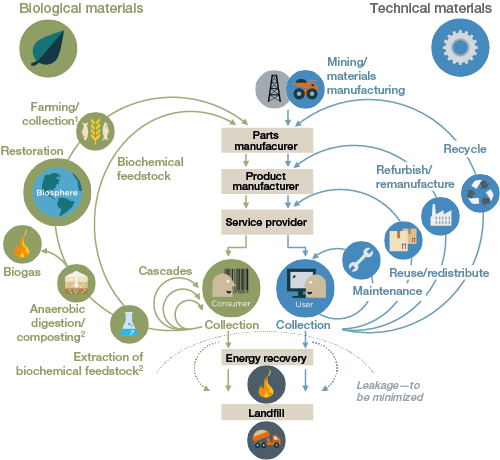
\includegraphics[width=.9\linewidth]{circular-economy.png}
	\caption{Economía circular.}
	\label{fig:circuleco}
\end{figure}

Frente a la falta de fundamentos teóricos de muchas propuestas políticas contemporáneas, nosotras creemos que el mundo donde caben muchos mundos se nutre de \emph{una ecosofía (un saber desde la Tierra), xenofeminista (que entiende las formas de opresión como el género, la raza o la clase social como tecnologías) e interseccional (que considera que distintas violencias se intersectan en las subjetividades)}. Es a partir de esta posición que tiene sentido para nosotras pensar una consideración estratégica sobre la práctica política. Hay que ir más allá de las adherencias identitarias a una facción política. Por ejemplo, la dialéctica entre horizontalismo y verticalidad es un falso dilema, ambas formas conviven en todas las relaciones grupales. Más allá de una nomenclatura en particular, nuestra posición siempre es tecnopolítica y busca prácticas anticapitalistas y antiestatales, creando comunes que permitan la gobernanza de grupos que pueden reapropiarse el valor del globalismo, descentralización, sociocracia, etc, entendiendo las subjetividades más allá del control administrativo central de la sociedad, es decir, de las normas que configuran los vínculos sociales.

La economía del don es parte de la visión de los comunes. Existen ejemplos como Grameen Bank que contribuyeron a terminar con la situación de pobreza de muchas personas en la India. Pese a que reproduce en cierto grado la lógica que las produce, sí logran generar un cambio de alto impacto. Es decir, escalable. Se trata de hacer modelos para descubrir, por ejemplo, cuántas vidas puede salvar tu proyecto, qué tan capaz es de visibilizar y crear alternativas a las violencias estructurales que sufre una persona, y encontrar proyectos clave que reduzcan transversalmente distintas formas de violencia al mismo tiempo, algo parecido al principio de Pareto.

El punto central de este apartado es señalar que la imaginación política presupone ciertas formas de hackeo a los dispositivos que dan fuerza a todo el embrujo mercantil, que son las formas abstractas de valor. El arte y el dinero tienen una relación importante en cuya génesis se pueden explorar algunas posibilidades de emancipación. La meta es reducir la dominación mercantil en estructuras económicas productivas.

\begin{figure}[htbp]
	\centering
	
\includegraphics[width=0.6	\linewidth]{artAfterMoney.jpg}
	\caption[Recomendamos el texto de Max Haiven.]{Recomendamos el texto de nuestro colega Max Haiven.}
	\label{fig:Haiven}
\end{figure}

\chapter{Principios para la acción efectiva}
\label{cha:principios}

Por ahora, frente a la acelerada decadencia de nuestros vínculos políticos, creemos que es necesario crear un ecosistema de tecnologías cívicas para hacer efectivas las garantías jurídicas a las personas ciudadanas que, por sus condiciones particulares, no pueden tener acceso a la justicia o al gobierno. Este movimiento tiene que luchar por una cultura pirata, es decir, concentrada en hacer libres, abiertos y accesibles todos los recursos de los que dispone. De la misma manera, necesitamos desarrollar principios de política pública, de economía y de gobierno, que se vuelvan el sentido común de tanto de las planificadoras como de las estudiantes de las escuelas de negocios y de administración. En cierto sentido, se trata de desarrollar un nuevo pensamiento económico que haga frente a la visión neoclásica de entidades racionales y maximizadoras de utilidades. En cuanto a nuestra estrategia, nos reconocemos en una tensión entre la transparencia y la opacidad. Sabemos que el humor juega un papel fundamental en la conformación de un nuevo imaginario político. Hasta ahora, hemos pensado en algunos principios como parte de una visión efectiva de la táctica política progresista:

\section{Pragmatismo no es utilitarismo}
\label{sec:pragmatismo}

Muchas personas casadas con la Teoría crítica (marxismos, psicoanálisis, etcétera) satanizan la filosofía del hacer efectivo y eficiente. Nosotras pensamos que esta actitud de repudio a la estadística, a la optimización y a la eficacia son lo que nos ha valido tantas derrotas. Podemos pensar las cosas más románticas del mundo sobre la revolución, pero la realidad es que toda operación requiere un pensamiento estratégico, requiere instancias (es decir, medios concretos de ejecución, como el código en computación) y que no lograremos disputarle el sentido común al neoliberalismo, ni imaginar un más allá del Estado o del capitalismo si no pensamos que teoría, estrategia y práctica están interrelacionados y que no bastan buenas intenciones. Como lo señala Alinsky en su Tratado para radicales, las cuestiones morales no tienen ningún sentido frente a nuestros enemigos. Ahí mismo señala que la historia nos ha enseñado que primero se toma la acción y después se legitima.

\begin{figure}[htbp]
	\centering
	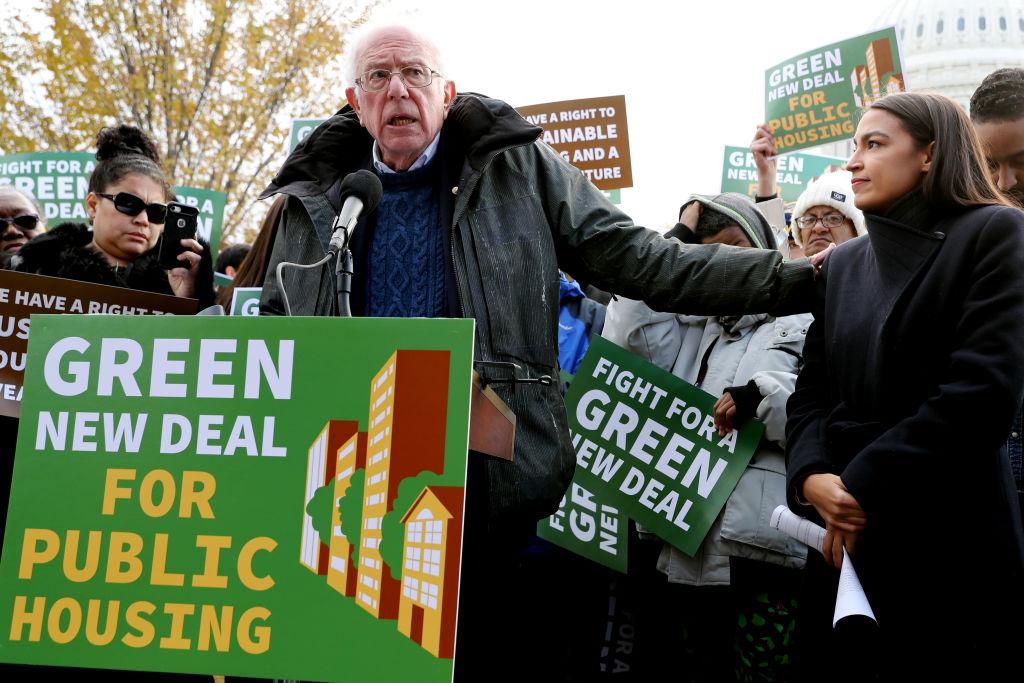
\includegraphics[width=0.9\linewidth]{green.jpg}
	\caption[Buen ejemplo de pragmatismo con sentido.]{Bernie Sanders, Alexandria Ocasio Cortés y el \emph{Green New Deal} son un buen ejemplo de pragmatismo con sentido.}
\end{figure}

\section{Interseccionalidad en la acción}
\label{sec:interseccionalidad}

Que todas nuestras acciones estén centradas en atender las condiciones estructurales de opresión a través de un movimiento emancipatorio que busque hacer frente de forma transversal a las diversas formas de violencia que padecen las personas. Para lograrlo, es necesario que entendamos cómo funciona el capitalismo hoy en día, en un contexto donde la fuerza de trabajo está totalmente precarizada, pulverizada y disuelta, en una época económica conocida como posfordismo, que consiste en una era donde la producción está profundamente ligada a la teoría de la información y de la computación. La interseccionalidad nos obliga a concentrarnos en desarrollar herramientas para comprender cómo funciona la explotación en sus distintas formas, por ejemplo, cómo se intersectan las violencias de género, racistas y de clase.

\begin{figure}[htbp]
	\centering
	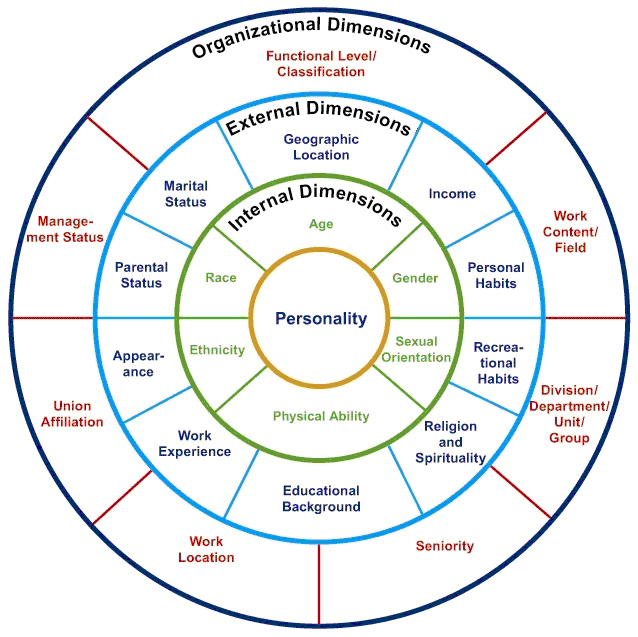
\includegraphics[width=\linewidth]{self-dimensions.png}
	\caption[Dimensiones de la personalidad.]{Dimensiones de la personalidad y factores de influencia.}
	\label{fig:dimensiones}
\end{figure}

\section{Transmisibilidad, o sea, hacernos accesibles}
\label{sec:transmisibilidad}

Si la ideología es el conjunto de significados culturales que nos hacen estar a favor o en contra de algo, necesitamos crear mecanismos de reconocimiento y traducción de estos significados para poder transformarlos. La mayoría de las personas no está realmente convencida de todo lo que cree y muchas veces lo cree más por ser receptora de un flujo de imágenes o de opiniones de gente con reputación social, que por su propio convencimiento. Ese es nuestro objetivo, ser capaces de comunicar a esas personas una visión comprensiva de la diferencia, de la otredad, de la dignidad del prójimo. Debemos hacer que nuestro discurso sea trans-ideológico, que pueda dialogar con distintas visiones reapropiándose y resignificando conceptos cooptados por conservadores y tradicionalistas (es decir, la derecha). Esta idea es parecida a lo que en ciencias sociales se conoce como intersubjetividad, que es la capacidad de las hablantes de crear significados comunes y compartidos que configuran su sentido común. Para lograr ser transmisibles, necesitamos más mercadotecnia para transmitir una cultura crítica y para comunicar el feminismo y la teoría crítica a gente que sabemos que podría accionar hacia una causa en particular, induciendo una disonancia cognitiva. Pensémoslo como si estas personas fueran \emph{swing voters} que tienen que elegir entre el sentido común neoliberal que las aliena o una visión crítica que las ayuda a reconocerse como personas con dignidad más allá de los códigos sociales. Pero no podemos hacer esto si no pensamos en los códigos de quienes nos escuchan. En el Corán, la \emph{taqiyya} o \emph{kitman} es el acto de disimular nuestras propias creencias en tiempos de persecución. Necesitamos disimular nuestras creencias y visibilizar mensajes seleccionado cuidadosamente para que logren insertarse en los flujos de deseo del capitalismo sin que el enemigo nos reconozca.

\begin{figure}[htbp]
	\centering
	
\includegraphics[width=\linewidth]{he4she.jpg}
	\caption[Emma Watson, vocera del \emph{He for She}.]{Emma Watson, vocera del \emph{He for She}, una forma de \emph{mainstreaming}.}
	\label{fig:he4she}
\end{figure}

\section{FLOSS y la bandera pirata}
\label{sec:FLOS}

En la jerga \hlfix{geek}{En cursivas.}, \emph{Free/Libre and Open Source Software} (FLOSS) es el tipo de software accesible a través de su código fuente. Esta filosofía es absolutamente necesaria para una práctica que permita el autogobierno de las personas y reduzca la dependencia al Estado y a los mecanismos tradicionales de gobierno, así como el poder de mercado de las corporaciones a través de las patentes. Nosotras añadiríamos \emph{Free/Libre and Open Source Culture} (FLOSC) para referirnos a un desarrollo en la cultura donde los procesos de creación de valor y de desarrollo de productos sean visibles y no ideológicos, es decir, que sirvan para que más gente pueda producir sus propios significados y sus propias estéticas y no para que sea utilizado para que la gente reproduzca un modelo de consumo (que es la función de la ideología). La cultura FLOS debe extenderse al espacio público, a la Academia, a los mercados (que hoy en día pertenecen a horribles lagartos que, a través de cinco empresas, controlan los flujos de distribución de mercancías y de imágenes en todo el planeta), a la educación y a todas las instituciones que reproducen el estado actual de las cosas. Esto significaría que el gobierno deje de operar empresas estatales y que más bien permita sus operaciones públicas, a través de certificaciones y procesos de descentralización, y no a través de la concesión a grandes monopolios transnacionales.\footnote{Entendemos, sin embargo, que hay problemas importantes cuando pensamos en proyectos que son intensivos en capital, como grandes obras de infraestructura o complejas investigaciones médicas. También se trata de acelerar los procesos de democratización y de FLOS dentro de la estructura de las corporaciones, que hoy en día, son reinos con el todopoderoso CEO (\emph{Chief Executive Officer} o director general) gobierna sobre todos sus súbditos a través del salario.}

Respecto a la cuestión de las patentes, hay ideas muy interesantes como el \emph{copyleft} o el \emph{copyfair} que buscan reformular patentes y crear esquemas que fomenten cooperativas. Nosotras pensamos que este tipo de prácticas podrían servir en las licitaciones gubernamentales para generar leyes que obliguen a las instituciones públicas a tener procesos y patrones de cultura FLOS.

Otra idea con la que hemos coqueteado es con las etiquetas o \emph{labels} en inglés. Por ejemplo, una etiqueta \emph{Low tech} que certifique que ciertos productos desarrollados fueron diseñados como alternativas a la obsolescencia programada y con la posibilidad de intervenir sobre ellos. La idea de la etiqueta surge como una forma de crear un sistema de certificados que pueda competir con la lógica capitalista de producción de las grandes marcas, con la intención de desacelerar los ciclos de producción y consumo.

Algunas referencias interesantes para complementar este apartado:

\url{http://unenumerated.blogspot.com/2017/02/money-blockchains-and-social-scalability.html}

\url{http://unenumerated.blogspot.com/2006/11/wet-code-and-dry.html}

\begin{figure}[htbp]
	\centering
	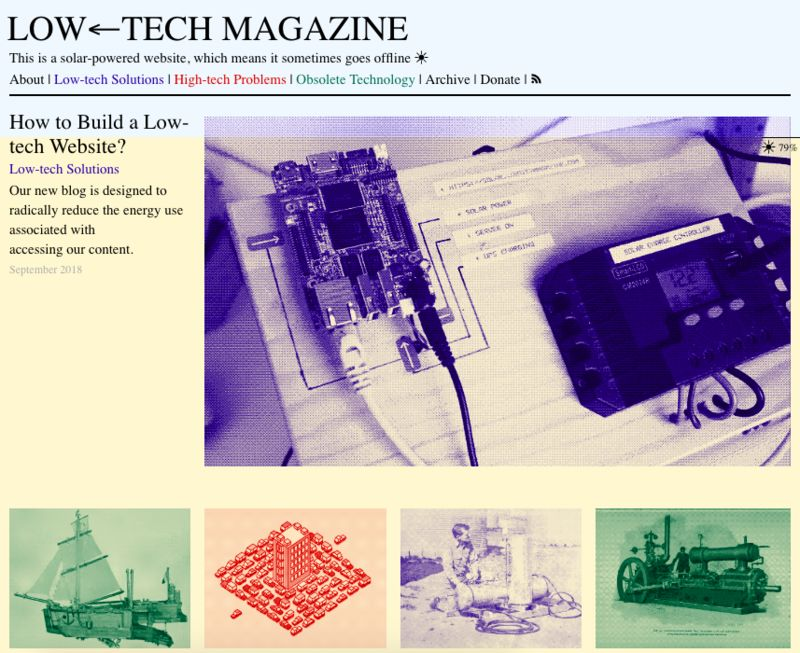
\includegraphics[width=.9\linewidth]{low-tech.jpeg}
	\caption[\emph{Low Tech Magazine}]{Imagen del sitio \emph{Low Tech Magazine}.}
	\label{fig:lowtech}
\end{figure}

\section{Queremos un mundo más allá de la economía capitalista}
\label{sec:mundo}

Algunas personas dicen que incluso si acabáramos con el capitalismo como forma de explotación, todavía habría que pensar en cómo ir más allá de relaciones sociales mediadas por abstracciones como la moneda. ¿Por qué? Cada vez presenciamos cómo hasta la última esfera de la vida está sujeta a la regulación, a la medición y a la cuantificación. Esto nos impide vivir sin considerarnos a través de márgenes de utilidad y hace que nos sigamos mirando las unas a las otras, al menos parcialmente, como objetos de interés. La cibernética es la ciencia y arte del control que cuantifica cada vez más toda experiencia de vivir en \emph{clicks}, en \emph{shares}, en \emph{likes}, y esto no hace sino aumentar el deseo de enjuiciarnos cada vez más. Una posible solución está en pensar que las tecnologías que desarrollemos para crear un Estado más justo también tienen que preguntarse cómo haremos para generar más vínculos, más encuentros donde las personas puedan hablar, escucharse y establecer vínculos más allá de la pertenencia a una tribu identitaria o a cualquier grupo de interés. Creemos que el verdadero problema de la tecnología es su desarrollo capitalista, que desorganiza a las personas para volverse cada vez más necesaria.

Para lograrlo, podemos valernos de investigaciones como \emph{Nudge economy}, parte de la economía de la conducta que analiza el diseño de incentivos que conducen a la gente a tomar decisiones, es decir, la disposición económica de los objetos a las personas. En este campo es también posible vincular la experiencia de usuario o UX (\emph{user experience}) para hacer interfaces más accesibles e incluso más comunitarias.

\begin{figure}[htbp]
	\centering
	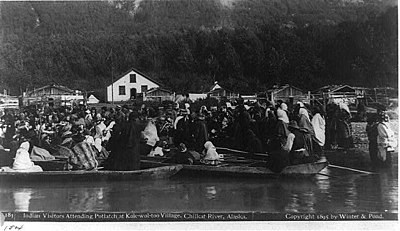
\includegraphics[width=\linewidth]{potlatch.jpg}
	\caption[\emph{Potlatch}.]{El \emph{potlatch}, concepto clave en la economía del don de Marcell Mauss, es un ritual de los pueblos aborígenes de la costa del Pacífico en el noroeste de Norteamérica, tanto en los Estados Unidos como en la provincia de la Columbia Británica de Canadá. EE.UU.}
	\todo[inline]{Corregir el brillo y contraste de la imagen para que se pueda ver con más claridad.}
	\label{fig:potlatch}
\end{figure}

\section{Luchemos por estar en los canales masivos}
\label{sec:luchemos}

El algoritmo del capitalismo funciona implantándonos deseos de consumir y de cumplir ciertos códigos sociales que siempre tienden al individualismo y a la mercantilización de las otras personas. No creemos en la falsa dicotomía entre luchas locales y globales, creemos que hoy en día, toda forma de activismo es una cierta tecnopolítica. Es decir, que nuestras prácticas contienen cierta posición estratégica sobre el uso de los recursos en decisiones tan básicas como usar manuales de \emph{zero waste} en eventos públicos y hacer campañas para hacerlo una moda. Si realmente queremos hacer algo efectivo, tenemos que crear un \emph{mainstream} o corriente mayoritaria que permita unir distintos proyectos que luchan por la emancipación así como los ingleses tienen BBC como distintivo de su identidad y de su cultura.

El trueque, el \emph{freeganism} o los bancos de tiempo son estrategias de resistencia que por sí solas, aisladas en contextos locales, de micropolítica, no pueden hacer nada para ganarle a los millones de dólares que la industria de la comida rápida invierte en hacernos desear el azúcar, las grasas y cualquiera de esas sustancias que nos restan salud. Sin embargo, combinadas en una campaña masiva y consolidando audiencias que puedan encontrar alternativas sistémicas como salud pública y comedores comunitarios, empezaremos a tener victorias reales. Es decir, hay que crear flujos alternativos a la cultura de masas que tengan aspiren a una plataforma común de organización, para hacer publicidad no a un proyecto de bajo impacto en particular, sino a una alternativa sistémica y escalable. Para nosotras, Wikipolítica fue la muestra de que tenemos la capacidad de hacer funcionar una maquina capaz de hacer campanas de mercadotecnia con alcance nacional que lleguen a diferentes segmentos e incluso lleguen a medios masivos internacionales.

\section{La crítica debe enfocarse en las tecnologías que producen la opresión}
\label{sec:critica}

Nuestro discurso debería ser interseccional e incluir en su agenda un conjunto de propuestas sistemáticas en torno a cada lucha particular. En la dinámica actual del capitalismo, hacer uso de las marcas puede darle más poder a la lucha. Necesitamos crear una red para consolidar, para entablar puentes de colaboración de saberes técnicos. Es importante mencionar que en la cooperación técnica se pueden hacer progresos discursivos paralelos, una identidad mínima interseccional, un vínculo común de articulación para la comunicación estratégica de una red de círculos que construyan una plataforma con procesos y patrones en común para incentivar la participación política.

Se nos ocurre que incluso sería buena idea hacer campamentos de inteligencia colectiva. Estos deberán operar a través de la escucha y plantear preguntas de empatía: ¿cómo se sienten hoy? ¿Cuál fue tu logro más importante de esta semana? ¿Qué problemas hay en la organización? ¿Qué respuestas podemos crear desde nuestra posición para solucionar el problema? ¿Cómo se sintieron con esta dinámica? Nos imaginamos talleres diversos, como educación popular, herramientas de mapeo, el buen trato como estrategia de lucha, participación ciudadana, herramientas filosóficas, lluvia de ideas y dinámicas de inteligencia colectiva para una cartografía de controversias.

Hoy en día es posible desarrollar la economía social para tratar de enlazar distintos proyectos de resistencia, basados en estructuras de micro mecenazgo. El horizonte educativo podría ser una cruzada contra el analfabetismo digital, con la intención de que todas las personas puedan navegar en la complejidad de la era de la información.

\chapter{La organización que construimos}
\label{cha:organizacion}

\section{Sobre el asunto de la estrategia y la táctica}
\label{sec:tacticaestrategica}

Los principios de una organización deben combatir el capitalismo a diferentes escalas, refiriéndose a la otra persona, a los grupos de personas y al propio cuerpo. Antes habíamos señalado que las formas de opresión tienen manifestaciones macro y micro, que bien pueden entenderse como globales (o económicas, sobre el acceso a los recursos y a los mercados) y como locales (o corporales, sobre las convenciones sociales que rigen nuestra vida cotidiana). De un modo parecido, la acción política puede entenderse desde dos aristas que se entrecruzan: la estrategia, la táctica y la organización. La estrategia atañe a lo global, a las grandes estructuras que dan forma a las interacciones económicas a escala masiva mientras que la táctica se refiere a los detalles de implementación para grupos concretos, a nivel local. Si lo pensamos en relación con un partido político, las estrategias tienen que ver con el desarrollo de un programa política, un plan de gobierno y la creación de un horizonte de acción mientras que la táctica está más relacionada con las acciones concretas que nos llevarán a la victoria, como ganar una elección o el cabildeo para pasar una ley a través de litigio estratégico e intervenciones mediáticas.

Sin embargo, hasta ahora no queda tan claro cómo interactúan la estrategia y la táctica. Es ahí donde entra el rol de la organización.

Para crear una fuerza política que vaya por la toma del poder, tenemos que construir un plan de gobierno deliberado al que tienda el sistema de partidos basado, entre otras cosas, en la noción de soberanía tecnológica.\footnote{Un ejemplo de esto serían los incentivos a proyectos antimonopólicos, protocolos y librerías de acceso público para que cualquiera pueda entrar a la economía formal y tener acceso a servicios de calidad por parte del Estado.} La tarea es crear una plataforma global que nos permita organizarnos mejor como un todo, darle mayor poder a nuestras luchas como una confederación de colectivos o algo así. Esta tarea no es sencilla y descansa, en última instancia, de la confianza que exista en las otras, todo el tiempo. Para hacer frente a ello, necesitamos salir a la calle y ahí está el gran acierto de Wikipolítica, en salir a tocar puertas. Salir a la calle es abrirnos, es dar vida a un movimiento social que, entre otras cosas, tome las elecciones populares como una oportunidad de articulación. Lo federal solo es necesario en la medida en que apoye una agenda local, estrategia electoral municipalista. Dentro de nuestro programa político está la urgencia de abrir hasta el último dispositivo que perpetúe, bajo la servidumbre, un grado de opresión tal que imposibilita que una vida particular no pueda desarrollarse como potencia.

Para hacer una opción electoral fuerte necesitamos crear una propuesta integral de gobierno que sea capaz de integrar diversas agentes y una maquinaria electoral que garantice la fiabilidad de las representantes. Muchas activistas no tenemos idea de cuáles son los retos cotidianos de la vida real, de la gente. Nuestra idea de un cambio estructural tiene que ver, precisamente, con afectar las estructuras que generan opresión sistemáticamente para la mayoría de las personas.

Para quienes disputan los puestos de representación, hay que tener muy claro que las campañas electorales son un proceso, no un fin en sí mismo. Antes de pensar en elecciones, es importante que los grupos políticos se pregunten cómo conformar una base social que sea capaz de producir flujos de interconexión, como el mostrado en el diagrama 2.1\todo{¿y ese cuál es?}. Por ahora, sin estructuras políticas suficientemente inteligentes y resilientes, hay que promover la operatividad de todas las organizaciones pensándolas como entidades completas cuya primera tarea es garantizar la subsistencia y las necesidades mínimas (como las señaladas por Maslow en su famosa pirámide de necesidades) permitiendo que haya distintos proyectos que generen recursos propios, pero que gocen de una membresía común que les ayude a organizarse y a conectarse con otras redes de resistencia y colaboración. Para lograrlo necesitamos implementar operaciones de inteligencia sobre el tráfico de la red, entender de qué modo, bajo qué significantes, opera el \emph{statu quo}. Es decir, cuáles son los conceptos que están en disputa para llevar nuestra visión de cómo \emph{nos} gobernamos en dirección no sólo a las urnas, sino a la calle, a la acción cotidiana.

A diferencia de un partido, que opera bajo la lógica de competencia de un sistema que busca ganar, un movimiento social puede permitirse crear, conectar y estructurar esfuerzos paralelamente e incluso al interior de los partidos, señalando los problemas fundamentales de éstos en función de un marco teórico deliberado entre bases, sociedad civil, intelectuales y artistas, y proponer soluciones a esos problemas. En este caso hipotético en el que, después de la deliberación, existiera un proyecto político claro y deliberado por diferentes sectores, los partidos que desearan sobrevivir tendrían que limitarse a ejecutar las metas trazadas por los distintos grupos, y representadas bajo una agrupación de medios de comunicación. En este sentido, el gobierno y el sistema de partidos perderían buena parte de su poder doctrinario para limitarse a cumplir funciones meramente técnicas. Para hacer una transformación histórica, necesitamos ser un espacio de encuentro entre academia, sociedad civil, empresarios, medios, sindicatos, organizaciones de base y opinión pública. Concentremos nuestros esfuerzos en hacer que la agenda sea un conjunto de compromisos a largo plazo ---junto con nuestras líneas de acción--- mientras conformamos un proyecto político bien organizado y con plataformas tecnológicas chidas.

\begin{figure}[htbp]
	\centering
	\includegraphics[width=.9\linewidth]{spheres-practices.png}
	\caption{Interacción entre prácticas electorales, teóricas, mediáticas y de calle.}
	\label{fig:interacciones}
	\todo[inline]{Valdria la pena rehacer un diagrama como este en español.}
\end{figure}

Una vez que logremos consolidar una infraestructura común y dinámicas para comunicarnos, es necesario que abramos canales de comunicación. Para lograrlo, podemos recurrir a estrategias muy antiguas, pero igualmente efectivas bajo una gran organización técnicamente capaz de hacer una democracia efectiva: Periodismo popular, repartido en lugares de resistencia a través de estructuras distribuidas por todo el país, donde los contenidos puedan enlazar realidades locales con la nacional. En realidad, la presencia de una organización política en el territorio no significa que haya buenas razones para ocuparlo, la razón por la que nos presentamos en la calle es quizá una de las cuestiones más importantes a resolver. Por ejemplo, adoptar una agenda municipalista sería un excelente horizonte para un movimiento que busca ocupar las instituciones del poder. Las propuestas de Murray Bookchin, ecologista estadounidense, pueden convivir con otros esfuerzos de organización comunitaria como los desarrollados por Saul Alinsky y Marshall Ganz. Quizá la razón más vital para salir a la calle sea la más poderosa. El carnaval, la festividad profana de lo público, la danza libre y el encuentro de los cuerpos, sería un gran pretexto. ¡Salgamos a la calle a divertirnos y hablar de lo político! También puede servir para redefinir nuestra concepción de un mercado libre y abierto.

Se pueden conciliar movimiento y elecciones a través de participación escalonada que se gestione a través de una plataforma web, así como plantear acciones importantes pero no urgentes para la organización y para desarrollar el movimiento. Esto para hacer una mancuerna operativa con las personas que consideran que conquistar espacios de poder es la tarea urgente, pero que estarían de acuerdo con abrir la organización para que estas acciones importantes empiecen a ocurrir porque somos una wiki inteligente, que entiende el aspecto multidimensional de sus operaciones. Imaginamos una apertura escalonada de información, según lo que la gente quiera compartir y lo que la wiki haya ganado por su mérito de honorabilidad. \emph{Hay que entender que hoy es posible programar la gestión de responsabilidades orgánicamente.} Las alianzas deben permitirnos articular una red electoral, un plan de gobierno y un nuevo proyecto constitucional, desde una perspectiva abierta, transparente y \emph{FLOSS}. Consideremos que hay una asimetría en acceso a redes que hacen que gente menos experta o que ha pasado menos tiempo en la red tenga mayores dificultades para integrarse. Por esta razón no sabemos dar cauce a muchas ideas que son potencialmente grandes proyectos. Más allá de la preocupación, porque un grupo de poder coopte la organización, hay que pensar que es necesario que el movimiento se fragmente y diferencie a partir de recursos comunes, bajo una visión modular y escalonada de los progresos de nuestra estructura política.

\begin{figure}[htbp]
	\centering
	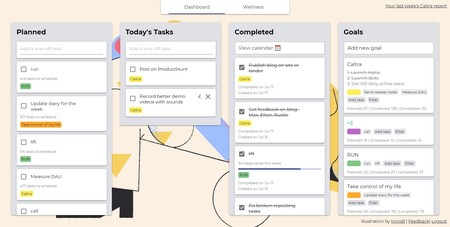
\includegraphics[width=.9\linewidth]{caltra.jpg}
	\caption{El sitio \url{www.caltra.co} te permite organizarte en listas y tableros.}
\end{figure}

El problema de la documentación de un movimiento político que busque la libertad real de todas las personas es una preocupación muy presente desde Podemos, pero realmente constante a lo largo de la historia. El problema más importante hoy en día para los movimientos autogestionados se conoce como la \emph{tiranía de la no estructura.} Un problema difícil de enfrentar es que, en relación con el estado actual de las cosas, solo podemos ver lo que nos queda y muy pocas veces lo que nos ha sido arrebatado o todo lo posible, un horizonte imaginario de formas de organización, de diálogo, distintas. La cuestión de la inteligencia colectiva no puede quedarse como un instrumento más para agilizar la productividad. Mucha gente en Wikipolítica no se da cuenta lo útiles que resultan al Imperio con el burdo aceleracionismo de blancos por el que sienten tanta simpatía. Para hacer frente a estas cuestiones, necesitamos mecanismos para profesionalizar el activismo y la militancia, mecanismos de sistematización de experiencias. Partir de esto para diseñar un programa de crecimiento dirigido, comprensivo y estratégico, una suerte de comunidad de inteligencia. Tenemos oportunidad de usar y desarrollar plataformas tecnológicas para gestionar procesos que ahora son inoperables bajo la tecnología que tenemos ahora. Para lanzar una campaña de crecimiento dirigida al territorio necesitamos despliegues de profesionales en Trabajo social en Comunicación. Es decir, necesitamos pensar estratégicamente. El problema es que entre muchas personas es moralmente incorrecto repetir

En Wikipolítica muchas veces nos preguntamos sobre las características de un posible espacio wiki oficial. Con el tiempo, estamos más convencidas que se trata de plantear qué significa un espacio wiki, preguntarnos cómo inspiramos a otras personas a crear espacios bajo una filosofía común. La ideología es la máscara a través de la cual vemos las cosas.

El diseño es parte de una propuesta de inteligencia que, a través de procesos de iteración y prueba, logra crear relaciones de experiencia entre las cosas y las personas. Creemos en el valor del Diseño como disciplina fundamental para la transmisión de un medio popular. Nuestro \emph{código} tiene que pensar en las instituciones a través del Diseño social. El resultado será mecanismos que incentiven la participación más allá de la lógica utilitarista, fundamento de la magia negra. La única restricción serían las manifestaciones de totalitarismo, como la intolerancia, el autoritarismo o la intransigencia. Los discursos que atenten contra la determinación libre y voluntariosa de la persona deben ser contenidos y este es un límite al que no estamos dispuestas a renunciar.\footnote{El mejor remedio para los fascistas de sonrisa cínica y espíritu perverso es molerlos a palos. Pero nos conformamos con que sean expulsados.}

Por ejemplo, aprender a pensar en instancias para crear protocolos comunes de distintas luchas como las tecnologías de \emph{performance} o la táctica del brigadeo. Operaciones orientadas a proyectos, donde las estructuras nazcan y mueran, sean ocupadas, como los hackerspaces. Metodologías de organización para y desarrollo para personas como SCRUM, design thinking, UX, grupos de agilismo, Workcafé. Otra tarea es consolidar un equipo de relatores que puedan sistematizar con rigurosidad los resultados de todas las discusiones, pues parece que la relatoría presupone más habilidades para la síntesis y la estructuración discursiva de lo que podría parecer.

La cuestión de una plataforma política puede funcionar muy bien como un proyecto modular de fuentes libres y abiertas basado en tecnologías que ya existen, como Decidim y las metodologías de gobernanza en círculos llamada Sociocracia. Con esta visión es muy factible desarrollar una estructura informática con directorios, sesiones de planificación y estrategias de mercado, asesoría para participar en convocatorias y solidaridad para que quienes quieran, se apoyen. Solo habría que considerar que el crecimiento esté dirigido estratégicamente hacia redes y personas clave en agendas específicas, además del mero crecimiento territorial. Necesitamos comprometernos con sentar un precedente operativo basado en nuestro potencial tecnológico. Si lo hacemos bien, la necesidad de apertura de otras asambleas políticas en el país se esparcirá como un meme (virus cultural), que permita que todas tengamos los saberes necesarios para organizarnos en torno a lo común.

En términos estratégicos, es mejor dar un golpe nacional de la nada, con precisión y organización, con artistas, académicos, opinión pública y otros sectores, que el desgaste que implica concentrarse en un solo proyecto de corto plazo, como una campaña política o una petición legislativa sin ninguna repercusión estructural. Mejor esperar unos años hasta que tengamos una organización poderosa. Abrir la organización con un movimiento nacional que siente las bases para un proyecto político fuerte y de larga duración.

Representación de convicciones políticas, agendas desde subjetividades reconocidas y desde los territorios. Burocracia media en sindicatos o partidos. Diferencia y relación entre sindicatos y partidos. Redes interuniversitarias. Necesitamos regulación de proyectos económicos a través de sus limitaciones. Es decir, si la industria editorial genera capital que se acumule en pocas manos (lo que significa menores ingresos tanto para escritorxs como para lectores), ser el espacio y respaldo de la innovación de nuevos modos de financiamiento, quizá haciendo hackatones o dando prioridad al tema en las agendas de un período y una región en particular. Hackatones sociales o alguna iniciativa donde podamos ser facilitadoras de distintos fondos públicos locales. En el terreno económico podemos jugar el papel de gestoras para cooperativas de consumo que compartan una identidad y principios wiki que permitan que muchas familias puedan empezar a adquirir sus bienes en redes sororas.

\section{¿Cómo entender los problemas de nuestro país?}
\label{sec:problemaspais}

El Estado en México es un orden social de acceso limitado, hay que
pensar en systems thinking para crear un \emph{frame} que comprenda necesidades
para ajustar la plataforma política al contexto de institucionalidad y
reglas del juego propias de cada arreglo. Habría que partir de una
visión combinada de psicoanálisis, diseño y economía de la conducta. Hay
que hacer una lista de problemas principales a resolver, por ejemplo:

\subsection{Problemas de diseño de sistemas:}
\label{sec:probsis}

\begin{itemize}
	\item Interfaces y experiencia de usuario comunitarias y accesibles

	\item Teoría del empujón para incentivos económicos a cooperativas y apropiaciones comunitarias del espacio público
\end{itemize}

\subsection{Problemas de acción colectiva}
\label{sub:probaccion}

\subsubsection{Económicos}
\label{subs:economicos}

\begin{description}
	\item[Asimetrías de información:] cómo hacemos que la gente tenga los mismos insumos para tomar las decisiones más benéficas para las comunidades en un mercado complejo de transacciones en tiempo real

	\item[Problema del agente-principal:] abolir las altas tasas cobradas por coyotes que dan sentido a la figura del Estado como recaudador central que redistribuye el ingreso

	\item[Tiranía de la no estructura:] sistemas de toma de decisiones para la participación escalonada y remunerada de diferentes agentes con un objetivo común de solidaridad económica

	\item[Comunes:] formalización en protocolos y procesos de una cultura de los bienes y servicios comunes que se gestionan, se actualizan y se mantienen a través de contribuciones preestablecidas en contratos inteligentes
\end{description}

\subsubsection{Psíquicos}
\label{subs:psiquicos}

\begin{description}
	\item[\emph{Schadenfreude}:] cómo crear grupos de personas con adicciones, resentimientos o comportamientos tóxicos que sienten placer por el sufrimiento del prójimo, y comenzar procesos de sanación colectiva descentralizados, como Alcohólicos Anónimos.

	\item[Narcisismo de las pequeñas diferencias:] Construcción de una cultura política que procure las alianzas y permita canalizar los disensos. Un ejemplo muy claro para la construcción de organizaciones que hagan frente a este tipo de cuestiones es la Sociocracia.
\end{description}

\begin{figure}[htbp]
	\centering
	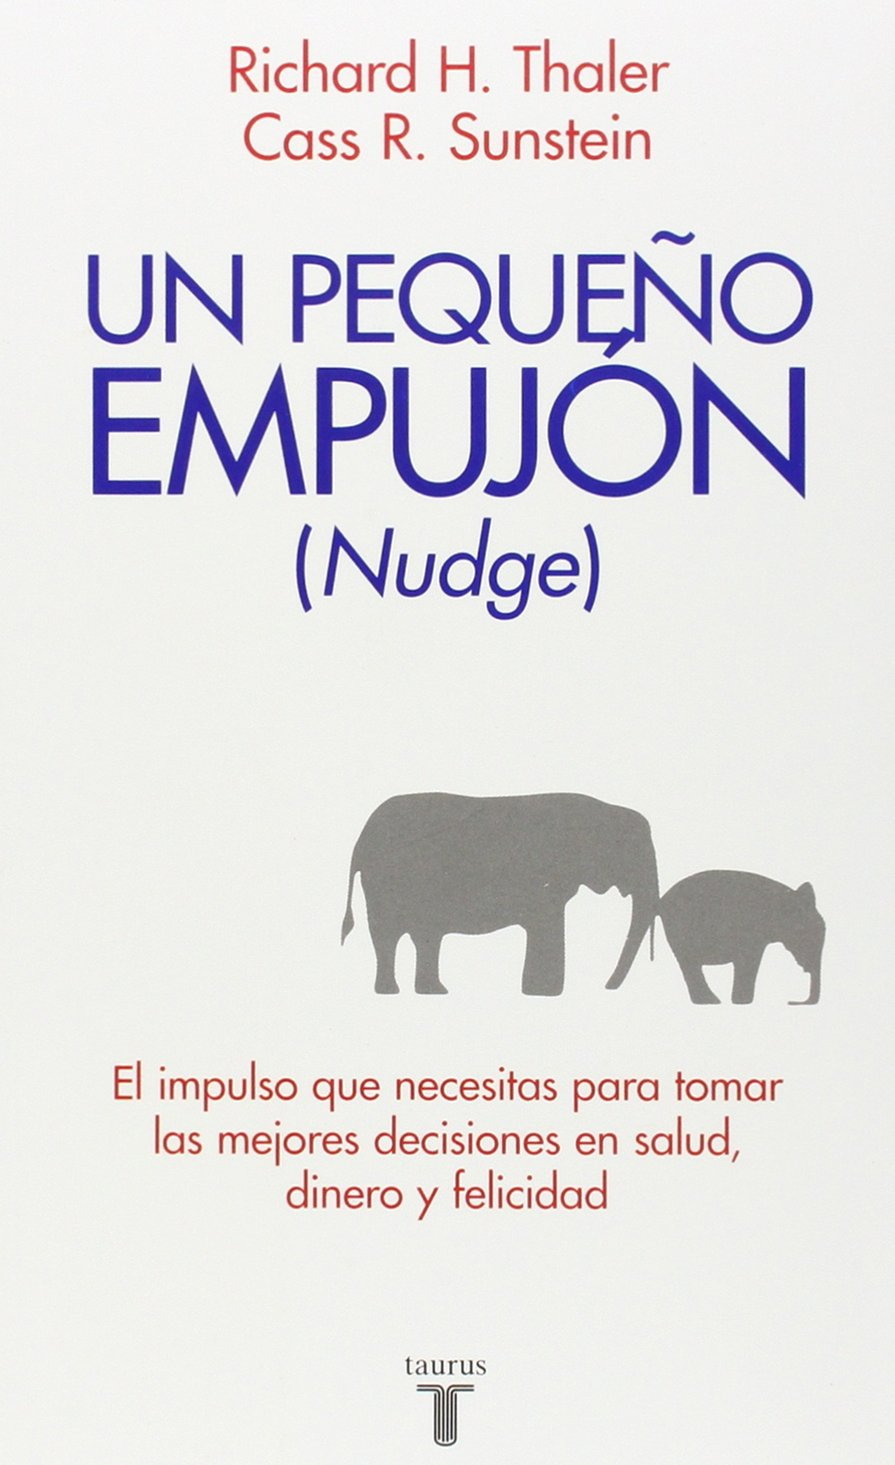
\includegraphics[width=.7\linewidth]{nudge.jpg}
	\caption[\emph{Nudge}]{El libro \emph{Nudge} es una gran referencia para entender el poder del diseño y la economía del comportamiento en la solución de problemas públicos.}
	\label{fig:nudge}
\end{figure}

\section{Consideraciones sobre la organización}
\label{sec:considerorga}

Las herramientas ya existen, es poco trabajo en interconectarlo (compatibilidad de tecnología), hay que enfocarnos en la adopción a través de talleres y eventos de accesibilidad, de editorializar una base de datos opinionated suite de trabajo militante), de garantizar protocolos de seguridad: decentralizacion, permisos (gestión de identidad) (Pursuance, sneakernet y otras tecnologías). Tenemos que desarrollarlo poco a poco a través de una arquitectura modular y distribuida, que permita ensamblar diferentes tecnologías según las necesidades de la persona usuaria.

El problema principal para un movimiento horizontal es el problema de la \emph{no-estructura}. Dentro de las estrategias, podemos proponer visiones para que los emprendedores entiendan como disruptivo lo que es estructural. Se trata de reapropiarse del concepto de \emphh{gobernanza} dinámica y participativa, pensar que sea una gobernanza basada en \emph{outputs} o resultados sin que se vuelva una cosa individualista de \emph{tracking} de \emph{performance} individual. El objetivo es crear una estructura de los comunes (Elinor Ostrom), además de fortalecer sindicatos, acelerar cooperativas y democratizar decisiones corporativas, facilitar \emph{self-management}y \emphh{self-organization} en un movimiento \emphh{antileadership}.

Para lograrlo hay que retomar la paradoja de la sistematización de actividades ¿creamos y documentamos procesos o patrones? ¿Realmente vale la pena un modelo de gobernanza como sociocracia?

Recursos interesantes para este apartado:

Github: The GitHub Debacle and Why Holacracy is Bullshit
(counter-response)
\url{http://cbracy.tumblr.com/post/79876957198/the-github-debacle-and-why-holacracy-is-bullshit}

\chapter{¡Accionemos!}
\label{cha:accionemos}

¿Qué podemos hacer? Nuestra posición es una práctica pragmática y eficaz desde el xenofeminismo como filosofía de inspiración de La Partida. Más allá de la coherencia moral, nos interesa agruparnos con formas de vida que nos hagan potentes, es decir, en las formas de vida que procuran el cuidado, el bien común. Por ahora, con nuestra agencia limitada por la poca credibilidad de la juventud, nos toca infiltrarnos e incidir en diferentes medios, en partidos políticos, organizaciones internacionales, medios de comunicación masiva y segmentada, entre otras estructuras.

\begin{figure}[htbp]
	\centering
	
\includegraphics[width=0.9\linewidth]{leo-silvestri.jpg}
	\caption[Leonor Silvestri]{Leonor Silvestri, feminista argentina y activista de los afectos alegres con excelentes reflexiones en YouTube.}
	\label{fig:silvestri}
\end{figure}

\section{Algunas posibles acciones estratégicas}
\label{sec:posiblesacciones}

Un Centro de Estudios que brinde a las personas que estudian ahí capacidades de formación en medio de la complejidad y que formen generaciones dispuestas a accionar desde una perspectiva transdisciplinaria y colaborativa, lejos de los dogmas y formalismos de la academia. Como el proyecto de Nick Srnicek con Hellen Hester, autonomy.work. Dentro de los proyectos claves vemos:

Un \emph{think tank} para generar líderes con conciencia crítica, de estrategia y táctica política, además de informes de política económica de desarrollo local y estrategias para hubs y hackatones, además de programas de litigio estratégico rumbo a la creación de un programa de políticas publicas poscapitalista. Necesitamos crear lazos con los entornos tecnológicos progresistas y radicales para poder crear productos accesibles en los mercados que puedan generar bienestar para muchas personas, por ejemplo, a través de franquicias cooperativas.

\begin{figure}[htbp]
	\centering
	
\includegraphics[width=0.9\linewidth]{autonomyWork.png}
	\caption{Logo del \emph{think tank} comenzado por Hellen Hester y Nick Srnicek, \texttt{autonomy.work}.}
	\label{fig:autonomywork}
\end{figure}

Ademas, necesitamos crear una plataforma de organización política en línea de arquitectura modular que sea accesible y fácil de implementar. Un excelente punto de partida es el proyecto Decidim desarrollado en el MediaLab en España. Nos imaginamos las bases de una interfaz para discusión y gestión democrática de grupos, además de una wiki que funcione como un repositorio copyfair editorializable. Ademas, con tecnologías de georreferenciación.

En términos económicos, hay que crear un ecosistema que facilite la proliferación y producción de redes solidarias. Más allá del movimiento sindicalista, la cooperativa es una unidad económica que realmente garantiza la igualdad democrática desde el trabajo. Quizá la forma más sencilla de hacerlo sería a través de una franquicia cooperativista cuyo soporte sea una wiki con manuales y procesos accesibles en términos de diseño, que crezca bajo una etiqueta (\emph{label}) que represente los valores de esa marca cooperativa.\footnote{Un ejemplo del crecimiento rizomático de una organización es la nevería mexicana La Michoacana.}

Finalmente, es necesario desarrollar un proyecto cultural transmedia que funcione a través de esta lógica y que permita el desarrollo de una cultura popular independiente del mercado \emph{mainstream}. Algo de inspiración para una aventura de esta naturaleza han sido los \emph{Street papers} y proyectos como la Red de Producción y Distribución Vicente Guerrero en México, el manifiesto del Dogma 95 y el formato de producción de bajo costo desarrollado por Robert Rodriguez en su famoso libro \emph{Rebel without a Crew}. En resumen, una cultura de producción \emph{guerrilla cinema}. Las películas \emph{Tangerine} en Estados Unidos y \emph{Oso Polar} en México son una muestra de las posibilidades técnicas de los medios contemporáneos. Sin embargo, el horizonte de un esquema de producción audiovisual militante es ContraPoints, un vlog en YouTube estelarizado por Natalie Wynn.

\begin{figure}[htbp]
	\centering
	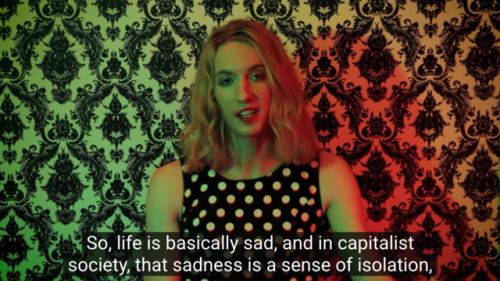
\includegraphics[width=.9\linewidth]{contrapoints.png}
	\caption[Natalie Wynn.]{Natalie Wynn, creadora de ContraPoints.}
	\label{fig:Wynn}
\end{figure}


\section{Organízate e independízate del Capital}
\label{sec:independizate}

Finalmente, lo más importante es encontrar la forma de compartir recursos que nos permitan crear redes de solidaridad en la producción de insumos clave para cubrir necesidades básicas de grupos y comunidades. En un sentido meramente estratégico, la pirámide de Maslow nos da pistas de las industrias que habría que comenzar a cooperativizar para crear multitudes que se emancipen de los flujos farmacopornográficos, chatarrofágicos y financieros que produce el capitalismo.

\begin{figure}[htbp]
	\centering
	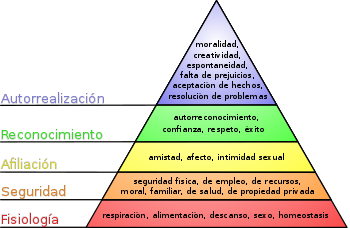
\includegraphics[width=.9\linewidth]{maslow.png}
	\caption{Pirámide de Maslow sobre necesidades.}
	\label{fig:maslow}
\end{figure}

Económicamente, problemas como el hambre o la vivienda pueden resolverse con técnicas avanzadas de planificación y coordinación que no podían realizarse en el socialismo de hace casi un siglo por la sencilla razón de que no contaban con las herramientas computacionales necesarias para poder pensar con seriedad en una economía planificada que publique precios y soluciones conflictos de asimetrías de información en el mercado.

Hoy tenemos la capacidad de no solo permitir la proliferación organizada en plataformas comunes de productoras descentralizadas que surtan en función de necesidades y no de plusvalía financiarizable, también podemos implementar sistemas de votación para que estas organizaciones no sean, como lo fueron durante la revolución mexicana, la base de un corporativismo de corte charro. Podemos crear plataformas de economía solidaria capaces de gestionarse autónomamente a través de recursos iterativos de código FLOS. En ese sentido, una etiqueta de franquicia cooperativa sería una buena forma de crear documentación y procesos comunes en un proyecto de riesgo compartido con un contrato claro e incluso inteligente y encriptado.


\part{Sobre la Acción Crítica}
\include{3-accion-critica/00-cite}
\chapter{Introducción: La neorreación devela la crisis del Estado moderno}
\label{cha:la-neorreación-devela-la-crisis-del-estado-moderno}

\epigraph{\enquote{Bajo tal mirada esta época nuestra puede ser llamada \enquote{época de ilustración} o también \enquote{el Siglo de Federico}}}{\emph{Immanuel Kant} en~\autocite[p.~11]{kantQueEsIlustracion2009}.}

Nuestro tiempo es de implacable ironía y de un cinismo cada vez más vacío. Mientras el proyecto de la Ilustración, gran promesa de los fundadores del Estado moderno, se derrite, las resistencias se refugian en formas de activismo poco capaces de transformar la realidad a escala molar, global. \footnote{Estos conceptos se refieren a una escala local, micro y global o macro, respectivamente Desde el vocabulario deleuziano son denominaciones comunes a este aparente binarismo.} La derecha alternativa llama a estos refugios de autocomplacencia \enquote{Catedrales}, un espacio seguro para el sentimentalismo y la camaradería de las minorías, incluyendo a una que otra persona que goza del estatuto verdadero de ciudadana y que deserta para alcanzar el \emph{tiqqun}, la redención. Los mismos hombres-masa resentidos llenan internet de propaganda que toma partido por la Ilustración tal y como la entendía el despotismo ilustrado de \enquote{hombres de Estado} como Federico el Grande.

Mientras, cualquier intento de imaginación política ha sido cooptado por el neoliberalismo, un momento histórico del capital donde el mercado tiene un producto para complacer a cualquiera. El desarrollo de la cibernética y el creciente poder de las corporaciones como entidades transnacionales inunda a cualquier discurso político de un montón de limitaciones económicas por un hecho fundamental: mientras las estructuras tecnológicas sean dominadas por la lógica privativa del capital, nunca será posible encontrar un afuera a la religión de Estado, pues la tecnología no solo condiciona nuestras capacidades tecnomateriales sino que también captura nuestro deseo e inunda nuestra avida psíquica.

En la \emph{Introducción a la guerra civil}, el Comité Invisible señala que la guerra civil es el libre juego de las formas de vida, el principio de su coexistencia. \autocite[pág. 17]{tiqqunIntroduccionGuerraCivil2008}. De la guerra civil trata esta investigación. Pues, como señala Tiqqun, si las sociedades tradicionales conocían el robo, la blasfemia, el parricidio, el rapto, el sacrificio, la afrenta y la venganza, las sociedades modernas (al menos legalmente) creen en la violencia como lo que le es dado solo al Estado. La violencia, dicen en \emph{Tiqqun} es aquello de lo que hemos sido desposeídos, y aquello de lo que hace falta ahora reapropiarse. Sobre el argumento anterior se funda este trabajo.

\section{Según los neorreaccionarios, la Ilustración se derrite}
\label{sec:según-los-neorreaccionarios}

Observa la Figura 1.

\begin{figure}[!ht]
  \centering
  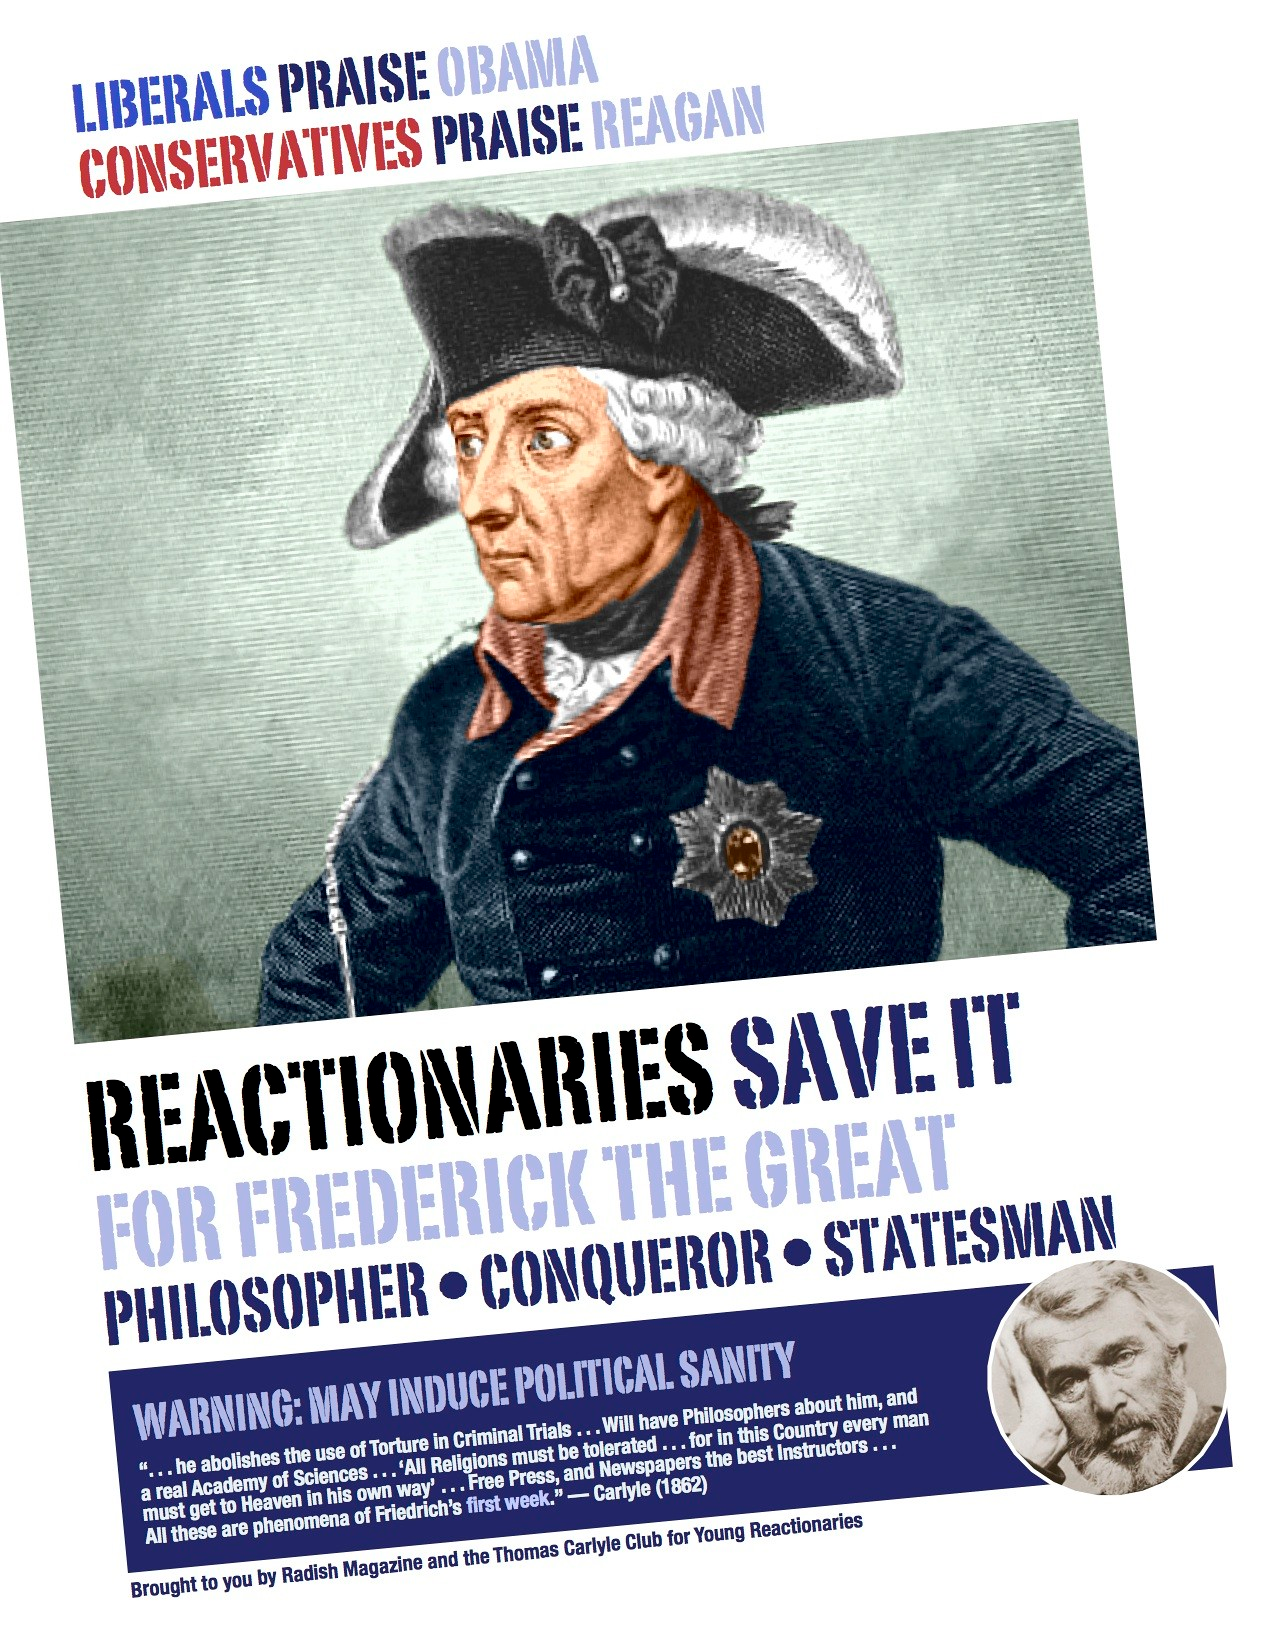
\includegraphics[width=0.7\linewidth]{images/carlyle-neorreactionaries.png}
  \caption{Federico el Grande en un cartel de propaganda neorreaccionaria}
  \label{fig:federico}
\end{figure}

En ella se aprecia el cartel propagandístico en inglés de un sitio web de Estados Unidos de América. Se mira a Federico el Grande con una leyenda que dice que, a diferencia de los liberales, que rezan a Obama, y de los conservadores, que lo hacen para Reagan, la visión neorreaccionaria simpatiza con Federico, rey alemán, filósofo, conquistador y hombre de Estado \autocite{huiUnhappyConsciousnessNeoreactionaries2017}. Los neorreaccionarios son un movimiento primordialmente compuesto por hombres blancos cisgénero en EUA, creen que mientras que la tecnología y el capitalismo han avanzado, la democracia ha obstaculizado el desarrollo económico, que para ellos constituye el \emph{telos} de las sociedades. Proponen un regreso al tradicionalismo en roles de género, jerarquías sociales y a la monarquía \autocite{AskphilosophyWhatNeoreactionarism}. Su posición virilista es la sublimación de resentimientos y de frustración sexual.

Los neorreaccionarios son emprendedores de alta tecnología de Sillicon Valley y su ideología política se proyecta la construcción de una utopía tecnocapitalista. Los neorreaccionarios son hombres resentidos, tristes, que pueden ver los problemas de los que son parte, pero hacen de la crítica un instrumento, y de la soberbia de sus pretensiones heroicas una ideología sobre La Razón. Son hombres enfermos de sospecha, pues todo les es dado a través del arreglo mercantil. Son ciborgs melancólicos, su potencia ha sido castrada por su conciencia de ser el ciudadano ideal, aquel por el que la explotación tiene sentido. No pueden imaginar un futuro afuera de la sociedad mercantil, desean \emph{desear el Estado}. Son el sujeto pleno de derecho, la promesa del Estado moderno. De ahí su frustración, de estar en el tope del privilegio, de su imposibilidad de morir. Su conciencia infeliz y su devenir cínico se manifiesta en su tono irónico. Viven en una tensión entre experiencia y concepto. Para los neorreaccionarios, la Ilustración es un otro alienado del yo, constituye un \emph{pharmakón}, remedio y veneno. El anacronismo y anti-intelectualismo son herramientas de los neorreaccionarios para construir un discurso donde la razón y la ciencia son concebidas para justificar el estado de las cosas. Feminizan los actos de resistencia de activistas para señalar el desvarío de la rabia y descalificar cualquier sublevación como irracional, como terrorismo que atenta contra la sociedad. Para los neorreaccionarios, la voluntad general es como el interés general: la Contradicción hegeliana del yo que se vuelve absoluto, una conciencia triste al saber que Dios ha muerto. De ahí que estos hombres tristes señalen que la \enquote{Catedral} es la iglesia contemporánea de la correctitud política. El síntoma de la conciencia infeliz del neorreaccionario se manifiesta a través de una ironía implacable \autocite{huiUnhappyConsciousnessNeoreactionaries2017}.

\begin{quote}
  \emph{La voluntad general como interés general: la Contradicción hegeliana del yo que se vuelve absoluto, una conciencia triste al saber que Dios ha muerto.}~\autocite{huiUnhappyConsciousnessNeoreactionaries2017}.
\end{quote}

Su apuesta por un regreso al absolutismo ilustrado es el síntoma de un proceso muy curioso en la Historia y de repercusiones políticas importantes. El \emph{meltdown}, concepto apropiado por los reaccionarios que puede traducirse como hundimiento o derretimiento, se refiere a la decadencia del proyecto de Ilustración y es también el título de una obra de Nick Land \autocite{landFangedNoumenaCollected2018}, es también síntoma de una crisis profunda en la civilización moderna que se manifiesta en la ecocatástrofe y el exterminio. Este vuelco a la política monárquica y al autoritarismo son parte de los movimientos de derecha en Estados Unidos cuyas ideas han creado organizaciones que buscan la toma del poder. Que el movimiento neorreaccionario tenga como polos a Donald Trump, empresario septuagenario, y a Pepe la Rana, meme que dio fama a la derecha alternativa \autocite{huiUnhappyConsciousnessNeoreactionaries2017} en el internet estadunidense, muestra dos caras de un mismo malestar en el Estado moderno. La llegada de Trump; el desarrollo altamente personalizado de la industria farmacopornográfica, régimen bio-molecular y semiótico-técnico de producción de subjetividad \autocite{preciadoTestoYonqui2008}; y el auge de foros de adolescentes encerrados en sus sótanos en el sitio web \url{4chan.org}; evidencian que la derecha alternativa se ha apoderado del gobierno del país más poderoso ---y endeudado--- del mundo. Este momento histórico evidencia una era poshistórica, posverdad, caracterizada por el derrumbamiento de la política iluminista de los Estados-nación, basada en la representación estética y racionalidad económica. La complejidad del contexto plantea grandes limitaciones teóricas a la academia de acceder a las raíces del problema.

\begin{figure}[htb]
  \centering
  
\includegraphics[width=0.7\linewidth]{images/pepe.jpg}
  \caption{\emph{Pepe the frog}, personaje de internet famoso por su uso en los memes.}
  \label{fig:pepe}
\end{figure}

La estética reaccionaria parece transgredir las convenciones de \emph{corrección política} necesarias para considerarlo una postura estética. Sin embargo, pese a la ambigüedad de sus postulados, los neorreaccionarios sienten melancolía por una idea de Occidente parecida al despotismo ilustrado que guiaría a la Humanidad al progreso. Para ellos, la cuestión de la productividad y la despolitización tecnocomercial son parte de lo necesario para salvar a Occidente. En el \ref{cha:el-rostro} ahondaré más en la cuestión del derretimiento causado, según este movimiento, por la democracia liberal.

\section{La política \emph{folk} es insuficiente para crear una alternativa}
\label{sec:la-política-folk}

\epigraph{Al enfatizar y permanecer en el ámbito de lo inmediato, la política \emph{folk} carece de las herramientas para transformar el neoliberalismo en otra cosa.}{\emph{Nick Srnićek} en~\autocite{srnicekInventarFuturoPoscapitalismo2017}.}

Tanto los movimientos radicales que están enamorados de la congruencia moral como los liberales, amantes del discurso tecnocientífico capitalista, son el síntoma de una intensa guerra de pensamientos que produce una interioridad psíquica hostil contra sí misma y contra la otredad. La guerra contra nuestro deseo y contra el mundo es un rasgo de lo que Tiqqun nombraría \emph{antropología positiva}, la captura de toda experiencia, de toda técnica, para el Capital. Nuestro deseo no es nuestro. Deseamos al Estado porque su operación principal es hacer que las formas de vida deseen deseo de Estado. En ese sentido es que el Estado moderno, epítome de la modernidad y de las fantasías detrás del concepto de Occidente que profesan los neorreaccionarios, es una religión.

La política folk es un concepto presente en las estrategias de guerra de los neorreaccionarios. Foros de internet de hombres blancos alienados que miran pornografía \emph{gore} dieron forma a los primeros memes del internet. En este contexto, internet se convirtió en una plataforma de debate político cuyos agentes fueron hombres resentidos con un alto capital tecnopolítico, es decir, capital sobre los códigos de tecnología en cadenas de producción y de significación social. Política folk designa a una caricatura política de la izquierda contemporánea como grupos de puritanos de carácter sectario y resentidos contra la sociedad por su incapacidad de pertenecer.

Esta sección trata de bosquejar la política folk con la seriedad que lo hicieron Alex Williams y Nick Srnicek en su texto \emph{Inventar el futuro}. Mi intención aquí es describir el escenario que dio origen al movimiento neorreaccionario. El \emph{\#altwoke Companion} propone el siguiente esquema \autocite{AltWokeCompanion2017}:

\begin{figure}[htb]
  \centering
  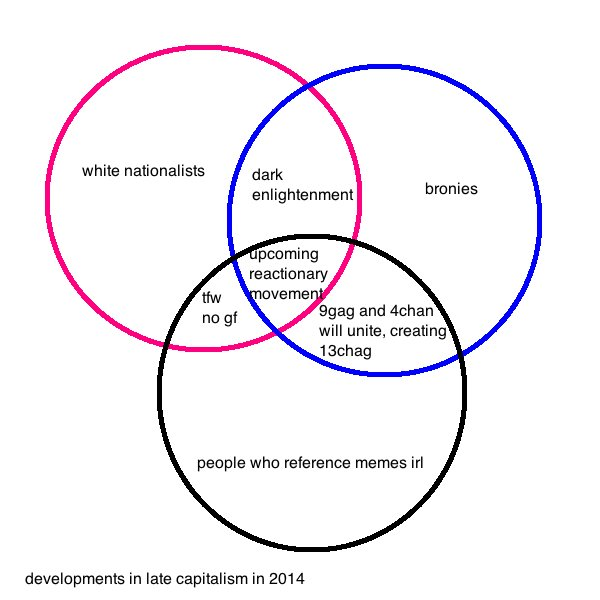
\includegraphics[width=0.7\linewidth]{images/internet-capitalism-2014.png}
  \caption{Desarrollo del capitalismo tardío en 2014, según un foro de internet.}
  \label{fig:capitalism2014}
\end{figure}

Según la derecha alternativa de internet --probablemente los foros más cínicos de estos días-- la izquierda se posiciona como una Catedral dogmática que abraza y reproduce el marxismo cultural posmoderno para planear una guerra, un sabotaje en contra de la civilización occidental. La crítica de los neorreaccionarios al sentimiento religioso-folklórico es que es moralista y es una posición primitivista. La Catedral es el principal centro de resistencia frente a la agenda de productividad del movimiento neorreaccionario. Además de la connotación de dogmatismo religioso, la Catedral también se refiere a la élite progresista de izquierda liberal. Distintos grupos de derecha en internet se dedican a señalar cómo la izquierda se destruye a sí misma a través de la política folk, que identifican con el rechazo a las instituciones y con un activismo micro, local, autocomplaciente.

La Catedral representa la herencia de Occidente y es, por ello, un enemigo del progreso. Los neorreaccionarios toman partido por la utopía tecnocapitalista y consideran a la política como un enemigo para sus fines. La fantasía biónica de Nick Land, cuya posición poshumanista crea una dicotomía entre una superinteligencia antihumanidad y la emancipación universal, yace en el trasfondo de estos proyectos. Singapur y Hong Kong son ejemplos de la utopía pospolítica.

La política folk es una experiencia de la política como droga, como mero entretenimiento, algo que en los foros de internet describen como \emph{choose your own adventure}. Srnicek y Williams la describen como una política afectiva, micro, sin ser efectiva a nivel macro. Ocurre por tres razones:

\begin{itemize}
  \item Incapacidad de lidiar con la complejidad, con el complejo entramado de formas de violencia y de sujeción al poder del capital. Por ejemplo, en los mercados, donde diversos ciclos de producción están relacionados directamente a otras variables y ellas, a su vez, dependen de fenómenos macroeconómicos poco accesibles a la gente común.
  \item Reacción a las instituciones políticas de izquierda tradicionales, a lo que los neorreaccionarios llaman la catedral por un comportamiento sectario centrado en la organización comunitaria. Surge con la decadencia del movimiento hippie y se caracteriza por un vuelco al localismo y horizontalismo \autocite{TyrannyStucturelessness,TyrannyTyranny}. 
  \item Reacción simbólica al espectáculo político. Es decir, frente a la industria de los medios de comunicación, que transforman toda experiencia de vida en representación capitalizable, la política folk decidió evitar cualquier confrontación mediática y de la farándula de la militancia institucionalizada para volcarse al activismo hiper-local que construyera alternativas comunitarias \emph{in-situ}. Esta situación se explica en parte por la disolución de los polos EUA-URSS después de la caída del muro de Berlín.
\end{itemize}

La política folk es un concepto que se refiere a una forma que surge tras la caída de los grandes movimientos hegemónicos y se puede localizar en la época posmoderna como una condición de marginalidad tras la victoria del capital sobre las otras grandes narrativas históricas. Acción directa, democracia real y anti-jerarquía son algunas de las características de esta práctica política. Pareciera que hoy en día sobran tácticas políticas y gestos de desobediencia pero la cuestión sobre cómo crear una alternativa política a escala global o molar sigue abierta y ha sido olvidada por buena parte de la izquierda contemporánea. \emph{Inventar el futuro} aborda esta cuestión con un programa político que denosta la participación folklórica de distintos grupos de izquierda para lanzarse a la exploración de un proyecto económico hegemónico que se lanza a la disputa por el universalismo, el progresismo y otras categorías que forman parte de la herencia de la Ilustración \autocite[p.~14]{srnicekInventarFuturoPoscapitalismo2017}. Si bien es una propuesta coherente al interior del Estado para crear una sociedad poscapitalista, su base sigue dependiendo en la ligadura economía-Estado, por lo que su respuesta al desarrollo voraz del capitalismo sigue siendo occidental. Es decir, presupone que la \emph{forma de vida} por excelencia es la ciudadanía y no atiende realmente a las razones que producen a la economía mercantil como un régimen de deseo.

Pese a que Srnicek y Williams abordan con relativa claridad el fenómeno, no parece ahondar demasiado en la naturaleza psíquica de la sociedad mercantil contemporánea. La política folk es problemática por diversas razones. Una de las más relevantes para este trabajo tiene que ver con cómo lidiar con la complejidad del mundo. Es ahí donde profundizar en la relación entre Estado y economía se vuelve sumamente relevante. La aparente autarquía de los mercados funciona a través de un caótico entramado de transacciones.

La necesidad de coherencia y la invisibilización de los privilegios, lo opuesto a lo que Donna Haraway llamaría \emph{conocimiento situado}, hace que las izquierdas en Estados Unidos caigan en el descrédito mediático a través de falacias argumentativas que hace ver a las personas de izquierda (señaladas en tono irónico como \emph{Social Justice Warriors}) como gente inestable e incoherente en lo que respecta a una agenda política común y popular. En general, los movimientos de izquierda son aplastados mediáticamente a través del cinismo y la ironía. Por esa razón, las estrategias de izquierda tienen que tener en cuenta que lo que caracteriza a las posturas conservadoras, tradicionalistas o reaccionarias, es el \emph{resentimiento}, operado a través de la retórica del cinismo contemporáneo.
 Una alternativa política debe partir del reconocimiento tecnomaterialista y de la estrategia política. En el mismo ensayo, \autocite{huiUnhappyConsciousnessNeoreactionaries2017} señala que la modernidad es más bien la dominación tecnológica que despoja a cualquier forma social de interioridad a través de un proceso de apropiación tecnopolítica. Es decir, la cuestión tecnológica está en el centro del problema político contemporáneo.

La tiranía de la ausencia de estructura es un problema de reconocimiento del deseo. Yo considero que hay algo de cierto en el diagnóstico de las derechas de Estados Unidos con respecto a las dificultades de las izquierdas pero adjudico las causas a un proceso sociológico señalado en \autocite{TyrannyStucturelessness}. Presas de la nostalgia, muchos intelectuales de \emph{ethos} virilista reproducen un dogmatismo y control sectario incluso en los grupos de activistas. Las izquierdas más reconocidas en los medios masivos están compuestas de hombres virilistas de prácticas autocomplacientes que buscan autoridad sobre las demás personas a través del carisma.

\section{La época de la Ilustración es también llamada el siglo de Federico}
\label{sub:la-época-de-ilustración}

\epigraph{\enquote{Igualmente, un sacerdote está obligado a un puesto que fue aceptado bajo esa condición. [\ldots] La Ilustración es la potencia o condición histórica de discernimiento propio en materia de religión}}{\emph{Immanuel Kant} en~\autocite[p.~96]{kantQueEsIlustracion2009}}

La propuesta de Kant le hablaba a los príncipes alemanes como agentes de la Historia universal, pero se volvieron cínicos. La causa es que la crítica en el seno del Estado moderno encarna una contradicción manifiesta en el teatro político de la \emph{publicidad}. Este proceso tiene un equivalente mediático, el periódico. Podemos identificar la religiosidad del proyecto de Estado en la máxima kantiana de la fe en la acción pública. Su pregunta es cómo plantear la fe a través de la acción crítica como la finalidad de la Historia, y en consecuencia, como objeto del Estado. Su respuesta es tan satisfactoria que permite el despliegue y sofisticación de las cortesías y los manuales de etiqueta que caracterizaban a la política monárquica y al teatro de las cortes y los parlamentos europeos.

Paradójicamente, la democracia liberal tiene su génesis en esos procesos y reproduce la lógica de la ciudadanía griega de la pertenencia a la polis, de la capacidad de participar de los asuntos públicos periódicamente.

Federico fue el primer soberano de la pluralidad ética como solución a la guerra de religiones. Acogió a Voltaire y señaló que la tarea del Estado era llevar la ilustración y la cultura hasta el último rincón del mundo. Es decir, se trata de la puesta en operación de un dispositivo de guerra. En la modernidad, la superación y captura tecnológica se convierten en la forma de apropiación del Estado de toda forma de interioridad.

El progreso y el universalismo son conceptos en disputa. Los sentidos de la Ilustración según el artículo de Hui son, por un lado, el de Diderot y por otro el de Hume. Algo parecido a la tensión entre el espíritu estoico y el escéptico de los que habla Hegel. El progreso ha sido malentendido. La modernización se convirtió en una empresa colonial y de esclavitud.

En su \emph{Filosofía de la historia}, Kant plantea una fe para el progreso basada casi en su totalidad en la acción. El filósofo alemán escribió desde un principio para los príncipes que pudieran leerlo con la intención de suscitar en ellos el interés por dar un curso racional e iluminista a la historia a partir de la razón. Su fe en la Historia es también un llamado a la acción para los príncipes. Pero la publicidad de la que habla Kant produce un simulacro. Reproduce la lógica de las cortes como el manual de comportamiento de la vida pública y neutraliza toda forma de violencia, todo conflicto confesional, en un debate cuya plataforma técnica es la escritura y su medio la prensa escrita. En este sentido, la prensa es una consecuencia de la imprenta vernácula y la reafirmación de la escritura como plataforma general de la teoría y de la práctica. El texto se vuelve la unidad de información que permitirá la transición de sociedades soberanas a sociedades disciplinarias.

\epigraph{La operación principal del Estado consiste en transformar todo deseo en deseo de Estado.}{\emph{Gilles Deleuze} en~\autocite{deleuzeMilMesetasCapitalismo2002}.}

El hecho de que la derecha alternativa plantee una posición neomonarquista basada en ideas protofascistas atañe a un proceso histórico nacido en tiempos de la posguerra y es lo que Agamben señala como el estado de excepción, donde el exterminio es la normalidad. La finalidad de los neorreaccionarios es reinstaurar la vieja gloria de la civilización occidental rompiendo con la inercia integradora del proyecto imperial y abogando por una separación entre semejantes ilustrados frente al mundo salvaje. La ironía de estos sujetos expone los arreglos epistémicos de la sociedad poshistórica (y por extensión, posverdad) y expone los defectos de la Ilustración. La cuestión de fondo tiene que ver con la forma como el Estado ha configurado todas las subjetividades y en cómo se instaura a través de la necesidad, transmutando todo deseo en interés. De este modo, el interés es el elemento fundacional de la \emph{societas}. Y el público no es otra cosa que los propietarios argumentando en favor de su posición en el arreglo mercantil.

Para la disputa de los sentidos de la Ilustración, hay que entender para qué opera en realidad el Estado moderno y cómo se vale del discurso de la Ilustración y de la Ciencia para justificar su poder, para crear una religión de sí mismo. Como actitud de fondo al drama contemporáneo, el cinismo surge como instrumentalización de la razón a partir de la distinción entre razón pública y privada. Basta recordar que Kant fue un gran admirador de Federico el Grande, que decía sin reparo \enquote{críticad cuando queráis pero obedeced}. El cinismo consiste en la victoria de la tristeza y de la melancolía. La toma de partido del cínico es una respuesta a la contradicción al preferir la servidumbre de sí mismo a la libertad a partir del reconocimiento del deseo afuera del deseo de Estado.

\section{El neoliberalismo se ha apropiado del futuro}
\label{sec:el-neoliberalismo-se-ha-apropiado-del-futuro}

¿Cómo recuperamos la imaginación política? Mientras que Francis Fukuyama plantea el fin de la guerra de ideas \autocite{fukuyamaFinHistoriaUltimo1992}, Samuel Huntington plantea el choque de civilizaciones tras la victoria de la democracia liberal \autocite{huntingtonClashCivilizationsRemaking1996}. Es entonces cuando comienza la guerra contra el terrorismo y la transición de la posmodernidad a la era digital. Tenemos como ejemplos el \emph{Global Action Day} o el movimiento Antiglobalización como reacciones al proyecto neoliberal. Sin embargo, vivimos en un tiempo donde los mecanismos de poder se vuelven difusos y, en el peor de los casos, \emph{capturables}. Podríamos decir que es el fin del maniqueísmo, pues la ruptura de amenazas exteriores y el vuelco a la política interior y a externalidades de globalización como prioridad de seguridad de los gobiernos mundiales, actúan a través de múltiples registros. En ese sentido, si los Estados-nación veían su política a la \emph{Westfalia}, hoy nos enfrentamos a entidades transnacionales que hacen su propia legislación. En pocas palabras, se trata de otro repliegue del imperio, donde la aceleración de las contradicciones llega hasta un nuevo punto de exterminio: la automatización y, en medio de ello, lo probable de la singularidad \autocite{fraseFourFutures2011,fraseFourFuturesVisions2016}.

La lógica de medios y de instituciones nos condicionan al consumo. Hay que tomar posición sobre el mercado. Durante mi investigación me encontré con la dificultad conceptual de relacionar y ser capaz de diferenciar los conceptos de Estado, mercado y capitalismo. Quería entender cómo se produjeron los discursos que hacen que distintos componentes histórico-políticos dieran forma al estado actual de las cosas. Aprendí que en el neoliberalismo, la ciencia se transforma en el discurso justificador y la sociedad se adapta para ejercer un control más exquisito y perfecto sobre el deseo. Experimentamos aquí una transfiguración del Biopoder en despliegues cibernéticos que desmaterializan los dispositivos de poder, traduciendo las normas en impulsos eléctricos y bioquímicos y reduciendo al capitalismo, cada vez más, al mero flujo y tráfico de información. Este proceso evidencia al Principio, como máscara del Imperio, para desplegar un régimen de normas y dispositivos, para despersonalizar todo poder y para conducirnos a la agonía misma del Estado en el fin de la historia. 1989 es un símbolo de ese proceso. La caída del muro de Berlín anuncia el fin de la historia y el auge devastador de la hegemonía neoliberal revela al Imperio como el aparato patético que tiende a controlar cualquier posible eventualidad.

Muchos hombres activistas de izquierda niegan comportamientos machistas y totalitarios en los movimientos en los que operan. Sin embargo, el conocido artículo \emph{Tyranny of Structurelesness} desarrolla los modos informales de control de las autoridades de facto en las organizaciones y señala el comportamiento virilista como un problema de importancia considerable. Una de las múltiples réplicas a este ensayo, \emph{Tyranny of Tyranny} profundiza en lo costoso del cinismo de aquellos hombres aburridos que Tiqqun denominaría como bloomescos \autocite{TyrannyTyranny}. Su comportamiento reproduce el deseo de Estado a través de la deuda, creando una suerte de impuesto moral por el que las personas activistas se redimen, sin buscar necesariamente acciones estratégicas, como si se tratase de una guerra.

Srnicek y Williams apuntan a la construcción de imaginarios que permitan lidiar con la complejidad del mundo contemporáneo para navegar en un terreno político donde el discurso tecnocientífico y la retórica están al servicio de pensamientos que podríamos agrupar en la categoría de derecha alternativa pero también de nuevas derechas. Cómo crear una masa crítica revolucionaria con poder suficiente como para dar un salto más allá de la cultura de la crisis, del Espectáculo de la catástrofe. Antes de continuar, debemos advertir nuevamente sobre la capacidad del Estado de asimilar otras expresiones y voces, capacidad nos deja sin ninguna posibilidad legítima de hacer frente a él. Ni las protestas interminables ni el terrorismo total ni la socialdemocracia reformista son ahora dignas de considerarse estrategias políticas. La práctica política del futuro es tan difusa como los dispositivos con los que está (des)armándose a cada momento.

Para recuperar la imaginación política hay que entender cómo se produce la imagen en el posfordismo, con la cibernética aumentando la dependencia del humano a la máquina.

Si bien el proceso constituyente por el que abogan propuestas como el populismo de Laclau y Mouffe \autocite{laclauRazonPopulista2016} o la posición de Hardt y Negri \autocite{hardtImperio2005} es clave para la revolución, el elemento transformador (por radical y revolucionario) se encuentra en realidad en el poder destituyente, que es la forma en que se generan resistencias escalables tan efectivas que puedan suplir al capitalismo (y en consecuencia, hacer cada vez menos necesario al Estado). El horizonte ético de este poder destituyente ha sido señalado por Hardt y Negri en Imperio y por el Comité Invisible, en las reflexiones sobre la revolución \autocite{comiteinvisibleAhora2017}. Este consiste, entre otras cosas, en retomar la lucha spinoziana por cultivar potencias para el libre juego de las formas de vida. Claro está que los problemas económicos que habrá que enfrentar para hablar sobre el fin del capitalismo son vastos y complejos, pero para abordarlos haremos una breve disección en los componentes de este modo necropolítico de producción para analizar particularmente los conceptos de mercado, eficiencia y efectividad.

Los zapatistas creen que su planteamiento es más moral porque reivindica la lucha de los de abajo y en ese sentido reafirman al capitalismo como poder dominante y no le pueden quitar el componente simbólico de dominación porque lo reconocen. además, al asumir su papel no se comprometen con hacer del zapatismo un modo de vida para todas las personas porque no ofrecen alternativas reformistas que acerquen a la gente, como el blockchain o la organización descentralizada. Y si lo hacen, no es visible.

En \emph{Four Futures}, Peter Frase propone cuatro escenarios para simplificar las posibilidades políticas que hay para las próximas décadas. A este análisis vale la pena sumar otra cuestión: dentro de las principales estrategias del Estado se encuentran la guerra contra el terrorismo y un régimen económico que, en referencia a Preciado, llamaremos farmacopornista \autocite{preciadoTestoYonqui2008,fraseFourFuturesVisions2016}.

\section{El problema político \emph{real} es la captura tecnológica del deseo}
\label{sec:el-problema-político-real}

\epigraph{(\textsf{Pregunta}) ¿Si pudiera ver un documental sobre un filósofo, sobre Heidegger, Kant o Hegel, qué es lo que querría ver?\\ (\textsf{Respuesta de Derrida}) Que hablen de su vida sexual. ¿Quería una respuesta rápida, no? Su vida sexual.}{\emph{Jacques Derrida} en~\autocite{dickScreenplayEssaysFilm2005}.}

El problema de la Historia de Hegel es su posición idealista y lo que ella dice de la guerra de religiones. La victoria de la forma Estado capitalista es también la tensión entre protestantismo y catolicismo, entre la representación y la iconografía. Sin embargo, además de moverse por el deseo de \emph{ser como}, de encarnar la figura de Cristo, de reproducir la lógica de la representación, las formas de vida actúan pulsionarmente, en un dominio psíquico que, pese a los grandes esfuerzos del Biopoder, permanece oculto, sin que por ello sea no explotable. Somos máquinas deseantes, formas de vida. La explicación de la neorreacción tiene una instancia molar, la de la gran narrativa del Estado, la de un lenguaje para sí que configura lo real en el tiempo y en el ambiente. Sin embargo, hay otra posible explicación a otra nivel molecular, psíquico, que atañe a la respuesta de las formas de vida a los estímulos. Bajo esta explicación, los neorreaccionarios son sujetos frustrados y castrados sexualmente. Configuran la multitud que toma partido por el resentimiento sexual y por una pulsión ---retomando a Preciado--- \emph{snuff}.

El tecnomaterialismo se parece mucho a lo que imagino como cruce entre una forma molar y otra molecular de analizar el poder. En relación con la escasez de recursos, el deterioro y acelerada pauperización son reales. Frente al tecnofascismo se necesita abrir otra vez la cuestión del Partido y eso solo se puede lograr analizando dónde se sitúan los deseos. Mientras que Nick Srnicek y Alex Williams buscan la configuración de un movimiento político de vanguardia, Preciado, retoma el análisis crítico sobre las condiciones tecnopolíticas de dominación y propone una visión del trabajo desde el concepto de \emph{potentia gaudendi} o fuerza orgásmica para entender otras formas de producción de valor en el mercado. Desarrollaré el argumento de que hay una tensión entre la economía como el problema mismo y la economía como condición emancipatoria de la propia economía. Me interesa entender cuáles son los límites tácticos y horizontes que, a partir del mercado, puedan contribuir a una práctica difusa de la política radical, tendiendo siempre como horizonte la potencia común para el libre juego de las formas de vida.

La crisis tiene dos caras: por un lado, la ecocatástrofe producida por el despliegue trasnacional del capital, y por el otro, el cinismo y el nihilismo como síntomas de la crisis de la religión de Estado (o lo que Fukuyama llamaría \enquote{fin de la historia}). No deja de ser claro que, a pesar de lo anterior, la lucha inicia destituyendo el Espectáculo, pero se gana en el terreno de los recursos económicos, por la dificultad de obtener y gestionar bienes y necesidades. Tecnomaterialismo considera los procesos productivos como lo que configura las relaciones sociales. Desde este punto de vista, somos configuradas por las interfaces y el ecosistema que nos produce. El problema de la falsa conciencia ilustrada quizá tiene que ver con una respuesta psíquica colectiva que produce amos y esclavos a través de los flujos de codificación del deseo.

Crítica al optimismo tecnológico: El sueño utópico de marxismos y anarquismos, de un mundo donde la tecnología supondría la emancipación del hombre, es técnicamente posible. Es decir, en la actualidad existen suficientes herramientas no solo para aliviar la pobreza sino para garantizar la libertad efectiva, sintética de acuerdo con Nick Srnicek, para todas las personas en el planeta. Sin embargo, el presente es también el momento de la instauración definitiva de la crisis y de la invisible aceleración de la ecocatástrofe, que silencia las voces de quienes no tienen rostro y las confunde con el ruido transparente de los circuitos de producción de sentido del Imperio. Las consecuencias del fin de la historia no han sido otras que la reafirmación y reconfiguración de la autoridad estatal en dispositivos de poder cada vez más difusos. El síntoma más claro de la crisis está en la crisis de la democracia liberal, que resulta cada vez más rebasada frente a las distintas subjetividades y a la cuestión tecnológica ---que está directamente relacionada con el trabajo.

Todo pensamiento es estratégico en la medida en que el problema político contemporáneo es el entramado de tecnologías que producen los dispositivos de la cibernética. Thiels, uno de los inversionistas ángel más aclamados de Sillicon Valley, es una muestra de esto. Parte de una experiencia, de un \emph{pathos}, parecido al de Spengler. En la visión de este teórico podemos encontrar una experiencia muy semejante a lo que Tiqqun describe como el Bloom. La Ilustración oscura\footnote{Traducción nuestra para referirnos al concepto de Dark Enlightenment de Nick Land, del que parten los neorreaccionarios para fundamentar sus posturas. \autocite{DarkEnlightenmentNick2012} parte de una oposición entre libertad y democracia \autocite[p.~5]{huiUnhappyConsciousnessNeoreactionaries2017}}. Lo que se oculta detrás de su posición es una vaguedad conceptual en la que se considera como democracia a la simulación representativa electoral que da forma a la mayoría de los Estados-nación contemporáneos.

El resentimiento es el sentimiento principal de los neorreaccionarios. ¿Por qué es preocupante este resentimiento? Simplemente porque este sentir contagia a formas de vida que acumula agencia tecnomaterial. Es decir, capacidad para transformar la realidad. Lo que significa que de los cuatro escenarios posibles para un futuro cercano, este grupo probablemente decida de hecho hacia qué camino transitan las sociedades en su conjunto.

En la actualidad, el descontento por la \enquote{democracia liberal} es parte de una disputa más profunda sobre el progreso, la democracia y el universalismo. La corriente neorreaccionaria es una de las más férreas opositoras a la democracia liberal y es quizá aquí donde tengan un punto de comunión con diversas posiciones políticas que también se le oponen. Sin embargo, es necesario recordar que la alternativa para los neorreaccionarios no es otra sino una utopía tecnototalitaria ciudadanista.

\begin{table}[htb]
  \caption{Escenarios planteados en \emph{Four Futures} respecto al porvenir global.}
  \label{tab:ubicua}
  \centering

  \begin{tabular}{ccc}
    \toprule
    & \textbf{Abundancia} & \textbf{Escasez}\\
    \midrule
    \textbf{Igualdad} & Comunismo & Socialismo\\
    \textbf{Jerarquía} & Rentismo & Exterminismo\\
    \bottomrule
  \end{tabular}
\end{table}

El problema político es un imaginario del futuro que nos lleve al escenario ideal en \emph{Four Futures} El problema de acción es la tiranía de la ausencia de estructura. En realidad este fenómeno se da porque es realmente complicado hacer una alternativa que ataque diferentes violencias transversalmente. La falta de estructura se explica como un arreglo económico sobre el deseo donde prevalece la mala conciencia, el resentimiento y latencias de un orden jerarquizado y estamentario (unión con precariedad-jerarquía de \emph{Four Futures}.

Una de las cuestiones que más ocupa a Fraser es la cuestión de cómo podría darse un escenario de comunismo real si las clases de personas ricas y propietarias opondrán resistencia de forma violenta a cualquier insurrección. Para Tiqqun, la guerra civil es el libre juego de las formas de vida, el principio de su coexistencia. Las sociedades tradicionales conocían el robo, la blasfemia, el parricidio, el rapto, el sacrificio, la afrenta y la venganza. Por otro lado, las sociedades modernas se apropian de la capacidad de decidir sobre cualquier conflicto social. La violencia es aquello de lo que hemos sido desposeídos, y aquello de lo que hace falta ahora reapropiarse.

El Estado es una religión que captura nuestro deseo y lo incorpora al contrato social. Un movimiento real debe permitir a las personas ser agentes de su deseo. Por eso la ciudadanía no resuelve nada, es deseo de deseo de Estado. En el deseo de Estado manifiesto religiosamente a través del trabajo, perviven latencias de sociedades premodernas adaptadas a un mito que adapta las jerarquías tradicionales y la obediencia al desarrollo de las formas de producción de valor de las mercancías. La religión de Estado transforma deseo en interés. el cinismo es el dispositivo discursivo que produce placer a quien se congratula de su impotencia, de instrumentalizar la crítica.

Históricamente, la gestación del Estado moderno se sitúa en la guerra de religiones como contexto histórico de la guerra civil en la sociedad tradicional y recuerda un poco a la reflexión de Hegel sobre el judaísmo y el cristianismo en la Historia de la conciencia absoluta. La impronta ética de las visiones afuera del Estado moderno hoy en día, no son capaces de plantear una totalidad plena de sentido, un sentimiento de universalidad. Mientras, la neorreaccion hoy en día consiste en la construcción de intenciones racionalistas y bajo el discurso tecnocientífico, de una utopía tecnocapitalista cuyos exponentes máximos son Hong Kong y Singapur. Para mí, este fenómeno muestra dos caras de un profundo proceso de alienación que tiene que ver con la correcta asimilación parasitaria del capitalismo al Estado moderno. En el siguiente capítulo analizaremos al Estado operar como entidad tecnológica tanto en un sentido tecnomaterial como en uno libidinal a través de la religión.
\chapter{El Estado moderno no es otra cosa que la religión de Estado}
\label{cha:el-estado-moderno}

El Estado moderno nace para poner fin a la guerra de religiones. Tiene un cuerpo que captura y que produce. Se vale de una neutralidad central para poner fin a la guerra de religiones y es condición de garantía para la pluralidad ética, para la coexistencia de las religiones si se supeditan a la concepción capitalista del trabajo. En ese sentido, el Estado supera todas las formas anteriores de religión. \emph{La religión de Estado} captura el deseo a través de la economía. De acuerdo con Tiqqun, el fin de la guerra de religiones está en la conversión y no en la asunción de las formas de vida. La hostilidad propia de la guerra de religiones se transfiere a una hostilidad general hacia el otro en su forma de ciudadano.

En ese sentido, el súbdito y el soberano son dos caras del mismo proceso de estamentación. La apropiación del deseo tiene como objeto producir el interés de reproducir un rol en la jerarquía y suprimir o dar cauce a cualquier pulsión. Ambos viven para contener a cada \emph{forma de vida} en su Yo incorporando representaciones del propio cuerpo y de la psique. Estos sujetos son los agentes del aparato de captura y se encargan de darle sentido al trabajo y a la producción para que su finalidad sea siempre el plusvalor, la utilidad. La curialización de los guerreros en las cortes es buen ejemplo \autocite{tiqqunIntroduccionGuerraCivil2008}. Eso pasa con la militancia en los tiempos de la política folk, cargada de manuales de etiqueta y simbolismos sin demasiado alcance tecnomaterial (votos, recursos, influencia o base social).

Retomando la introducción, el neorreaccionario aboga por el despotismo ilustrado. Esta señal es muestra de la configuración imperial del Estado moderno contemporáneo, que es a su vez, su crisis. A continuación doy una perspectiva a partir de \emph{Tiqqun} sobre cómo ha ocurrido este proceso y a qué responde la existencia histórica y la crisis del Estado moderno cuyo fin ha sido poner fin a la guerra de religiones. Para el Comité Invisible, la Historia del Estado moderno comienza como una posición frente a la guerra de religiones y la época contemporánea se caracteriza por una crisis profunda de la religión de Estado. A lo largo de este capítulo haré un bosquejo del concepto del Estado sin más a partir de su funcionamiento a través de máquinas y aparatos. Lo anterior me servirá para explicar por qué el Estado moderno no es otra cosa sino la religión de Estado y cuáles son las repercusiones de este proceso a nivel molecular. Es decir, cómo el Estado afecta a las formas de vida y cómo el Estado se erige como el principal productor de subjetividad llevando la guerra a la vida interior de cada \emph{forma de vida} para que en el dominio público prevalezca la neutralidad.

En este capítulo~\ref{cha:el-estado-moderno} desarrollaremos la cuestión de los aparatos y agentes del Estado que fungen como su aparato de captura del deseo.

\section{El Estado se vale de una máquina de guerra capitalista y su propio aparato de captura}
\label{sec:el-estado-se-vale-de}

Comenzaré con explorar el concepto de Estado sin más. De acuerdo con Deleuze y Guattari, en un sentido noológico, el Estado es \emph{Urstaat}, es el \enquote{Logos}, \enquote{La Palabra}, un espacio estriado en cuya configuración se crea la correspondencia cosa-palabra. Es decir, el mundo es un todo fragmentado por el Estado, por la palabra, por la correspondencia unívoca que hay entre cosas, enunciaciones y acciones \autocite{deleuzeMilMesetasCapitalismo2002}. Lo opuesto al Estado sería un espacio liso, donde el lenguaje se resbala de las cosas y el nexo cosa-palabra es más casual. En una metáfora, el Estado produce círculos ideales en oposición a un redondel, que es una forma circular imperfecta, concreta. Asume como real aquello configurado a través del lenguaje y no a través de la materialidad, de lo corporal, de su conformación técnica. En un sentido ontológico, las esencias difusas, aquellas que no produce el Estado, son continuas, extraen de las cosas una determinación que más que la coseidad, es la de \enquote{corporeidad}, implica un espíritu de cuerpo. Para desarrollar este argumento, los autores explican que si los orígenes del número se remontan a la cifra, a la necesidad de contar, el Estado plantea un número numerante, que da al número la correspondencia cosa-palabra. Busca regir ahí para dar al pensamiento una forma de interioridad, una realidad intrínseca, y darle a esta interioridad una forma de universalidad: \enquote{la finalidad de la organización mundial es la satisfacción de los individuos razonables dentro de los Estados particulares libres}. De ese modo, el fin del Estado es convertir al pensamiento en máquina de guerra, ponerlo en relación inmediata con el afuera. Es \emph{imperium} y república al mismo tiempo \autocite[pp.~380, 381, 397]{deleuzeMilMesetasCapitalismo2002}.

Para entender lo anterior me resulta muy útil el concepto de agenciamiento, que es la correspondencia cosa-palabra, donde la significación procede de agentes colectivos y de un conjunto de enunciados que disponen a los cuerpos. El agenciamiento o la instancia concreta del Estado es siempre histórica, compuesta por agentes que significan los hechos históricos y las relaciones entre objetos para ciertos fines. El Estado moderno como manifestación del \emph{Urstaat}, cuya etimología \emph{st} significa lo estático, se vale de dos medios principales para sus operaciones sobre la subjetividad y sobre las instituciones: la policía y la publicidad. El fin de estos medios es transformar toda \emph{forma de vida} en ciudadanía, en deuda al E\emph{st}ado. Antes de desarrollar los medios del Estado moderno, señalaré algunas cuestiones sobre el funcionamiento del Estado sin más.

El Estado opera a través de una ciencia de las velocidades o dromología, una forma de saber que analiza el poder desde sus operaciones técnicas y desde sus velocidades. Más allá de las posiciones contractualistas, el Estado sin más, como categoría ontológica, dispone a la interioridad subjetiva al afuera, a la vida psíquica de las formas de vida al ritmo de una máquina de guerra social que permite al Estado expandirse como una categoría del pensamiento. Este sentimiento de totalidad es descrito por el Comité Invisible en la Introducción a la guerra civil como una neutralidad central, como la idea de lo uno, como una configuración estriada del espacio. De esta manera, el Estado configura una forma total de lo \emph{real}, con tiempos, velocidades y disposiciones de objetos a fines explícitos y sobre todo, diseñados para la guerra. La forma en que el Estado construye sus herramientas es siempre como armas destinadas a la captura. Es la ruta ingenieril, una posición técnica \autocite{comiteinvisibleNuestrosAmigos2015}. El Estado domina a través del arte militar, de la guerra. Entre sus tácticas, estría, es decir, fragmenta, el espacio sobre el que reina o usa espacios lisos para la comunicación de espacio estriado. Es decir, se apropia de los flujos y continuidades para reproducir una lógica estriada del mundo \autocite{deleuzeMilMesetasCapitalismo2002}. La dromología de Paul Virilo señala que en ese sentido, el poder político del Estado es \enquote{polis}, policía, red de comunicación. Ve al Estado como \emph{échangeur routier} (ingeniero) y a la dromología como el sistema proyector y proyectil. La velocidad es la cuestión central al analizar las cualidades técnicas de armas y herramientas. De ahí que el nacimiento de los Estados-nación requirió de la captura y de la puesta en marcha de una economía de guerra donde las agrupaciones de mercenarios nómadas se convirtieron en ejércitos al servicio de un soberano. Esto nos muestra la capacidad del Estado de producir redes de comunicación que son en sí la arquitectura del control, de la apropiación de los caminos para el cobro de una renta que sostiene los flujos económicos del Capital.

En un sentido sociohistórico, El Estado se explica más por la progresión de fuerzas económicas y políticas que como resultado de una guerra con frentes y motivos definidos, como algo determinado por la contingencia que produce una narrativa de correspondencia palabra-cosa-Historia. Parece que esta ficción nos muestra que hay una relación de interior y exterior como alcances de la ley del Estado, pues interioridad y exterioridad, máquinas y aparatos, están en coexistencia y competencia, interactúan. Cuando Marx habla del ejército de reserva, no solo se refiere a aquellos trabajadores que ya forman parte del proletariado sino a todos aquellos con una potencia capturable. En ese sentido, el Estado, al tener como fin capturar y explotar las potencias de las formas de vida y orientarlas a un arreglo productivo, transforma todo trabajo de subsistencia --un entendimiento instrumental del trabajo como herramienta-- a trabajo bélico, deuda, trabajo hacia un afuera. Dispone las técnicas del trabajo como arma, como apropiación de la potencia vital para una velocidad de aceleración que tiene como fin la posibilidad de la guerra. Lo que caracteriza al Estado moderno capitalista es que la posibilidad de la guerra está todo el tiempo destinada al aniquilamiento, a la hostilidad absoluta \autocite{tiqqunIntroduccionGuerraCivil2008}.

El Estado pone fin a la guerra de religiones a través de un uso estratégico de armas y herramientas orientadas al capitalismo, a la extracción de valor. El Estado moderno es una máquina de guerra capitalista. Retomando a Marx, el modo de producción asiático es una máquina de guerra despótica. El proyecto de la modernidad consiste justamente en la \emph{transfiguración de la máquina de guerra nomádica en la guerra como la finalidad de toda forma maquínica}. De ahí el papel que tiene la ingeniería y el giro de la economía mercantilista a la financiera. El pragmatismo fue lo necesario para que el Estado protestante se expandiera al incorporar el parásito capitalista y se trata de cierta forma de hacer las cosas que es capaz de hacerse más operativa a sí misma.

En lo que respecta a la máquina social que produce subjetividades, la operación de apropiación se constituye en buena medida gracias a la neutralización de la guerra y a la curialización del guerrero. El nacimiento y profesionalización de los ejércitos nacionales rompe con la lógica de negociación de hordas de bárbaros que ven a la guerra como una cuestión suplementaria. La disciplinarización de la guerra significa una alienación de las formas de violencia, rompe con la posibilidad del conflicto entre pares y de la preparación ritual para la disputa corporal. El desarrollo militar se manifiesta en la célebre frase de Keynes cuando dice que su teoría solo puede probarse en tiempos de guerra \autocite{renshawWasThereKeynesian2016}. A partir del papel tan significativo que tuvo la guerra durante el siglo pasado, durante mi investigación encontré muchas teorías que explicaban la formación del Estado desde posiciones historicistas, colonialistas e incluso descolonialistas. Sin embargo, lo que yo buscaba era una forma de entender la cuestión que me permitiera analizar al Estado desde los procesos que lo configuran, con la intención de analizar sus movimientos como los miraría un ingeniero. Desde ese punto de vista orientado a la acción crítica es que me cuestioné cuáles son los circuitos económicos del Estado moderno.

A continuación presento algunas definiciones de utilidad para analizar las operaciones del Estado moderno como forma histórica total. Para hacerlo, me he valido de dificultosas lecturas de \emph{Capitalismo y esquizofrenia}, particularmente de los apartados \enquote{1227 - Tratado de nomadología: la máquina de guerra} y \enquote{7000 a.J.C. - Aparato de captura}, del artículo \emph{La máquina social} de Carlos Rojas Osorio \autocite{GILLESDELEUZEMAQUINA} así como de una posición aceleracionista de izquierda desarrollada en la revista \emph{tripleampersand} del \emph{The New Center for Research \& Practice} en la ciudad de Nueva York, conocida como \#altwoke \autocite{AltWokeCompanion2017}. En el siguiente apartado desarrollo el modelo de máquina de guerra capitalista y del aparato de captura del Estado. Parto de la siguiente premisa:

\subsection{Bajo el capitalismo, la máquina de guerra capitalista produce mientras el aparato de captura del Estado sustrae}
\label{sub:bajo-el-capitalismo-la-máquina-de-guerra-capitalista}

En este apartado expondré algunas cuestiones relativas a las máquinas. Deleuze y Guattari cambian radicalmente el concepto de deseo que había sido mantenido casi siempre ---con excepción de Spinoza y Nietzsche--- como simple carencia de algo. Por el contrario, el deseo es producción, voluntad de poder; afecto activo diría Spinoza. El deseo como carencia es un concepto idealista, en realidad de raigambre platónica. Deleuze, en cambio, logró ver que el deseo produce realidad.

En la máquina deseante ven Deleuze y Guattari ante todo flujos. Toman la idea de Lawrence: la sexualidad es flujo. Todo deseo es flujo y corte. Flujo de esperma, de orines, de leche, etc. Freud descubrió este flujo de deseo. Ricardo y Marx descubrieron el flujo de producción, el flujo de dinero, el flujo de mercancías; todo ello como esencia de la economía capitalista. Lo que caracteriza al sistema es la apropiación del producto por parte del capital. También Lutero descubrió la religión como fenómeno estrictamente privado, muy acorde con la nueva economía del capital. La producción de deseos es inconsciente, como bien vio Freud. Pero en lugar de la producción de deseos Freud instauró un teatro burgués, porque instauró en el inconsciente la mera representación. En cambio, el deseo tiene poder para engendrar su objeto. Las necesidades derivan del deseo, y no al revés. Desear es producir, y producir realidad. El deseo como potencia productiva de la vida. Por eso Deleuze y Guattari ubican el interés de clase en el inconsciente. Y entre ambos entablan relaciones diferenciales. Por ejemplo, un revolucionario puede serlo al nivel de clase, del interés de clase y, sin embargo, estar dentro de una estructura autoritaria desde el punto de vista libidinal. Viceversa, un revolucionario de la máquina deseante podría ser ajeno a la revolución de la máquina social. Para Deleuze lo decisivo es que el eslabón más débil, el momento de verdadera ruptura llega por el lado de la máquina deseante. Desde luego, no son las condiciones sociales efectivas. Es como la libertad y el determinismo de Kant. Hay un determinismo social, las condiciones objetivas de la máquina social; pero hay también el momento discontinuo de la producción y el deseo. Y es éste, apoyado en las condiciones objetivas, lo que posibilita el acto de libertad supremo que es la producción del deseo. El campo social se carga de una producción represiva o bien de un deseo revolucionario. Este último lo denominan nuestros autores el individuo esquizo. Y el tipo de análisis psicológico lo llaman esquizoanálisis. Sea en la producción represiva que en el esquizo la máquina social es la misma. El esquizo es el productor universal. El sujeto es también producción. Los autores califican a su psicología de materialista: introducir el deseo en el mecanismo social, pero también introducir la producción en el deseo. El esquizo no cree en el yo. La teoría de Freud depende demasiado del yo.

Frente a esta posibilidad de libertad, la economía capitalista organiza la necesidad, la escasez, la carencia. El objeto depende de un sistema de producción que es exterior al deseo. El campo social está atravesado por el deseo. La máquina social es también producción deseante. \enquote{Sólo hay deseo y lo social, nada más}. Paranoia y esquizofrenia son los dos polos de la máquina social. El paranoico tiende a Edipo, a la ley, al orden, al código, al significante. Se proyecta imponiendo el orden, arraigando la autoridad, tiranizando. En cambio, el esquizo constituye la línea de fuga de la máquina social. Busca la producción de la máquina deseante. Nada hay más revolucionario para la máquina social que la máquina deseante. El deseo es primero y fundamental; tiende también a decodificar las estructuras sociales y no coincide con la decodificación que lleva a cabo el capital. Freud se fijó en la represión, pero no logró relacionarla con la represión general que se lleva a cabo siempre en la máquina social. Fue Reich quien asoció correctamente la represión general con cada una de las máquinas deseantes. Por medio de la familia la estructura autoritaria de la sociedad se prolonga hasta sus más íntimos engranajes. El problema de la política lo planteó Spinoza: ¿por qué combaten los seres humanos por mantenerse en la servidumbre como si fuera su salvación? Lo que sorprende es que los explotados no se rebelen o que los hambrientos no roben\autocite{deleuzeMilMesetasCapitalismo2002}.

Deleuze y Guattari hablan de tres tipos de máquina social: la máquina salvaje, la máquina bárbara o despótica y la máquina capitalista. La máquina salvaje está fundada sobre la tierra, sobre el cuerpo de la tierra. Es territorial. Sobre el cuerpo de la tierra inscribe sus insignias, que son las de la alianza y la filiación. Lo decisivo son las relaciones de parentesco, lo que no quiere decir que lo económico sea marginal. El parentesco domina las relaciones primitivas pero por razones económicas. La máquina bárbara coincide con lo que Marx denominó el modo de producción asiático. Aparece el Estado, ya completo y en su forma general que fundamentalmente no cambiará ni siquiera hasta el socialismo oriental (ruso-chino); vieja herencia que se prolonga por milenios. El estado es la máquina despótica y recubre los viejos territorios fundados sobre el cuerpo de la tierra. El estado organiza un sistema de producción que unifica el anterior sistema territorial. Decodifica sus antiguos códigos y los recodifica en el lenguaje del despotismo estatal. Para Deleuze el gran corte de la historia está en la aparición de la máquina estatal. La sociedad no se funda en el don, como creía Marcel Mauss; se funda en la deuda. Lo propio de la máquina capitalista es hacer la deuda infinita. El capitalismo no puede proporcionar un único código que abarque todo el campo social; al contrario, es decodificador. Pero en lugar de un código instaura una axiomática abstracta de cantidades monetarias. La axiomática se caracteriza por la fecundidad de sus axiomas de base. La axiomática capitalista se distingue porque puede agregar siempre nuevos axiomas.

La máquina deseante es un sistema de producir deseos; la máquina social es un sistema económico-político de producción. Las máquinas técnicas no son independientes ni exteriores a la máquina social. Cada técnica forma parte esencial de la máquina social. La tecnología capitalista es esencial al sistema de explotación capitalista. Son grandes máquinas las que son usadas para la explotación de grandes masas de trabajadores.

De acuerdo con Deleuze y Guattari, la máquina de guerra es aquella formación cuyo fin \emph{suplementario} es la guerra. La máquina de guerra capitalista es aquella para la cual la guerra es su sentido total, la realidad plena de su existencia. La máquina de guerra libera un vector Velocidad \autocite[p. 399]{deleuzeMilMesetasCapitalismo2002}. Los motores ideales son:

\begin{description}
  \item[Trabajo:] choca con resistencias, actúa sobre el exterior, se consume, gasta y debe ser renovada su energía. Velocidad relativa.
  \item[Acción libre:] vence resistencias, actúa sobre el cuerpo móvil en sí mismo, no se consume en su efecto y es continuo. Es \emph{perpetuum mobile}.
\end{description}

La diferencia entre un aparato de captura y una máquina de guerra está en las armas y herramientas, que se distinguen según su uso: destruir hombres o producir bienes. En un sentido físico, el arma es centrífuga y la herramienta es centrípeta \autocite[p. 398]{deleuzeMilMesetasCapitalismo2002}. Una herramienta encuentra resistencias a vencer, mientras que un arma se encuentra con respuestas a evitar e inventar. Tiqqun considera al Estado moderno, es decir, a su instancia histórica, en su carácter de narrativa que configura la memoria, como una ``unidad mecánica, como máquina, como artificialidad consciente''. En términos maquínicos, el Estado transforma el deseo en interés a través de la mercancía. Agamben señala que la mercancía es al mismo tiempo inutilizable y sagrada \autocite{agambenHomoSacer1998}. El Estado es enemigo de todo lo que quiera desbordarlo [p. 394]\autocite{deleuzeMilMesetasCapitalismo2002}.

Por otro lado, el \emph{aparato de captura} se refiere a un acuerdo psíquico implícito y silencioso entre agentes y agenciamientos, para hacerse de los medios de producción: la tierra, el capital y el trabajo. Estas operaciones económicas del Estado capitalista con agentes humanos son también producciones de subjetividad de estamentos para el mantenimiento de la máquina de guerra. En el caso de los agentes humanos estas producciones de subjetividad pueden comprenderse también como un tributo que consiste en trabajo reproductivo.

El agenciamiento que produce el Estado capitalista sobre las formas de vida humanas muestra un rasgo propio de los dispositivos del Estado capitalista: No hay una necesidad intrínseca de cierta tecnología. Más bien la tecnología evoluciona con la máquina social de la que forma parte. La máquina deseante no se da sin la máquina social, y viceversa. La naturaleza también es máquina deseante. Por ello Deleuze y Guattari hablan de la continuidad Naturaleza-hombre.

\subsection{El capitalismo es un virus ultra edípico}
\label{sub:el-capitalismo-es-un-virus-ultra-edípico}

Otra de las características económicas del Estado moderno tiene que ver con el nacimiento y el desarrollo del mercantilismo como teoría económica y de su posterior transformación en la compleja sociedad financiera global. En contraste con las investigaciones de Marcell Mauss sobre las sociedades del don, que sin lugar a dudas ha abierto un campo de investigación muy prolífico para otras posibilidades más allá de la economía capitalista, la sociedad moderna se funda en la deuda. Continuando con el argumento de la subsección~\ref{sub:bajo-el-capitalismo-la-máquina-de-guerra-capitalista}, en este apartado sostengo que el capitalismo es un virus ultra edípico en la medida en que reafirma viejas estructuras sociales heredadas de fases precapitalistas para poder codificar el deseo.

Como punto de partida y siguiendo a Deleuze, considero que el capitalismo es una axiomática de flujos descodificados. Es decir, el capitalismo es un intérprete de flujos de producción deseante libre y se vale del Estado para constituir agenciamientos cosa-palabra cuyo fin es la extracción de valor. El capitalismo decodifica los viejos códigos fundados sobre la máquina despótica pero los territorializa a su favor, dentro de su poderosa axiomática. El neurótico se queda en los códigos establecidos, queda instalado en las viejos territorios, en los residuos que han quedado al salto de la máquina bárbara a la máquina del capital. El perverso explota la palabra y crea territorios artificiales. El esquizo emprende la línea de fuga de todo territorio codificado, lo desterritorializa todo. Marx había observado muy bien que el capitalismo arrolla con todo lo que antes se consideraba sagrado, lo decodifica todo. El esquizo se mantiene en el límite. Mezcla los códigos. La esquizofrenia es la producción deseante como límite de la producción social.

Más allá de la concepción freudiana, Edipo es una entidad metafísica. Para entender la dominación que ejerce es preciso, como Kant, hacer una crítica de la metafísica. Para el colectivo ANON se trata de una revolución trascendental pero materialista: denunciar el uso ilegítimo de Edipo \autocite{AltWokeCompanion2017}. El revolucionario desconoce a Edipo, no reconoce padre, ni dios. El inconsciente es huérfano, no necesita inconsciente como productor de sentido. El esquizoanálisis es político y revolucionario. El inconsciente es roussoniano. El hombre es naturaleza. El deseo es revolucionario, cuestiona el orden establecido. El deseo es activo, agresivo, artista (creación libre) , productivo, conquistador. La literatura es también esquizofrenia, proceso de producción sin fin. La única literatura es la que hace estallar el superego.

Por otro lado, el capitalismo lo privatiza todo. La esencia del capitalismo se halla en dos fenómenos complementarios: desterritorialización y descodificación. El capital se apropia cada vez más de territorios; se apropia del campo, del artesanado, del comercio y finalmente de la industria. El capital lo desterritorializa todo. Pero al mismo tiempo lo decodifica todo: la religión, la moral, las creencias; todo sucumbe al impulso del capital. Este impulso anulador de códigos y apropiador de territorios es universal en el capitalismo. El capitalismo es, por ello, \emph{lo universal de toda sociedad}. Pero se decodifica para someter nuevamente a la axiomática potente del capital. La televisión, por ejemplo, nos da todo, la sociedad y el capital a la vez. No es necesario salir afuera. Todo el sistema del capital está ahí en la pantalla televisiva. En el capitalismo se unifica la memoria y la reproducción modificando la explotación del ser humano. En la sociedad lo esencial es marcar y ser marcado. Se trata de memoria codificando sobre cuerpos; escritura corporal, memoria social.

Los rangos pertenecen a la máquina territorial, las castas a la máquina despótica imperial, las clases a la máquina social. Sin embargo, los tres tipos de sociedad no transcurren de forma lineal. Hay más bien, una secuencia de estratos. La máquina despótica estatal se monta sobre la máquina de la tierra, recodificándola. A su vez la máquina del capital se monta sobre la vieja máquina estatal, descodificándola y apropiándose de los viejos territorios. El Estado en la sociedad capitalista reúne códigos, aglutina a los desperdigados por el poder desterritorializador y decodificar del capital. Como vio Marx, las clases son el negativo de las castas y los rangos. Dada esta taxonomía, los sistemas del socialismo real no son otra cosa que capitalismo de Estado. Edipo es el déspota. Todos los sistemas autoritarios han prolongado el autoritarismo familiar, edipiano. A su vez el Estado y la máquina social prolongan también el autoritarismo edipiano. Así, la tendencia autoritaria de la revolución está desde sus inicios.

Marx pensaba que llegaría el momento en que la clase obrera no tendría nada que perder, habría tocado fondo, habría perdido todo territorio y todo código, estaría en la nada, entonces daría el todo por el todo y la revolución sería posible. Por otro lado, Nietzsche pensaba que el desierto crece y que hay que asumir el nihilismo. Es verdad que tras la posmodernidad no hay validez alguna, todo se ha vuelto inválido. Hay que apropiarse de esta pérdida de todo criterio, de este nihilismo y llevarlo hasta las últimas consecuencias. Hay que asumir valientemente la pérdida del supuesto \enquote{mundo verdadero} (el mundo inteligible del platonismo). Y sólo así, en el desierto absoluto, quizá algo nuevo pueda llegar a valer \autocite{GILLESDELEUZEMAQUINA}. Así pues, no hay posibilidad de movimiento emancipatorio alguno si no se completa con una amplia consideración de la estructura familiar. Todo ello realizado con un instrumental conceptual nuevo y creativo. El valor de Capitalismo y esquizofrenia es que recoge ideas marxianas y critica ideas freudianas para enderezarlo hacia un esquizoanálisis. Deleuze y Guattari dirán que tienen más importancia las líneas de fuga del capitalismo, como ciertas formas de arte, ciertas tendencias dentro de la ciencia. Hay ciencia paranoica y hay ciencia esquizo. Los conflictos raciales de muchos países, los conflictos de nacionalidad, el feminismo, son líneas de fuga.

\section{El Estado moderno instaura la religión de Estado para poner fin a la guerra de religiones}
\label{sec:el-estado-moderno-instaura}

\epigraph{La historia de la formación del Estado en Europa es la historia de la neutralización de los contrastes confesionales, sociales y de otro tipo en el seno del Estado.}{\emph{Carl Schmitt} en
\autocite{tiqqunIntroduccionGuerraCivil2008}.}

Me situaré por un momento en la teoría de Tomás Hobbes, comúnmente considerado como fundador del Estado moderno. A la parafernalia jurídica de John Stuart Mill o de John Locke precede un pensador de avanzada que es capaz de decir que el poder de la Iglesia debe someterse al del Estado. Hay una razón para ello: el miedo, particularmente el miedo a la muerte es la condición que inaugura la religión de Estado al configurar una experiencia religiosa de obediencia y de temor a la Ley. Esta doctrina de vida como autopreservación, como cuidado de la longevidad, suena a una transformación del temor de Dios judeocristiano.

\begin{quote}
  \enquote{\emph{El temor de Jehová es el principio de la sabiduría,\\ 
  Y el conocimiento del Santísimo es la inteligencia.}}\\
  Proverbios 9:10.
\end{quote}

La pluralidad ética es la promesa del Estado moderno, la neutralidad central que niega el conflicto. Tiqqun define la guerra civil como el libre juego de las formas de vida, mientras que la empresa de neutralización, la ficción metafísica de que existe algo como La Ciencia, La Razón, La Justicia, cuyo papel es legítimo a priori para hacer juicios de carácter universal, son formas de enmascarar ese deseo de Estado, el deseo de totalidad, del Uno, de lo real como plenamente estriado, plenamente sometido al Estado, como el número numerante \autocite{tiqqunIntroduccionGuerraCivil2008}. En este apartado desarrollaré en qué sentido el Estado moderno es la religión de Estado.

\subsection{La soberanía proviene el cuerpo de Cristo}
\label{sub:la-soberanía-proviene-el-cuerpo-de-cristo}

El soberano hereda su poder de Dios. La operación de Hobbes al mover el poder divino de la iglesia al Estado da al soberano un papel canónico. El soberano moderno construye esa vida religiosa desde la publicidad. Pareciera que en realidad la doctrina del Estado moderno es la secularización del dogma representado por el símbolo de Nicea. Hobbes le consagra un capítulo en el Leviatán, puesto que la teoría de la soberanía personal descansa sobre la doctrina que hace del Padre, del Hijo y del Espíritu Santo, tres personas de Dios en el sentido de quien juega su propio papel o el de otros. Esta doctrina también permite definir al soberano como actor de aquellos que han decidido designar a un hombre o una asamblea para asumir su personalidad, de manera que cada cual se confiesa o reconoce como el autor de todo lo que habrá hecho o hecho hacer, lo que concierne a la paz y seguridad común, aquel que ha asumido así su personalidad. \autocite[pp. 59-97]{tiqqunIntroduccionGuerraCivil2008}. El Estado moderno se concibe como la parte de la sociedad que no forma parte de la sociedad y que, por eso mismo, se halla en condiciones de representar. Como una continuación de la teología iconófila de Nicea, donde Cristo como ícono no manifiesta la presencia de Dios sino su ausencia esencial, su retiro sensible, su irrepresentabilidad. El soberano personal es aquel de quien la sociedad civil, ficticiamente, se ha retirado \autocite[p. 63]{tiqqunIntroduccionGuerraCivil2008}.

\begin{quote}
  \enquote{\emph{La misión del soberano (sea un monarca o una asamblea) consiste
en el fin para el cual fue investido con el soberano poder, que no es
otro sino el de procurar la seguridad del pueblo.}} \autocite{hobbesLeviatan2007}.
\end{quote}

Por seguridad no se entiende aquí una simple conservación de la vida, sino también de todas las excelencias que el hombre puede adquirir para sí mismo por medio de una actividad legal, sin peligro ni daño para el Estado. Esto significa que mientras no se dañe el orden, las excelencias que al hombre se le ocurran les son permitidas. En ese sentido, el Estado es legítimo porque:
\begin{enumerate}
  \item le da sentido a mi vida sometiendo mi voluntad y
  \item me permite establecer contratos por la paz con otros para mi vida familiar y para satisfacer mis necesidades.
\end{enumerate}

En este sentido, el \emph{telos} del Estado es preservar la paz y crear un marco que garantice las libertades necesarias para que la gente satisfaga sus necesidades.\footnote{Hay una doble cuestión porque Hobbes parte del conservadurismo y del orden para llegar a la libertad \autocite[pp. 31-58]{tiqqunIntroduccionGuerraCivil2008}. Hayek parte de lo opuesto, pero en cierto sentido considera el orden como una cuestión igualmente relevante.} Esta historicidad propia de la modernidad plantea una ruptura con la visión de la edad antigua que consiste en un cambio en la concepción de la guerra y la paz. Para la Antigüedad, el estado normal es el estado de guerra, al que viene a poner fin una paz, mientras que para las personas modernas, la paz es el estado normal, que es perturbado por la guerra. Esta cuestión sobre la guerra civil me hizo pensar en un paralelismo entre el Concilio de Nicea por el que se declaró la paz entre diferentes sectas cristianas y el arreglo territorial y de linaje que surgió después de la Paz de Westfalia, que consistió en el arreglo estatal-nacional de vastos territorios en Europa.\footnote{Y que es semejante, a su vez, al reparto territorial e inicio de movimientos independistas o antimperialistas que siguieron después de la Segunda Guerra Mundial y continuaron hasta la caída del muro de Berlín. Para efectos prácticos, asumiré que la transición entre la posmodernidad y la época contemporánea comienza con la disolución de la URSS y termina con los atentados a las Torres Gemelas en la ciudad de Nueva York.} Respecto a la guerra, Hobbes señala:

\begin{quote}
  \enquote{\emph{Cada hombre debe esforzarse por la paz, mientras tiene la esperanza de lograrla; y cuando no puede obtenerla, debe buscar y utilizar todas las ayudas y ventajas de la guerra.}} \autocite[capítulo 14]{hobbesLeviatan2007}.
\end{quote}

Una ley sólo tiene valor para Hobbes en la medida en que sujeta a una mayoría de sujetos de manera equitativa y resume esta regla en dos máximas: buscar la paz y seguirla, y defendernos a nosotros mismos por todos los medios posibles. Según nuestra interpretación, la rebeldía se justificaría por sí misma cuando el Estado no garantiza la paz y es legítima si por ella misma puede instaurar un orden que permite preservar la paz.

\subsection{La fe y la Crítica son formas de neutralidad}
\label{sub:la-fe-y-la-crítica-son-formas-de-neutralidad}

El hecho de que Kant mencionara una premisa que también pronunciaba Federico II y que postulaba \enquote{Razonad tanto como queráis y sobre todo lo que queráis, ¡pero obedeced!}, muestra la escisión entre público y privado a partir de una barbaridad: la crítica. Y es que la crítica instaura al espacio político moralmente neutro de la Razón de Estado \autocite{deleuzeMilMesetasCapitalismo2002}, el espacio moral, políticamente neutro, del libre uso de la razón. Así, esta visión instaura el dominio de la publicidad. Y la publicidad es la neutralización de la crítica, pues el pensamiento solo deviene máquina de guerra cuando la crítica acontece como exterioridad, como fe en la acción, como proposición, como una ética. El encapsulamiento de la crítica es la apropiación de las prácticas burguesas de clase sobre la palabra-crítica, su disolución en mera discursividad. Aquello fue lo que hizo decir a Alexis de Tocqueville en 1856, que en Francia toda pasión pública se disfraza de filosofía (en El Antiguo Régimen y la Revolución) y es violentamente ahogada en la literatura. La ficción central de los Tiempos Modernos es una fantasmagoría conocida como: \emph{neutralidad central.} Esta se puede comprender como conceptos metafísicos tales como la Razón, el Dinero, la Justicia, la Ciencia, el Hombre, la Civilización o la Cultura. Esta neutralidad es un movimiento fantasmagórico que plantea tal centro como éticamente neutro. La operación estatal de neutralización instituye dos monopolios dependientes: el monopolio de lo político y el monopolio de la crítica. Esta mancuerna da origen a lo que llamamos el monopolio de la moral, de la ética de una \emph{societas}. Sin embargo, la ficción del Estado como ficción del Uno, cuenta con medios reales de los que ha dispuesto para su propia supervivencia: la policía y la publicidad. Así, rompe con la posibilidad de un afuera, de una multiplicidad de órdenes, para exclamar: \enquote{fuera de mí, solo desorden}. Las ficciones de la modernidad consisten en un proceso de movilización sin fin. Es decir, no se trata de un estadio donde uno está instalado sino un imperativo de modernización, de \enquote{flujo tenso, crisis a crisis, al final vencido únicamente por nuestra laxitud y nuestro escepticismo} \autocite[p.~33]{tiqqunIntroduccionGuerraCivil2008}. La vida eterna es la Historia universal, la memoria del Estado universal como proyecto teológico. Parece que heredara de la Iglesia el espíritu totalitario, por pretender abarcar la vida desde el nacimiento hasta la muerte.

\subsection{El Estado universal es, a su vez, una condición necesaria para la pluralidad ética}
\label{sub:el-estado-universal-es-una-condición-necesaria-para-la-pluralidad-ética}

La célebre precisión de Kant de que la suya no era una época ilustrada sino de ilustración resume concretamente la temporalidad del Estado. Así, la continuidad del Estado moderno depende de una guerra imparable, implacable e interminable, contra la guerra civil. El Estado precisa reafirmar su existencia a cada instante pues solo aquello que es ficticio tiene la necesidad de constituirse como real.\footnote{En todo caso, lo real está relacionado con los agenciamientos del pensamiento-palabra sobre un espacio liso, que fungen como la variabilidad de las variables, como cuerpo sin órganos. Es decir, el pensamiento-palabra está vivo, deviene. (Tratado de Nomadología en \autocite{deleuzeMilMesetasCapitalismo2002}).} En Ideas para una Historia Universal en clave cosmopolita, Kant señala que el 2º principio dice que la razón se desarrolla en la especie, no en el individuo. Así, se implanta la ficción de la Humanidad como Naturaleza. La Naturaleza opera a través del antagonismo, la insociable sociabilidad de los hombres, la instauración de una hostilidad que pone en riesgo permanente a la sociedad. Incluso agradece a la Naturaleza por la envidiosa vanidad que nos hace conformar un cuerpo social a partir del interés. En el quinto principio \autocite[p.10]{kantQueEsIlustracion2009}, señala que el mayor problema para la especie humana es la instauración de una sociedad civil que administre universalmente el Derecho. Entre más libertad, mayor el antagonismo de sus miembros. Necesitamos una Constitución civil perfectamente justa \footnote{Quizá de aquí viene la inspiración de Hardt y Negri sobre el poder constituyente \autocite{hardtImperio2005}.}. Séptimo: se necesitan reglamentaciones sobre relaciones interestatales. Kant reserva al Estado la posibilidad de la guerra. El \emph{telos} de los antagonismos de Estado es un Estado cosmopolita de la seguridad estatal pública. El hombre ilustrado \autocite[p.21]{kantQueEsIlustracion2009}, ha de ascender poco a poco hasta los tronos y tener influencia sobre sus principios de gobierno. La Naturaleza prescribe un Estado cosmopolita, universal. Kant propone una historia universal, que no sería solo como una novela, sino algo que encauzaría la ambición de los jefes de Estado hacia un recuerdo glorioso.

\subsection{La guerra de religiones termina con la conciencia del miedo, por un mero instinto de preservación}
\label{sub:la-guerra-de-religiones-termina}

\epigraph{\textsc{Cuius regio, eius religio}.\\ (\textsf{A tal rey, tal religión}.)}{\emph{Frase latina}, de moda durante la Paz de Augsburgo.}

Para Hobbes, el primer gran contractualista, las pasiones que inclinan a los hombres a la paz son el temor a la muerte, el deseo de las cosas que son necesarias para una vida confortable y la esperanza de obtenerlas por medio del trabajo. El Estado hace la paz subyugando las voluntades de los hombres, creando sentidos. Podríamos explicar esto como que el Estado subyuga las voluntades para evitar que haya voluntades que choquen cuando las personas quieren la misma cosa, dando un marco para que las voluntades de la gente no choquen. El Estado es, en doble sentido, un contrato más y aquel contrato que posibilita cualquier otro contrato \autocite{hobbesLeviatan2007}. Es decir que el Estado subyuga las voluntades y es la condición que posibilita cualquier otro contrato. Hobbes llega a comentar que no pueden existir contratos entre aquellos que tienen el mismo derecho sobre todas las cosas \autocite{hobbesLeviatan2007} y que estos contratos solo pueden adquirir validez cuando otro individuo restringe y subyuga las voluntades naturalmente irrestrictas de ambos contratantes.

\begin{quote}
  \enquote{\emph{[\ldots] durante el tiempo en que los hombres viven sin un poder común que los atemorice a todos, se hallan en la condición o estado que se denomina guerra; una guerra tal que es la de todos contra todos. Porque la guerra no consiste solamente en batallar, en el acto de luchar, sino que se da durante el lapso de tiempo en que la voluntad de luchar se manifiesta de modo suficiente. [\ldots] existe continuo temor y peligro de muerte violenta; y la vida del hombre es solitaria, pobre, tosca, embrutecida y breve}.}~\autocite[Capítulo 13]{hobbesLeviatan2007}.
\end{quote}

A partir de lo anterior sostengo que el Estado, en cuanto ente, tiene un \emph{telos}, una finalidad. La particularidad del Estado moderno es que su \emph{telos} constituye la instauración definitiva de la necesidad de una neutralidad central. Es decir, el Estado se asume como finalidad en sí mismo. En la monarquía Hobbes plantea que la voluntad del pueblo descansa en el \emph{cuerpo} del soberano. El Leviatán en cuanto Estado es un monstruo pacificador que opera a través de la alienación de todo componente social en la vida de las personas, dando nacimiento a la tecnología como arte efectiva del control. Y su táctica ha sido unir grupos de mercenarios nómadas para construir un ejército cuyo combustible deja de ser pulsionar y se transforma en heroico, en la realización del Edipo.

Hobbes ha creado al Estado. Y la cualidad que comparten ambos en cuanto voluntades es siempre la de devorar el mundo, de consumirlo, de hacer de él un cuerpo homogéneo de soldados. Hobbes es, en este sentido, un enemigo de la guerra. La legitimidad significa la capacidad de hacer reconocer y aceptar una acción. Dado que el Estado es otro plenipotenciario según Hobbes, para analizar la legitimidad del Estado se necesita responder ¿por qué voy a someter mi voluntad a otro? La respuesta según nuestro autor es por miedo a morir. De modo que someto mi voluntad a un soberano que nunca me hará daño y, por si fuera poco, dará sentido y cauce a mi vida; y me permitirá hacer contratos con otros en calidad de iguales. Bajo este esquema es que logrará darme un cauce. Así, no someto mi voluntad, sino que satisfago mi interés y mis necesidades.

Su comprensión de la moralidad no tiene un \emph{telos} o un \emph{summum bonum} como lo señalan Platón o Aristóteles. El fin de la moralidad es únicamente la preservación natural del individuo y de la especie. La tercera ley de la naturaleza argumenta que el pacto aumenta nuestra probabilidad de sobrevivir. En la tercera y cuarta parte del Leviatán argumenta en contra de la visión cristiana de obedecer a la conciencia de uno y se decanta por la obediencia absoluta hasta el límite en que nuestra vida peligre. Así, Hobbes pone fin a la guerra de religiones para instaurar la religión de Estado. Mientras nuestra vida no corra riesgo, hay que actuar de acuerdo a los derechos del soberano. En las conclusiones del Leviatán, Hobbes señala que sus planteamientos consideran tanto la naturaleza humana como las leyes naturales. La naturaleza humana legitima el contrato porque el ser humano es un ser irritable y espinoso, regido por la competencia, la timidez o inseguridad, y la gloria.

Paradójicamente, señala también que la guerra no empieza por grandes desacuerdos sino por pequeñas discordias, a lo que Freud llamaría \emph{narcicismo de las pequeñas diferencias} \autocite{freudTresEnsayosTeoria2017}. La moralidad, comenta Hobbes, no es algo a lo que los hombres aspiren como un fin para sí mismo. Es externa y es necesaria para vivir en sociedad y gozar de privilegios como el arte, la cultura y el lujo. De modo que cada individuo es inmoral por naturaleza y se adapta para extraer los valores extrínsecos a la moralidad a través de los pactos. En ese sentido, el contrato social es un imperativo moral cautelar. Podemos decir que, en este sentido, el Estado es legítimo por su capacidad de crear un orden y un régimen a través de la violencia y el miedo.

La soberanía puede ser rastreada en la delegación voluntaria de la autoridad por los ciudadanos. El Leviatán es, además, una extrapolación de la autoridad paternal del monarca, presente en todo núcleo familiar. El contrato está hecho para que no nos matemos los unos a los otros.

\begin{quote}
  \enquote{\emph{En esta guerra de todos contra todos, se da una consecuencia: que nada puede ser injusto. Las nociones de derecho e igualdad, justicia e injusticia están fuera de lugar. Donde no hay poder común, la ley no existe [\ldots]}} en \autocite[Capítulo 13]{hobbesLeviatan2007}.
\end{quote}

En este Estado Hobbes concluye que por lo mismo no puede existir ni lo justo, ni lo injusto ni la propiedad ni la industria \autocite{hobbesLeviatan2007}, pero tampoco pueden existir relaciones o contratos particulares, leyes, convenciones, pues no habría ningún incentivo o castigo para ninguno de los involucrados a permanecer en dicho contrato de manera organizada.

Con esto he tratado de señalar cómo el Estado moderno ha surgido para poner fin a la guerra de religiones. Pareciera que el Estado moderno no es otra cosa sino la instauración de la religión de Estado. Rescatamos que algunos de los puntos claves serán el análisis de la guerra y la soberanía como condiciones para el desarrollo de un Estado universal o universalista que garantice la pluralidad ética, que reproduzca la teleología milenarista de la Iglesia católica. El Estado moderno es religioso porque su fe se basa en una teleología de la Historia como motor del progreso y no como el campo de batalla de distintas fuerzas batiéndose, del conflicto. \emph{La Historia universal es la nueva épica del Estado moderno.}

El Estado moderno experimenta tres facetas con equivalentes en acontecimientos históricos. El Estado absolutista en la guerra de religiones, como Estado liberal en la lucha clases y como Estado providencia frente al Partido imaginario. El fracaso moderno, la historia misma del Estado moderno, radica en el proceso mismo. \footnote{Es importante resaltar que la transición del Estado absolutista al Estado liberal ocurre por la instauración de lo que Foucault llamaría la república fenoménica de los intereses \autocite{tiqqunIntroduccionGuerraCivil2008}.}

La Reforma rompe con la organicidad de las mediaciones consuetudinarias, para introducir una doctrina que profesa una separación tajante entre la fe y las obras, del reino del Dios y del mundo, del hombre interior y del hombre exterior. Así, por efecto de las querellas entre sectas, las religiones introducen sin quererlo la idea de pluralidad ética. Todavía en este momento, la guerra civil es concebida por quienes la incitan como algo que habría de encontrar su término en la conversión. Es decir, aquellos señores, operadores de la guerra de religiones, no conciben nunca la asunción de las \emph{formas de vida}. En ese sentido, el Estado moderno es la religión del Estado, la disolución de toda religión por la pluralidad ética. El Estado moderno se engendra a sí mismo a partir de la nada, al alienar la técnica política del tejido ético y reconociéndola como el fundamento de su soberanía. Sin embargo, para sobrevivir, tiene que constituir lo real como el Uno. La paradoja consiste en que necesita enunciarse para ser real, concebir todo espacio como espacio estriado y a toda \emph{forma de vida} como súbdito, sin dejar espacio a nada fuera del Leviatán. El Estado moderno es la religión del Estado, la disolución de toda religión por la pluralidad ética. De aquí el gesto melancólico de autopreservación del que Hobbes escribe con tanto ahínco. Entre más nos alejamos de ese gesto, más pierde su sentido. Esa calma desesperanza se sintetiza en la expresión \autocite[pp. 31-58]{tiqqunIntroduccionGuerraCivil2008}.

\begin{quote}
    Así, el Estado universal nace como garante de la pluralidad ética.
\end{quote}

En síntesis, la religión de Estado es el fin de la guerra de religiones. El Estado es el ordenamiento y la alienación de la técnica política, de las técnicas de producción. Produce una posición religiosa sobre el trabajo a través de la representación en la ecología psíquica. El Estado moderno tiene máquinas y aparatos en coexistencia para reorientar el deseo. Lo que el Estado moderno hizo tras la paz de Westfalia fue establecer al sistema de propietarios como el sistema de gobierno combinado diferentes arquitecturas de producción conectadas en red para la preservación del estado de las cosas. Si existe un enemigo a señalar es el sistema de propietarios y los diferentes aparatos de captura del Estado que producen representaciones de sentido, aspiraciones y otros agenciamientos del Estado en la producción social de deseo.

\section{La religión de Estado es la guerra de una persona contra sí misma}
\label{sec:la-religión-de-estado-es}

\epigraph{\textsc{Homo homini lupus}\\ (\textsf{El hombre es el lobo del hombre}).}{\emph{Locución latina}.}

El Estado adquiere su forma social a través del interés económico. El interés es la manifestación mercantil de un proceso de producción de deseos que a cada momento configura la voluntad del deseo al interés y rompe el vínculo social. Para comprender la evolución del Estado profundizaré a continuación en la relación entre este y la economía. El capitalismo como modo de producción no es sino una de las operaciones históricas del Estado y consiste en su fase productiva más veloz. El Comité Invisible señala cómo el Estado instaura la hostilidad a través del miedo como una forma de plantearse como garante necesario de cualquier relación entre los individuos. Esta operación es realizada a través de la economía como la instauración del reino de la necesidad. En resumen, el Estado, a través del interés, en su modalidad histórica de Estado moderno, transforma todo deseo en una operación de abstracción donde la mercancía se vuelve el objeto último de deseo y de subjetivación. El Estado, en cuanto ente, tiene un \emph{telos}, una finalidad. La particularidad del Estado es que su \emph{telos} constituye la instauración definitiva de la necesidad, de una ficción de unidad, de la reducción total del mundo a lo Uno, a La Ley. Es decir, el Estado se asume como finalidad en sí mismo \autocite{tiqqunIntroduccionGuerraCivil2008}.

\begin{quote}
  \enquote{\emph{La era burguesa clásica ha colocado así los principios cuya aplicación ha hecho del hombre eso que conocemos: la agregación de una nada doble, la del \enquote{consumidor}, ese intocable, y la del \enquote{ciudadano} (¿qué puede ser más ridículo, en efecto, que esa abstracción estadística de la impotencia que se insiste en seguir llamando ciudadano?).}} \autocite{comiteinvisibleTeoriaBloom}.
\end{quote}

De este modo, el modelo de ciudadano deviene ciudadano-consumidor. El Estado prepara con efectividad a sus siervos en el terreno del deseo para reproducir la operación primigenia de la economía: la apropiación de toda nuda vida a través del trabajo asalariado, condición inaugural del capitalismo. Es necesario aclarar que el capitalismo es el modo de producción consecuente a la instauración primigenia de la necesidad como realidad económica y que la legitimidad del Estado proviene siempre del despliegue de su aparato y dispositivos, que operan produciendo deseos, sentidos de realidad, y siendo el mediador entre los contratos particulares, para preservar la paz y para satisfacer necesidades. La economía es la condición de posibilidad y al mismo tiempo, la realidad plena del proyecto moderno. Se trata de un embrujo, de una magia que instaura la necesidad para reducir todo deseo al mero interés. La economía tiende a homogeneizar los afectos a través del dinero, pero este no es lo mismo que el mercado, que bien podríamos definir como la red de transacciones, a una velocidad determinada, de bienes y de imágenes. Toda imagen, todo deseo, está mediado por una abstracción (la moneda) que da vida a las cosas y las transforma en mercancías, esa fantasmagoría que ya señala Marx en su teoría del valor. El Comité Invisible señala cómo el Estado instaura la hostilidad a través del miedo como una forma de plantearse como garante necesario de cualquier relación entre los individuos. Esta operación es realizada a través de la economía como la instauración del reino de la necesidad. En resumen, el Estado, a través del interés, transforma todo deseo en una operación de abstracción donde la mercancía se vuelve el objeto último de deseo y de subjetivación.

En realidad, la sociedad es la ruptura de todo vínculo social, pues la hostilidad configurada a través de la mercancía busca a toda costa evitar el vínculo social pues este significaría la ruptura con dispositivos como la familia, el género o la identidad, necesarios para continuar con el modo de producción de la economía para el Estado. La sociedad moderna es la mercantilización de todo vínculo social. Opera a través de la moneda y depende de un gran Contrato para existir, aunque éste realmente sea el agenciamiento de, más allá de sus producciones, un cierto modo de aprehender lo real. El Estado moderno instaura el reino de la necesidad a través del interés económico, que reorienta la voluntad del deseo al interés y rompe el vínculo social. El ciudadano es consumidor, es un súbdito del Estado que cede sus deseos y pulsiones a cambio de un sentido total basado en la alienación mercantil.

\subsection{Los sujetos del Estado moderno son el súbdito y el soberano}
\label{sub:los-sujetos-del-estado-moderno-son-el-súdito-y-el-soberano}

\begin{quote}
  \enquote{\emph{¿Qué eres tú para mí? ¿Por qué habría de actuar de acuerdo contigo en vez de conforme a mi propia voluntad, pues si yo no te obstaculizo, tú puedes actuar según la tuya y no la mía?}}.\autocite[p.~63]{hobbesCiveElementosFilosoficos2016}. 
\end{quote}

Podríamos señalar dos caras del proceso de subjetivación, una que produce al soberano y otra que da como resultado al súbdito. La subjetividad correspondiente al Estado moderno es la del consumidor, pues el ciudadano es un súbdito del Estado que cede sus deseos y pulsiones a cambio de un sentido total basado en la alienación mercantil. Sin embargo, este proceso nunca es completo. Durante la formación del Estado moderno, el soberano encarnado era el símbolo de la represión de las formas de vida por estar sometidas a su placer. \emph{El Estado moderno es por tanto antes que nada la constitución de cada cuerpo en Estado molecular}. En consecuencia, cuanto más se constituyen las sociedades en Estados, más se incorporan sus sujetos a la economía. Se vigilan a sí mismos y entre ellos, controlan sus emociones, sus movimientos, sus inclinaciones, y creen poder exigir de los otros la misma contención. Se cuidan de no abandonarse nunca ahí donde podría serles fatal, y se montan un pequeño rincón de opacidad donde tendrán todo el placer de soltarse. Se encadenan a sí mismos los unos a los otros, contra cualquier desbordamiento.

Cada cuerpo, para llegar a ser sujeto político en el seno del Estado moderno debe pasar por el proceso de fabricación que lo convertirá en tal: debe comenzar por dejar de lado sus pasiones, impresentables, sus gustos, irrisorios, sus inclinaciones, contingentes, y debe dotarse, en lugar de esto, de intereses, que son con certeza más presentables y hasta representables. En consecuencia, cada cuerpo, para llegar a ser sujeto político, debe empezar por proceder a su autocastración en sujeto económico. Idealmente, el sujeto político se habrá reducido a un puro voto. La función esencial de la representación que una sociedad da sobre sí misma es la de influir sobre la manera en que cada cuerpo se representa a sí mismo y, por tanto, sobre la estructura psíquica. Es decir que el sujeto económico da sentido al sujeto político.

El soberano es el depositario de todos los poderes y voluntades particulares que en tanto que existe, debe de ofrecer la seguridad de todos sus súbditos. Un soberano sólo es legítimo en la medida en que posea de facto la capacidad de proteger a sus súbditos. La legitimidad no descansa en la razón ni en las leyes, sino en la fuerza que puede ostentar un soberano, y el temor que justifica lo suficiente a sus súbditos de alienar su voluntad \autocite[p.~39]{tiqqunIntroduccionGuerraCivil2008}. La curialización de los guerreros ofrece el ejemplo arquetípico de esta incorporación de la economía cuyos jalones van del código de comportamiento cortés del siglo \textsc{xii} hasta la etiqueta de la corte de Versalles, primera realización de envergadura de una sociedad perfectamente espectacular donde todas las relaciones son mediadas por imágenes, pasando por los manuales de civismo, de prudencia y de \emph{saber vivir}. La violencia, y muy pronto todas las formas de abandono que fundaban la existencia del caballero medieval se encuentran lentamente domesticadas, esto es, aisladas como tales, desritualizadas, excluidas de toda representación y finalmente reducidas por el cotilleo, el ridículo, la vergüenza de tener miedo y el miedo de tener vergüenza. Es por la difusión de este auto-constreñimiento, de este terror al abandono, que el Estado ha llegado a crear al sujeto económico, a contener a cada uno en su Yo, es decir, en su cuerpo, a extraer de cada \emph{forma de vida}, nuda vida. La guerra civil se ha refugiado en todos, el Estado moderno ha puesto a cada cual en guerra contra sí mismo.

La guerra de todos contra todos es más bien la indigente ética de la guerra civil y la guerra civil es el libre juego de las formas de vida, el principio de su coexistencia. La economía es la neutralización de la guerra y la instauración del reino de la hostilidad. La contención es la represión de la propia violencia. Dice el Comité Invisible que si las sociedades tradicionales conocían el robo, la blasfemia, el parricidio, el rapto, el sacrificio, la afrenta y la venganza, en la modernidad, la violencia es aquello de lo que hemos sido desposeídos, y aquello de lo que hace falta ahora reapropiarse \autocite{tiqqunIntroduccionGuerraCivil2008}.

Lo enunciado es la muerte de aquello que se supone ausente, pues solo si se asume como ausente se puede conjurar algo cuyo propósito es instaurar lo ausente. Así, toda institución es la muerte de su razón de ser y la sociedad es la ruptura de todo vínculo social.

El súbdito es antecedente de la ciudadanía y el soberano quien hereda el poder de Dios. El proceso por el que el súbdito accede a la explotación es para castrase, para renunciar a su propio deseo y convertirse en un sujeto económico.

He tratado de mostrar como el trabajo y los agentes de recaudación del Estado para el capital se encargan de reproducir la cadena de producción y el régimen de deseo jerarquizado para la reproducción social del ejército de reserva. En el siguiente capítulo me concentrare en analizar la transformación y pulverización de estos mecanismos, que bien podríamos sintetizar en la transición de la publicidad al Espectáculo y de la policía al Biopoder. Para aproximarme a la cuestión de la complejidad, introduciré el concepto de cibernética para hacer una reflexión profunda de la transición a la que Deleuze se referiría como sociedades disciplinarias a sociedades de control. Sin embargo, es necesario que entendamos que las formas disciplinarias, de control y de cansancio, por señalar algunas, tiene que ver con una adaptabilidad psíquica del Estado capitalista para la extracción de valor. La nuda vida es reconocimiento para la productividad de cada área de la vida.
\chapter{El rostro contemporáneo del Estado moderno es el Imperio}
\label{cha:el-rostro}

Hemos señalado antes porqué el Estado opera también como maquina social. La máquina social codifica el deseo y el miedo de flujos descodificados. Quisiera recordar también que la latencia de los Imperios arcaicos da forma al Estado moderno. En ese sentido, el Imperio se caracteriza por la transformación de la publicidad al espectáculo y el advenimiento de las sociedades de masas, proceso relacionado con el auge de la radio y la televisión. En este capítulo me concentraré en explicar cómo se transforma el cinismo y la crítica del Imperio, fase contemporánea del Estado moderno. El Imperio es la máquina social orientada a la pacificación. Sigue con la misma estructura fundamental en su aparato de captura. A diferencia del Estado moderno, el Imperio no niega la existencia de la guerra civil, la gestiona. Se caracteriza por la informatización de la producción, donde la computadora es la herramienta \emph{universal} \autocite{hardtImperio2005} . En términos industriales, esta época se caracteriza por una transición del fordismo al toyotismo en la cadena de producción.

En quizá por la incorporación de las pantallas en la vida psíquica de los sujetos de Estado que las transformaciones del Estado son necesariamente transformaciones mediáticas. Si bien los medios no determinan, condicionan el desarrollo de la maquina social. Hardt y Negri también hacen hincapié en cómo la productividad, la riqueza y la creación de plusvalor toman la forma de una interactividad cooperativa a través de redes lingüísticas, comunicacionales y afectivas \autocite[pp.~58,108]{hardtImperio2005}. A continuación presento la siguiente tabla para recapitular algunas cuestiones sobre lo interior y exterior del Estado como noología, como categoría del pensamiento \autocite{deleuzeMilMesetasCapitalismo2002}, que continuarán siendo de utilidad:

\begin{table}[htb]
  \caption{Distinciones ontológicas entre el Estado y la máquina de guerra.} %Falta una leyenda en esta tabla así como un nombre que no sea tablename
  \label{tab:tablename}
  \centering
  \begin{tabular}{lcc}
    \toprule
    & \textbf{Interior} & \textbf{Exterior}\\
    \midrule
    \textbf{Modelo científico} & Compars & Dispars\\
    \textbf{Modelo jurídico} & Ley (logos) & Nomos\\
    \textbf{Forma ontológica} & Estado & Máquina de guerra\\
    \textbf{Modelo espacial} & Estriado & Liso\\
    \bottomrule
  \end{tabular}
\end{table}

En el capítulo anterior hemos desarrollado el argumento de que el Estado moderno es el fin de la guerra de religiones por la religión de Estado, además de explicar cómo la religión de Estado configura la subjetividad a través de la captura del deseo. Si bien el desarrollo del Estado obedece más a coyunturas sociohistóricas, la apropiación de toda técnica política y el hecho de que el desarrollo de las sociedades modernas esté condicionado a la economía de guerra, me obligaron a analizar desde un punto de vista de la estrategia cómo es que el Estado moderno logró llevar a cabo con relativa eficacia el proceso de pacificación histórica que dio forma al proyecto ilustrado del Estado universalista. Analizaré los mecanismos y las operaciones económicas sobre el deseo que permitieron al Estado moderno el gran avance que tuvo durante los siglos XIX y XX, que culminó con las dos guerras mundiales e implicó una transformación social a escala global a la que Tiqqun se refiere, en consonancia con los planteamientos de Hardt y Negri \autocite{hardtImperio2005} como \emph{Imperio}. Se trata, en principio, de un monopolio sobre lo político y sobre la crítica a través de la publicidad y la policía. Ahondaré en las tecnologías de captura que disponen a las formas de vida al arreglo mercantil de la sociedad y argumentaré cómo en el período de decadencia del Estado moderno, el capital produce nuevas formas de extracción que se asemejan al comportamiento de un virus informático, condición que permite que en el Imperio la soberanía se pulverice y las personas incorporen las normas sociales.

\section{Las formaciones sociales se configuran por procesos maquínicos y por ciertas capturas}
\label{sec:las-formaciones-sociales}

Según Deleuze y Guattari, la máquina social codifica el deseo. Esto quiere decir que las formaciones sociales se dan por procesos maquínicos y no tanto por los modos de producción. En el capítulo 3 de \emph{Salvajes, bárbaros y civilizados}, señalan que Estado viene de Marx ---modo de producción asiático---, Nietzsche ---origen y domesticación---, y Freud ---latencia---~\autocite{deleuzeAntiedipoCapitalismoEsquizofrenia2017}. El Estado despótico es \emph{Urstaat}. El Estado como máquina social consiste en una articulación doble. En lo social, un sistema institucional sociopolítico. En lo libidinal, un campo del deseo y de subjetivación. El capitalismo se sirve del \emph{Urstaat} como límite interior inhibido. El Estado capitalista conserva un vínculo con el despotismo, porque el capitalismo tiene potencias de muerte, derrama la antiproducción en la producción. Al final, la máquina social nunca funciona bien.

La formación asiática, la concepción de que el Estado surgió ya armado, está en la base, es el horizonte de toda la historia.

\begin{enumerate}[labelindent=\parindent, leftmargin=*, label=\roman*., widest=ii, align=left]
  \item El Estado despótico es el origen, es una latencia.
  \item El Estado es deseo de Estado.
\end{enumerate}

No hay más que el deseo y lo social, y el deseo forma parte de la infraestructura social. El deseo inviste el campo social, mediatizado por una instancia sociolibidinal de antiproducción: el \emph{socius}. \emph{Socius} está bajo las figuras de la tierra, el déspota y el capital. Ellas provienen de máquinas sociales diferentes.

Tanto la producción social como la deseante se articulan en distintos flujos de aparatos históricos de socialización del deseo. No son dispositivos lo que agencian y constituyen. Son los agenciamientos del deseo lo que expande las formaciones de poder. Los códigos sociales subordinan la producción deseante a las condiciones de reproducción de la estructura social. La producción deseante no solo es atravesada por códigos sociales, también por la emergencia de singularidades deseantes: figuras esquizas o nómades.

\begin{table}[htb]
  \caption{Agenciamientos de distintas formaciones sociales y su eje de configuración productiva.} %Falta una leyenda en esta tabla así como un nombre que no sea tablename
  \label{tab:tablename}
  \centering
  \begin{tabular}{ccp{0.25\linewidth}}
    \toprule
    \textbf{Formaciones sociales} & \textbf{Máquinas sociales} & \textbf{Formas de Estado (motor inmóvil)}\\
    \midrule
    Salvajes & Territoriales/de linaje & La Tierra\\
    Bárbaros & Despóticas & Cuerpo del déspota\\
    Civilizados & Capitalistas & El capital\\
    \bottomrule
  \end{tabular}
\end{table}

Las formaciones no son progresivas, coexisten conformando una tipología social. El Estado despótico como \emph{Urstaat} es categoría y origen. La tarea principal de la máquina social es codificar el deseo y el miedo que generan los flujos descodificados. El Estado es una máquina en tanto que tiene un motor inmóvil y procede a diversas clases de cortes: extracción de flujo, separación de la cadena, repartición de parte. Las constantes de las máquinas sociales son represión general y registro de los flujos de deseo. Los géneros de registro-represión son:

\begin{table}[htb]
  \caption{Taxonomías de las máquinas sociales.} %Falta una leyenda en esta tabla así como un nombre que no sea tablename
  \label{tab:tablename}
  \centering
  \begin{tabular}{ll}
    \toprule
    \textbf{Registro-represión} & \textbf{Sistemas}\\
    \midrule
    Codificación de flujos de deseo & Crueldad\\
    Sobrecodificación & Terror\\
    Axiomática de flujos descodificados & Cinismo\\
\bottomrule
  \end{tabular}
\end{table}

El capitalismo es la máquina social construida sobre flujos descodificados, sustituyendo códigos intrínsecos por una axiomática de las cantidades abstractas en forma de moneda. \emph{Urstaat} es el límite interior inhibido de la forma estatal capitalista: la máquina despótica, como origen reprimido, retorna en la máquina capitalista. Cada Estado histórico parece ser la reactualización de un Estado despótico, latente y supuesto en su carácter de originario o primordial. El Estado como categoría es un momento de abstracción, de idealidad y de trascendencia, es la dimensión objetiva de cada Estado histórico, incluido el capitalista. El Estado despótico (\emph{Urstaat}) es siempre origen y retorno. El primer movimiento de desterritorialización ocurre al otorgar a las comunidades territoriales reconocimiento frente al Estado como deuda infinita frente al déspota, padre o divinidad.

La máquina despótica es una megamáquina de Estado, pirámide funcional con el déspota en la cima como motor inmóvil. Los flujos codificados de este modo de producción asiático son sobrecodificados por la unidad trascendente que se apropia de la plusvalía. De esa forma, los imperios universales hacen camino al monoteísmo. Nietzsche señala: \enquote{en un mismo tiempo, la deuda infinita debe interiorizarse y espiritualizarse, la hora de la mala conciencia se acerca, será también la hora de mayor cinismo}. La latencia de Freud es un efecto demorado que explica cómo una tradición ignorada ejerce un afecto tan poderoso sobre la vida anímica de un pueblo. Los imperios arcaicos continúan estando presentes bajo las diferentes formas de Estados. La latencia se compone de \autocite{deleuzeAntiedipoCapitalismoEsquizofrenia2017}:

\begin{itemize}
  \item Fijaciones (existencia de una supervivencia de historias pasadas)
  \item Represiones/desalojamientos
  \item Retorno de lo olvidado (transformaciones, oscurecimientos, desfiguraciones)
\end{itemize}

Un ejemplo está en el lenguaje y el habla del Espectáculo sobre princesas, lo Real, las fantasías, etc. Los fundadores de un Estado operan la esencia interior, hacen una captura mágica. El Estado despótico es la formación de base, el horizonte de toda la historia. El carácter contingente y violento de su origen se recupera con la genealogía. El \emph{Urstaat} es una idea reguladora, principio de reflexión a partir del terror. No cesa de ser artificial pero se vuelve concreto mientras se subordina a las fuerzas dominantes. En su singularidad, el Estado despótico permite volver inteligible el mundo tal y como funciona el capitalismo y tiende a concretizarse en él.

Nietzsche señala que el Estado encierra al hombre-animal para domesticarlo. Opera una represión que lo vuelve hacia el interior de su vida, bajo las figuras de la culpa y de la mala conciencia. La voluntad del déspota (del padre) demanda la renuncia de las pulsiones propias. La domesticación genera cierta satisfacción en el obedecer. La figura edípica se vincula con la deuda infinita, de modo que cuanto más la reproducción social escapa a los miembros del grupo, más los vuelca en una reproducción familiar restringida y neurotizada de la cual Edipo es el agente. Se reprimen los flujos no codificados del deseo. Edipo codifica lo que escapa a los códigos, desplaza al deseo y a su objeto, sustituye la producción deseante por un sistema de creencias y de conciencia.

El déspota es un paranoico y sus burócratas unos perversos, (p.100)\autocite{tiqqunIntroduccionGuerraCivil2008}. Él se retira de la vida de la tierra para jugar desde las alturas (principio de conocimiento paranoico). El déspota, el padre y la divinidad son la misma cosa, el ser objetivo y colectivo del deseo es el deseo \emph{del} déspota. El deseo del sujeto es \enquote{\emph{deseo del deseo del déspota}}. El cuerpo del déspota es la realidad libidinal del Estado, el representante del deseo inconsciente en esta formación social. Es el cuerpo pleno sin órganos. El Estado es también un agenciamiento.\footnote{Del Estado, sus burócratas y la agencia se profundizará en los próximos capítulos.} Es el acoplamiento variable de un conjunto de relaciones materiales y de un régimen de signos, la domesticación del deseo del animal-hombre y constitución de formas coloniales íntimas.

\subsection{El aparato de Estado cobra las rentas y reproduce la deuda}
\label{sub:el-aparato-de-estado}

En este apartado presento algunos esquemas sobre el aparato de captura del Estado. Recordemos que los dos mecanismos principales del Imperio son el Biopoder (mutación de la policía), que consiste en el traslado del orden de La Ley a la regulación a través de normas sin sujeto, interiorizadas. Mientras, el Espectáculo (mutación de la publicidad) consiste en la apropiación capitalista de la imagen para mercantilizar el deseo.\footnote{Más en el apartado sobre los monopolios y mecanismos del Estado moderno en este mismo capítulo.} Estos procesos maquínicos, que definen al Imperio como fase posterior al desarrollo e implosión de los Estados-nación, tiene distintos modos de regulación, que constituyen y dan forma a su aparato de captura \autocite{deleuzeMilMesetasCapitalismo2002}:

\begin{figure}[htb]
  \centering
  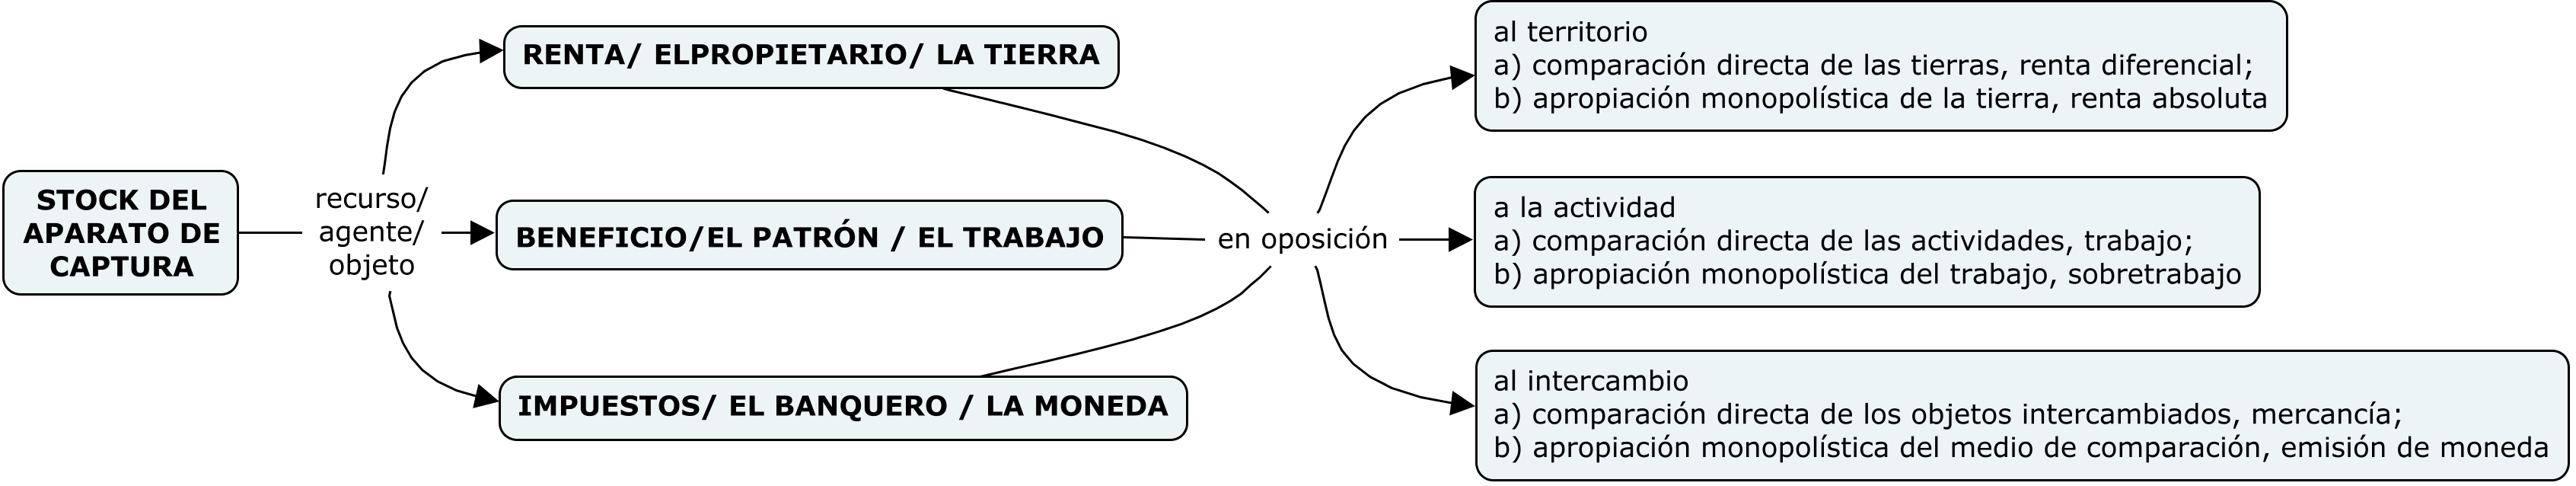
\includegraphics[width=0.7\linewidth]{images/deleuze-captura.png}
  \caption{Estructuras y agentes del aparato de captura.}
  \label{fig:deleuze}
\end{figure}

Por otro lado, la transformación del Estado moderno al Imperio se caracteriza por la sofisticación de los aparatos de captura en arquitecturas corporativas que bien podrían imaginarse como pirámides cristalizadas. Según el colectivo ANON, se trata de un arreglo piramidal donde la jerarquía y el conocimiento de formaciones sociales aumentan conforme se llega al tope de la jeraquía.

\begin{figure}[htb]
  \centering
  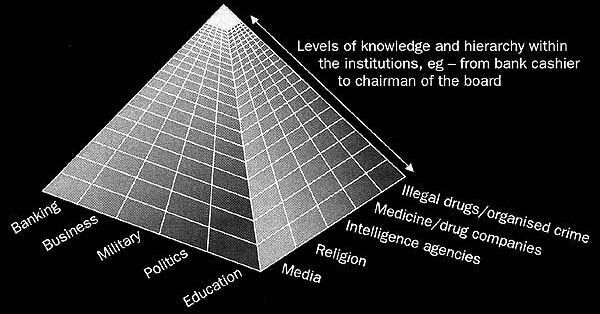
\includegraphics[width=0.7\linewidth]{images/knowledge-hierarchy-piramid.png}
  \caption{Niveles de conocimiento y jerarquía dentro de las instituciones. Ejemplo: Del cajero del banco hasta el presidente de la mesa directiva.}
  \label{fig:hierarchy}
\end{figure}

Al mismo tiempo, proponen una clasificación de los aparatos del Estado contemporáneo:

\begin{description}
  \item[Aparato socio-ideológico:] familia, tradición, religión, nacionalidad, etc. Codifica el deseo y la colonización psicológica del sujeto, establece hegemonía además de producir y mantener el estado actual de las cosas.
  \item[Aparato productivo-comercial:] finanzas, bancos, empresas corporativas, propietarios, etc. Comercialización de la producción, mercantilización del deseo para ligarlo al proceso de producción, monopolización del mercado, el valor de los desvíos que vuelve a los ricos a través de la parasitación de la mano de obra.
  \item[Aparato marcial-carcelario:] los militares, la policía, la inteligencia, el sistema de prisiones. Mantiene el estado actual de las cosas a la fuerza, la disciplina y el control de los sujetos, protege los intereses de los propietarios capitalistas y del Estado, sus fronteras, extrae recursos de otras regiones a través de la fuerza, redirige la riqueza para expandir el brazo militar del Estado e incentiva su investigación y desarrollo.
  \item[Aparato subversivo-periférico:] subjetividades colonizadas, grupos minoritarios, organizaciones criminales, la banda en sombra (\emph{shadow banking}), los mercados negros, etc. Muerte social y necropolítica. Establece la identidad de los ciudadanos mediante la otredad como diferenciación de subjetividades marginales, da un camino al lucro más allá del aparato comercial productivo.
  \item[Aparato legal de la soberanía:] el Estado, el sistema de justicia, los gobiernos, etc. Colonización el espacio geofísico, establecimiento del territorio y determinación de estratos y jerarquías sociales.
\end{description}

\subsection{Un dispositivo es la instancia molecular del aparato de captura}
\label{sub:un-dispositivo-es}

En la introducción planteamos que las resistencias no pueden encontrar soluciones a escalar molar, es decir global. Pese a lo aventurado de esa afirmación, lo cierto es que la vida interior de las resistencias está impregnada de deseo de Estado gracias a que el Estado como categoría del pensamiento ejerce su poder a escalar molar, y también molecular a través de la captura de la técnica política. En relación con el Espectáculo, el teatro de las operaciones del Estado moderno monta escenas, crea situaciones en las que existe una correspondencia entre objetos y su agenciamiento, es decir, aquello que se supone que se haga con el objeto. Un dispositivo es aquel objeto que cumple el fin para el que ha sido diseñado. Es más que una mercancía pues condiciona una respuesta más por una cuestión de diseño que de valor, como ocurre con las mercancías.

Antes de desarrollar los mecanismos del Imperio ---Biopoder y Espectáculo--- tenemos que precisar algunas cuestiones sobre los dispositivos. Dispositivo, según la definición de Foucault es un conjunto heterogéneo, que incluye virtualmente cualquier cosa, lo lingüístico y lo no lingüístico, al mismo título: discursos, instituciones, edificios, leyes, medidas de policía o proposiciones filosóficas. Es también una red de saber/poder, relación entre componentes institucionales. Tiene prácticas singulares cuya emergencia responde a un acontecimiento históricamente particular. Producen sujetos del saber-poder. Es un espacio de saber-poder donde se procesan prácticas discursivas y no discursivas. Producen los objetos de los que hablan (arqueología del saber) y sus regímenes de enunciación organizan las posibilidades de la experiencia (genealogía del poder), de acuerdo a condiciones de posibilidad dadas por la historicidad del acontecimiento. El dispositivo asigna al discurso a un sujeto para que garantice su implementación, en sí mismo es la red que se establece entre estos elementos, siempre tiene una función estratégica concreta y siempre se inscribe en una relación de poder. Es algo general, un \emph{reseau}, una \enquote{red}, porque incluye en sí la episteme, que es, para Foucault, aquello que en determinada sociedad permite distinguir lo que es aceptado como un enunciado científico de lo que no es científico. El dispositivo viene de la etimología \textsc{dis-positio}, \textsc{dis-ponere}. Los dispositivos están siempre en relación con una economía, un conjunto de técnicas para la conducción de instancias. El dispositivo se parece más a una configuración, a una instancia, a una implementación del pensamiento como construcción estriada del espacio. El dispositivo permite gozar de lo abierto como tal, del ente en cuanto ente más allá de la separación de los comportamientos animales de la vida del hombre. A la raíz está un deseo de felicidad. La captura y la subjetividad de este deseo en una esfera separada constituye la potencia específica del dispositivo. Según Deleuze, el dispositivo es una máquina para hacer ver y hacer hablar que se acopla a una historicidad de lo visible y lo enunciable, además de que el dispositivo produce subjetividad.

Para Agamben el dispositivo es positividad, un conjunto de significados impuestos al individuo desde el exterior. Un dispositivo es un ente con capacidad de normar a seres vivientes. Los objetos se vuelven dispositivos en cuanto forman parte de una red de saber-poder. Es un mecanismo que produce posiciones de sujetos por su disposición en red: el individuo es lugar de múltiples procesos de subjetivación. Lo paradójico es el cuerpo a cuerpo entre individuos y dispositivos, pues estos no solo subjetivan sino que producen procesos de desubjetivación, donde la creación de un sujeto implica la negación de un sujeto. Para el autor italiano, se trata de una teología económica y concibe a Cristo como el hombre de la economía (\emph{ho ánthropos tês oikonomías}).  De tal modo ser y acción, ontología y praxis están separadas por una esquizofrenia heredada a la cultura occidental. Bauman ha sugerido que la red que conforma a los dispositivos es un \enquote{sinóptico} que permite a muchos ver a pocos y es matriz donde se procesan a los sujetos consumidores de la sociedad del Espectáculo.

El dispositivo es un régimen social productor de subjetividad, de sujetos sujetados a un orden del discurso o cuya estructura sostiene un régimen de verdad. En la sociedad disciplinaria produce sujetos productores mientras que en la sociedad de control, sujetos consumidores. Todas estas subjetividades se integran según su capacidad de producir respuestas a sus interacciones o estímulos. Sin embargo, la subjetividad que está en disputa bajo el Estado moderno es el \emph{ciudadano-soldado-consumidor-espectador}, que es, en términos prácticos, el policía, el guardián de lo público. Es decir, es una unidad subjetiva modelada a partir del hombre blanco heterosexual con propiedades y en ese sentido construye un sujeto ideal estandarizado. Este sujeto es implementado como ideal a través de la industria farmacopornográfica. ANON propone una clasificación del dispositivo, que define como una disposición, como algo que hace hacer algo a alguna cosa. Sus prácticas son judiciales, tecnológicas y militares:

\begin{description}
  \item[Judiciales:] disponen determinadas \emph{decisiones}.
  \item[Tecnológicas:] los \emph{artefactos} están dispuestos de forma particular en sus piezas componentes o funciones de acuerdo a una disposición particular de estos mecanismos.
  \item[Militares:] ejércitos son dispuestos conforme a un programa estratégico para la \emph{batalla}.
\end{description}

Sin embargo, hay un afuera constituido por todas aquellas formas de vida que resisten a la lógica normalizante del Biopoder. En relación con el Estado, el afuera se encuentra en una reconfiguración del telos del Estado, de la necesidad a la crítica. En relación con las subjetividades, se trata de construir una subjetividad basada en el reconocimiento de la persona como forma de vida.

\subsection{El Estado moderno se vale de un doble monopolio sobre lo político y sobre la crítica, sus mecanismos son la publicidad y la policía}
\label{sub:el-estado-moderno-se-vale-de}

Los mecanismos de operación del Estado son la publicidad y la policía. La policía es la fuerza que interviene donde algo no marcha, donde un antagonismo entre \emph{formas de vida}, un salto de intensidad política ve la luz. La policía ha producido el espacio público como espacio cuadriculado, estriado, por ella. Así, el lenguaje del Estado se extiende a casi la totalidad de la actividad social y se transforma en el lenguaje social por excelencia. Si la política gira alrededor del interés, lo político lo hace sobre el deseo. Si la política es el libre juego del interés común, lo político es más bien el juego de significación de lo común en la vida. Para Rancière, la política va de la mano de la policía, de una forma de garantizar que existan agentes que desplieguen la fuerza física violentamente.\autocite{laclauPopulistReason2005} Tradicionalmente este rol estuvo designado para la construcción del discurso público del urbanismo, práctica de gestión de las urbes. Recursos provenientes de estrategias militares de guerra fueron utilizados para el diseño de la segregación racial en ciudades como Chicago.

La publicidad implica cinismo y la crítica es una forma de publicidad. Pensemos tan solo en el periódico, un medio desde el que podemos expresar diversas cuestiones sobre la crítica. Si el Estado se valió también del monopolio de la crítica es porque la crítica significó durante mucho tiempo lo que Tiqqun llama \enquote{el libre juego de las simulaciones}. La escritura pública, periódica, fue durante muchos años una cuestión propia de los ciudadanos. Es decir, de aquellos hombres que poseían los medios para \emph{hablar}. La publicidad consiste en la participación de los asuntos públicos, urbanos, y es la forma de agencia propia de la ciudadanía. La participación de lo público a través del periódico dió lugar a géneros literarios donde la burla del Yo y la total desconexión entre palabra y cuerpo es más palpable. De igual manera, con el desarrollo del periódico a la radio, a la televisión y algunos años después al internet, la forma que toma la publicidad se torna cada vez más espectáculo, representación convulsa de la imagen, disposición de la mirada al consumo del mundo, a su no participación de él. Así se configura una crítica espectacular, que construye elaborados discursos sobre el estatus quo que terminan formando parte de la industria cultural al no trascender la mera textualidad.

El monopolio de lo político exige también degradar la unidad diferenciada de un mundo en una nación, luego de esta nación en una población y un territorio, desintegrar toda la organicidad de la sociedad tradicional para someter los fragmentos restantes a un principio de organización, y finalmente, tras haber reducido la sociedad a una \enquote{pura masa indistinta, a una multitud descompuesta en sus átomos}, presentarse como el artista que va a dar forma a su materia bruta, y esto por el principio legible de la Ley. Queriendo concentrar el monopolio de lo político, ha politizado todo: todo aspecto de la vida se hizo político, no como contenidos singulares sino que, por la presencia misma del Estado, por su propia presencia, se constituyó a sí mismo en partido \autocite{tiqqunIntroduccionGuerraCivil2008}. En este contexto, la subjetividad que confronta Tiqqun con el Estado, los Bloom, ya no son sujetos, económicos, aún menos que de derecho. Se vuelven criaturas de la sociedad imperial, por lo que deben encargarse de ellos como seres vivientes para poder seguir existiendo \emph{ficticiamente} en cuanto que sujetos de derecho. Una contrahistoria desde el punto de vista de la guerra civil, permite verla como el progreso del monopolio estatal de lo político, victorias ganadas a un enemigo sin historia. La amenaza que representan estos enemigos es la de mundos autónomos, de colectividades no estatales.

El problema del agonismo de Mouffe tiene que ver con su legitimación del Estado y a que es hostil al control estatal, vuelve a plantear un espacio neutro que, sin embargo, siempre es una exterioridad en relación con el vínculo social. Los agentes de policía son aquellos a quienes se paga por consagrar todo su tiempo a cumplir los deberes propios de todos sus conciudadanos. Su misión está centrada en la resolución de los problemas (\emph{problem solving policing}) y preocupaciones de los ciudadanos. Ser policía es, según los grandes estadistas, un arte. De ahí la consagración casi espiritual de la sociedad y de las técnicas que perpetúan su existencia parasitaria. La salvación dejó de estar en el cielo para estar en la ciudadanía, en la entrega absoluta de todo vínculo al interés y a la necesidad. A un policía le encantaría ver cada rincón del universo como un espacio estriado, clasificado, cercado y con una base militar. Nada le causaría más placer que contemplar la metáfora schopenhaueriana de los puercoespines que se cubren del frío a la distancia porque si están demasiado cerca se insertan sus espinas. Y le gustaría verlo en todo el universo, o los multiversos. Es la manifestación de un espíritu totalitario, de una pretensión de reinar sobre todas las cosas, es la aspiración a la totalidad en un cuerpo que se halla alienado de la conciencia, que reconoce el concepto pero no es capaz de experimentar la unidad.

La construcción de la ciudad está relacionada con el desarrollo de la publicidad y la policía. Parece que el Estado, para hacerse más efectivo, se vale de una pragmática psicogeográfica. Es decir, una posición técnica orientada a la construcción de una percepción \emph{pública} del paisaje salvaguardada por un ejército de ingenieros, recaudadores de impuestos, vigilantes y personas dedicadas a la higiene de la ciudad. Pareciera que hay una suerte de similitud, al menos en lo que a públicos respecta, entre los manuales de la policía de Nueva York y los manuales de etiqueta de las cortes francesas en el siglo \textsc{xvi} \autocite{tiqqunIntroduccionGuerraCivil2008}. En relación con la ciudad, la dromología es el devenir arma de los medios de producción, el perfeccionamiento y la maximización de utilidades, la documentación de procesos y procesos de ingeniería iterativa para un balance entre plusvalor y utilidad. Es en este contexto cuando nace el Diseño como una heurística de la producción de mercancías.

\section{En el Imperio, la publicidad muta al Espectáculo y la policía al Biopoder}
\label{sec:en-el-imperio}

En este apartado abordaré algunas cuestiones básicas sobre la teoría crítica sobre el Imperio que desarrolla Tiqqun. Comienzo por la siguiente cita:

\begin{quote}
  Desde su nacimiento, la sociedad mercantil jamás ha renunciado a su odio absoluto de lo político, y es por mucho en esto que reside su mayor contrariedad: que el proyecto mismo de erradicarlo sea \emph{todavía} político. Desde luego quiere hablar de derecho, de economía, de cultura, de filosofía, de medio ambiente e incluso \emph{de} política, pero jamás de \emph{lo} político, dominio de la violencia y los antagonismos existenciales. A final de cuentas, la sociedad mercantil no es otra cosa que la organización \emph{política} de la negación desencadenada de lo político. [\ldots] La doctrina de la utilidad, el sistema de las necesidades, el mito de una autorregulación \enquote{natural} de los mercados, la ideología de los derechos del hombre y la democracia parlamentaria pueden ser incluidos entre los numerosos medios que fueron implementados en ese tiempo, para ese fin. Pero es indiscutiblemente en el período histórico que se abre en 1914 cuando la naturalización de la dominación mercantil reviste su forma más radical: el Biopoder. En el Biopoder, la totalidad social que se autonomiza poco a poco llega a hacerse cargo de la \emph{vida} misma. Por un lado, se asiste a una politización de lo biológico: la salud, la belleza, la sexualidad y la energía movilizable de cada individuo atañen cada año más claramente a la responsabilidad gestionaría de la sociedad. Por otro lado, es una biologización de lo político la que se opera: la ecología, la economía, la repartición general del \enquote{bienestar} y de los \enquote{cuidados}, el crecimiento, la longevidad y el envejecimiento de la población se imponen como los principales capítulos con los que se mide el ejercicio del poder. [\ldots] De lo que se trata en realidad, es de apoyar sobre la falsa evidencia del cuerpo y de la vida biológica el control total de los comportamientos, de las representaciones y de las relaciones entre los hombres, es decir, en el fondo, de forzar en cada uno el asentimiento al Espectáculo por medio de un supuesto instinto de conservación. [\ldots] el Biopoder es esa tiranía esencialmente asesina que se ejerce sobre cada uno en nombre de todos y de la \enquote{naturaleza}. [\ldots] No puede haber política \emph{en el seno} del Biopoder, sino sólo \emph{contra} el Biopoder. Considerando que el Biopoder es la negación consumada de lo político, la política verdadera tiene que comenzar por liberarse del Biopoder, es decir, revelarlo como tal~en~\autocite[Tesis V]{tiqqunTesisSobrePartido}.
\end{quote}

En el Imperio, la norma es el Estado de excepción. Es decir, el destino del Estado moderno no era otro que el de \enquote{nacer como el aparente vencedor de la guerra civil, para después ser vencido por ella. No haber sido más que un paréntesis y un partido en el curso paciente de la guerra civil} \autocite{tiqqunIntroduccionGuerraCivil2008}. La tensión propia del Estado moderno, es decir, su contradicción, yace en que el Estado se mantiene solo por la práctica de aquello que quiere conjurar, por la actualización de lo que supone ausente. Es evidente que la legitimidad del Estado radica de manera efectiva en sí mismo. El Estado en cuanto idea, como Dios, no requiere ningún tipo de justificación para existir. Su ideología es la que inventa las justificaciones como manera de posicionarse más allá de eso que ella misma ha construido. La modernidad creó al Estado y luego a la ciencia para inventar criterios que siempre se ejecutan por las instituciones. La ciencia y todo el discurso tecnocientífico capitalista crean límites, dicotomías, para asumirse como el eje sobre el que gira no solo su visión del mundo sino de lo real. En Tiqqun se plantea el despliegue del poder estatal como una pacificación. El Estado de excepción puede ser descrito como la paz en el Espectáculo, como la invisibilización de un montón de guerras que son libradas para mantener un orden, para contener toda potencia que puede desplegarse al caos, a lo múltiple, a lo íntimo \autocite[pp.~59-97]{tiqqunIntroduccionGuerraCivil2008}. El Biopoder es la sublimación del poder. El Imperio es inmanente a la sociedad, es la sociedad en tanto que esta es un poder. El Imperio tiene sentido solo a partir de la crisis, es decir, como negatividad. La respuesta del Imperio a la crisis es un estado de excepción. Las operaciones negativas, reactivas del Imperio a la crisis, son lo que evidencian su existencia. A diferencia del Estado moderno, El Imperio no niega la existencia de la guerra civil, la gestiona.

El Estado como estado de excepción tiene tanta necesidad de hacerse legítimo como \enquote{la Razón} en un mundo que no pide ser ordenado ni universalizado, que late en la inmensidad del infinito con tal facilidad que catalogarlo como caótico o armónico es una absoluta pérdida de tiempo. Sin embargo, el Imperio no rehúye de la Ley y La Institución. Las ve como armas, pero en realidad no conoce más que las normas y los dispositivos. El Derecho es un arma como cualquier otra en el despliegue universal de la hostilidad. Sin embargo, el Imperio siempre habla el único lenguaje que sabe hablar: el de la eficacia para reestablecer la situación normal, para producir el orden público, el buen funcionamiento general de la Máquina. Lo esencial no reside ya en una proclamación liminar de universalidad. La atención se apoya sobre las operaciones, sobre la \emph{pragmática}. Es una totalización que no nace ya de una voluntad de universalización: se hace por articulación misma de los dispositivos, por la continuidad de la circulación entre ellos. Es decir, del Estado moderno al Imperio, los fundamentos de Ley e Institución se transforman en normas y dispositivos, y la policía y la publicidad en Biopoder y Espectáculo.

En el Imperio, la publicidad se vuelve Espectáculo y la Ley se vuelve norma. La \emph{publicitación} es privatización. Es decir, formar parte del discurso público es formar parte los discursos sobre la propiedad. Es un proceso de despojo donde se otorga a los negocios privados las redes de energía y comunicaciones que fueron construidas con \emph{inversiones} de dimensiones colosales con dinero público. Esa sutileza es lo que rompe el vínculo entre público y común para instaurar un régimen de lo público-privado, que será reforzado por la evolución de la publicidad en Espectáculo. Sin embargo, la propiedad privada también padece una crisis conceptual importante que, no obstante, no tiene implicaciones en la práctica (es decir, en los regímenes jurídicos y políticos). Se trata de un proceso de socialización que favorece al oligopolio de élite. En el Imperio ya no se trata de leyes sino de normas operando como agenciamientos. La norma ignora hasta la idea de una fundación. No tiene memoria, se mantiene en una relación muy estrecha con el presente, pretende desposarse con la inmanencia. En la norma reina una inaprensible instancia de totalización que disuelve, digiere, absorbe y desactiva \emph{a priori} toda alteridad. Bajo el régimen de la norma, nada es normal, todo está por normalizarse. Lo que funciona es un paradigma positivo del poder. La norma produce todo lo que es, en tanto que ella es \emph{ens realissimum}. La negatividad es tan solo un fallo respecto a la norma, un agujero en el tejido biopolítico mundial. Como respuesta, el Partido Imaginario es la sede de la potencia. La razón pública es, nuevamente, un momento, siempre ligado al trabajo, donde se le permite al ciudadano ser escuchado en lo público. Si el sentido común del ciudadano universal es la racionalidad, el mundo de las leyes y de imperativos morales que sirven únicamente como velos de cuanto dispositivo de control ha podido desplegar la sociedad. Esta supuesta racional estandariza todo anhelo y hace utilizable cualquier voluntad para alimentar la máquina de producción de deseo de la normalidad, del Estado para sí.

Habiendo señalado lo anterior, desarrollaremos el Espectáculo como despliegue de la publicidad. Para empezar, el Espectáculo introduce un problema: la dificultad para distinguir el deseo de la obligación. Se impone como obligatorio porque está en posición de ejercer el monopolio visual de la representación legítima. El novedoso principio de control convierte a cada cuerpo en un efecto de iluminación. La subjetividad en la época de la modernización capitalista está vinculada a aparatos modelizadores audiovisuales y estadísticos, propone una paradoja: no deja ver. Propone modos de ver dominantes y señala imágenes-tabú. La visión no es una mera actividad fisiológica social sino también un arte de ver para el cual es preciso educarse. El espectáculo inyecta dosis calibradas de goce y un atisbo del mundo redimido a través del consumo prometido. La esencia de las instancias del espectáculo no está en el análisis de su contenido sino en otras funcionalidades, como una red de relaciones en las que opera y su eficacia para organizar el campo de visión humano. Así, la cartografía territorial deviene atmósfera audiovisual. El espectáculo es una instancia del Estado y es un circuito de observación donde se observa y se es observado. Por ello, el Estado opera iluminando.

Después de las vanguardias, el espectáculo se obligó a renovarse a través de la mostración obscena de sus cimientos. Por ello, la parodia y el comentario infinito sobre sí mismo, además de la incorporación de nuevos productos paraculturales. En la ideología igualitaria del ciudadano se oculta el germen del despliegue masivo de la sociedad espectacular-democrática. La sociedad espectacular regula la circulación social del cuerpo y de las ideas. Nace con la modernidad para dar identidad y unidad a las masas con modelos culturales y funcionales a escala total. Espectáculo es la instauración de nuevas temporalidades y de inéditas topologías espaciales: ubicuidad espacial e intensidad y aceleración temporales, es una crisis de la flecha del tiempo. En todas partes, es diagramación de la mirada y transformación de la velocidad en tiempo inmóvil, el espectáculo es una fe perceptual. La cibernética crea tecnologías y burocracias especializadas en el arte de la vigilancia visual de los cuerpos. La misión de la sociedad tecno-espectacular no está en relación con el progreso sino en conducir a la humanidad a un estadio diferente de dominación, es una \enquote{imagen del mundo deseable}. Las metáforas de las patologías en el desarrollo tecnológico reproducen la lógica de sistemas corporales a las extensiones mediáticas (máquina infectada, contagio, virus). La reunificación de la comunidad es un movimiento inventivo de sí mismo. Y la sociedad comunicacional su negación. Lo que es \enquote{real y experimentable} no puede ser \enquote{representado ni interpretado}.

La cultura espectacular desorganizó la antigua unidad de la clase trabajadora basada en una cultura festiva común. La administración del territorio siempre ha necesitado del arte político, de la desorganización de la comunidad con escribas, burócratas, legitimadores, asesores, parlamentarios). Esto se combate con amistad política. En otras imágenes de sociabilidad nos encontramos con la vindicación de la fiesta y el banquete, y el rechazo a la cotidianidad alienada y al trabajo. El espectador se licúa en una pasividad, crueldad morbosa activa ante la contemplación en diferido de la persecución de sufrientes y perseguidos. Hombres libres son aquellos curiosos que lanzan sondas hacia lo todavía invisible o inaudible.

Lo espectacular integrado es la superación del poder espectacular concentrado (que prioriza la ideología del Estado totalitario como verdad) y el difuso (prescribe la elección deliberada de una variedad de mercancías). Se combinan a través de la renovación tecnológica, fusión económica entre lo público y lo privado, imposición de un verosímil que no admite réplica y la abolición de la memoria histórica, además del exilio de toda forma no espectacular. A estos enemigos se les combate haciendo silencio a su alrededor.

\subsection{El posfordismo es la informatización global del trabajo}
\label{sub:el-posfordismo-es-la-informatización-global-del-trabajo}

\epigraph{\enquote{La tecnología es un discurso sobre las técnicas que no cesa de realizarse. Así como la ideología de la fiesta es la muerte de la fiesta real y la ideología del encuentro es la imposibilidad misma del encuentro, así la tecnología es la neutralización de todas las técnicas particulares. El capitalismo es en este sentido esencialmente tecnológico; es la organización rentable, en un sistema, de las técnicas más productivas. Su figura cardinal no es el economista, sino el ingeniero.}}{\emph{El Comité Invisible} en~\autocite[p.~131]{comiteinvisibleNuestrosAmigos2015}.}

Dicen Hardt y Negri que el declive de la legitimidad de los Estados nación no significa necesariamente un declive en la soberanía. Habría entonces que comprender la evolución de nuestro concepto considerando la nueva dinámica de producción de poder en la sociedad contemporánea. \emph{La libertad se antepone al orden en las sociedades disciplinarias y a la gestión en las sociedades de control.} Esta idea de control reproduce la cuestión de un capitalismo de medidas, de una fase del capitalismo cuyo hito se encuentra en la cibernética como ciencia y arte del control. El Imperio despliega dispositivos de regulación normativa y biopolítica que se extienden hacia muchas partes pero tienen veracidad en cuanto a que producen ciertos flujos de información. Sus aportes permiten entender la cuestión desde una lógica económica. Para ellos, el Imperio es una nueva forma global de soberanía, un aparato de regulación descentralizado y desterritorializante. Cada Estado nación es un Leviatán. La posmodernización de la economía global tiende a la producción biopolítica. Ni Estados Unidos ni otro país están en el centro del proyecto imperialista. El Imperialismo ha terminado. Sin embargo, Estados Unidos tiene fundamentos imperiales, al contar con una constitución formal, compuesta por la Constitución política y otros aparatos legales, y una constitución material, que no es otra cosa sino la formación y reformación de la composición de las fuerzas sociales. Estados Unidos sienta las bases de un arreglo estatal distinto al de los anteriores, donde las contradicciones entre Imperio y República en \autocite[Tratado de Nomadología]{deleuzeMilMesetasCapitalismo2002} fungen más bien como una tensión vital, a diferencia de los arreglos de Europa y su interminable guerra de religiones. \emph{The Federalist}, escrito por Thomas Jefferson, propone abiertamente un concepto, aunque las más despistadas lo miren como una metáfora. Se refiere a un agenciamiento que suspende la historia. Regula no solo las interacciones humanas sino también la naturaleza humana, es la forma paradigmática del biopoder, su fin es la paz perpetua en la historia~\autocite{hardtImperio2005}.

La informatización de la producción está relacionada con el desmantelamiento de la fábrica. Desde su ámbito más productivo, el Imperio puede comprenderse como parte de un proceso económico de informatización de la producción. Hardt y Negri hacen uso de una metáfora sobre la fábrica para explicar las asimetrías históricas entre los países frente a la idea de desarrollo económico. Parten de la premisa de que la producción de un Estado pasa por una fase de agricultura, industrialización y, en estos tiempos, de informatización. A diferencia de lo que predican los apóstoles de la Economía, estos procesos no son escalonados y su anacronismo ignora que hay ventajas permanentes que prevalecen, como el uso político de la palabra, que bien puede traducirse en las capacidades de otros cuerpos políticos para el libre juego de las formas de vida. La cuestión más concreta, en el caso del Derecho internacional tiene que ver con el derecho a explotar la propiedad, extendiéndose ésta hasta el ámbito de los saberes y de las técnicas de exterioridades, que permitan dar más vida, aunque sea artificiosa, al soplo del Leviatán. La falacia ignora que no en todos los países se completa un estadio de modernización (en términos de producción) antes de pasar al siguiente y ofrecen el caso de Italia como ejemplo, que es poderosa en productividad, pero solo en la medida en que conviene a la inversión extranjera. En lo que respecta a las fronteras territoriales, el Imperio las convierte en aduanas-volantes. Un ejemplo claro es el espacio Schengen, que designa el territorio de libre circulación al interior de la Unión Europea. Las aduanas se extienden, en potencia, a todos los lugares y a todos los instantes. A diferencia del Estado moderno, que opera apelando a la Ley y la Institución, el Imperio es el garante de la proliferación reticular de normas y dispositivos. El Imperio calcula, pesa, evalúa y luego decide estar presente en un lugar o en otro. Manifestarse o retirarse en función de consideraciones tácticas. De modo que está en donde podría estar. Se mantiene en cada punto del territorio, en el espacio que hay entre la situación normal y la situación excepcional, puede su propia impotencia.

El Imperio se caracteriza porque su modo de producción da forma a una inteligencia cibernética de las tecnologías de la información y de la comunicación. La consecuencia más importante de esto tiene que ver con una transformación en la concepción del trabajo, que a su vez afecta el modo como se comprenden la tierra y el capital como factores restantes de la producción. Este cambio paradigmático consiste en la transición del fordismo al toyotismo. Por la abstracción del trabajo, fragmentado a través de diferentes actividades, la computadora se propone a sí misma no solo como central sino como \emph{herramienta universal}, a través de la cual pasaría toda actividad. Significa también un trabajo afectivo e inmaterial, que produce redes sociales, comunidad y Biopoder. El trabajo inmaterial del sector de servicios tiene que ver con la manufactura, con tareas analíticas y simbólicas, y la producción y manipulación del afecto a través del contacto humano.

En términos históricos, el futuro del trabajo empieza en Japón. A fines de los años setenta y a lo largo de los ochenta, con el declive del fordismo-taylorismo, experimentamos un auge del toyotismo. Este viraje coincide con el auge de la literatura gerencial y su gran auge como \emph{best-sellers}. Esta forma de literatura narra la evolución y configuración del futuro del trabajo. El sistema de información de las nuevas líneas de ensamblaje, desarrolladas en Toyota por Taiichi \={O}no, plantea una producción en serie distinta al modelo fordista tradicional. La distinción está en el \emph{push-pull}. En la cadena de suministro \emph{push}, o de empuje, la producción se determina por la planeación, mientras que en \emph{pull} \footnote{El sistema Toyota plantea un \emph{pull system}, un sistema de control dentro del proceso de producci\'{o}n que significa solicitar las piezas que se necesitan, cuando se necesitan y en la cantidad exacta necesaria, para evitar mermas.}, está determinada prácticamente por la relación entre oferta y demanda. Esto favorece el proceso de pulverización del ensamblaje de mercancías, simplificando y exacerbando al mismo tiempo la enajenación del trabajador. Este modelo ha mutado para adaptarse a las dinámicas tecnocapitalistas que predominan en el cínico ambiente de la innovación tecnológica, donde abundan las formas cibernéticas de producción y de control colaborativo. El desencanto de la élite neorreaccionaria de Sillicon Valley se exacerba, como hemos visto anteriormente, conforme es más aguda la alienación, mientras más aumenta la capacidad de la tecnología para automatizar tareas.

La fuerza de trabajo es capital variable, una fuerza activada y configurada solo por el capital, porque los valores cooperativos de la fuerza de trabajo, particularmente el trabajo inmaterial, le permite al trabajo valorarse a sí mismo. De modo que hoy, la productividad, la riqueza y la creación de plusvalor toman la forma de una interactividad cooperativa a través de redes afectivas, lingüísticas, comunicacionales y afectivas. Lo anterior muestra de qué modo la dualidad conceptual que existe entre el trabajo y el ocio son síntomas del Biopoder. Los avances de la cibernética desterritorializan la producción dispersando las fábricas masivas, evacuando las ciudades-fábrica, pues para el patrón comienza a resultar innecesario tener una fábrica cuando el \emph{coworking} y las oficinas-café pueden cumplir esa función. La cadena de ensamblaje es reemplazada por redes, sin centro físico o territorial. Dejando atrás los modelos verticales, industriales y corporativos, la producción está organizada en redes de empresas horizontales. La informatización de la producción y la importancia de la producción inmaterial permiten liberar el capital de los límites tradicionales de territorio o de negociación. En clara afinidad con los planteamientos de Paul Virilo, Hardt y Negri apuntan hacia las carreteras como caminos romanos, donde la paradoja reside en que la red en sí misma es al mismo tiempo el sitio de producción y de circulación \autocite{hardtImperio2005}. Así, el Estado moderno logra consolidar la tensión entre Imperio y República a través de un mecanismo democrático, el internet como rizoma, y uno oligopólico, una red de transmisiones y difusión de la industria de la cultura, algo que ellos llaman una nueva estructura híbrida de información-red.

En el posfordismo, la gestión de la vida y la muerte es cibernética, pues nuestro mundo es de redes, navegable a través de teorías de la complejidad y del caos. Muchos procesos automáticos alimentan diariamente el flujo de operaciones de las infraestructuras (redes de abasto de combustibles, electricidad para servidores, satélites, líneas de internet) sin que haya realmente un responsable. Las funciones están programadas y los destinos predeterminados. Miles de variables interactuando entre ellas a partir de distintos nodos que envían información diversa y que demandan u ofertan certificados a través de internet. El propósito de la cibernética es dispersar para crear un caos gestionable, incluso automatizable. Ella condiciona una nueva relación ontológica, un \emph{gestell}, entre las formas de vida y las cosas a través de la imagen, con el auge de la sociedad red y gracias al desarrollo acelerado del internet. Si el Estado moderno reina sobre la república fenoménica de los intereses, el Imperio reina sobre la república fenoménica de las diferencias, es en realidad el libre juego de los simulacros. La idea democrática de la equivalencia entre todas las formas de vida no es distinta de la idea imperial. De modo que la democracia es imperial al establecer la equivalencia negativamente, por el hecho de impedir por todos los medios que las diferencias éticas alcancen en su juego el punto de intensidad en que devienen políticas. La república política es la democracia en el interior de la forma abstracta del Estado. Es por eso que la forma abstracta de Estado de la democracia es la República. En la verdadera democracia, el Estado político (en la medida en que apunta a la ficción de lo Uno real y toma partido por ello, neutralizando su uso metafísico de las técnicas) desaparecería. El capitalismo es el arma técnica-productiva del Estado y el patriarcado el referente simbólico, mientras que el Estado se refiere solo al proceso, es noología ante todo. La cibernética se entrecruza con la inteligencia y la farmacopornografía a través de técnicas masturbatorias, donde toda producción cultural es entretenimiento. Parece que hay una forclusión de la potencia gaudendi (véase~\ref{wrd:potentia}) por la creación de ciertos soberanos legítimos con el monopolio de la excitación.

El arma más letal y compleja del Imperio es la cibernética. Si aceptamos la metáfora ciborg de Haraway y asumimos que somos, al mismo tiempo, organismo y máquina, nuestro cuerpo es complejo entramado de canales y circuitos susceptibles de ser penetrados. Podemos definir a la cibernética como ciencia y arte del control.

La teoría de la información es uno de los elementos centrales de la cibernética. El dominio tecnológico de esta para el mundo yace en la capacidad de instrumentalizar cualquier relación. Entender los circuitos de información se hace clave para ir más allá de la visión tecnologizante de la realidad, para encontrar mecanismos que rompan la lógica de control que se hace cada vez más difusa y permanente dentro de la vida. La \emph{forma de vida} que por su comprensión tecnocrítica del mundo es capaz de desdoblar y visibilizar los elementos que dan poder al Imperio en su despliegue cibernético, es una que deviene hacker. La constitución de una multitud de hackers constituye un cuerpo político pirata. Es necesario que mencionemos que este espíritu es también el más proclive a entregarse al Imperio si este logra sembrar la necesidad en el espíritu. De suerte que el hacker se encuentra siempre en un dilema de acción, pues en cualquier momento puede volverse un policía. Y no solo eso. Es tan fino el saber del hacker que su traición podría significar aumentar su potencia al grado de volverlo un robocop: policía de lo real en el deseo.

La descentralización ha sido una de las herramientas más poderosas e invisibles del Imperio para la difusión de su poder. Hardt y Negri explican cómo la desterritorialización permite que el dominio biopolítico de este Leviatán sea cada vez más sutil. Frente a ello, el paradigma de redes distribuidas se asemeja más a la posibilidad de crear un mundo de autonomía, con saberes relativamente accesibles, donde no hay centros de poder porque todo está, literalmente, en todas partes.

La cibernética nos ha convencido cada vez con menos argumentos y dificultades, de la importancia de vivir siempre a expensas de una moneda con la intención de reproducir el dominio de la Publicidad en toda relación, de tal suerte que el Espectáculo pueda mantenerse como el dominio pleno de lo real. Queda así como un tema de suma importancia la distinción entre lo real, lo virtual y lo digital.

En lo que respecta al deseo, consideremos en principio lo siguiente: el Imperio no solo genera un despliegue biopolítico de poder, sino que también desarrolla, cada vez con más eficacia, una cibernética del deseo. Una de las formas más simples para entender la naturaleza de esta cibernética del deseo la plantea \autocite{preciadoTestoYonqui2008} con el concepto de \setconcept{\emph{potentia gaudendi}}{wrd:potentia}. Esta potencia es una que atañe a la libido y que evidencia de manera concreta la tesis de Deleuze sobre la producción-deseo. Entre otros problemas, uno de los principales desafíos es cómo crear una relación dialéctica entre lo común y lo íntimo que rompa con la lógica de lo público-privado.

Los desarrollos de las nuevas ciencias, en particular en teoría de redes y cibernética nos permiten entender los sistemas de maneras muy distintas y con problemáticas que también difieren. Por un lado, pese al miedo que la izquierda más dogmática y que una misma rama de sombra ludita dentro del anarquismo radical tienen frente a la tecnología y al control, no reparan en que el problema es la tecnología como concepto. En el Espectáculo, en lo que en Tiqqun denominan como época de la indeterminación, del \emph{se}. En el siguiente apartado desarrollaré la cuestión de las tecnologías cibernéticas y su relación con la producción cultural.

\subsection{La industria farmacopornográfica es el paradigma de toda industria cultural}
\label{sub:la-industria-farmacopornográfica}

\epigraph{\enquote{Todas las razones para hacer una revolución están ahí. No falta ninguna. El naufragio de la política, la arrogancia de los poderosos, el reinado de lo falso, la vulgaridad de los ricos, los cataclismos de la industria, la miseria galopante, la explotación desnuda, el apocalipsis ecológico\ldots{} no se nos priva de nada, ni siquiera de estar informados de ello. [\ldots] Todas las razones están reunidas, pero no son las razones las que hacen las revoluciones; son los cuerpos. Y los cuerpos están delante de las pantallas.}}{\emph{El Comité Invisible} en~\autocite[p.~7]{comiteinvisibleAhora2017}.}

La forma despótica del Imperio se caracteriza por una pulverización del poder y un cambio en los modos de producción, donde se privilegian los procesos industriales pulverizados, sin fábricas ni obreros reunidos en un mismo espacio, también por el auge de entidades más allá de los Estados nación, como las empresas trasnacionales, que compran representantes políticos en Cámaras legislativas y parlamentos para legislar en favor de sus intereses. Detrás de cada uno de los aparatos de Estado existen entidades económicas con transacciones y reglas del juego que regulan la vida en diferentes esferas pero a dos escalas, una micro (corporal, que corresponde al Biopoder y el Espectáculo) y macro (burocrática, de legislación e infraestructura tecnológica). En principio, podríamos hablar de las cinco grandes empresas que condicionan el desarrollo de las telecomunicaciones: Google, Apple, Facebook, Amazon y Microsoft (\textsc{gafam}). Estas son la base material por donde fluyen información y códigos sociales, representaciones del mundo, que son reproducidas en los dispositivos personales para provocar una reacción, un deseo. Esta nueva forma del capital explota reacciones, capitaliza el placer que puede cuantificar en \emph{clics} y \emph{shares}.

Este ciclo se basa en un delicado circuito de excitación, frustración y excitación que regula los hábitos de consumo. Se trata del modelo ideal de empresa neoliberal, un paradigma del negocio posindustrial. La pornografía es un régimen estético que produce significados y un modo de presentación de las cosas que resulta adictivo, que permite obtener satisfacción del placer masturbatorio sobre la representación de cualquier fantasía posible materializada en videos.\footnote{De cierto modo, que el capitalismo se presente actualmente en su mayor apogeo a través de la industria farmacopornográfica (régimen toxicológico y semiótico-técnico), reproduce una concepción de la subjetividad como no castrable, cuyo horizonte parece ser el de autómatas dependientes del \emph{soma} de Huxley, personas discapacitadas, incapaces de habitar, de subsistir autónomamente. Cfr. \autocite{preciadoTestoYonqui2008}.} En los foros de internet para varones adictos a la pornografía existe un nombre para el circuito pornográfico que tiene atados a tantos hombres a una forma particular de desear. Se conoce como: \emph{Porn, Masturbation, Orgasm (PMO)} \autocite{NoFapDonLie}. El malestar de estos hombres cada vez más incapaces de vivir y en simbiosis con las comodidades del capitalismo que extienden el poder de sus formas tristes de vivir a otras esferas sociales, son el síntoma de este nuevo rostro de la economía. La excitación, la erección, la eyaculación, el placer y el sentimiento de autocomplacencia y control omnipotente se vuelven materias primas del proceso productivo.

Por esta razón, Paul Preciado señala que la pornografía es el rostro desenmascarado de la industria de la cultura y propone el concepto de \emph{farmacopornografía} para referirse al gobierno biomolecular y semiótico-técnico de la subjetividad sexual. Hay, de hecho, empresas que se encargan de regular la producción de contenidos excitantes que funcionan como mercancías con estudios explotadores y personas trabajadoras sexuales explotadas. La explotación mercantil del sexo es paradigmática porque un solo video puede producir millones de orgasmos \autocite{StatsArchivesPornhub}, lo que contrasta con la industria farmacéutica, donde el desarrollo de un medicamento cuesta muchísimo pero es fácilmente reproducible una vez que se obtiene y patenta una fórmula \autocite{preciadoTestoYonqui2008}. Así, las grandes entidades económicas capitalizan problemas clásicos de la economía como las asimetrías de información, el problema de agencia o los dilemas de acción colectiva. Además, condicionan nuestros deseos imprimiendo en nuestras psiques imágenes de lo deseable, además de crear una erística que nos enseña que esos estímulos que aprendemos a desear los podemos obtener a través de la moneda, de intercambios mercantiles. Estas empresas aprenden a través de costosas investigaciones sobre el comportamiento humano, para reproducir la servidumbre en los contenidos a través de segmentos de mercado donde se puede insertar el discurso del parásito capitalista bajo distintas situaciones y formas sexuales. PornHub es el paradigma de la industria cultural por su capacidad para producir orgasmos, para \emph{gestionar el género, la excitación, la frustración y el placer}. De este modelo de empresa se pueden extender otras versiones blandas (\emph{soft}) que operan en otros aparatos sociales. Por ejemplo, Disney funciona como el dispositivo que reproduce el imaginario de la jerarquía social a través de sus mitos de princesas, reyes y la construcción del otro como monstruosidad. Algo parecido hacen McDonald's y Coca Cola para reproducir la chatarrofagia.\footnote{Es decir, la enfermedad de la impotencia, del cuerpo enfermo, pauperizado, envenenado por las bombas mediáticas que producen la comida rápida o chatarra como lo deseable, como el lugar donde gastar el \emph{salario}. Se trata de un régimen alimenticio de productos vacíos, compuestos de harinas, grasas, sodio, azúcares y otras sustancias que funcionan bajo el mismo principio de estimulación-malestar y que producen serios daños al cuerpo a largo plazo. El paradigma mercantil de la comida en tiempos del Imperio.}

En el Imperio, que es la crisis del Estado moderno, es decir, la crisis de la religión de Estado, el capitalismo se comporta como un virus. El cambio de paradigma de modelos de gobernanza en masa a modelos en red obedece al desarrollo cibernético del algoritmo capitalista referenciado en el diagrama del mismo nombre dentro del texto. Las sociedades disciplinarias y de control son demasiado complejas para gestionar, por lo que es más fácil fijar protocolos para gestionar redes de manera más eficiente. El espacio masivo está condicionado al número de participantes en un espacio y un momento particulares mientras que el espacio de redes se extiende y contrae en el espacio-tiempo de acuerdo a las órdenes y necesidades de la red. Es decir, su uso del capital es más eficiente porque se ajusta a las necesidades de cada momento. La economía posfordista computacional se basa en circuitos de producción de excitación-frustración y el porno es el paradigma de la industria cultural porque permite transformar cualquier pulsión en mercancía capitalizable a través del \emph{tracking} (seguimiento) del tráfico de sus efectos frente a los espectadores. La excitación, la erección, la eyaculación, el placer y el sentimiento de autocomplacencia y control omnipotente se vuelven materias primas del proceso productivo. Los reaccionarios son peligrosos porque son los consumidores y espectadores de la farmacopornografía. Los NRx (NeoReaxionaries) transforman concienzudamente todas las transacciones en utilidad.

Parece que en tiempos del Bloom, donde la neorreacción, el Partido de los agentes del nihilismo, ha tomado posición, la sociedad de control, la del cansancio y la del aburrimiento \autocite{orozcogaribaySociedadCansancioSociedad2015} coexisten de forma simbiótica cuyo eje común es el cobro de rentas de distintas formas de capital. Resulta paradójico cómo los Bloom son quienes más son capaces de reconocer la violencia. La cuestión de la neutralidad es fundamental.* Los aburridos son quienes reconocen la violencia en cualquier \emph{forma de vida}. Forclusión, resentimiento, castración. A ello sumarle la programación de género. La alternativa es el deseo de llegar a ser dioses. Es decir, a sacralizar el cuerpo, a racionalizarlo por completo bajo el discurso tecnocientífico productivista del Capital. Agamben nos permite ver como esto es también la mercantilización, la entrega total del cuerpo al objeto. Bloom es inclinación a la nada, a la paranoia neurótica? A la inmovilidad, a la asfixia. A la incapacidad de actuar por la ruptura primigenia entre acción y vida por la dicotomía moderna entre teoría y praxis. La inclinación a la nada está relacionada con el nihilismo neorreaccionario. La fuerza vital termina en el partido imaginario, como una violencia arrebatada que solo espera resonar, es pura fuerza sin propósito. Es la nuda vida sin agencia. Me resulta prudente retomar la siguiente cita:

\begin{quote}
  \enquote{La antítesis del comunismo no es el capitalismo sino la economía.}\enquote{El Comité Invisible en~\autocite{EconomiaConsideradaComo}}. 
\end{quote}

El Espectáculo es también la instancia psíquica por excelencia del Imperio. De modo que el Espectáculo se erige a cada momento como emperador de nuestros regímenes libidinales, pues de no hacerlo corre el riesgo de reventar. Es necesario que constituya ficciones ontológicas que permitan que la alienación del trinomio hombre privado-singular-social no produzca una esquizofrenia de tal magnitud que nadie crea más en la autoridad del Estado. La industria cultural corporativa también se adapta al posfordismo, donde la pornografía es el paradigma de la industria cultural. El paradigma de la industria cultural corporativa de Disney tiene como finalidad instaurar un imaginario donde predominan fantasías infantilizantes como una forma de reproducir el aprendizaje de jerarquías, de castas y de roles. En ese sentido es que el cinismo y la crítica son publicidad, porque se constituyen como institución, como la instauración de aquello que suponen ausente. En el posfordismo la crítica es espectacular y es pornográfica por la respuesta cognitiva altamente adictiva que produce a través de la representación de imágenes.

Hay un puente económico entre los problemas micro, que impiden a las personas tener agencia, y los problemas macro, que organizan la producción de bienes y servicios. Fronteras entre policía, biopoder y cibernética: la computadora y distinción armas-herramientas. La red es el dispositivo y el Imperio deviene real en sus operaciones. La blanquitud del hombre es la forclusión de la \emph{potentia gaudendi}, el sujeto reprimido sexualmente, los niños rata, reaccionarios resentidos sin poder de excitación, solo pueden ofertar intelecto y deseo de patronazgo (gusto por el patrón, colonizador, etc.). La economía surge para resolver problemas de acción colectiva y el capitalismo es el coyotaje institucionalizado. Una respuesta sistémica debe avocarse a quitar poder y control a las personas que gestionan las asimetrías de información.

La representación es un problema económico que se ha gestionado a través de la política y además de resolverse en la imagen debe resolverse pensando en otros sistemas de gestión de lo político más allá del paradigma metropolitano de lo público. Parece que el horizonte de la estrategia podría tener más sentido a través de paradigmas como \emph{stacktivism} \autocite{brattonStackSoftwareSovereignty2015} frente a una realidad donde nos gobiernan empresas en diferentes esferas, micro (corporal) y macro (burocrático). Las grandes entidades económicas capitalizan los problemas básicos de la economía para reproducir la servidumbre. De acuerdo con \textsc{anon} \autocite{PeopleArePeople2018}, los problemas de acción colectiva que necesitamos resolver para combatir la economía son:

\begin{description}
  \item[Gobierno representativo:] entender a los representantes como traficantes de información sobre los incentivos de sus representados (problema de agencia).
  \item[Burocracia:] cualquier burócrata sabe que una parte importante de la función del gobierno es el procesamiento de certificados y documentos. Una alternativa es pensar que la burocracia sea reemplazada por programadoras que mantengan un modelo de gobernanza como una máquina de información en \textsc{floss}.
  \item[Cambio climático:] un sistema de gobernanza efectivo tiene que permitirnos reconocer los costos reales y las externalidades de la producción para administrarlas en un equilibrio de Pareto.
\end{description}

A partir de estos planteamientos, el siguiente capítulo desarrollaremos la producción de subjetividad del hombre moderno, del Bloom, que en tiempos del Imperio es quien más padece la alienación mercantil, quien más está sujeto a la maquinaria estatal y a sus formas de condicionar el deseo y mediarlo a través de instancias mercantiles.
\chapter{El Bloom es el sujeto económico del Imperio}
\label{cha:el-bloom-es-el-sujeto-económico-del-imperio}

Hasta ahora hemos analizado el Estado desde su devenir molar y las operaciones de sus aparatos de captura y modos de producción a través de máquinas sociales. En este capítulo analizaremos el Estado desde el Bloom, una instancia molecular del Estado que bien podríamos señalar como el hombre-masa, para entender como NRx apela al sentir de esta multitud. La razón por la que escogí al hombre-masa es porque es el sujeto económico del Imperio, la forma-sujeto por excelencia, aquel que está atado a, y por el cual tiene sentido, toda la forma mercantil de aparatos y maquinas. El proceso que a escala molar, toma el aspecto del Estado moderno, a escala molecular, se llama sujeto económico. Designa un proceso de monopolización creciente de la violencia legítima, un proceso de deslegitimación de toda violencia excepto la suya. Su existencia obstaculiza cada vez más drásticamente el libre juego de las formas-de-vida, para extraerles nuda vida \autocite{tiqqunIntroduccionGuerraCivil2008}. En el capítulo anterior expliqué la transición del Estado moderno a su repliegue contemporáneo, el Imperio, así como el desarrollo de la cibernética y de la tecnología como parte del proceso de sofisticación e incorporación de los mecanismos del Estado moderno a escalar molecular y molar. Sin embargo, he hablado poco del malestar que produce el ideal de la ciudadanía y cómo los neorreaccionarios son el síntoma de la crisis de la religión de Estado, que impide a cada persona vivir conforme consigo misma sin desear un afuera, es decir, sin desear espectacularmente. En este capítulo explicaré cómo se produce el resentimiento del neorreaccionario que produce el derretimiento (\emph{meltdown}) que el Comité invisible señala como Bloom, una profunda experiencia de alienación y de nihilismo que invade la vida psíquica de toda forma de vida dentro del Estado. Desarrollaré cómo el derretimiento y la experiencia del Bloom están relacionados con una búsqueda religiosa más allá de la falsa promesa del Estado de totalidad de sentido sobre lo real.

El trabajo es una de las cuestiones clave en el desarrollo de la subjetividad nihilista, específicamente de la ciudadanía. En los siguientes apartados explicaré el papel de la ética del trabajo de la religión de Estado en la configuración de subjetividad del Bloom, una forma masculina que, como veremos, incorpora la falsa conciencia ilustrada. A continuación analizaremos el desarrollo molecular del Estado moderno. Es decir, al sujeto económico.

\begin{table}[htb]
  \caption{Instancias de territorialización a escalas molar y molecular.}
  \label{tab:tablename}
  \centering
  \begin{tabular}{cc}
    \toprule
    \textbf{Instancias del Estado} & \textbf{Escala}\tabularnewline
    \midrule
    Estado moderno & Molar\tabularnewline
    Sujeto económico & Molecular\tabularnewline
    \bottomrule
  \end{tabular}
\end{table}

\section{El rostro contemporáneo de la ciudadanía es el Bloom u hombre masa}
\label{sec:el-rostro-contemporáneo}

El argumento central de este capítulo es que el Estado produce al déspota como representación a desear. Es decir, el deseo de deseo de Estado es también una cierta iconografía, un manual de etiqueta de lo que el déspota hace, de cómo se relaciona con la servidumbre. Lo resumo de la siguiente manera:

\begin{quote}
  \emph{El deseo de deseo de Estado es el deseo del deseo del déspota. Bloom también es apellido del hombre de Estado que vive profundamente frustrado.}
\end{quote}

El Imperio es \emph{kat-echon}: poder histórico que llega a retener el advenimiento del Anticristo y el fin del \emph{eón} actual, como lo señala Carl Schmitt en \emph{El nomos de la Tierra}. El Imperio se aprehende como el último bastión contra la irrupción del caos y actúa dentro de esta perspectiva mínima. El Imperio es la agonía de la civilización. Frente a esta agonía, el Partido Imaginario ocurre cuando el Afuera ha pasado dentro. Es la otra cara del repliegue, en un mundo donde no hay ningún Afuera visible, donde la Gran Locura clásica, la Naturaleza pura o el Gran Proletariado clásico de los obreros pierden toda fuerza de atracción imaginaria. Esto se debe a que hay afuera por todas partes, en cada punto del tejido biopolítico. El Biopoder no rige directamente sobre los hombres o cosas, sino sobre posibilidades y condiciones de posibilidad.

El hombre masa que se vuelve segmentado vive una forma de alienación de forclusión de su potencia gaudendi, de la abyección de sus propios deseos en el espejo de sus pulsiones. Nunca le es posible reconocerse pues no hay un otro, solo hay mimesis del algoritmo que transforma el gusto en capital-clic. El clic es la forma contemporánea del \emph{purchase}, de la información en metadatos producida por una transacción económica. Este poder de configuración performativa y molecular se desenvuelve en circuitos de excitación-frustración como lo define Preciado es profundamente adictivo \autocite{preciadoTestoYonqui2008}, \autocite{anderssonSocialMediaDeliberately2018}. El sentir del Bloom es de aburrimiento. Patrones de conducta del déspota de dominación y servidumbre como codigos programados en procesos exhaustivos de capacitación empresarial y coaching. PNL es un ejemplo.

Adam Curtis muestra en \emph{Century of the Self} la forma como las corporaciones utilizaron técnicas de asociación y practicas psicoanalíticas para dar forma a las relaciones públicas. El libro \emph{Propaganda} de Edward Bernesse fue el primer panfleto de manipulación de masas. En la actualidad estas técnicas se han refinado y sofisticado al grado de llegar a volverse algorítmicas, con un algoritmo responsivo y adaptativo que interactúa con las reacciones de los usuarios. La publicidad instaura el deber, el sujeto de Estado no desea, debe.

\subsection[En el trabajo \emph{sujeta} en las dimensiones\ldots{}]%
{En el trabajo sujeta en las dimensiones libidinal-molecular e industrial-molar del Imperio}
\label{sub:en-el-trabajo-sujeta-en}

\epigraph{\enquote{Cuando el esclavo descontento coge jovialmente el brazo de su
señor, hace sentir la fuerza que tendría su revuelta}}{\emph{Peter Sloterdijk} en~\autocite{sloterdijkCriticaRazonCinica2014}}

Un punto importante para comprender la transformación del Estado-nación al Imperio se encuentra en el papel del trabajo. Por ello, en este apartado analizaremos las condiciones de producción del trabajo del hombre-masa en la era cibernética. Para comenzar, tenemos que recordar que la dominación mercantil tiende a expandir sus dominios a toda área de la vida y al hacerlo vuelve trabajo a cualquier acción sujeta de la explotación. Este proceso está relacionado con la transformación de la subjetividad. No por nada el concepto central de las revoluciones de los siglos XIX y XX es la masa, una subjetividad que experimenta la realidad de la misma manera, a través del \emph{consumo estandarizado}. En este proceso, las vivencias en su forma de experiencias cognitivas dan sentido y estructura a la imaginación, es decir a la máquina deseante que es cada singularidad.

Las imágenes crean vivencias y así se configura una idea del pasado, por ejemplo, a través de Hollywood que nos enseña a desear melancólica o espectacularmente) y del futuro, como el telos apocalíptico de ciudades hiperdesarrolladas basadas en una economía tecnocapitalista. A través de estos circuitos de producción tecno-material es que la explotación se extiende a cada rincón del planeta, deja a su paso desolación y muerte para después reconstruir la \enquote{sociedad} en otro momento histórico, como ocurrió después de Auschwitz, a través de los medios que producen para las grandes audiencias, para la industria cultural.\footnote{Que dan forma a la cultura popular y al espectador televisivo en un circuito que lo posiciona como ente pasivo sentado en un sillón consumiendo comida chatarra.} En términos concretos, la masa es el resultado de un proceso sintético en el que el individuo afronta una situación externa a él, participa en la situación y proyecta la situación en otros individuos que habitan el mismo espacio. Como ejemplo está Disney, que transmite efectivamente el deseo de casta a través de sus figuras de princesas, reyes y caballeros. Para profundizar sobre estos puntos conviene revisar los documentales de Adam Curtis, particularmente recomendamos \emph{The Century of the Self} como genealogía de las formas contemporáneas de dominación e \emph{Hypernormalisation}.

Yo he intentado perfilar a la subjetividad ideal del Estado moderno como un sujeto económico que \emph{debe} ser algo parecido al \emph{ciudadano soldado consumidor espectador.} Solo basta recordar que el antecedente histórico del ciudadano han sido los súbditos, los fieles. Quizá desde ahí se perfila el proceso donde las multitudes devienen siempre masa a través de los aparatos de captura. El lenguaje cotidiano es muy útil para hacernos ver cómo se transmite la deuda en la subjetividad de ciudadano soldado consumidor espectador:

\emph{paga tus impuestos}

\emph{sirve a la patria}

\emph{no te pierdas el descuento\ldots{}}

\emph{ni el siguiente show.}

En esta fórmula todas las personas deben. El deber y la deuda provienen del mismo sentir (y de la misma locución latina \emph{debere}). Sin embargo, la deuda tiene una condición que ha sido entregada antes del nacimiento, como una suerte de fruto por el que hay que pagar con el pecado original durante el resto de nuestras vidas. El ciudadano \emph{debe} pagar sus \emph{impuestos}, el soldado \emph{debe} honrar a la Patria, el consumidor \emph{debe} comprar y el espectador \emph{debe} mirar. La deuda es impuesta a través de la norma, una práctica de consumo y de posiciones constante que difumina la decisión para plantear comportamientos en función de roles de género, de clase, raciales, principalmente. La imagen representacional juega aquí un papel fundamental, pues es parte de la economía que re-produce la jerarquía que da forma y sentido al aparato de captura para capacitar a los agentes que operan la maquina capitalista.

\subsection{Bloom, es decir, el ciudadano soldado consumidor espectador está sujeto a través de la pantalla}
\label{sub:bloom-es-decir-el-ciudadano-soldado-consumidor-espectador-está-sujeto-a-través-de-la-pantalla}

La subjetividad propia del Estado moderno es el ciudadano soldado consumidor espectador. Produce votos, paga impuestos, da vida a la sociedad a través de las mercancías, es parte del ejército de reserva y consume imágenes. El Bloom es el sujeto ideal del Imperio. En cierto sentido, señala Tiqqun, la deconstrucción es una nueva forma de policía, es una continuación de la razón pública, de toda crítica como crítica literaria. Es una simple reacción bloomesca porque deja de ver en lo que se lee algo que pudiera relacionarse con su vida. En cambio, ve en lo que vive un tejido de referencias a lo que ha leído ya. La presencia y el mundo en su conjunto, en la medida en que el Imperio le concede los medios para eso, adquieren para él un carácter de pura hipótesis.

Hay, sin embargo, algo de militante en la deconstrucción, como una militancia de la ausencia, una retirada ofensiva en el mundo cerrado pero indefinidamente recombinable de las significaciones. Y tiene una función política precisa, la de hacer pasar por bárbaro a todo lo que se imponga violentamente al Imperio, por místico a quien tome su presencia como centro de energía de su revuelta, por fascista a cualquier consecuencia vívida del pensamiento, cualquier gesto. El enemigo está presente en todos lados bajo la forma del riesgo. La diferencia entre la policía y la población se ha abolido, pues cada ciudadano puede revelarse como policía. Al comprender esta paranoia resulta evidente cómo la huella digital, el residuo de nuestras operaciones, se revela crucial al ser en todo momento utilizable. Que este registro esté disponible hace de cada gesto una amenaza suficiente.

Por otra parte, el algoritmo capitalista nos produce como si se tratara de una cartografía psíquica. El algoritmo del virus capitalista y el condicionamiento de desarrollo de las tecnologías mediáticas para producir excedentes (y residuos) configuran lo que se espera de las personas individualmente y a gran escala. Los medios configuran nuestra capacidad de practicar nuestro gusto o de devenir personas-masa. Tanto así que si en algún momento hubo revoluciones burguesas fue en parte por la capacidad de \emph{leer la prensa escrita} como criterio de consumo literario común suficiente para dar forma a una identidad colectiva revolucionaria, a una identidad de clase. Con el paso del tiempo, la radio y el cine reconfiguraron el potencial revolucionario de las comunicaciones y nuevas formas de sublevación-represión (o gestión) surgieron. \footnote{Por ejemplo, el radio creó un espacio informacional nuevo por el alcance de las emisiones sonoras y la forma como se reproduce. Este cambio tecnológico transforma el modo de concebir el espacio y lo público. Los situacionistas tienen el concepto de \emph{psicogeografía} para referirse al desarrollo urbano y a sus consecuencias en nuestras formas de desear.} Es necesario preguntarnos hoy en día cómo la cibernética ha transformado el potencial revolucionario de los medios y una cuestión central para entenderlo son los memes.

La transformación de la comunicación por la inclusión de nuevas tecnologías nos muestra cómo una forma mediática representa poder y nos revela el papel clave de los \emph{medios,} pues ellos configuran el espacio a través de flujos de comunicación. La configuración (\emph{setup}) de estas redes de comunicación son un catalizador para el cambio social. Consideremos lo siguiente: en la actualidad, los modelos de masa donde un grupo recibe una sola transmisión son reemplazados por modelos donde el individuo recibe una transmisión única gracias a \emph{algoritmos reactivos} que alteran la secuencia del contenido de las redes sociales y de ese modo individualiza y hace única la experiencia de consumo de cultura. La subjetividad ya no es producida como individuos en serie sino a través de segmentos. En el posfordismo, los medios hacen más efectiva la economía del deseo y el algoritmo que reacciona se torna una suerte de mímesis, de espejo.

Este cambio de paradigma de modelos de gobernanza en masa a modelos en red obedece al desarrollo cibernético del algoritmo. Las sociedades disciplinarias y de control son demasiado complejas para gestionar, por lo que es más fácil fijar protocolos para que se autogestionen redes de manera más eficiente. El espacio masivo está condicionado al número de participantes en un espacio y un momento particulares mientras que el espacio de redes se extiende y contrae en el espacio-tiempo de acuerdo a las órdenes y necesidades de la red. Es decir, su uso del capital es más eficiente porque se ajusta a las necesidades de cada momento~\autocite{PeopleArePeople2018}.

La identidad se conforma a través de una relación mediática que produce subjetividades diferenciadas no a partir de sus estructuras psíquicas y de sus deseos sino de sus intereses. El público, la audiencia, la sociedad, la multitud, se configura mediáticamente. Se comunica a través de ciertas estructuras: impresos, altavoces, pantallas, micrófonos, símbolos, gestos, ruidos, memes, etc. Lo que el capitalismo hace es disponer de estos medios para la apropiación de plusvalor. Por esta razón, toda forma de sublevación pasa por una lógica mediática de reapropiación del valor, pues nada revolucionario puede haber si de su base material se alimentan propietarios, banqueros o patrones. En ese sentido, la neorreaccion del whiteness no es otra cosa más que la contradicción entre la idea de libertad y el conflicto que le produce al Bloom reconocerse como agente del capital. Esa tensión que \autocite{huiUnhappyConsciousnessNeoreactionaries2017}, citando a Hegel, identifica como falsa conciencia ilustrada, como dialéctica entre espíritu estoico y escéptico, es también la tensión del reconocimiento tecnomaterial.

El Imperio se representa a sí mismo con gusto, como una red de la cual cada uno sería un nudo. La norma constituye el elemento de la conductividad social en cada nudo. En ese sentido, cada individuo se vuelve un dispositivo. Antes que la información, lo que circula es la causalidad biopolítica, con mayor o menor resistencia, según el grado de normalidad. Las campañas de sensibilización del Imperio son creaciones de fenómenos y de entramados de causalidades que permiten materializarlo en la sensibilidad social. El principal enemigo del Imperio es el acontecimiento, todo lo que podría pasar y que hace peligrar el entramado de normas y dispositivos. De modo que la soberanía imperial consiste en que ningún elemento del espacio-tiempo, del tejido biopolítico, esté a resguardo de su intervención. Bajo esta lógica, los medios de producción tienden a volverse medios de control, pues el edificio jurídico, reducido a un simple arsenal de la norma, hace de todos y cada uno un sospechoso. Por eso, para mí:

\begin{quote}
  \emph{El Bloom es el sujeto económico del Imperio y la neorreacción su ética.}
\end{quote}

En todo caso, el ciudadano es quien está condicionado a la sumisión en las diferentes esferas de lo social (sic. aparato de captura). Reproduce la deuda que da sentido al modo de producción, el valor en sí, una abyección mercantil que hoy en día son promesas sobre promesas en bonos, \emph{hedgefunds} y cuestiones del estilo. La neorreacción es peligrosa porque sus partidarios, agentes de Edipo, pertenecen a la clase que está en el tope de la pirámide de la jerarquía social. La clase angelical, asexuada, de hombres amantes de la Ilustración y tomadores de decisiones, jugando el rol completo de la ciudadanía, haciendo uso de su plena potencia. Fuerza vital de la ausencia, máquina social de mundos tecnomateriales, con complejos y ahora líquidos mecanismos y aparatos, armas y herramientas, de producción de deseo, son los agentes directos, la \emph{intelligentsia} del Imperio. Consumidores y espectadores de la farmacopornografía. Aquello por lo que lo ausente tiene \emph{sentido}. Son cínicos llenos de amargura por el desencanto de la conciencia de sí. La no-incorporación de totalidad de sentido en la conciencia absoluta. Paranoicos cuyo cuerpo les es otro. Para profundizar, en el siguiente apartado desarrollaré el concepto de cinismo como falsa conciencia ilustrada y haré un breve análisis de su relación con la Ilustración.

\subsection{La falsa conciencia ilustrada, pero triste, del neorreaccionario, revela la crisis de la religión de Estado}
\label{la-falsa-conciencia-ilustrada}

\epigraph{\enquote{Si la consciencia simple exige finalmente la disolución de todo este mundo de perversión, resulta que esa consciencia no puede exigir al \emph{individuo} que se aleje de ese mundo [\ldots] esa exigencia hecha al individuo singular es precisamente lo que pasa por el mal [\ldots] pues el \emph{mal} consiste en preocuparse \emph{de sí mismo} en cuanto \emph{singular} [\ldots]. La exigencia de tal disolución sólo puede dirigirse al espíritu mismo de la cultura}}{\emph{El Comité Invisible} en~\autocite{tiqqunTesisSobrePartido}.}

El neorreaccionario es la falsa conciencia ilustrada. Adquiere e incorpora la crítica de la sociedad de consumo, del Espectáculo y de su miseria. Es un cínico y su conciencia aguda se enorgullece de su perfecta impotencia para cambiarlo, movilizada de manera maniaca contra la conciencia de sí y contra toda búsqueda de sustancialidad. En el límite de la sociedad mercantil, esta se instala en el nihilismo para continuar la lógica del estado de excepción. Y el Bloom es diferente del neorreaccionario en cuanto a que su afección es el nihilismo, lo indispone. Lo que vuelve un neorreaccionario al Bloom no es otra cosa sino que su disposición espiritual toma partido por el nihilismo, por la guerra total contra sí mismo.

El \emph{pathos} del neorreaccionario es cínico. Los cínicos son los dueños del mundo y al mismo tiempo, en su calidad de ser sujetos reales totales, son el modelo de ciudadanía. En palabras de Preciado, su deseo es ser violados, transgredidos. Experimentan lo real siempre como simulacro y lo producen como verdad para la representación de sí mismos: el ciudadano soldado consumidor espectador. En este hecho descansa la contradictoria paradoja de nuestra investigación.

Bajo una cultura policiaca, de la represión y de la vigilancia constante, es decir, bajo los albores del régimen disciplinario, se cocinó una entidad política, la sociedad, que no tiene otro fin más que reproducir, en la medida de lo posible, la lógica necropolítica que alimenta al Estado como instauración definitiva de la monopolización de la violencia. Los ilustrados opinan: En todo lugar donde impera la violencia hay un montón de subjetividades idiotas que no saben lo que necesitan ni lo que desean.

La sociedad implementa dispositivos de sentido que instauran el reino de la necesidad sobre el deseo como lógicas desbarbarizantes. En la Ilustración, la crítica tiene la función de reafirmar el poder del Estado y genera una actitud conformista, como la razón pública de Kant. La crítica significa siempre un conformismo. Sloterdijk comenta que \enquote{el cinismo moderno es el resultado de la crítica ilustrada que al desvelar los supuestos de la llamada falsa conciencia ilustrada termina ella misma por volverse la falsa conciencia ilustrada}. Es decir, la Ilustración, con el giro copernicano de la crítica kantiana, no hace sino reafirmar la metafísica de sujeto-objeto, donde el sujeto es una sustancia total, esencial. La modernidad es ruptura con el saber como cuidado de sí y búsqueda de la buena vida. \enquote{Se produce entonces un vacío donde el sujeto, a pesar de conocer y usar el mundo como medio para sus fines, no se encuentra en él} \autocite{anonimoQuinismoImposibleAcerca2010}. La modernidad desliga lo racional de lo subjetivo. La autodeterminación es borrada por la autopreservación.

La ironía de la razón moderna consiste en que debe controlar la fuerza omniabarcante y estratégica emanada de su propia reflexión. En función de lo anterior, podemos entender al Estado en relación con el cinismo, como la experiencia fáctica y mundana como experiencia propia del sujeto que es desterrada del saber ilustrado y moderno si no está mediada por alguna construcción cientificista o en un discurso universal dotador de sentido. Esto es, sin una cosa como la objetividad, ese afuera que da forma y sentido al proyecto de antropología positiva. De este modo, el pathos se rompe y la \emph{areté} es reemplazada por la praxis. La ironía es el lenguaje del cinismo, la posición burlesca y desinteresada de una clase que desea espectacularmente. La Historia es la suma de narrativas que la publicidad, antesala del Espectáculo, usa para enseñar a desear al público, que es siempre potencia revolucionaria, pero cuyo deseo ha sido embrujado porque, al ser voluntad sobre una imagen dada, comparte con la mercancía el carácter fantasmagórico.

La imagen, como la mercancía, adquiere cierta mística que subjetiva a quien la mira, que hace un giro radical en el que el medio es agente de producción de significados y la conciencia solo una instancia sobre la que vaciar cualquier semántica antropologizante. Así, el nihilismo del espectador no es otra cosa que la conquista definitiva del espíritu, la configuración de una audiencia proletaria trasnacional que desea negarse. El cinismo como forma de vida de la metrópoli es resultado de la ironía de volver a ponerse la máscara que pretendió arrancar al Antiguo Régimen. Sin embargo, el cinismo moderno no es de una máscara identificable sino que es difuso. El cinismo supone un rompimiento entre la reflexión y la existencia, ya que el dato empírico que da dominio sobre la objetividad toma el lugar del saber para la vida \autocite{onfrayCinismosRetratoFilosofos2005}. El orden de la filosofía tradicional provenía de una reflexión por la propia fuerza vital y no en una exterioridad como totalidad plena de sentido. \enquote{Cuando el esclavo descontento coge jovialmente el brazo de su señor, hace sentir la fuerza que tendría su revuelta} \autocite{sloterdijkCriticaRazonCinica2014}. Esta condición transforma toda insurrección en un movimiento de interés, es decir, en un momento económico. Todo se vuelve intersticios de caprichos, insolencias secretas y ventajas propias al amparo de la ley. El cinismo de los de abajo muestra la cuestión del sometimiento por placer, una suerte de adaptación somática al miedo y al dolor.

En realidad, el Bloom se parece mucho al cínico, es un individuo amargado, un tipo de masas. La popularización de la crítica lo afirma como sentimiento. El saber del cínico es instrumentalizado y se vuelve una justificación de todo lo justificable. Ni siquiera el individuo confía en sí mismo pues sabe que detrás de él se oculta un tramposo. Para el cínico, el gozo de la vida se suple por la inquietud \emph{esquizofrénica} que se quiere conocer para dominar y controlar. Se resuelve contra todo positivismo al considerarlo como engaño sin darse cuenta de que el positivismo está asentado en la existencia misma. Se vuelve un monólogo racional y objetivante, se estatuye como una \enquote{doctrina inmoral de inteligencia}, niega rotundamente la vida y la posibilidad al individuo de elegirse un totalmente otro. En última instancia, el cinismo se trata de una configuración particular de la subjetividad, un habitus que deambula entre una profunda necesidad de verdad metafísica y un deseo de Espectáculo. Resulta paradójico que, para mucha gente, aunque el régimen esté mal, no existe ni la más remota posibilidad de pensar en derrocarlo, al menos de desconocer su autoridad. O al menos hay algo, una desobediencia, que \emph{podría ser y no es}. La gente internaliza el Estado. Por miedo. Por tradición. Por temor a lo desconocido. En última instancia, porque la crisis, el Espectáculo, es incapacidad de imaginar. En relación con el Estado moderno, el cinismo es el síntoma de la imposibilidad del Estado de constituir una realidad total, la producción ideal del sujeto de Estado.

Lo que el Bloom \emph{debe} hacer es asumir su rol como agente pero ese hecho le produce un vacío pues niega su deseo y le produce un malestar al concebir la libertad como concepto pero nunca como experiencia. De ese modo su espíritu no puede concebir otra cosa que el resentimiento. La fantasía neoreaccionaria de una utopía tecnocapitalista sería un estadio posterior al Imperio, donde todas las contradicciones del Estado son, finalmente, perfectamente asumidas y asimiladas, para dar forma a una nueva forma de regulación biopolítica en donde las barreras entre biopoder y contrato social han sido totalmente desvanecidas. Es decir, se trata de una sociedad donde la libertad en puro concepto y toda forma de experiencia es causa de pena. Esta condición es descrita en los textos de \#altwoke como ultraedipo, la realización concreta de la transformación de la pulsión en deber puro, en norma plenamente interiorizada.

A diferencia de los déspotas, los neorreaccionarios carecen de verdad metafísica y el Espectáculo los ha excluido porque el whiteness significa la des sexualización y el principio del Espectáculo es la gestión de la excitación. De modo que el neorreaccionario es el Señor, aquel que solo puede relacionarse sexualmente a través del interés. Aquel que no puede manifestar su deseo. Quisiera recalcar la cuestión que señalé en el capítulo 2 sobre el deseo del déspota como una forma paranoica. De ahí que cualquier acontecimiento afuera de la norma produzca una fuerte reacción por parte del Estado. Los Bloom son quienes toman partido por la impotencia, quienes in-corporan la abyección de la impotencia. En ese sentido, la religión de Estado es un culto a la frustración y a la represión, a la supresión de toda potencia vital. Sin embargo, existe de hecho una potencia revolucionaria en el hombre-masa en los momentos en los que experimenta plenamente la alienación a la que se ve sometido, un sentimiento de extrañeza donde lo ajeno deja de pasar desapercibido y se incorpora. Tiqqun señala que de esta potencia surge una fuerza capaz de irrumpir violentamente el orden social. Se trata, sin embargo, de una fuerza destructiva, una línea de fuga en la violencia que permite al sujeto, como una olla a presión, liberar un \emph{tanatos}, el residuo vital que acompaña a la producción a través del trabajo alienado. Se trata, siguiendo a Deleuze y Guattari, de la derrama de anti producción necesaria para reproducir el ciclo del capital.

El Bloom es un sujeto cínico cuyo único deseo es experimentar un acontecimiento, cualquier muestra de vitalidad que, sin embargo, necesitan rechazar con la misma fuerza con que la desean. Su cuerpo no deja de ser texto, crítica, discurso sobre la sociedad. La posibilidad de vivir, de hallarse fuera del régimen de enunciación (es decir, de la necesidad de enunciar, de nombrar, como la paranoia edípica), les está completamente negada. En ese sentido, su experiencia del otro es siempre un racionalismo, siempre está afuera del cuerpo. La experiencia del Bloom en cuanto cínico, esta movilizada de manera maniaca contra la conciencia de sí y contra toda búsqueda de sustancialidad. Los Bloom son la potencia del déspota y los neorreaccionarios son los déspotas ilustrados del futuros que desean conducir la religión de Estado hacia el exterminio.

La mística de la religión de Estado es el deseo compulsivo de metafísica, de unidad, de un cuerpo plenamente \emph{organ}izado. La apuesta religiosa de NRx para el Bloom (amor a la nada más allá de clase, etc., por el reconocimiento de la subjetividad) es el discurso tecnocientífico productivista que lleva a la utopía tecnocapitalista, el Ultraedipo. Bloom es la condición del desolado, de quien ya no cree en la religión de Estado. Los NRx toman partido por una alternativa a un Estado moderno que es un Estado con un proyecto universalista y hegemónico en donde no existe el otro, una igualdad en escenario abundancia-jerarquía completamente pacificado \autocite{fraseFourFutures2011,fraseFourFuturesVisions2016}. El escenario después del Imperio, después del exterminio de la diferencia y la instauración efectiva del reino de lo mismo.

La neorreacción juega en la misma experiencia de \emph{Choose your own adventure} que la política folk, una incompletitud con el espíritu absoluto en la Historia. La fantasía tecno política padece de la visión divina de la caja negra, de la incapacidad de ver cosas en las mercancías. La interconexión digital mediatizada del Capital. Ese es el \emph{pathos} neorreaccionario. Mientras tanto, la militancia se ve enfrascada en la fantasía de la sagrada familia, de la construcción política mercantil y estamentaria, basada en roles con manuales de etiqueta aprendidos performativa y mediáticamente. Para mí, el problema del Comité Invisible es que no es capaz de posicionarse frente al espíritu cínico más que con cierto virilismo. Sin embargo, una cuestión interesante es que las condiciones del espectáculo hacen, al mismo tiempo, más capaz espiritualmente al Bloom. La conclusión de este apartado respecto al cinismo:

\begin{quote}
  \emph{El cinismo es el síntoma de la imposibilidad del Estado de constituir una realidad total, la producción ideal del sujeto de Estado, la manifestación de lo que en Tiqqun se enuncia como Bloom.}
\end{quote}

Pese al espíritu negativo del cínico, hoy hay más herramientas para resolver esos problemas que dan tanta fuerza a los embrujos mercantiles. La profanación de esa utopía tecnocapitalista sería una heterotopía de soberanía tecno política, que solo se puede lograr a través de la \emph{tecnocrítica}. A este concepto dedicaremos el siguiente capítulo. Necesitamos un afuera a la jerarquía familiar que solo es la fábrica de deseo que reproduce la sociedad.
\chapter{La posición tecnocrítica es la destitución del Imperio}
\label{cha:la-posición-tecnocrítica-es-la-destitución-del-imperio}

De Laurentis prefiere el termino tecnología al de género para referirse a las formas de opresión performativas y moleculares que condicionan a las formas de vida a sus roles en la jerarquía social \autocite{preciadoTestoYonqui2008}. En este capítulo tomaremos una aproximación similar, al señalar la violencia desde los procesos tecnológicos que la producen considerando también una aproximación interseccional que parece reificar las subjetividades en procesos descriptivos donde las relaciones de género, de clase, raciales o coloniales ejercen el mayor poder descriptivo para analizar las formas de opresión. Si hasta el momento he tratado de explicar algunos componentes generales de la religión de Estado, en este capítulo analizare la cuestión de la guerra civil y la violencia desde sus tecnologías con la intención de proponer una alternativa al Estado moderno que al mismo tiempo sea capaz de responder al problema que según Tiqqun da origen al Estado, que es la guerra de religiones. Si decidí abordar la neorreaccion ha sido porque la cultura de blancos (\emph{whiteness}) profesa el nihilismo pero también posee el estatus de los agentes del Estado. Son propietarios, banqueros o patrones condenados a la misma cultura de hombre-masa que imponen a las personas que trabajan para ellos. En el vocabulario hacker se llama \emph{white hat} o sombrero blanco a los sujetos que practican el hacking, es decir, la intrusion o modificacion de codigos, con fines corporativos o legales. Podríamos decir que son los agentes del Estado con capacidad para desempeñar un papel propio más allá de la norma de su propia jerarquía. Es decir, aquellos con la capacidad de asumir una personalidad más allá de sus condicionamientos performativos y moleculares. Paradójicamente, son también aquellos que a partir del reconocimiento de su nihilismo son capaces de conjurar un afuera a la dominación mercantil por su posición tecnomaterial en la \emph{societas}. En este momento de la Historia tenemos lo necesario para implementar una economía pos-escasez. Se trata de intervenir estratégicamente en esas redes de información, que también son flujos de sentido, producciones de deseo. La utopía robótica tecnocapitalista es una de las aristas de distintos escenarios posibles planteados en Four Futures, donde señala que viviremos en un mundo materialmente condicionado por dos aristas, una de igualitarismo-estamentalismo (o sea, donde las jerarquías manden) y otra de abundancia (por la automatización tecnológica) o escasez (por nuevas formas de los patrones para crear valor explotable). De esos casos, los más extremos parecen ser el mundo donde quepan todos los mundos, sostenido por una infraestructura tecnológica común, y el exterminio, la utopía tecnocapitalista para 1~\% de la población global.

Las cuestiones estructurales afectan por una cuestión de origen, de diseño, sobre las tecnologías que configuran nuestra realidad. El capitalismo, objeto vacío, sustantivo que, al no tener una sustancia definida, concreta y subjetiva, se toma por la derecha como algo que no existe materialmente, sí existe y es un espectro psíquico. Para entenderlo, tenemos que comprender las diferencias entre Estado y Capitalismo en la historia y cómo funciona a grandes rasgos el panorama político a partir de estas diferencias. Sin embargo, el pensamiento del estatus quo es realmente poderoso en cuanto a que el Estado dispone de manera muy particular de los objetos como armas y herramientas que reproducen el modo de producción capitalista.

La capacidad del Espectáculo contemporáneo de producir deseos es extremadamente sutil pero molecularmente brutal. Se combina con el Biopoder, que es molar y molecular, configura su propia ecología a partir de cosas y de deseos. Estas performatividades son tan evidentes que, en términos de género, la forma patriarcal del Espectáculo condiciona al hombre al Bloom y a la mujer a actuar como la princesa a ser salvada.\footnote{Tiqqun intenta hacer un análisis de esta condición opuesta al Bloom en \autocite{PrimerosMaterialesPara}. Recomiendo ver la serie de conversatorios de Leonor Silvestri titulados Teoría de la mala víctima.} Hoy en día, la cuestión se trata de una agresiva campaña por captar la atención de las personas para enganchar sus deseos \autocite{fernandez-savaterAusentarseCrisisAtencion, lanhamEconomicsAttentionStyle2007}. La industria cultural de internet o FAAMG, es decir, Facebook, Amazon, Apple, Microsoft y Google, invierten millones de dólares para programar micropolíticas de género, comportamientos y sustancias, es decir, son artífices de un proyecto capitalista de construcción de subjetividad. En el siguiente apartado trataré de plantear qué sentido tendría un Partido en tiempos donde los mecanismos del Imperio operan con toda libertad y sin que nadie pueda detenerlos \autocite[p.~52]{comiteinvisibleAhora2017}.

\section{Un Partido sólo tiene sentido si conduce a la destitución del Imperio}
\label{sec:un-partido-sólo-tiene-sentido-si}

\epigraph{La guerra es la eventualidad suprema.}{\emph{El Comité Invisible} en~\autocite{comiteinvisibleTeoriaBloom}.}

\subsection{El Partido imaginario se constituye del Bloom}
\label{sub:el-partido-imaginario-se-constituye-del-bloom}

Este apartado es un análisis centrado en las Tesis sobre el Partido imaginario. De acuerdo con Tiqqun, el Partido imaginario es la forma de la Contradicción en la dictadura de y en la visibilidad. Es decir, del Espectáculo. El Espectáculo hace invisible la negación. Se compone de la multitud negativa de los que no tienen clase y no la quieren tener, de la no-pertenencia a la sociedad mercantil. En lo que respecta a la relación entre el Partido imaginario y el Espectáculo, la multitud de clase se configura del siguiente modo: el Espectáculo y el Biopoder buscan apoderarse de todo a través de la lógica de la representación. Busca romper la posibilidad de un afuera y recurre a cualquier ficción, como la Jovencita. Desde el punto de vista del PI, la ciudadanía es la dictadura del deber abstracto de participación en una totalidad social atomizada. La multitud de los indiferentes se vuelve entonces multitud de las personas rebeldes, \emph{Waldgänger}. En el Éxodo se dibujan sentimientos que hacen que la oposición formal entre Espectáculo y PI se vuelva concreta \autocite{tiqqunTesisSobrePartido}. De lo marginal esencial se genera una pertenencia a la no-pertenencia, una comunidad del exilio. La fuga se vuelve estrategia, la política suprema. No existe crisis sino la omnipresencia del P.I., que no tiene centro ni circunferencia pues opera en el mismo territorio que el Espectáculo. La amenaza del Espectáculo no es otra cosa más que sus artífices y trabajadores alienados. Hombres sin aliento, que se juran mutuamente igualdad y respeto pero profesar un profundo deseo por escapar a todo.

El \emph{Waldgänger},\footnote{Este concepto está basado en la obra \emph{Eumeswill} de Ernst Jünger, donde desarrolla el perfil del \emph{anarca}, que se distingue del anarquista por su carácter radicalmente solitario y escéptico \autocite{jungerEumeswil2011}. } aquel que se descubre viviendo en el bosque de sí mismo y es capaz entonces de recuperar la soberanía sobre sí, es una de las formas del Bloom, que hoy en día se encuentra más dispuesto a la destitución pues ha sido expurgado de la sociedad y en su nihilismo, es incapaz de participar del arreglo mercantil. Los neorreaccionarios son el momento en que el Bloom toma partido por el resentimiento y por el nihilismo, para hacer reales y concretos el tanatos que despierta en ellos la alienación mercantil y el rechazo social por resistirse a participar del deseo social. Como la frase de un gangsta en Ocuppy Wall Street

\begin{quote}
  \enquote{Hi! What' s up? My name is Mike. I'm just a gangster from Harlem. I hate my life. Fuck my boss! Fuck my girlfriend! Fuck the cops! I just wanted to say: I'm happy to be here, with you all.} \autocite{comiteinvisibleNuestrosAmigos2015}
\end{quote}

La política masculina reproduce un modelo de activismo \emph{Choose your Own Adventure}. Es la cualidad del héroe, del Ulises desesperanzado porque sus deseos de gobernar han sido aplacados por los sillones de diseño o el espacio público diseñado para alejar a la gente de la calle, por una civilidad autoimpuesta. El Bloom es en realidad el más \emph{sujeto} al Estado, es quien da sentido al mito del Héroe, a la construcción de una Gran Historia Universal o de Una Gran Conciencia. Lo que en \emph{Introducción a la Guerra civil} denominan como la necesidad del Uno, de Dios, de la Razón, de La Ciencia. En las \emph{Tesis sobre el Partido imaginario}, el Comité Invisible menciona que el Biopoder es un momento del Espectáculo. El Espectáculo tiene que ocultar la violencia que implica reconocer que su proyecto es un proyecto meramente metafísico. No se reconoce por el temor que el Espectáculo tiene al vacío. El Espectáculo tiene una campaña de pacificación de las sociedades y de neutralización de sus contradicciones. Su campaña de pacificación es todavía una guerra, pero se reemplaza el tema de la guerra en el lenguaje. Se habla, ante todo, de \enquote{procesos de paz}. En mis palabras, la tesis ocho señala que masas de hombres silenciosos se preparan para el éxodo, rechazan participar en todo lo que tiene que ver con el mundo mercantil. Se dibuja un ethos, un mundo infraespectacular que parece un crepúsculo pero es en realidad un alba, parece una experiencia masiva de la ilegalidad y la clandestinidad. El ocaso compuesto de parches es el espectáculo grandioso y mortal que se devela a quien se atreve a considerar su tiempo desde el punto de vista de su negación, es decir, desde el punto de vista del Partido Imaginario. La noción del PI vuelve visible la nueva configuración de las hostilidades; reivindica lo que conspira por la destrucción del orden presente y el desastre es su obra. El PI es el espectro de lo otro, en una sociedad donde la alteridad ha sido suprimida, es el otro nombre de la paranoia, de la enfermedad de los poderes. En el Imperio como fase terminal del Estado moderno, éste no habla más que de terrorismo, delincuencia, criminalidad, pero nunca del PI. \autocite{tiqqunTesisSobrePartido}.

El estado actual de los Bloom es la toma de Partido por una forma de terrorismo organizada que tiene por objeto hacer efectiva una sociedad donde el otro es plenamente un objeto. El nihilismo espiritual del Bloom es también una condición psíquica caracterizada por la marginalidad y la completa desconexión entre mente y cuerpo, el síntoma de la no-sexuación del hombre blanco heterosexual, de la cual los \emph{incels} (\emph{involuntary celibates}) son el principal exponente. La comunidad de célibes involuntarios son el caso extremo de un estado de resentimiento, frustración y de mala conciencia frente a las mujeres y al feminismo en general por ser una militancia en contra de la objetivación sexual de la mujer ---y del otro en sus diferentes formas. Se trata de comunidades de hombres militantes contra el feminismo y que construyen espacios de odio contra cualquier forma de vida distinta, pues el mero hecho de su existencia representa la arbitrariedad de la metafísica de la nada propia del Bloom. En el artículo de Villodres señalan que convertir a \enquote{la otra} en algo objetual e identificarla como un \enquote{no yo/no igual a mí} es un un pensamiento común entre las personas reaccionarias y fanáticas \autocite{villodresQueSonIncels2018}. Yo añadiría que esta disposición reaccionaria no solo construye a la otra como un objeto en términos de género, sino que construye a toda diferencia como un objeto frente al cual es \emph{deber} adoptar una postura hostil.

Sin embargo, la fuerza espiritual y sexual del Bloom tiene alternativas más allá de la neorreacción como partido del resentimiento (cuya agenda es el totalitarismo urbano tecnocapitalista). La guerra contra la dominación mercantil y contra la religión de Estado solo podrá encontrar victorias allí donde la acción se dirija a la disolución misma del que es/tá \emph{sujeto}, a la \emph{destitución} tecnomaterial del estado actual de las cosas. Una toma de partido por una acción libertaria, tecnocrítica.

\begin{figure}
  \centering
  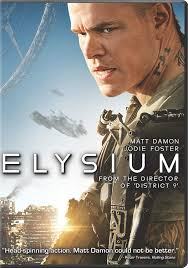
\includegraphics[width=0.7\linewidth]{images/elysium.png}
  \caption{Cartel de la película Elysium, que muestra una tecnoutopía lunar semejante al escenario de exterminio descrito en \emph{Four Futures}.}
  \label{fig:elyssium}
\end{figure}

\subsubsection{¿Una hegemonía del sentido común?}
\label{una-hegemonía-del-sentido-común}

Hardt y Negri señalan que participamos en un momento más radical y profundamente comunal que nunca en la historia del capitalismo, produciendo medios de cooperación y comunalidades comunicativas gracias a la interconexión global producida por internet. El negrismo tiene la esperanza de un Estado democrático mundial. Para el Comité Invisible, sus seguidoras se comportan como si no entendieran que dentro de los edificios pomposos frente a los que acampan no hay realmente nada. Toda la visión negrista se encarga de forzar al Imperio, a través de la emergencia de una supuesta \enquote{sociedad civil mundial}, a darle la forma a un Estado universal. Que esto no nos engañe, señalan. Si bien el Imperio tiene una fachada institucional, su realidad efectiva permanece concentrada en la policía y la publicidad mundiales, que por sus capacidades son ya Biopoder y Espectáculo \autocite{comiteinvisibleNuestrosAmigos2015}. Las intervenciones militares de los países progresistas no son el avance de un derecho mundial naciente sino la subordinación del orden jurídico al estado de excepción policial. Frente a ello, resulta más fructífero devastar al Espectáculo y al Biopoder que militar en favor de un Estado universal salvador.

Diré algo para provocar a las personas afines a la teoría populista que pugna por la hegemonía del \enquote{sentido común}: si recordamos que el Partido imaginario es el motín, siempre presente, del proletariado global y que su existencia evidencia, junto con el cinismo, la fragilidad de los planteamientos que dan forma al Estado moderno, la dialéctica entre constituyente y destituyente es un falso dilema, pues ambas forman parte de una dialéctica de la acción, una tensión entre dos formas de \emph{praxis}. Además del sentido común como lo plantearían Laclau y Mouffe \autocite{laclauRazonPopulista2016}, también se trata de una hegemonía tecnomaterial, como lo han defendido Srnicek, Williams y Hester [@\autocite{hesterXenofeminism2018}] . Para mí, las posibilidades de la acción crítica apuntarían a una pragmática \emph{Free Libre Open Source Software (FLOSS)}, una etiqueta que en la jerga de programación se refiere a la creación de códigos completamente abiertos, manipulables y anticapitalistas. Mientras que la tecnocrítica se ocuparía del develamiento de los dispositivos de poder y al diseño de un porvenir poseconómico.

\subsection{¿Necesitamos más manifiestos políticos?}
\label{necesitamos-muxe1s-manifiestos-políticos}

Al analizar los manifiestos de Maquiavelo y de Marx y Engels, Hardt y Negri señalan que todo manifiesto político efectivo se posiciona sobre un sujeto, que para ellos es la multitud, y un objeto, la liberación cosmopolita dentro del abismo de la posmodernidad \autocite[p.~64]{hardtImperio2005}. Al respecto, considero que las formas de vida configuran el mundo a través de su deseo y de su capacidad de accionar para hacerlo efectivo. Hay que analizar \enquote{la multitud} y la \enquote{liberación cosmopolita}, es decir, determinar un sujeto que acciona.\footnote{Que para mí sería algo así como las formas de vida se posicionan por una areté tecnocrítica.} Analicemos un poco estas posibilidades en medio del debate sobre el Partido y el poder constituyente.

En primer lugar, la multitud es un sujeto social activo que parte de lo común, de las singularidades. No se funda en la identidad, ni en la unidad sino en lo que hay en común \autocite[p.~128]{straehleDIFICULTADESMULTITUDDISCUSION}. Está opuesta a la soberanía, propugna por horizontalidad, es el ensamble de lo singular en lo colectivo sin desembocar en una abstracción genera. De igual modo niega los flujos de poder. Son singularidades que abolen la identidad, no son individuos \autocite{hardtMultitudGuerraDemocracia2006}. Esto emerge gracias a los procesos sociales colaborativos de la producción. Se pasa de la \emph{res pública} a la \emph{res communis}, plantean la asunción de un interés o voluntad general. Esto para alcanzar una libertad más allá de las identidades. Esta subjetividad política está en respuesta al trabajo inmaterial (posfordismo) en una época donde el capitalismo evoluciona a capitalismo cognitivo. La incorporación de la multitud a la política es indeseable pero necesaria. Su concepto de multitud viene de Spinoza. Hardt y Negri argumentan que la multitud no es un concepto sino una realidad nueva. La apología de la multitud conlleva el deseo de que la realidad adopte los flujos históricos del capitalismo como respuesta política. Se prescribe el síntoma como la estrategia última. La multitud está encerrada en una política de mínimos, de un denominador común irrebasable, que alcanza resultados para la unión en la protesta pero no en la construcción.

El problema de la multitud es su indefinición. No se puede saber la orientación que tomará este grupo, o que reproduzca la fuerza capitalista, esa es la cuestión que trae a colación Žižek al preguntar:

\begin{quote}
  \enquote{¿Qué haría este proclamado nuevo sujeto, \enquote{la multitud}, una vez en el poder? ¿Cómo funcionaría el movimiento antiglobalizador reunido en Porto Alegre, ese conjunto de agencias y posiciones políticas incompatibles entre sí? ¿Cómo podrían convivir los granjeros que reclaman proteccionismo con los grupos de derechos humanos y los representantes de los intereses de los inmigrantes que pelean por una mayor movilidad global? Esta lógica de multitud funciona porque estamos hablando de resistencia. Sin embargo, ¿qué pasa cuando \enquote{tomamos el poder}? --si es que éste es realmente el deseo y la voluntad de estos movimientos--. ¿Qué sería una multitud en el poder?}~\autocite{zizekRevolucionBlanda2004}.
\end{quote}

La cuestión es que la multitud solo se define como negatividad a algo. Tiene una tendencia igualmente reaccionaria que parece ignorar las capacidades del poder contrarrevolucionario del Imperio. La multitud fracasa por la tiranía de la no-estructura @TyrannyStucturelessness, pues la potencia para lo común es distinta a la potencia de lo común. Es decir, una multitud que reacciona hacia un \emph{interés común} no es lo mismo que la producción deseante en comunidad y en ese sentido, la multitud carga en su génesis, el interés común, el origen de toda \emph{societas}, de todo contrato social moderno. El concepto de multitud abarca a todos aquellos cuerpos políticos que desde afuera demandan soberanía sobre dispositivos que el Estado ha reservado para sí en cuanto órgano que monopoliza la violencia. Estas multitudes son identidades políticas rizomáticas y solo por poseer esta característica representan una amenaza para el Estado: su hábitat es la heterotopía foucaultiana.

Hay una multitud, constituida realmente como clase, cuya potencia nuclear representa la amenaza más peligrosa para el Estado: la multitud de lxs nadie. Si, como lo señala el Comité Invisible, la economía, la cibernética y la inteligencia son las nuevas bases del Estado como control, el Partido imaginario representa la amenaza más terrible por una razón: el capitalismo basa su dominación sobre el mundo a través de la métrica, de la categorización total del mundo, y el grado absurdo de improvisación, la pureza que proviene de una ausencia de necesidad y de deseo, convierte a estas formas de vida en latencias tan inestables que podrían, de un momento a otro, contaminar cada circuito de este gran sistema complejo de La Necesidad \autocite{EconomiaConsideradaComo}. Todas aquellas formas-de-vida que puedan constituirse de tal modo que su puesta en escena muestre al otro la facilidad de destituir el mundo a través del acto creativo, serán aliadas silenciosas de lo que Tiqqun denomina el Partido imaginario. La multitud, cuya configuración siempre es en torno a una identidad, es un nodo abstracto y su salvación está solo en su capacidad de reconquistar el territorio que, quizá sin saberlo, habita en el imaginario. En la tesis VII señalan que el Partido imaginario es el partido de lo político, toma como foco de la sociedad el trabajo metafísico de una hostilidad absoluta. Por tanto, toma el camino de la \enquote{política absoluta}. Es la forma de lo político en el colapso de los Estados-nación, donde lo político es el elemento total, existencial, metafísico, en el cual se mueve la libertad humana.

Incluso la multitud como subjetividad parece ser otro alcahuete del estado de las cosas. Citando al Comité Invisible: \enquote{El liberalismo existencia ha propagado tan bien su desierto que al final hasta los izquierdistas más sinceros enuncian sus utopías usando sus mismos términos.} \autocite[p.~23]{LlamamientoOtrosFogonazos2009}. Siguiendo a los aceleracionistas de izquierda, creo que ni la Ilustración ni el progreso tienen significados definitivos. Todo el tiempo se constituyen como conceptos en disputa y sobre los motivos de su apropación debería tratar un manifiesto político contemporáneo. Es necesario, en principio, recuperar un concepto de la libertad. Srnicek y Williams insisten en pugnar por la libertad sintética, que es libertad para, potencia y capacidad de acción \autocite{srnicekInventarFuturoPoscapitalismo2017}. Yo añadiría que al mismo tiempo que es libertad-para, es liberación-del yo, del ego, del sujeto. Para mí, la libertad es en parte la renuncia, la deserción a la máquina social de producción deseante y de la economía que sostiene la explotación planetaria de las formas de vida.

En lo que respecta a los temas, habría que imaginar un manifiesto político al alcance de la \emph{complejidad} de nuestros tiempos. Rescatando las enseñanzas de Haraway y de Preciado sobre la construcción molecular del género y las tecnologías de dominación, todo manifiesto, político o no, debería comenzar por situarse. A mi parecer, los planteamientos del Partido y el Poder constituyente tienen, por un lado, el optimismo de los dúos dinámicos Hardt-Negri y Srnicek-Williams, y algo que recuerda a la disputa por el sentido común de Mouffe para ganar los conceptos de universalismo y darles un sentido de libertad positiva, s\autocite{srnicekInventarFuturoPoscapitalismo2017}, libertad-para.

Creo que todo manifiesto político debería posicionarse también frente a los problemas económicos que dan origen a la dominación mercantil. Entre los retos del futuro también se encuentra el hackeo y destitución de la forma jerarquizada y tributaria. Una posibilidad está dada por \emph{commons}, cooperativas y blockchain, además de la construcción de proyectos culturales utópicos que todavía nos acercan a la política representativa de los ideales, donde la imagen todavía está separada de la vida que la produce, que la imagina en acciones concretas, en proyecciones económicas.

En relación con el maniqueísmo colonizador de izquierda y derecha, espectro heredado de la revolución francesa, creo que la bandera contemporánea, pese a la sospecha de la Teoría Crítica más tradicional, más óptima es la disputa por imaginarios sobre libertad pero también sobre el progeso, que para mí es un concepto de fe en la acción para el otro. De hecho, Kant argumenta que se puede creer en el progreso en la medida en que uno es parte de él. No es una certidumbre histórica sino una \emph{disposición}, un principio instrumental para guiar nuestra moral hacia el otro, hacia su libertad. Como lo señalan las xenofeministas, es verdad que la racionalidad es una empresa patriarcal pero eso no significa que tiene que ser así. El estado universal es el reino de Dios en la tierra pero el proyecto de Estado universal puede adquirir otro significado que pelee, por ejemplo, por la hegemonía tecnomaterial xenofeminista.

De igual manera, el manifiesto tiene que considerar la cuestión urbana. De Kant rescato la necesidad de reflexionar sobre el cosmopolitismo, que es una experiencia de clase. La experiencia de la ciudad es la experiencia del consumo privado \autocite{consejonocturnoHabitarMasFuerte2018}, pero eso no significa que deba ser así. Este escenario también puede ser el punto de partida de una destitución de los comunes, de un devenir hacker, de prácticas como lo que el situacionismo francés llamaba psicogeografía o a lo que Virilo se refiere como dromología.

\subsection{Las posibilidades del Partido en tiempos del Imperio se encuentran en plataformas para la destitución}
\label{sub:las-posibilidades-del-partido}

Entonces, estamos en el entendido de que el exterminio es el peor escenario y el comunismo el más impensable. Asumamos que un Partido poscapitalista tendría que buscar conseguir una hegemonía como forma ultima de la acción crítica. Para las populistas Laclau y Mouffe, se trata de construir una hegemonía del sentido común. Sin embargo, recalcando la ironía de la frase de Séneca, señalar el camino no es lo mismo que caminar hacia donde nos conduce. En ese sentido, ¿cómo puede responder el partido a la religión de Estado, fundamento mismo de la modernidad? ¿Sería posible una militancia más allá del cinismo de la crítica? Para mí, el proyecto populista no puede ser una instancia real del Partido Imaginario porque reproduce el deseo de Estado, es su reafirmación.

La falsa dialéctica por identidades revolucionarias, la oposición entre multitud y pueblo se rompe si pensamos en el pueblo como una multitud dispuesta a la destitución. El tipo de Partido para el cual tendría sentido un proyecto destituyente se parece más a una plataforma que a una estructura partidista, como lo rescata el manifiesto Xenofeminista @cuboniksXenofeminismoPoliticaPor. Se trataría de una plataforma política que determine cauces para producir deseos que recodifiquen las huellas psíquicas del Estado. Lo que para Nietzsche es la mala conciencia, para Freud la latencia y para Marx el modo de producción asiático como paradigma de la producción despótica. Esta plataforma debería pensar en los objetos desde su producción, desde su dromología para entender cómo se disponen como armas o herramientas, analizar su potencia tecnomaterial.

En ese sentido, mi idea del Partido supone el desarrollo de una ética de la acción que haga frente a la banalidad de la multitud como subjetividad política y a la tiranía de la falta de estructura. Desde un punto de vista tecnocrítico, mientras la estructura mediática de estas comunidades todavía dependa de aparatos de captura estatales o se inserte en la maquinaria capitalista, ninguna estructura social será capaz de trascender las latencias sobre el deseo que condicionan a una organización a devenir patriarcal o corporativa.

\emph{El Partido debería trabajar sobre la constitución de un proyecto destituyente universalista}. La polémica que esta cuestión genere podría ser, si no resuelta al menos propiamente señalada, recordando que la religión de Estado hereda la personalidad cristiana, la sujeción primigenia a un proyecto total, a una forma de subjetivación cuya realidad plena abarca toda la vida, de principio a fin. El Estado, a través de su ciudadanía, reproduce la misma lógica totalizante sobre la vida que la Iglesia. Sin embargo, que un proyecto sea de carácter universal no implica que sus pretensiones sean totalitarias si este no tiene la intención de asumirse como totalidad plena de sentido, si tiene un principio y un fin en la historia de la vida de una persona. Es decir, si no se asume como naturalidad sino como una posición concreta con propósitos que tienen principio y fin.

El problema de la potencia del Bloom como militante del Partido imaginario es el mismo que el de la multitud. No se puede saber la orientación que tomará este grupo, o si reproducirá la fuerza capitalista @zizekRevolucionBlanda2004. La neorreaccion es precisamente el cauce tradicionalista y conservador de la paradójica potencia vital que queda del Bloom. Es decir, el residuo por la alienación de todo gesto vital como forma de trabajo, como excedente capitalizable. Los planteamientos de Hardt y Negri parecen ignorar las capacidades del poder contrarrevolucionario del Imperio, cómo a través de dispositivos descentralizados es capaz de transformar toda potencia vital en plusvalía y en entidad cibernéticamente regulable e incorporable. La sujeción tecnomaterial de la política al Imperio impide que cualquier afecto colectivo pueda trascender la naturaleza propia de las relaciones sociales estatales. El problema es que la multitud solo se define como negatividad a algo.

Desde este punto de vista y retomando la cuestión de los conocimientos situados en el manifiesto político, del apartado anterior, la construcción de una posición en la máquina social y en la libidinal, es decir, la circunstancia económica, es condición fundamental para la emancipación de cualquier multitud. Alienar la capacidad económica del \emph{habitus} de clase debería ser un compromiso artístico de visualización anexo a las agendas de toda fuerza política que propugne por la redistribución progresista de los recursos rumbo al comunismo de Fraser. Al parecer, nuestras colegas socialistas se han topado con un discurso de clase que plantea la escasez como el único escenario posible de la redistribución, al tener una no-clase proletaria que desea compulsivamente consumir las mercancías creadas, sin ningún tipo de agencia productiva sobre el mundo.

He señalado antes que la cuestión del trabajo es central para comprender el funcionamiento del capitalismo y una posible salida a este modo de producción. A mi parecer, el neoliberalismo se compone de distintos elementos que no siempre fueron propios del capitalismo clásico. Además del \emph{plusvalor}, nuestra era económica se caracteriza por la \emph{optimización} y \emph{automatización} de la producción, y la \emph{financiarización} de los mercados. Hester y Srnicek señalan con precisión en su artículo \emph{La crisis del trabajo y la reproducción social} [@hesterCrisisReproduccionSocial] que la crisis del trabajo para quienes se encargan de reproducir la economía y los cuidados sin remuneración, en su mayoría mujeres, se debe al no reconocimiento del trabajo reproductivo de las mujeres, un trabajo devaluado y dependiente del salario de los hombres. Sin embargo, este modelo de organización social solo funciona en condiciones donde un Estado redistribuye la riqueza y tiene control sobre la producción. Es decir, esta formación social funciona bajo las condiciones de la socialdemocracia keynesiana de posguerra pero no está preparada para una aceleración de la producción surgida de avances tecnológicos tan bruscos que hacen innecesaria la mano de obra humana.

Presenciamos un momento donde el virus capitalista comienza una fase de \emph{ecofagia}, de destrucción masiva y de generación incontrolable de residuos contaminantes que ya cobran la vida de personas en zonas pauperizadas. Siguiendo la especulación del \emph{gray goo} y los valiosos aportes de \autocite{preciadoTestoYonqui2008}, el capitalismo es:

\begin{quote}
  \emph{un conjunto de biotecnologías nanomoleculares replicantes que tienen como propósito único la reproducción de sí mismas.}
\end{quote}

Se trata de una doble naturaleza del capitalismo como virus a nivel molecular, que es ultraedipo en la máquina social, y como bacteria a escala molar, presente en la máquina de guerra capitalista y el aparato de captura del Estado \autocite{NotesInorganicPart}. El conductor de este virus es la información y el capitalismo es una megamáquina de transacciones de extracción de valor. Se trata, siguiendo a Wark, de una mercantilización de la información en la economía contemporánea, que convive con otras formas de acaparamiento.

La tarea de una fuerza política tecnocrítica responde a un cambio en la producción económica a partir de la mercantilización de la información. Por más que quisiera, un ensayo de esta naturaleza no me permite ahondar en la construcción de un manifiesto pero sí señalar un grupo de mis manifiestos favoritos para la configuración de un partido de la destitución al alcance de los retos contemporáneos. Pienso, en principio, en las corrientes de internet Solarpunk \autocite{SolarpunkNotesManifesto} y \#altwoke del colectivo ANON. Mientras uno se centra en la construcción de una ecología heterotópica a partir de la tecnología, el trabajo de ANON se centra, desde mi punto de vista, en la relación entre fuerzas molares y moleculares, además de las tácticas y estrategias necesarias para combatir.

Por sus aportaciones sobre el hacker como la persona capaz de abstraer los procesos de significación de las relaciones sociales y crear puentes entre nodos aparentemente no relacionados, me llamaron la atención el manifiesto cyborg de Donna Haraway como una base ontológica \autocite{harawayManifiestoParaCyborgs2014} y el manifiesto \emph{hacker} de McKenzie Wark también está entre los que para mí son manifiesto al alcance de la complejidad de la acción crítica contemporánea. Ella propone que existen dos clases sociales, la clase \emph{hacker} y la vectorialista [@warkHackerManifesto2004]. Mientras que la primera se encarga de la invención, la segunda es aquella compuesta por quienes buscan capitalizar y monopolizar el valor de las abstracciones a través de la propiedad industrial. En esa misma línea, el manifiesto alienista servirá como un puente entre estos planteamientos y el de las xenofeministas, al pugnar por la reapropiación de la alienación dentro de las prácticas artísticas y de la fuerza individual que posee quien tiene el compromiso de derrumbar la maquinaria cultural de producción de significados \autocite{dadaistischesseminarALIENIST2017}.

Por otro lado, el manifiesto xenofeminista de Laboria Kubonics plantea tres puntos principales para la construcción de otra política:

\begin{enumerate}
  \item tecnomaterialismo, 
  \item antinaturalismo y 
  \item abolicionismo de género.
\end{enumerate}

Desde estos pilares desarrollan la cuestión de la militancia política en tiempos donde cada segundo acontecen una incontable cantidad de transacciones a través de la infraestructura de telecomunicaciones. Frente a ello, el Manifiesto Telekommunista propone una economía basada en lo común, con formas de producción cultural colaborativas y compartidas que permitan una distribución económica justa. Manifiesto Guerrilla open de Aaron Schwartz y custodians.online se posicionan frente a la cuestión de las patentes, uno de los puntos clave que señala \autocite{fraseFourFutures2011,fraseFourFuturesVisions2016} para la posibilidad del comunismo real en oposición a la sociedad rentista.

Durante mi visita al museo de arte contemporáneo \emph{Palais de Tokyo} en París, tuve la oportunidad de cruzarme con el manifiesto aeroceno de Tomás Saraceno \autocite{AeroceneManifesto2017}, inscrito en una exposición con planos y modelos para crear una pieza que es al mismo tiempo una estructura flotante capaz de moverse y adaptarse a las corrientes aereas como una metáfora, como una propuesta concreta de alternativas al modelo de producción actual basado en combustibles fósiles. Su trabajo retoma la noción de los bienes comunes y plantea que el aire es otro de los rescursos de los que hemos sido desposeídas.

Además de los manifiestos, otras referencias interesantes para la construcción de una fuerza destituyente las encontré en la publicación tripleampersand \autocite{AltWokeCompanion2017}, donde \#altwoke tiene un índice de sugerencias para leer que comparto a continuación:

\begin{itemize}
  \item The Self Awakened de Roberto Mangabeira Unger
  \item Windfall de McKenzie Funk
  \item Love \& Rockets-- The Hernandez Brothers
  \item How Will Capitalism End? de Wolfgang Streeck
  \item The Dictator's Handbook de Bruce Bueno de Mesquita
  \item Lure of the Void, Part 1 de Nick Land
  \item The Zero Marginal Cost Society de Jeremy Rifkin
  \item Uncorporate Identity de Metahaven
  \item Ego Tripping de Nikki Giovanni
  \item More Brilliant Than the Sun de Kodwo Eshun
  \item The Birth of Biopolitics de Michel Foucault
  \item Thinking, Fast and Slow de Daniel Kahneman
  \item Colonising the Clouds
  \item The Entrepeneurial State de Mariana Mazzucato
  \item Federalist Paper 10 de James Madison
  \item Capitalist Realism de Mark Fisher
  \item Program Earth de Jennifer Gabrys
  \item Global Warming Gridlock de David G. Victor
  \item Global Capitalism in Danger de Li Minqi
  \item Parable of the Sower de Octavia Butler
  \item S, M, L, XL de Rem Koolhaas
  \item The Stack de Benjamin Bratton
  \item Ante-Anti-Blackness de Jared Sexton
  \item Roads to Power de Jo Guldi
  \item Being No One. The Self-Model Theory of Subjectivity de Thomas Metzinger
  \item Labor of Inhuman de Reza Negarestani
  \item Ontology of Finance de Suhail Malik
  \item To Live and Think Like Pigs de Gilles Chatelet
  \item Platform Capitalism de Nick Srnicek
  \item Program Earth de Jennifer Gabrys
  \item Black Skin, White Masks de Frantz Fanon
  \item Global Warming Gridlock de David G. Victor
  \item Prison Notebooks de Antonio Gramsci
  \item The Hacker Manifesto de McKenzie Wark
  \item A Thousand Plateaus de Deleuze-Guattari
  \item This is Not a Program de Tiqqun
  \item Empire de Michael Hardt \& Antonio Negri
  \item Rebel Cities de David Harvey
  \item The Autopoetic Turn de Sylvia Wynter
  \item The Blank Swan: The End of Probability de Elie Ayache
  \item The Future of Futures: The Time of Money in Financing and Society de Elena Esposito
  \item Synthetic Philosophy of Mathematics de Fernando Zalamea
  \item Andrew Nosnitsky's review of De La Soul's `Buhloone Mindstate'
  \item Distrust That Particular Flavor de William Gibson
  \item Theory of International Politics de Kenneth Waltz
  \item The Religion of the Future de Roberto Mangabeira Unger
  \item Chinese Cyber Nationalism de Xu Wu
  \item Abducting the Outside de Reza Negarestani
  \item Finite Media de Sean Cubitt
  \item Cognitive Architecture de Ann Sussman \& Justin B. Hollander
  \item Atrocity Exhibition de J.G. Ballard
  \item The Perfect Crime de Jean Baudrillard
  \item Seeing Like a State de James C. Scott
  \item Capital de Thomas Picketty
  \item Socially Useful Production de Adrian Smith
  \item Refugee Phrasebook
  \item An Engine, Not a Camera- Donald Mckenzie
  \item Risk Society: Towards a New Modernity de Ulrich Beck
  \item Notes on The Society of the Spectacle de Guy Debord
  \item The Tipping Point de Malcolm Gladwell
  \item Future Active de Graham Meikle
  \item Tropic of Chaos de Christian Parenti
  \item A Brief History of Neoliberalism de David Harvey
  \item The Left Alternative de Roberto Mangabeira Unger
  \item Nihil Unbound de Ray Brassier
  \item Scenes of Subjection de Saidiya Hartman
  \item Dark Deleuze de Andrew Culp
  \item A Realist Theory of Science de Roy Bhaskar
  \item Capital as Power de Jonathan Nitzan \& Shimshon Bichler
  \item Neurophilosophy at Work de Paul Churchland
  \item Libidinal Economy de Jean Francois Lyotard
  \item The Human Use of Human Beings: Cybernetics and Society de Norbert Wiener
  \item War in the Age of Intelligent Machines de Manuel DeLanda
  \item Expatation: A Missing Term in the Science of Form de Stephen Jay Gould \& Elizabeth S. Vrba
  \item Stars in My Pocket Like Grains of Sand de Samuel Delany
  \item The Undercommons de Fred Moten \& Stefano Harney
  \item Poethics of the Open Boat de Rizvana Bradley
\end{itemize}

Al hablar sobre la destitución y las instituciones, el Comité Invisible señala cómo la Iglesia es el modelo universal de toda institución, pues su función no es conducir al rebaño a la salvación sino salvarse a sí misma en el tiempo \autocite[p. 73]{comiteinvisibleAhora2017}. En ese sentido, todas las cruzadas que legitiman la violencia en nombre de una institución no hacen más que mostrar su carácter arbitrariamente social. Es decir, de socialización del Estado. Para mí la respuesta táctica al poder del Estado moderno y al Imperio se parece a una intersección entre el Tratado para Radicales de Saul Alinsky y la Economía libidinal de Lyotard.\footnote{Sin embargo, quiero hacer énfasis en que la parte biológica y el vínculo Alinsky meets Lyotard lo encontré navegando en alguna web de ANON pero por más que lo he buscado no lo encontré.} Sin embargo, para encontrar puentes entre las teorías de la acción colectiva y el deseo es necesario que partamos de una visión de la ciencia y de la racionalidad distinta a la ciencia paranoica del Edipo. Filósofos como Larry Laudan o Paul Feyerabend se pronuncian a favor de cierto pragmatismo instrumental basada en iteraciones y resolución de problemas. Para estos filósofos, la ciencia no persigue nada como la verdad.

Hasta ahora, este capítulo ha sido fuertemente influenciado por textos apócrifos de \#altwoke sobre redes y estrategias para combatir al virus capitalista. Los modelos de gobernanza en red podrían permitirnos desarrollar y expandir culturas libres a través de \emph{labels} o sistemas de identidad, donde los participantes son suscriptores de estas. Esto para hacer frente al problema de cómo se desplegaría una identidad FLOS que transmita cierta disposición práctica en las organizaciones que la adopten y así viralizar una cultura de la colaboración que permita ir más allá de la mercantilización de la información. Por otro lado, me surgen preguntas referentes a la cuestión de los medios como ¿qué ocurre con los gobiernos coloniales con el consumo de medios si hay masas y segmentos conviviendo y entrecruzándose, generando plusvalor para la clase vectorialista? ¿Cómo se configura el imaginario de las personas en México entre Facebook, Twitter, Instagram o YouTube por un lado y Televisa, como el monopolio de sentido durante el siglo XX por el otro? Hay una posibilidad interesante si consideramos que la realidad de mexicana está 80\% fuera de la cibernética de forma directa al estar fuera de la economía formal.

\section{Toda acción crítica toma una posición sobre la estructura productiva y de captura del Estado}
\label{sec:toda-acción-crítica}

El trabajo es el punto donde se intersecan las operaciones del parasito capitalista y la construcción psíquica de las formas de vida porque el deseo del déspota está ligado a un deseo productivo y, en esa medida ligado directamente a la producción de un residuo, a una ausencia. La religión de Estado es la sacralización del trabajo. En la religión de Estado el trabajo es sagrado y, como en el protestantismo, constituye la vía de acceso a un Dios terrenal, el Estado, y a una identidad personal frente a Dios, la ciudadanía. El capitalismo como religión tiende a la culpa y no a la redención. No a la esperanza sino a la desesperación. La esfera más alienante es el consumo. El Espectáculo y el consumo son dos caras de la imposibilidad de usar. Así, profanar se ha vuelto imposible. La religión capitalista en su fase extrema apunta a la creación de un absolutamente improfanable.

Para reescribir la historia se debe romper con las latencias, es decir, los fetiches, rituales y religiones que la envuelven. Pero es imposible lograrlo sin valerse de los mismos codigos que fluyen en las transacciones cotidianas. Es necesario des y recodificar símbolos, patrones de conducta y representación, así como las sustancias que dan forma a los rituales. Para decodificar las latencias es necesario reapropiarse de lo que Jung llamaría la sombra \autocite{abramsEncuentroConSombra2016}, de navegar con gracia entre diversos gestos \autocite{didi-hubermanGestosAirePiedra2018}. La profanación de la política moderna como posición del Partido es una ecosofía que rompe el hechizo mercantil develando el discurso que da forma a los agenciamientos del capitalismo. Para Giorgio Agamben, profanar significa restituir al libre uso de los hombres, de algo que era sagrado o religioso. Gerson Sholem llamaba a Agamben un teólogo de lo profano, habla de una religión basada en el ateísmo donde la fuerza mesiánica busca la esperanza en el pasado. La profanación es el contacto en el mismo sacrificio que obra. En ese sentido, el Tikun significa la corrección o el reordenamiento a la llegada del mesías, tiempos mesiánicos. Y el mesías es quien practica el Tiqqun \autocite{agambenHomoSacer1998}. Es gracioso que el aspecto económico y estético se encuentren tan cerca en nuestro tiempo. La representación y la reproducción son cuestiones igualmente importantes en ambos campos pues en ellos se entrecruzan cuestiones como al digitalidad y la materialidad de los objetos proyectados en una pantalla, la posibilidad de replicar una imagen o la forma como se comparte la información o se produce el arte. Uno de los presupuestos de este trabajo es que los problemas políticos en realidad son más de orden económico y no de cualquier economía sino que de una economía del deseo. Una plataforma política para la construcción de alternativas organizadas global y localmente necesita posicionarse frente a problemas tan perennes, resultados de asimetrías de información \autocite{smithHayekMeetsInformation2017} como la recaudación de impuestos y la deuda. Pese a que esta cuestión sea un tema polémico para las personas adeptas a la política folk y un caldo de cultivo para posiciones opresoras en el caso de los neorreacionarios, el problema económico persiste. Si queremos una asignación económica, racional y ecológica de los recursos necesitamos poder hacer comparaciones. Las comparaciones funcionan con información que fluye en los mercados a partir de la moneda. Si no hay mercado, ¿cómo sabemos cosas? ¿cómo hacemos comparaciones? ¿Cómo encontramos la opción más económica y más tecnológicamente óptima para un mundo poscapitalista que garantice la libertad de todas las formas de vida?

\begin{quote}
  \emph{Hasta el día de hoy, la globalización ha sido entendida solo como capitalismo global.} \autocite{huiUnhappyConsciousnessNeoreactionaries2017}.
\end{quote}

La agenda aceleracionista de izquierda que Srnicek y Williams \autocite[p.~185]{srnicekInventarFuturoPoscapitalismo2017}, proponen se basa en los siguientes puntos:

\begin{enumerate}[labelindent=\parindent, leftmargin=*, label=\roman*., widest=iii, align=left]
  \item Automatización plena
  \item Reducción de la semana laboral
  \item Provisión de un ingreso mínimo
  \item Menoscabo de la ética del trabajo
\end{enumerate}

En \emph{Inventar el futuro} los autores sostienen que no hay imágenes de la complejidad que den fuerza a una alternativa al alcance de los retos del presente. Es incierto cómo es la dinámica y mecanismos del capital. Lo que es cierto es que el cambio climático produce efectos cada vez más agresivos en la geografía del planeta, mientras que el régimen económico y libidinal provoca una separación entre experiencia cotidiana y los sistemas con los que interactuamos. Es decir, \emph{produce} alienación. La política tiene que lidiar con los intentos cognitivos de reducir la agencia de diversos actores a tan solo unos pocos, pensando, por ejemplo, en la construcción de imaginarios alternativos como cartografías cognitivas que develen diferentes rasgos de la complejidad. Si a la política folk, política de respuestas intuitivas, no premeditadas, evaluada en la fetichización de resultados inmediatos, de mucha táctica y poca estrategia, le añadimos mapas cognitivos y modelos de gobernanza alternativos con interfaces accesibles quizá sea posible enlazar distintas luchas sociales en proyectos de mayor agencia.

A quienes nos interesa la acción política, tenemos que recordar en todo momento que la socialdemocracia termina con el posfordismo y que no es posible construir una alternativa política en la codificación de los conflictos bélicos del siglo pasado. Retomando algo de la literatura del software libre, me parece que la metáfora entre el carnaval, la catedral y el bazar puede resultar útil para pensar en modelos y formas de construir una alternativa. Considero al carnaval como la festividad profana de lo público, la danza libre y el encuentro de los cuerpos, una práctica de la vida más allá de la lógica de producción utilitaria de la arquitectura metropolitana. Es decir, otra forma de habitar.

En su ensayo \emph{La catedral y el bazar}, \autocite{raymondCathedralBazaarMusings2001} señala que existe un modelo de desarrollo hermético parecido al de una Catedral que produce software de propietario, y otro modelo, el del bazar, que se caracteriza por ser horizontal y bullicioso, como el desarrollo de Linux y el trabajo comunitario del software de código abierto. Esta metáfora es también oportuna si pensamos en modelos de desarrollo institucional opuestos. Por un lado, la Catedral representa al esquema corporativo de producción centralizada y vertical mientras que el bazar, que en realidad tiene más características del mercado perfecto de la economía neoclásica, es un espacio mucho más horizontal donde un conjunto de personas se reúnen para comerciar, donde la arquitectura es más fugaz y nomádica.

El modelo de propietarios de la Catedral sigue vigente incluso en el Imperio. Pese a la crisis del keynesianismo, la política \emph{pública} continúa en una profunda negación de la política, el teatro de la disputa por el poder produce impotencia y un sentimiento general de castración, es el sentimiento del espectador. Aunque para el negrismo la transición al posfordismo fue un momento de oportunidad, la desagregación de la cadena productiva significó también la pulverización del poder sindical. La disolución de la fábrica no es su fin sino su verdadera institucionalización, pues la hegemonía gana cuando la sujeción al trabajo realmente se vuelve parte del sentido común. En ese sentido, la alterglobalización le hace juego al neoliberalismo al concebir a la globalización sólo como capitalismo global.

La política folk es una condición necesaria pero no suficiente para la acción crítica. Hemos visto que en el entramado de complejas tecnologías que dan forma al presente, resulta extremadamente difícil accionar sin reproducir la lógica de la sociedad mercantil. El Estado, los mercados y el capital producen en conjunto una sociedad unida por un acuerdo económico donde la ética tiene un papel tan nulo que debe ser enunciada a través de imperativos morales universales porque nadie cree en ella. Y esto porque la sociedad es, en realidad, un arreglo para dar vida a las mercancías. Tiqqun acertó en señalar que la antítesis del comunismo no es el capitalismo sino la economía, y que lo que es necesario derrumbar es la dominación mercantil, que se asume como realidad última de todas las formas de vida y de todas las cosas. Para concebir acciones efectivas y críticas, tenemos que considerar que nuestras prácticas deben rebasar las estructuras formales e informales que reproducen al parásito capitalista. Para ello es de gran utilidad asumir una visión \emph{tecno}-crítica centrada en la \emph{interacción entre violencias estructurales (de género, raciales y de clase), dispositivos sociales, el aparato de captura del Estado, la cadena de producción del capitalismo contemporáneo y el algoritmo del virus capitalista.} Esto en un contexto de complejidad donde la producción económica es comprendida en buena medida como informática, como flujos de datos con potencial de explotación. La visión de la economía neoclásica, que al informatizar la economía, le da forma de cibernética, también puede ser una herramienta de sabotaje si pensamos en los problemas de acción colectiva que necesitamos resolver para combatir la dominación mercantil como problemas de información. Algunos ejemplos que pueden ser analizados bajo esta óptica son:

\begin{description}
  \item Gobierno representativo: entender a los representantes como traficantes de información sobre los incentivos de sus representados (lo que en economía se conoce como \enquote{problema de agencia} o \enquote{problema de agente-principal}).
  \item Burocracia: cualquier burócrata sabe que una parte importante de la función del gobierno es el procesamiento de certificados y documentos. Una alternativa es pensar que la burocracia sea reemplazada por programadoras que mantengan un modelo de gobernanza como una máquina de información en FLOS.
  \item Cambio climático: un sistema de gobernanza efectivo tiene que permitirnos reconocer los costos reales y las externalidades de la producción para administrarlas en un equilibrio de Pareto.
\end{description}

Además de eso, tenemos que plantear una lógica económica para producir redes de economía solidaria que a su vez produzcan otras economías del deseo. Es decir, tenemos que combatir desde el aspecto de la infraestructura y superestructura que dan vida a la sociedad, mientras que generamos otras plataformas para producciones autónomas de deseo. Tanto la lucha por un nuevo poder constituyente como la de prácticas de destitución del Estado capitalista encuentran un entrecruzamiento en las tecnologías que condicionan su desarrollo. En ese sentido, la disciplina que se ocupa por comprender, visibilizar y transformar las relaciones de poder y sus condiciones de posibilidad\footnote{Estas condiciones son los agenciamientos, dispositivos y códigos que permiten su existencia.} en este momento histórico bien puede ser nombrada Tecnocrítica. Frente a la falta de fundamentos teóricos de muchas propuestas políticas contemporáneas, nosotras creemos que el mundo donde caben muchos mundos se nutre de una ecosofía (un saber desde el cuerpo y desde la tierra), xenofeminista (que entiende las formas de opresión como el género, la raza o la clase social como tecnologías) e interseccional (que considera que distintas violencias se intersecan en las subjetividades). Es a partir de esta posición que tiene sentido para nosotras pensar una consideración estratégica sobre la práctica política que trascienda la dialéctica entre horizontalismo y verticalidad @TyrannyStucturelessness. Más allá de una nomenclatura en particular, nuestra posición siempre es tecnopolítica y por su visión tecnocrítica busca prácticas anti y poscapitalistas/estatales, creando bienes comunes que permitan la gobernanza de grupos que pueden reapropiarse políticamente de movimientos como el globalismo, la descentralización económica, modelos de gobernanza en red como la sociocracia, entre otras cosas, entendiendo las subjetividades más allá del control administrativo central de la sociedad, es decir, de las normas que configuran los vínculos sociales.

Una economía tecnocrítica debería basarse en cadenas de producción que sean cíclicas y ecológicas, además de proponer trabajos orientados a la economía de la regeneración para generar empleos que restauren el medio ambiente. Hemos pensado que dentro de los elementos básicos de una economía tecnocrítica es necesario retomar formas económicas que reduzcan la dominación mercantil mientras que restaurar nuestra relación con el planeta, construir una propuesta económica sistemática basada en lo común. Esta nueva escuela económica tendría que infiltrarse a gran velocidad en distintos sectores sociales que le den cauce a través de una plataforma de litigio estratégico. Existen varios recursos que podemos retomar, como la economía circular\verb+[\^{}15]+ que busca cadenas de producción sustentables, una tendencia en el diseño de tecnología conocida como \emph{Biomimicry} (diseño inspirado en fenómenos naturales), además de la economía de la regeneración, que se concentra en planeación económica para generar empleos que contribuyan a la mejora del medio ambiente. Existen ejemplos como banco Grameen en la India que, pese a que reproduce en cierto grado la lógica financiera, sí logra generar un cambio de alto impacto, es decir, escalable.\footnote{\url{unesco.org/education/poverty/grameen.shtm}} Se trata de hacer modelos para descubrir, por ejemplo, cuántas vidas puede salvar un proyecto, o qué tan capaz es de visibilizar y crear alternativas a las violencias estructurales que sufre una persona. Se trata de encontrar proyectos clave que reduzcan transversalmente distintas formas de violencia al mismo tiempo, algo parecido al principio de eficiencia de Pareto aplicado en las luchas sociales.

El desafío consiste en un cambio de paradigma que rompa con la racionalidad científica, es decir, con la informatización de los fenómenos económicos. Existen planteamientos como la teoría del empujón (o \emph{Nudge economy} en inglés) que plantea técnicas para influir en el comportamiento, rediseñando los incentivos para que la gente tome decisiones que le beneficien y la hagan menos dependiente de las sujeciones, de los dispositivos de recaudación y captura. El ejemplo más básico de la teoría del empujón es poner la comida saludable en un estante más visible en el supermercado. Imagino una suerte de empujón en el que el diseño, la psicogeografía y la ergonomía se combinen para diseñar ecosistemas que incentiven a las personas a vivir una vida basada en el bienestar constante y no en la gratificación inmediata. Un concepto clave para lograrlo está en un campo del diseño de interfaces conocido como \enquote{experiencia del usuario} o \emph{user experience.} Es a través de esta forma de diseñar como Facebook y las demás industrias de la atención crean interfaces para la explotación capitalista de la relación cuerpo-máquina, y es a través de ella misma como se podrán construir interfaces que faciliten la integración comunitaria y la gestión común de los recursos.

Por otro lado, las estrategias de acción crítica se localizan entre la organización y la táctica. Por tal razón, los principios de una organización deben combatir el capitalismo a diferentes escalas, refiriéndose a la otra persona, a los grupos de personas y al propio cuerpo. Antes habíamos señalado que las formas de opresión tienen manifestaciones macro y micro, que bien pueden entenderse como globales (o económicas, sobre el acceso a los recursos y a los mercados) y como locales (o corporales, sobre las convenciones sociales que rigen nuestra vida cotidiana). De un modo parecido, la acción política puede entenderse desde dos aristas que se entrecruzan: la estrategia, la táctica y la organización. La estrategia atañe a lo global, a las grandes estructuras que dan forma a las interacciones económicas a escala masiva mientras que la táctica se refiere a los detalles de implementación para grupos concretos, a nivel local. Si lo pensamos en relación con un partido político, las estrategias tienen que ver con el desarrollo de un programa política, un plan de gobierno y la creación de un horizonte de acción mientras que la táctica está más relacionada con las acciones concretas que nos llevarán a la victoria, como ganar una elección o el cabildeo para pasar una ley a través de litigio estratégico e intervenciones mediáticas.

Sin embargo, hasta ahora no queda tan claro cómo interactúan la estrategia y la táctica. Es ahí donde entra el rol de la organización. Para crear una fuerza política que vaya por la toma del poder, también es necesario construir un plan de gobierno deliberado al que tienda el sistema de partidos basado, entre otras cosas, en la noción de soberanía tecnológica. La tarea es crear una plataforma global que haga accesible la organización comunitaria. Hoy en día, es urgente abrir hasta el último dispositivo que perpetua, bajo la servidumbre y la sujeción, un grado de opresión tal que imposibilita que las formas de vida cultiven sus potencias alegres.

Nuestra idea de un cambio estructural tiene que ver, precisamente, con \emph{afectar} las estructuras que generan opresión sistemáticamente para la mayoría de las personas. A diferencia de un partido, que opera bajo la lógica de competencia, de un sistema que busca ganar, un movimiento social puede permitirse crear, conectar y estructurar esfuerzos paralelamente e incluso al interior de los partidos, señalando los problemas fundamentales de éstos en función de un marco teórico deliberado entre bases, sociedad civil, intelectuales y artistas, y proponer soluciones a esos problemas. Es decir, un arreglo constituyente es parte del proceso de destitución. En este caso hipotético en el que, después de la deliberación, existiera un proyecto político claro y deliberado por diferentes sectores, los partidos que desearan sobrevivir tendrían que limitarse a ser instancias de ejecución de las metas trazadas por los distintos grupos, y representadas bajo una agrupación de medios de comunicación. En este sentido, el gobierno y el sistema de partidos perderían buena parte de su poder doctrinario para limitarse a cumplir funciones meramente técnicas. Para hacer una transformación histórica se necesitan interfaces de encuentro entre academia, sociedad civil, empresarios, medios, sindicatos, organizaciones de base y opinión pública. A continuación una pequeña tabla donde propongo los conceptos en disputa:

\begin{table}[htb]
  \caption{Propuesta de aproximación conceptual a la dominación estatal desde la tecnocrítica.}
  \label{tab:tablename}
  \centering
  \begin{tabular}{p{0.3\linewidth}p{0.3\linewidth}p{0.3\linewidth}}
    \toprule
    \textbf{Lo viejo} & \textbf{Componente político} & \textbf{Propuesta} \\
    \midrule
    Ciudadano-soldado-consumidor-espectador & \textbf{Sujetos políticos} & Formas de vida \\
    Instituciones & \textbf{Objeto de cambio} & Tecnologías \\
    Igualdad legal & \textbf{Ética/moral} & Libertad sintética \\
    Democracia, Representación, Libertad & \textbf{Conceptos clave} & Universalismo, progreso, ciudadanía, mercados \\
    \bottomrule
  \end{tabular}
\end{table}

Como complemento, ANON propone una interacción entre diferentes tipos de prácticas que permita un flujo de retroalimentación interactiva conjugando diferentes esferas mediáticas \autocite{AltWokeCompanion2017}:

\begin{figure}[htb]
  \centering
  \includegraphics[width=0.7\linewidth]{images/spheres-practices.png}
  \caption{Interrelación de distintas prácticas usualmente fragmentadas en el activismo.}
  \label{fig:spehres}
\end{figure}

\section{El Estado y el capitalismo coexisten en una simbiosis parasitaria}
\label{sub:el-estado-y-el-capitalismo-coexisten-en-una-simbiosis-parasitaria}

En este apartado concretamos muchos de los planteamientos desarrollados a lo largo del texto, el apartado está basado en su mayoría en \autocite{PeopleArePeople2018}.
Friedrich Hayek, exponente heredero de la Escuela de Viena, resulta valioso al crear puentes entre la teoría de la división del trabajo y la de división de la información. Hayek señala que las autoridades centrales generalmente son burocráticas y se necesita que los individuos puedan hacer lo que quieran sin afectar a otros. Por esta razón, las decisiones centralizadas podrían terminar prohibiéndole a las personas hacer ciertas cosas o pensar de ciertos modos. Hay una cosa que la centralización no puede hacer, entender una parte del proceso de determinación de precios desde los individuos. En su texto \emph{Knowledge of time and place}, señala que el orden espontáneo del libre mercado hace los cálculos de un precio en el día. Los problemas de censura harían que la burocracia le dijera a la gente qué hacer y qué no, cuando lo idóneo sería que la burocracia hiciera lo que dice la gente a través de la información del mercado. Para el penseador austriaco, las leyes son de prueba y error. Cada generación evoluciona y modifica principios normativos. Hayek señala que las tradiciones culturales son las mejores formas de hacer normas. Es orden espontáneo, como en los idiomas, donde evolucionan poco a poco. Para él, la ley funciona de ese modo, dando a entender que no inventamos o diseñamos deliberadamente las leyes, probamos qué convenciones nos son más útiles para llegar a un orden y a ello estamos dirigidos. Para este peculiar pensador, la libertad es lo más alto de la ley y señala que no debe haber autoridad central pues la verdadera libertad presupone igualdad frente a la ley. Lo importante era una constitución que garantizara la no-interferencia del orden espontáneo de la sociedad.

Se trata no ya de una teoría sino de una pragmática del mercado. Según Hayek, cuando empiezas a creer que necesitas planear una economía te darás cuenta de que tendrás que empezar a controlar otras áreas de la sociedad y esto es algo que debes evitar, era una advertencia no una profecía como las que hacían los marxistas. También se da cuenta de que hay una tendencia en el poder para que queden los peores. El problema no es la planeación económica, sino que interviene en la libertad de los individuos. El problema principal de la sociedad es el \emph{uso de la información}, el problema es que la información está 

\begin{enumerate}
  \item dispersa (diferentes personas saben diferentes cosas y hay que crear incentivos para que la gente quiera compartir la parte de información que poseen), 
  \item es contextual porque solo aparece en el contexto de una economía de mercado competitiva y hay cosas que no se entienden a menos que estés ahí y 
  \item es tácita, hay cosas que sabemos que no sabemos cómo articular o comunicar, una suerte de conocimiento intuitivo difícil de comunicar.
\end{enumerate}

Es necesario que todo el mundo tenga acceso a la información y a canales de comunicación para articular la información. La idea de orden espontáneo es que se da por la acción humana y \emph{no} por la planeación o diseño humano. Su planteamiento es que la sociedad evoluciona en función de sus consensos y necesidades. En el mercado la unidad de información es el precio. El precio te ayuda a entender indirectamente algunos comportamientos en los bienes y esa es la información más accesible de registrar el conocimiento. De ahí proviene la utilidad de la moneda como componente del mercado. Marx dice que puedes planear una economía científicamente prescindiendo de las instituciones del mercado, que la gente puede recolectar la información de la economía sin entender las dinámicas de mercado. Sin embargo, si quieres una asignación económica racional de los recursos necesitas poder hacer comparaciones. Si no hay mercado, ¿cómo sabemos cosas? ¿cómo hacemos comparaciones? ¿Cómo encontramos la opción más económica y más tecnológicamente óptima?

Pero entre los propios economistas neoclásicos había disputas sobre los precios como unidad de información en el mercado. Mises reconoce que hay cosas que los precios no hacen. Así, no todos los libertarios creen que los precios sean perfectos, solo son una unidad de información que nos da una idea del valor de algo en el mercado para tener información para orientar la producción.

Cuando evaluamos algo no evaluamos su valor total sino su valor contextual, que va en función de las necesidades y de la cantidad del bien disponible. En cierto modo, tiene sentido pensar en la libertad para comerciar para todas las personas como una garantía fundamental considerando que en la actualidad solo unas pocas personas tienen poder de mercado. Aunque pareciera que Hayek busca la reducción de la libertad a mera libertad económica, su análisis de los mercados parece mostrar que no busca limitar el concepto de libertad sino plantear que el punto de partida de la libertad es siempre la libertad económica, una capacidad en el mercado. Hayek es muy respetuoso de la tradición porque es el orden establecido. Él creía que no podías tirar todo a la mierda y empezar de cero porque había una tendencia de normalización. Era fan del \emph{common law} porque era este orden espontáneo. Veía una diferencia entre la ley y legislación, que era el proceso de generación de las leyes.

Habiendo señalado lo anterior sobre la teoría de la información de la economía neoclásica, analicemos algunas cuestiones sobre el comportamiento del capitalismo:

El capitalismo se trata básicamente de un modo de producción de bienes materiales. Este modo de hacer cosas parte de factores de producción que tradicionalmente han sido resumidos como tierra, capital y trabajo. El marxismo abrió una comprensión mucho más extensa del capitalismo al entenderlo como una configuración de las relaciones sociales a través de los procesos productivos, donde las mercancías tienen un valor por sí mismo y tan poderoso que configuran la identidad misma de las subjetividades. Desde la pragmática y la dromología que he desarrollado anteriormente, además de las lecturas apócrifas de \#altwoke, me parece que el capitalismo es un modo de producción pero también una \emph{velocidad sobre los flujos de información}. Para sostener lo anterior, es necesario que comprendamos que el viejo escenario económico donde la fábrica jugaba el rol predominante en la producción de valor ha sido reemplazado por una lógica de trabajo que pulveriza y divide en diferentes espacios la línea de producción, de manera que sea más eficiente y barato producir. Y lo que genera más valor en la economía contemporánea no es ya la mercancía como un objeto físico sino la información que producen las relaciones entre las cosas. A esta era de la economía algunas personas la llaman \emph{posfordismo} y entre otras cosas, es más una forma de producción regida por el consumo, es decir, la demanda de bienes, que por la producción, como lo fue en las revoluciones tecnológicas pasadas.

El mercado, por otra parte, es un conjunto de transacciones. Es la infraestructura del intercambio mercantil y su acontecer capitalista tiene más que ver más con el cobro del impuesto, origen de la financiarización del valor (@garzonespinozaQueEsFinanciarizacion2009), que con el comercio. El capitalismo es un parásito cultural que paraliza el trabajo y subsume los recursos y hábitats del planeta mientras mercantiliza bienes primarios (\emph{raw materials}) en abstracciones virtuales, a través de una economía del deseo. Se in-corpora (es decir, configura una respuesta física, corporal) en las relaciones de las personas y crece sin límites hasta que mata al huésped. Además, es contagioso. Se ajusta a afectos y deseos de los huéspedes mientras que se adapta a esa lógica en particular. Su funcionamiento produce un ecosistema. Imagina que además de una configuración sobre las velocidades, el capitalismo es un parásito que infecta los grupos sociales, una suerte de falla en la naturaleza que nos impide relacionarnos directamente. \footnote{(Para ello, recordemos que la experiencia humana es tan antinatural, tan ciborg, como una ciudad, como el internet o como la resina que implantan en tus dientes cuando tienes caries. Y que hablar de lo natural no implica de ninguna manera que algo sea justo. De ahí una frase que retoma el xenofeminismo: si la naturaleza es injusta, cambiémosla \autocite{hesterXenofeminism2018}.)}

El propósito de este parásito es acumular cada vez más. La inteligencia del parásito reproduce la lógica de un virus informático. Es decir, hoy en día el capitalismo como parásito vivo es concretamente un algoritmo. Si la sociedad funciona como un sistema vivo, el capitalismo es el virus que infecta las relaciones sociales para convertirlas en relaciones mercantiles, con la única intención de mantenerse como necesario. En ese sentido, juega un rol parecido al Estado en la medida en que actúa como intermediario de toda relación social. Sin embargo, si el mercado es el medio del capital, el Estado es el soporte de información del mercado, es el medio de almacenamiento y transmisión de la información del mercado que no puede ser retenida en la contabilidad. El Estado es una expresión de tecnologías del poder, con instancias materiales concretas. Más allá de la ideología, el poder se despliega a través de un conjunto de tecnologías.

El gobierno justifica la recaudación de impuestos al proveer servicios que hasta el momento consideramos que los mercados no podrán proveer (en buena medida por el control del capital). En términos de dinámicas de toma de decisión, el Estado es la masa personificada o agenciada, es decir, considerada como \emph{una entidad que puede trabajar como un agente}. Pareciera que el Estado es el dispositivo genérico al ser un ente-agente. Volvamos a los factores de producción (tierra, capital y trabajo). El capitalismo necesita disponer de cada uno de ellos de forma que permitan producir más valor para generar más dinero y reproducir el ciclo de acumulación. Ahora bien, para que esto ocurra, necesitamos algo que muchas personas llaman contrato social pero que nosotras preferimos llamar \enquote{reglas del juego}. Llamemos Estado a la entidad encargada de hacer valer las reglas del juego capitalista a través de las instituciones y de una maquinaria que garantice derechos de propiedad. El Estado proporciona lo que podríamos llamar \emph{aparato de captura} de los factores de producción para el ciclo económico del capitalismo. Este aparato de captura se compone de tres subjetividades principales: el propietario (que posee la tierra), el banquero (que dispone del capital) y el patrón (que explota el excedente del trabajo). Estas personas (en su mayoría hombres) son las cómplices humanas del parásito capitalista y se encargan de perpetuar su existencia garantizando la base material de la producción capitalista. Es decir, son los principales agentes vivos del capital y de su existencia depende estructuralmente la supervivencia del algoritmo. Hemos sido particularmente atentas en explicar estas cuestiones porque entre diferentes posiciones de izquierda (desde marxistas hasta anarquistas, pasando por feministas radicales y ecologistas) resulta extremadamente complicado distinguir al Estado del capitalismo o del mercado, y no podemos pensar en crear una fuerza política que produzca transformaciones radicales sin que entendamos de qué manera se implican estos sujetos en la configuración del estado actual de las cosas.

Hay una dimensión psicosexual de la producción además de sus componentes materiales, a través del deseo. Todas las mercancías son un poco fetiches y actúan como mediadores sociales entre las personas. Las mercancías reflejan lo que las produjo: trabajo y deseo. La relación entre el parásito (capitalismo) y el Estado es simbiótica y no parasitaria. El Imperio es la forma que toma el Estado cuando el parásito muta de la fábrica al algoritmo. El parásito requiere al Estado para garantizar los derechos de propiedad de los sujetos conspiradores del parásito. Hay, sin embargo, conspiradores y cómplices, ambos cumples roles de vigilantes de transacciones o de agentes y cada uno tiene intereses de clase propios. Estos sujetos son los traficantes de medios de producción y configuran el aparato de captura del Estado (lo que en una configuración urbana serían los muros o en una cárcel las cadenas). La forma algorítmica del parásito, a diferencia de siglos pasados, no reprime ni suprime más el deseo sino que lo recodifica y se deposita en él. Sin embargo, la mutación del capitalismo produce fluctuaciones en el mercado, creando ciclos económicos donde el parásito es más fuerte pero también donde toca fonda antes de volver a mutar.

\begin{figure}[htb]
  \centering
  \includegraphics[width=0.7\linewidth]{images/algorithm-capitalism.png}
  \caption{El algoritmo del capitalismo según \autocite{AltWokeCompanion2017}}
  \label{fig:algocap}
\end{figure}

El parásito infecta a las personas a través de mercancías que producen interacciones sociales a través del intercambio. La persona asalariada, trabajadora, accede a intercambiar la potencia abstracta del dinero por un objeto valorado socialmente que transforma la abstracción del dinero en reputación o prestigio. De ese modo es que el capitalismo produce subjetividades a partir de la explotación de las trabajadoras, que en realidad no tienen una conexión real con lo que producen. En todo el planeta, aunque a diferentes escalas, esta forma de organización social produce al Gobierno y a sus súbditos: subjetividades caracterizadas por la fórmula \emph{ciudadano soldado consumidor espectador}.

No hay posibilidad de una ciudadanía tal y como se concibe hoy en día al concepto dentro de los Estados liberales democráticos. La subjetividad del ciudadano (soldado, consumidor y espectador) presupone condiciones de clase, raciales y de género muy particulares que básicamente se reduce al Señor blanco, heterosexual y cisgénero, que posee propiedades, es patrón de alguien y tiene acceso al crédito y a formas más complejas en el sistema bancario. Además de que esta subjetividad plantea una relación con el cuerpo propio que niega la castración \footnote{Toda mercancía, en la medida en que produce al sujeto como un objeto del valor de cambio de la mercancía, también produce entre sujetos una relación de objetificación. Esta forma alienada, instrumental, de comprender a la otra persona se reproduce en su comprensión de \enquote{lo real}. Es decir, que también produce una idea sobre la naturaleza. De ahí que el capitalismo no produzca otra cosa que hostilidad y desgaste, espacios inhóspitos, pues no concibe al mundo como otro sino como instrumento.} , hace creer a la forma de vida que las otras personas son lienzos donde se dibujan sus fantasías frente a otras subjetividades pauperizadas que solo sirven para satisfacer los deseos del Señor. Entender la realidad de ese modo, y en consecuencia, la Naturaleza (y a Dios, y a la Ciencia, y al progreso), solo reafirma el poder del Estado capitalista. Por ello, cualquier movimiento político que pugne por \enquote{corregir al Estado} cuando este es la falla misma, terminará por infectar de deseos señoriales a las formas de vida que resisten a la subordinación del Espíritu que la sociedad moderna produce.

\subsection{Las transacciones son herramientas no (del todo) supeditadas al orden mercantil}
\label{sub:las-transacciones-son-herramientas-no-del-todo-supeditadas-al-orden-mercantil}

\epigraph{La política \emph{folk} se presenta como otra posible respuesta a los
problemas de complejidad abrumadora}{\emph{Nick Srnićek} en~\autocite{srnicekInventarFuturoPoscapitalismo2017}}

Los neorreaccionarios son los sujetos que articulan el régimen farmacopornográfico. Su posición tecnopolítica orientada a la utopía tecnocapitalista busca explotar \emph{potentia gaudendi} de toda forma de vida y crear relaciones de dominación y dependencia en todas las transacciones del mercado. ¿Cómo lidiar con el hecho de que pese a que el mercado es la transacción económica, es también la condición de emancipación? Mas allá del carácter demoniaco del mercado y del comportamiento parasitario del capitalismo en la informatización de la producción, las transacciones económicas son también uno de los terrenos sobre los que recuperar una hegemonía tecnomaterial para construir una alternativa de acción crítica.

La teoría de la información y los estudios cibernéticos de la complejidad dan un marco de análisis para entender la complejidad de las operaciones del Capital tanto en la economía de producción de mercancías como en la de deseos. Es imposible concebir una posición de acción crítica sin la capacidad de comprender como diversas formas de poder se articulan económicamente. Y la posibilidad de un afuera está en la construcción de sistemas económicos, de incentivos, que permitan sostener estructuras ecopoliticas. En un sentido psíquico, se trata de crear herramientas iterativas para destituir el régimen de deseo del patrón que produce el deseo de servidumbre y del oprimido, que reproduce la ausencia asistencial que da forma a las relaciones patronales. En cierto sentido, la provocación reaccionaria de Nick Land al sostener que hoy en día democracia y libertad son incompatibles es verdad. La razón tiene que ver con que el \emph{meltdown} es también la crisis de la representación y de la iconografía como formas de experimentar lo real. Sin embargo, las consecuencias prácticas de este hecho son todas posiciones políticas en el sentido en que defienden un discurso. Sin embargo, como hemos señalado antes, el discurso es en general una crítica textual que asume y reafirma la diferencia entre mente y cuerpo. Ahí, en los terrenos de la pura discursividad no es posible ninguna forma ajena al estado de las cosas. De ahí la necesidad de una tecnocrítica como acción crítica, como el develamiento, hackeo y operación directa sobre los distintos regímenes de producción de significado y valor que actúan sobre mercancías y formas de vida indistintamente. Solo en la capacidad de hacer ver estas formas de poder, de romper el agenciamiento producido por la discursividad, es que es posible. Decimos que la tecnocrítica se trata de una estadística de la potencia, de las condiciones de posibilidad de los hablantes, entendiendo como hablantes a las cosas y no solo a las bocas.

Una pragmática poscapitalista tiene que hacer frente a los problemas \emph{económicos} que dan sentido al Estado. El pragmatismo de la tecnocrítica significa dejar de ver el arreglo de la sociedad como un contrato social y analizarlo como un juego con reglas de operación dadas por el Estado. Ver la tecnocrítica como una wiki, como una plataforma de know-how, una posición familiar al diseño especulativo. Un concepto de mucha utilidad es el de Low tech, tecnologías más allá de la lógica de producción capitalista cuyo propósito es ser útiles, desacelerar las lógicas de extracción de valor. A continuación presento algunos de los que considero los problemas económicos principales que dan sentido y fuerza monopólica al Estado moderno, además propongo preguntas y estrategias frente a ellos:

\subsubsection{Problemas de diseño:}
\label{ssub:problemas-de-diseno}

\begin{itemize}
  \item Interfaces y experiencia de usuario comunitarias y accesibles para combatir al scrolling farmacopornográfico de Facebook.
  \item Teoría del empujón para incentivos económicos a cooperativas y apropiaciones comunitarias del espacio público en vez de a grandes y costosas constructoras.
\end{itemize}

\subsubsection{Problemas de acción colectiva:}
\label{ssub:problemas-de-acción-colectiva}

\paragraph{Cuestiones económicas}
\label{par:cuestiones-económicas}

\begin{description}
  \item [Asimetrías de información:] hay que pensar cómo hacemos que la gente tenga los mismos insumos para tomar las decisiones más benéficas para las comunidades en un mercado complejo de transacciones en tiempo real
  \item [Problema del agente-principal:] abolir las altas tasas cobradas por coyotes que dan sentido a la figura del Estado como recaudador central que redistribuye el ingreso
  \item [Tiranía de la no estructura:] diseñar un sistemas de toma de decisiones para la participación escalonada y remunerada de diferentes agentes con un objetivo común de solidaridad económica
  \item [Economía de los Comunes]: formalización en protocolos y procesos de una cultura de los bienes y servicios comunes que se gestionan, se actualizan y se mantienen a través de contribuciones prestablecidas en contratos inteligentes. En 2009, Elinor Ostrom recibió el Premio Nobel de Economía por su análisis de la gobernanza económica, especialmente de los \emph{bienes comunes}. En ese sentido, enumeró ocho principios para una gestión eficaz contra la tragedia de los bienes comunes. Estos son muy útiles para las organizaciones participativas \autocite{allenParticipatoryOrganizationsPatterns2018}:
\end{description}

\begin{enumerate}
  \item[1A.] Definir el uso autorizado
  \item[1B.] Definir los límites de los bienes comunes
  \item[2A.] Hacer que los costes sean proporcionales
  \item[2B.] Pagar todos los gastos
  \item[3A.] Decidir inclusivamente
  \item[3B.] Adaptarse localmente
  \item[4A.] Compartir conocimientos
  \item[4B.] Monitoreo efectivo
  \item[5 .] Responsabilizar (\emph{hold accountable})
  \item[6 .] Resolver rápidamente los conflictos
  \item[7 .] Gobernar localmente
  \item[8 .] Conectar y coordinar con sistemas relacionados
\end{enumerate}

\paragraph{Sesgos cognitivos y malestares psíquicos}
\label{par:sesgos-cognitivos-y-malestares-psíquicos}

\begin{description}
  \item[Schadenfreude:] cómo crear grupos de personas con adicciones, resentimientos o comportamientos tóxicos que sienten placer por el sufrimiento del prójimo, y comenzar procesos de sanación colectiva descentralizados, como Alcohólicos Anónimos.
  \item[Narcisismo de las pequeñas diferencias:] Construcción de una cultura política que procure las alianzas y permita canalizar los disensos. Un ejemplo muy claro para la construcción de organizaciones que hagan frente a este tipo de cuestiones es la Sociocracia.
\end{description}

Contrariamente a lo que nos gustaría creer, no existe tal cosa como un grupo sin estructura. Cualquier grupo de personas de cualquier naturaleza que se reúna por cualquier período de tiempo y con cualquier propósito se estructurará inevitablemente de alguna manera. La estructura puede ser flexible; puede variar con el tiempo; puede distribuir las tareas, el poder y los recursos entre los miembros del grupo de manera uniforme o desigual. Pero se formará independientemente de las habilidades, personalidades o intenciones de las personas involucradas. El hecho mismo de que somos individuos, con diferentes talentos, predisposiciones y antecedentes, hace que esto sea inevitable. Sólo si nos negamos a relacionarnos o a interactuar sobre cualquier base, podremos aproximarnos a la falta de estructura ---y esa no es la naturaleza de un grupo humano.

Esto significa que luchar por un grupo sin estructura es tan útil y engañoso como apuntar a una noticia \enquote{objetiva}, a una ciencia social \enquote{sin valor} o a una economía \enquote{libre}. Un grupo de \enquote{laissez faire} es tan realista como una sociedad de \enquote{laissez faire}; la idea se convierte en una cortina de humo para que los fuertes o los afortunados establezcan una hegemonía incuestionable sobre otros. Esta hegemonía puede establecerse tan fácilmente porque la idea de \enquote{falta de estructura} no impide la formación de estructuras informales, sólo formales. De manera similar, la filosofía del \enquote{laissez faire} no impidió que los económicamente poderosos establecieran el control sobre los salarios, los precios y la distribución de los bienes; sólo impidió que el gobierno lo hiciera. Por lo tanto, la falta de estructura se convierte en una forma de enmascarar el poder, y dentro del movimiento de las mujeres es por lo general más fuertemente defendido por aquellos que son los más poderosos (sean o no conscientes de su poder). Mientras la estructura del grupo sea informal, las reglas de cómo se toman las decisiones son conocidas sólo por unos pocos y la conciencia del poder se limita a aquellos que conocen las reglas. Aquellos que no conocen las reglas y no son elegidos para la iniciación deben permanecer confundidos, o sufrir de delirios paranoicos de que algo está sucediendo de lo que no son del todo conscientes.

Así, el problema principal para un movimiento horizontal es el problema de la \enquote{no-estructura}. Usando las lecciones del movimiento feminista de los años 60, evitar la estructura puede en realidad reforzar las estructuras, y a menudo de manera no beneficiosa, enmascarando los abusos de poder. Dentro de las estrategias, podemos proponer visiones para que, por ejemplo, los emprendedores en cuanto clase vectorialista entiendan como disruptivo \autocite{magazineDisruptiveInnovationsEntrepreneurship2018} lo que es \emph{estructural}, una visión tecnocrítica que procure la organización cooperativista y el reconocimiento explícito de jerarquías. Se trata de disputar el concepto de \enquote{gobernanza} dinámica y participativa, pensar que sea una gobernanza basada en \emph{outputs} o resultados, pero que no se vuelva una cosa individualista de \emph{tracking} de desempeño individual. El objetivo es crear una estructura de los comunes, además de fortalecer sindicatos, acelerar cooperativas y democratizar decisiones corporativas, facilitar self-management y self-organization en un movimiento que, además, se posicione más allá de la ideología del liderazgo y la competencia (y no potencia) individualizada. Para lograrlo hay que retomar la paradoja de la sistematización de actividades ¿en la actual era de la información, auge del Imperio, qué experiencias podemos tomar de la cultura alrededor del FLOSS, cómo documentamos y hacer accesibles procesos y patrones que produzcan valor comunitario? ¿Realmente vale la pena un modelo de gobernanza como sociocracia \autocite{allenParticipatoryOrganizationsPatterns2018}?

Las organizaciones participativas suelen tener que gestionar recursos en común al interior de la organización en su conjunto (activos, presupuestos, tiempo, etc.), o están participando en bienes públicos compartidos pero limitados que, junto con otras organizaciones, pueden ser tangibles (aire, recursos, etc.) o intangibles (conocimiento, código abierto, etc.). La formalización y profesionalización de esas prácticas son necesarias para la construcción de un proyecto común que permita organizar las transacciones destituyentes de distintas fuerzas cooperativistas.

Finalmente, en el plano mediático y estético, soy de la opinión de que el arte militante hoy en día tiene un compromiso político por \emph{hacer ver}, yo personalmente me decanto por el artivismo como un hackeo de las prácticas artísticas y de la institución museística. Necesitamos crear imágenes simplificadas de la complejidad que permitan a la gente relacionar distintos problemas y trazar cartografías que permitan visualizar distintas formas de violencia, que develen los agenciamientos que operan en diversos entes.

\section{La tecnocrítica responde a la neorreacción, a la guerra de religiones y al universalismo}
\label{sec:la-tecnocrítica-responde}

\epigraph{\enquote{La historia de los pueblos que tienen una Historia es la historia de la lucha de clases. La historia de los pueblos sin Historia es, diremos con la misma verdad, la historia de su lucha contra el Estado}.}{\emph{Pierre Clastres} en~\autocite{clastresSociedadContraEstado2013}.}

La neorreacción como Partido de captura del Bloom es un problema pues es en el espíritu nihilista de este hombre masa donde se pueden construir las formas más alienadas de espiritualidad, como la utopía tecnocapitalista. En la Tesis IX de las Tesis sobre el Partido imaginario, Tiqqun señala que en el límite de la sociedad mercantil, ésta se instala en el nihilismo para continuar la lógica del estado de excepción. Si la conciencia simple exige cese a este mundo de perversión, no se le puede pedir lo mismo al individuo, pues esto es precisamente lo que pasa por el mal, pues el mal consiste en preocuparse de sí mismo en cuanto singular. La disolución solo puede dirigir al espíritu mismo de la cultura \autocite{tiqqunTesisSobrePartido}.

En realidad, el Bloom es el sujeto que adquiere e incorpora la crítica de la sociedad de consumo, del Espectáculo y de su miseria. La conciencia aguda del mundo del cínico se enorgullece de su perfecta impotencia para cambiarlo, movilizada de manera maníaca contra la conciencia de sí y contra toda búsqueda de sustancialidad.

El punto de conexión entre la espiritualidad y la vida psíquica del Bloom y la realidad global está en el trabajo. La religión de Estado es una religiosidad del trabajo. Frente a ello, Tiqqun nos dota de una antropología radicalmente negativa pero su virilismo y naturaleza política impide plantear acciones más allá de una poética. No plantean una pragmática ni un programa para hacer frente a la alienación del trabajo, aunque a veces la analizan. La posición de Tiqqun aboga en todo momento por la vida, es una posición radical sobre el presente.

En una escala molar, Preciado retoma la visión de Žižek del órgano sin cuerpos para señalar que el capitalismo es un circuito integrado tecnovivo que aunque no tiene una forma particular, pues se incorpora en el cuerpo de sus agentes y en el valor de los bienes, se vale de un conjunto de tecnologías para tener procesos similares a los seres vivientes y para garantizar su supervivencia parasitaria. La religión de Estado tienen en el virus capitalista un \emph{nomos} doctrinario invisible. Por eso, la tarea de una imaginaria política que nos plantee un afuera al Estado solo tiene sentido como una empresa tecnocrítica. La potencia tecnocrítica se parece al conatus spinoziano. Pero no es una forma de diluir la todavía hoy tensa relación entre teoría y praxis. Una forma de vida está \emph{sujeta} a las condiciones tecnopolítica que la disponen, que la producen. Ya no es suficiente tomar los medios de producción sino que es necesario abrir los de control, evidenciar las operaciones del algoritmo capitalista y de sus agentes. Es decir, las imágenes políticas no pueden ser representativas, iconográficas, apelar a territorios psicogeográficos propios de la lógica de la guerra de religiones.

Un posible afuera a la guerra de religiones a la guerra civil es la creación de imaginarios que además de dar imágenes de la complejidad, también planteen un esquema posrepresentación, más allá de la iconografía, partiendo de que el Estado moderno, como transformación de la Iglesia, asimiló todas las diferencias confesionales. Sin embargo, la resolución del conflicto permanente entre religiones presupone una cierta potencia tecnomaterial entre todas las partes como condición para el dialogo ético de las religiones. Es decir, un afuera a la religión de Estado presupone una concepción tecnomaterial de la libertad a la que, sig\autocite{srnicekInventarFuturoPoscapitalismo2017}, llamo \emph{libertad sintética}. Como he señalado antes, existe una cercanía entre los planteamientos de \emph{Inventar el futuro} y el xenofeminismo. Una suerte de disposición por el alien, por asumir la racionalidad como empresa política y no asumirla como instinto de neutralidad, como pathos originario de la vida. Develar la razón como artilugio del Estado para poder hackearla.

La tecnocrítica es una operación tecnomaterialista de reconocimiento. La tecnocrítica se trata de situar-se, de hacer de la máquina libidinal una persona a través del gesto, de su cualidad de hablante. La tecnocrítica se vale también de la memética como dinámica del movimiento de entes incorpóreos, es una ontosemiótica contemporánea. Tiene, entre otros objetos, a los circuitos de producción de deseo y de significado. La tecnocrítica puede localizar distintas formas de violencia en función de lo que hemos señalado anteriormente. La violencia, punto central en la guerra de religiones y en la religión de Estado, es en este contexto una relación de poder no consensuada directamente, la dependencia que hace de la relación amo-esclavo una relación real a través del trabajo.

Perspectivas críticas sobre el Estado y la economía desde Tiqqun me permitió entender, desde un horizonte de lo que el Comité Invisible denomina una \enquote{antropología radicalmente negativa} las formas más sutiles de dominación de máquinas sociales y maquinas deseantes. Si pudiéramos señalar un enemigo, este no sería otro que la dominación mercantil, o lo que es lo mismo, la posibilidad de transaccionar toda relación en el mercado con la intención de extraer valor. Ahora bien, Srnicek y Williams junto con el xenofeminismo (ambas posiciones aceleracionistas de izquierda) hacen mucho por tratar de encontrar una alternativa pero el horizonte no puede pensarse desde la emancipación universal sino desde la \emph{emancipación de las relaciones mercantiles}. Desde el punto de vista tecnocrítico, la universalidad tiene sentido solo como una ecología de la potencia tecnomaterial de todas las formas de vida, la capacidad de ver los dispositivos (que invisibilizan, que disponen) que \emph{sujetan}, que condicionan a cada persona a actuar según un Yo, según un rol establecido, según la norma, ley sin Príncipe, juicio en la mirada.

Si bien la acción crítica se trata de gestos, de movimientos vitales, de aliento y soplo, se trata también de la magnificación de estas intensidades, de plataformas @cuboniksXenofeminismoPoliticaPor para la construcción de lo común. Hoy en día, esta tarea cuenta con infinidad de tácticas y solo algunos esfuerzos políticos por volver a pensar en una gran estrategia global para la potencia tecnomaterial de todas las formas de vida. El fin de la guerra de religiones y de la religión de Estado es la práctica de una espiritualidad tecnocrítica, más cercana al paganismo, al sincretismo y al \emph{uso} de la hermenéutica para la destitución del Estado, de la dominación mercantil, de la latencia psíquica del Edipo.

\begin{quote}
  \enquote{Dado que el Biopoder es la negación misma de lo político, la política verdadera tiene que comenzar por liberarse del Biopoder, es decir, revelarlo como tal.} \autocite{tiqqunTesisSobrePartido}
\end{quote}

El manifiesto xenofeminista propone que en vez del naturalismo moderno, adoptemos formas superiores de corrupción. Dado que la construcción de la libertad sintética es antinaturalista, el proceso destituyente es también un proceso de corrupción. En este sentido, la creación de un nuevo partido, de un nuevo movimiento artístico y de una nueva fe, necesitará de todos los aliados posibles para la consecución del fin último que aquí nos hemos propuesto, y que es la libertad de todas las formas de vida para determinarse con y para la diferencia.

El proyecto destituyente plantea también un devenir hacker, recuperar la capacidad de combatir que ha restringido el acceso a la preparación de medicamentos, saberes, armas, telecomunicaciones, pero sobre todo, formas de desear y de organizarnos. En este mundo posfordista de la información, todo se trata de códigos y de flujos. Al día de hoy, la agenda moderada del aceleracionismo de izquierda es un poder constituyente que contenga un programa de gobierno, un proyecto constitucional y una plataforma electoral que, por sí, no son más que un medio para un fin más amplio, la destitución del virus capitalista y todos sus soportes mediáticos. En ese sentido, es mejor diseñar microfascismos elegidos y conscientes, \emph{nudging} para dispositivos realmente \emph{útiles} \autocite{CededInterfileFutureOriented2019}, o si la plataforma microfascista es un servicio web, dándote una interfaz cooperativa y \emph{peer to peer}, ya aumenta el marco de acciones posibles y, en ese sentido, da agencia, capacidad de hacer cosas \autocite{briaultCorpsDeconstructionFascismes}.

Además de la profanación de las mercancías, el habla desde los conocimientos situados de Donna Haraway, estrategia utilizada por las feministas chicanas, supone otra forma de reconocimiento del deseo, pues construye una palabra más cercana al testimonio que al discurso, en donde cada espacio de singularidad da sentido a la experiencia de la forma de vida que se hace presente. La tarea consiste en rescatar una práctica constituyente y otra destituyente tan \emph{violenta} que genere grietas a la maquinaria estatal, que abra los códigos fuente de los dispositivos de control imperial. Estas dos caras son únicamente representaciones de una praxis que se construyen desde rizomas, desde experiencias particulares, desde coordenadas de la subjetividad. En \emph{Cómo hacer}, el Comité Invisible describe la contrarrevolución
como:

\begin{quote}
  \emph{Una paz armada bien hecha para cubrir el desenvolvimiento de una imperceptible guerra civil.} \autocite{tiqqunComoHacer}
\end{quote}

El común ético de las distintas formas de pelear la guerra por la potencia efectiva de todas las formas de vida es la deserción. Solo a través de esta práctica constante y casi religiosa será posible vivir una vida de libertad efectiva (liberación de y libertad para). Desertar, dicen en \emph{Nunca se es demasiado viejo para desertar}, significa renunciar a relaciones mutiladas, a vivir una vida precaria, a dejar las migajas farmacopornográficas y en vez de eso, comprometerse. Es tener la voluntad para cultivar otros mundos y para habituarnos a nuevas prácticas de producción de nosotras mismas con el mundo. En síntesis, necesitamos estas tecnologías de la deserción para construir una ética del deseo al abrir la política al universo de lo político. La destitución pasa por reconocer el componente performativo de la política, que es una suerte de entrecruzamiento entre la posición del cínico y la del ciborg, porque somos un cuerpo expandido técnicamente. El problema es la forma de vida del señor como el ADN de los órganos, de la institución. Una posibilidad es el cuerpo nómada y el hacker. La existencia de un territorio donde no existe la política y se construyen nociones vivenciales de lo político. La existencia de estos territorios donde la crítica y el acto creativo convergen permitirá desplegar una práctica común del mundo. La imagen de libre organización es territorio del encuentro, donde se juegue lo real mismo, donde las sombras se manifiesten con la libertad del signo instanciado, donde lo privado, aquello que da sentido a la sociedad y que rompe cualquier lazo de intimidad, sea destituido.

La guerra contra el Imperio tiene como propósitos inmediatos romper el monopolio sobre lo político y sobre la crítica. Las tácticas son tan delicadas como un gesto \autocite{comiteinvisibleAhora2017}, dicen en \autocite{anonimoQuinismoImposibleAcerca2010} que el orden de la filosofía tradicional, presocrática, provenía de una reflexión por la propia fuerza vital y no en una exterioridad como totalidad plena de sentido como sucede a partir del platonismo. De acuerdo con Tiqqun, el Imperio es el libre juego de las simulaciones.

Y \emph{la guerra civil es el libre juego de las formas de vida} \autocite{tiqqunIntroduccionGuerraCivil2008}.

\subsection{La sabiduría vital del quinismo}
\label{la-sabiduría-vital-del-quinismo}

\epigraph{\enquote{¿Esto que estoy haciendo contribuye a que más personas puedan ser libres?}}{\emph{Simone de Beauvoir en~\autocite{Beauvoir1972}.}}

Como un addendum, quisiera rescatar la importancia que tuvo para mí la distinción entre \emph{zinismus} y \emph{quinismus}. El quinismo es ante todo una revuelta satírica, resistencia irónica. Opone el gesto, el juego y la ironía. Rescata la vida desde lo individual y por la vida. La praxis del quinismo es retrotraída a la mismidad y con ello rompe el mito moderno de la praxis transformadora donde se supone que ratio y praxis van inexorablemente unidas. El movimiento quínico es poder sin poder, libre de instancias estratégicas de poder universalista que prefigura sentido. Al buscar el retorno a la vida, el quinismo es retorno al cuerpo. La pasividad del quínico no es quietismo. Es, ante todo, actividad que quiere imponerse sobre \emph{sí} mismo. Él mismo representa, con su revuelta, el no-lugar del poder. Su autarquía es el polo opuesto del cinismo vulgar, es la única opción de autodeterminación. Civilizados ven el \enquote{conócete a ti mismo} como la incapacidad sistemática para la comunicación que garantiza la distensión. Si del cínico decíamos que lo sabe y, aun así, lo hace, del quínico podemos afirmas que lo sabe y no lo hace porque quiere saber más. El amor por el saber propio de las filosofías clásicas vuelve a conectarse con la vida. La filosofía subjetiva o razón subjetiva que resiste a la praxis es lo que caracteriza al quinismo.

Bajo el quinismo, la afirmación de lo otro, lo general, lo universal, ya no sería una predisposición obligatoria derivada de fundamentos abstractos sino un simple querer actuar en lo colectivo de manera que lo sensual, lo gozoso y lo afirmativo de la existencia sean llevadas como manifestación de un simple sí del ser, de un decir sí a lo universal como se dice sí a los propios deseos y como una extensión más del \enquote{conócete a ti mismo}. El quinismo, en su autodeterminación de ser él mismo, no resulta ser un gran \emph{sí}. Su negación es afirmación. Su no-poder es poder ser.

Esta no es una época que tenga que ser salvada sino superada por otro tipo de humano con más energía vital que la del hombre moderno \autocite{anonimoQuinismoImposibleAcerca2010}. Los primeros ídolos a derribar son los que nos prometen un yo sustancializado y monolítico volcado hacia el interés común, que es la transmutación efectiva del deseo que da origen a la \emph{societas}. Concluyo con una frase de ContraPoints @\autocite{openfutureTransgenderPopulistFighting2018}:

\begin{quote}
\enquote{Este es un siglo estético. En la historia, hay épocas de razón y épocas de espectáculo, y es importante saber en cuál estás} \footnote{Traducción del autor.}
\end{quote}

\printbibliography
%\printhelp % Úsalo para ver/imprimir las páginas de ayuda
\end{document}